\documentclass[twoside]{book}

% Packages required by doxygen
\usepackage{fixltx2e}
\usepackage{calc}
\usepackage{doxygen}
\usepackage[export]{adjustbox} % also loads graphicx
\usepackage{graphicx}
\usepackage[utf8]{inputenc}
\usepackage{makeidx}
\usepackage{multicol}
\usepackage{multirow}
\PassOptionsToPackage{warn}{textcomp}
\usepackage{textcomp}
\usepackage[nointegrals]{wasysym}
\usepackage[table]{xcolor}

% Font selection
\usepackage[T1]{fontenc}
\usepackage[scaled=.90]{helvet}
\usepackage{courier}
\usepackage{amssymb}
\usepackage{sectsty}
\renewcommand{\familydefault}{\sfdefault}
\allsectionsfont{%
  \fontseries{bc}\selectfont%
  \color{darkgray}%
}
\renewcommand{\DoxyLabelFont}{%
  \fontseries{bc}\selectfont%
  \color{darkgray}%
}
\newcommand{\+}{\discretionary{\mbox{\scriptsize$\hookleftarrow$}}{}{}}

% Page & text layout
\usepackage{geometry}
\geometry{%
  a4paper,%
  top=2.5cm,%
  bottom=2.5cm,%
  left=2.5cm,%
  right=2.5cm%
}
\tolerance=750
\hfuzz=15pt
\hbadness=750
\setlength{\emergencystretch}{15pt}
\setlength{\parindent}{0cm}
\setlength{\parskip}{3ex plus 2ex minus 2ex}
\makeatletter
\renewcommand{\paragraph}{%
  \@startsection{paragraph}{4}{0ex}{-1.0ex}{1.0ex}{%
    \normalfont\normalsize\bfseries\SS@parafont%
  }%
}
\renewcommand{\subparagraph}{%
  \@startsection{subparagraph}{5}{0ex}{-1.0ex}{1.0ex}{%
    \normalfont\normalsize\bfseries\SS@subparafont%
  }%
}
\makeatother

% Headers & footers
\usepackage{fancyhdr}
\pagestyle{fancyplain}
\fancyhead[LE]{\fancyplain{}{\bfseries\thepage}}
\fancyhead[CE]{\fancyplain{}{}}
\fancyhead[RE]{\fancyplain{}{\bfseries\leftmark}}
\fancyhead[LO]{\fancyplain{}{\bfseries\rightmark}}
\fancyhead[CO]{\fancyplain{}{}}
\fancyhead[RO]{\fancyplain{}{\bfseries\thepage}}
\fancyfoot[LE]{\fancyplain{}{}}
\fancyfoot[CE]{\fancyplain{}{}}
\fancyfoot[RE]{\fancyplain{}{\bfseries\scriptsize Generated by Doxygen }}
\fancyfoot[LO]{\fancyplain{}{\bfseries\scriptsize Generated by Doxygen }}
\fancyfoot[CO]{\fancyplain{}{}}
\fancyfoot[RO]{\fancyplain{}{}}
\renewcommand{\footrulewidth}{0.4pt}
\renewcommand{\chaptermark}[1]{%
  \markboth{#1}{}%
}
\renewcommand{\sectionmark}[1]{%
  \markright{\thesection\ #1}%
}

% Indices & bibliography
\usepackage{natbib}
\usepackage[titles]{tocloft}
\setcounter{tocdepth}{3}
\setcounter{secnumdepth}{5}
\makeindex

% Hyperlinks (required, but should be loaded last)
\usepackage{ifpdf}
\ifpdf
  \usepackage[pdftex,pagebackref=true]{hyperref}
\else
  \usepackage[ps2pdf,pagebackref=true]{hyperref}
\fi
\hypersetup{%
  colorlinks=true,%
  linkcolor=blue,%
  citecolor=blue,%
  unicode%
}

% Custom commands
\newcommand{\clearemptydoublepage}{%
  \newpage{\pagestyle{empty}\cleardoublepage}%
}

\usepackage{caption}
\captionsetup{labelsep=space,justification=centering,font={bf},singlelinecheck=off,skip=4pt,position=top}

%===== C O N T E N T S =====

\begin{document}

% Titlepage & ToC
\hypersetup{pageanchor=false,
             bookmarksnumbered=true,
             pdfencoding=unicode
            }
\pagenumbering{alph}
\begin{titlepage}
\vspace*{7cm}
\begin{center}%
{\Large Lab\+Robotics\+Project }\\
\vspace*{1cm}
{\large Generated by Doxygen 1.8.14}\\
\end{center}
\end{titlepage}
\clearemptydoublepage
\pagenumbering{roman}
\tableofcontents
\clearemptydoublepage
\pagenumbering{arabic}
\hypersetup{pageanchor=true}

%--- Begin generated contents ---
\chapter{Class Index}
\section{Class List}
Here are the classes, structs, unions and interfaces with brief descriptions\+:\begin{DoxyCompactList}
\item\contentsline{section}{\mbox{\hyperlink{class_angle}{Angle}} \\*This class allows to save and handle angles. It supports D\+EG and R\+AD, operations such as addition and subtraction with operators overloading, conversion from R\+AD to D\+EG and viceversa and normalization of the angle }{\pageref{class_angle}}{}
\item\contentsline{section}{\mbox{\hyperlink{class_cal_settings}{Cal\+Settings}} }{\pageref{class_cal_settings}}{}
\item\contentsline{section}{\mbox{\hyperlink{class_camera_capture}{Camera\+Capture}} }{\pageref{class_camera_capture}}{}
\item\contentsline{section}{\mbox{\hyperlink{class_clipper_lib_1_1_clipper}{Clipper\+Lib\+::\+Clipper}} }{\pageref{class_clipper_lib_1_1_clipper}}{}
\item\contentsline{section}{\mbox{\hyperlink{class_clipper_lib_1_1_clipper_base}{Clipper\+Lib\+::\+Clipper\+Base}} }{\pageref{class_clipper_lib_1_1_clipper_base}}{}
\item\contentsline{section}{\mbox{\hyperlink{class_clipper_lib_1_1clipper_exception}{Clipper\+Lib\+::clipper\+Exception}} }{\pageref{class_clipper_lib_1_1clipper_exception}}{}
\item\contentsline{section}{\mbox{\hyperlink{class_clipper_lib_1_1_clipper_offset}{Clipper\+Lib\+::\+Clipper\+Offset}} }{\pageref{class_clipper_lib_1_1_clipper_offset}}{}
\item\contentsline{section}{\mbox{\hyperlink{class_configuration2}{Configuration2$<$ T1 $>$}} \\*This class stores a configuration, that is a point and an angle }{\pageref{class_configuration2}}{}
\item\contentsline{section}{\mbox{\hyperlink{class_curve}{Curve$<$ T $>$}} }{\pageref{class_curve}}{}
\item\contentsline{section}{\mbox{\hyperlink{struct_clipper_lib_1_1_double_point}{Clipper\+Lib\+::\+Double\+Point}} }{\pageref{struct_clipper_lib_1_1_double_point}}{}
\item\contentsline{section}{\mbox{\hyperlink{class_dubins}{Dubins$<$ T $>$}} \\*Class to store a \mbox{\hyperlink{class_dubins}{Dubins}} curve. This class inherits from {\ttfamily \mbox{\hyperlink{class_curve}{Curve}}} and is composed of three {\ttfamily \mbox{\hyperlink{class_dubins_arc}{Dubins\+Arc}}} }{\pageref{class_dubins}}{}
\item\contentsline{section}{\mbox{\hyperlink{class_dubins_arc}{Dubins\+Arc$<$ T1, T2 $>$}} \\*Class to store a maneuver of \mbox{\hyperlink{class_dubins}{Dubins}}. It inherits from {\ttfamily \mbox{\hyperlink{class_curve}{Curve}}}. Since each \mbox{\hyperlink{class_dubins}{Dubins}} is formed of atmost 3 maneuvers, this class is meant to store one of this maneuver, which can be L, R or S respectively Left, Right, Straight }{\pageref{class_dubins_arc}}{}
\item\contentsline{section}{\mbox{\hyperlink{class_dubins_set}{Dubins\+Set$<$ T $>$}} \\*Given a set of point, compute the shortest set of \mbox{\hyperlink{class_dubins}{Dubins}} that allows to go from start to end through all points }{\pageref{class_dubins_set}}{}
\item\contentsline{section}{\mbox{\hyperlink{class_filter}{Filter}} }{\pageref{class_filter}}{}
\item\contentsline{section}{\mbox{\hyperlink{class_gate}{Gate}} }{\pageref{class_gate}}{}
\item\contentsline{section}{\mbox{\hyperlink{struct_camera_capture_1_1input__options__t}{Camera\+Capture\+::input\+\_\+options\+\_\+t}} \\*Structure for store the input option for the class \mbox{\hyperlink{class_camera_capture}{Camera\+Capture}} }{\pageref{struct_camera_capture_1_1input__options__t}}{}
\item\contentsline{section}{\mbox{\hyperlink{class_clipper_lib_1_1_int128}{Clipper\+Lib\+::\+Int128}} }{\pageref{class_clipper_lib_1_1_int128}}{}
\item\contentsline{section}{\mbox{\hyperlink{struct_clipper_lib_1_1_intersect_node}{Clipper\+Lib\+::\+Intersect\+Node}} }{\pageref{struct_clipper_lib_1_1_intersect_node}}{}
\item\contentsline{section}{\mbox{\hyperlink{struct_clipper_lib_1_1_int_point}{Clipper\+Lib\+::\+Int\+Point}} }{\pageref{struct_clipper_lib_1_1_int_point}}{}
\item\contentsline{section}{\mbox{\hyperlink{struct_clipper_lib_1_1_int_rect}{Clipper\+Lib\+::\+Int\+Rect}} }{\pageref{struct_clipper_lib_1_1_int_rect}}{}
\item\contentsline{section}{\mbox{\hyperlink{struct_clipper_lib_1_1_join}{Clipper\+Lib\+::\+Join}} }{\pageref{struct_clipper_lib_1_1_join}}{}
\item\contentsline{section}{\mbox{\hyperlink{struct_clipper_lib_1_1_local_minimum}{Clipper\+Lib\+::\+Local\+Minimum}} }{\pageref{struct_clipper_lib_1_1_local_minimum}}{}
\item\contentsline{section}{\mbox{\hyperlink{struct_clipper_lib_1_1_loc_min_sorter}{Clipper\+Lib\+::\+Loc\+Min\+Sorter}} }{\pageref{struct_clipper_lib_1_1_loc_min_sorter}}{}
\item\contentsline{section}{\mbox{\hyperlink{class_mapp}{Mapp}} }{\pageref{class_mapp}}{}
\item\contentsline{section}{\mbox{\hyperlink{class_my_exception}{My\+Exception$<$ T $>$}} }{\pageref{class_my_exception}}{}
\item\contentsline{section}{\mbox{\hyperlink{class_object}{Object}} }{\pageref{class_object}}{}
\item\contentsline{section}{\mbox{\hyperlink{class_obstacle}{Obstacle}} }{\pageref{class_obstacle}}{}
\item\contentsline{section}{\mbox{\hyperlink{struct_clipper_lib_1_1_out_pt}{Clipper\+Lib\+::\+Out\+Pt}} }{\pageref{struct_clipper_lib_1_1_out_pt}}{}
\item\contentsline{section}{\mbox{\hyperlink{struct_clipper_lib_1_1_out_rec}{Clipper\+Lib\+::\+Out\+Rec}} }{\pageref{struct_clipper_lib_1_1_out_rec}}{}
\item\contentsline{section}{\mbox{\hyperlink{class_point2}{Point2$<$ T $>$}} \\*Class that stores two value to construct a point in 2D. The value is saved in a \mbox{\hyperlink{class_tuple}{Tuple}} }{\pageref{class_point2}}{}
\item\contentsline{section}{\mbox{\hyperlink{class_clipper_lib_1_1_poly_node}{Clipper\+Lib\+::\+Poly\+Node}} }{\pageref{class_clipper_lib_1_1_poly_node}}{}
\item\contentsline{section}{\mbox{\hyperlink{class_clipper_lib_1_1_poly_tree}{Clipper\+Lib\+::\+Poly\+Tree}} }{\pageref{class_clipper_lib_1_1_poly_tree}}{}
\item\contentsline{section}{\mbox{\hyperlink{class_robot_project}{Robot\+Project}} }{\pageref{class_robot_project}}{}
\item\contentsline{section}{\mbox{\hyperlink{class_settings}{Settings}} }{\pageref{class_settings}}{}
\item\contentsline{section}{\mbox{\hyperlink{struct_clipper_lib_1_1_t_edge}{Clipper\+Lib\+::\+T\+Edge}} }{\pageref{struct_clipper_lib_1_1_t_edge}}{}
\item\contentsline{section}{\mbox{\hyperlink{class_tuple}{Tuple$<$ T $>$}} }{\pageref{class_tuple}}{}
\item\contentsline{section}{\mbox{\hyperlink{class_victim}{Victim}} }{\pageref{class_victim}}{}
\end{DoxyCompactList}

\chapter{File Index}
\section{File List}
Here is a list of all files with brief descriptions\+:\begin{DoxyCompactList}
\item\contentsline{section}{src/\mbox{\hyperlink{calibration_8cc}{calibration.\+cc}} }{\pageref{calibration_8cc}}{}
\item\contentsline{section}{src/\mbox{\hyperlink{calibration_8hh}{calibration.\+hh}} \\*Library for calibration }{\pageref{calibration_8hh}}{}
\item\contentsline{section}{src/\mbox{\hyperlink{calibration__run_8cc}{calibration\+\_\+run.\+cc}} }{\pageref{calibration__run_8cc}}{}
\item\contentsline{section}{src/\mbox{\hyperlink{create__xml_8cc}{create\+\_\+xml.\+cc}} }{\pageref{create__xml_8cc}}{}
\item\contentsline{section}{src/\mbox{\hyperlink{detection_8cc}{detection.\+cc}} }{\pageref{detection_8cc}}{}
\item\contentsline{section}{src/\mbox{\hyperlink{detection_8hh}{detection.\+hh}} }{\pageref{detection_8hh}}{}
\item\contentsline{section}{src/\mbox{\hyperlink{detection__run_8cc}{detection\+\_\+run.\+cc}} }{\pageref{detection__run_8cc}}{}
\item\contentsline{section}{src/\mbox{\hyperlink{main_8cc}{main.\+cc}} }{\pageref{main_8cc}}{}
\item\contentsline{section}{src/\mbox{\hyperlink{unwrapping_8cc}{unwrapping.\+cc}} }{\pageref{unwrapping_8cc}}{}
\item\contentsline{section}{src/\mbox{\hyperlink{unwrapping_8hh}{unwrapping.\+hh}} }{\pageref{unwrapping_8hh}}{}
\item\contentsline{section}{src/\mbox{\hyperlink{unwrapping__run_8cc}{unwrapping\+\_\+run.\+cc}} }{\pageref{unwrapping__run_8cc}}{}
\item\contentsline{section}{src/\mbox{\hyperlink{utils_8cc}{utils.\+cc}} }{\pageref{utils_8cc}}{}
\item\contentsline{section}{src/\mbox{\hyperlink{utils_8hh}{utils.\+hh}} }{\pageref{utils_8hh}}{}
\end{DoxyCompactList}

\chapter{Class Documentation}
\hypertarget{class_angle}{}\section{Angle Class Reference}
\label{class_angle}\index{Angle@{Angle}}


This class allows to save and handle angles. It supports D\+EG and R\+AD, operations such as addition and subtraction with operators overloading, conversion from R\+AD to D\+EG and viceversa and normalization of the angle.  




{\ttfamily \#include $<$maths.\+hh$>$}

\subsection*{Public Types}
\begin{DoxyCompactItemize}
\item 
enum \mbox{\hyperlink{class_angle_a4f7b9849ce8780bcba95ca3ee45cff77}{A\+N\+G\+L\+E\+\_\+\+T\+Y\+PE}} \{ \mbox{\hyperlink{class_angle_a4f7b9849ce8780bcba95ca3ee45cff77a65e2aa4bc05730c9c2e8fdaf73612282}{D\+EG}}, 
\mbox{\hyperlink{class_angle_a4f7b9849ce8780bcba95ca3ee45cff77a93ab6b68075fd7a6fe724fbde5b13c1f}{R\+AD}}, 
\mbox{\hyperlink{class_angle_a4f7b9849ce8780bcba95ca3ee45cff77aa3c85e092f5da4bb998d0ddc6632dcbf}{I\+N\+V\+A\+L\+ID}}
 \}
\end{DoxyCompactItemize}
\subsection*{Public Member Functions}
\begin{DoxyCompactItemize}
\item 
\mbox{\hyperlink{class_angle_aca3c6e1519b40835d31736430ca082a9}{Angle}} ()
\begin{DoxyCompactList}\small\item\em A void constructor to create an angle. \end{DoxyCompactList}\item 
\mbox{\hyperlink{class_angle_a0db849c45f88e8d68c5eb95f467007ed}{Angle}} (double \+\_\+th, \mbox{\hyperlink{class_angle_a4f7b9849ce8780bcba95ca3ee45cff77}{A\+N\+G\+L\+E\+\_\+\+T\+Y\+PE}} \+\_\+type=\mbox{\hyperlink{class_angle_a4f7b9849ce8780bcba95ca3ee45cff77a93ab6b68075fd7a6fe724fbde5b13c1f}{R\+AD}})
\begin{DoxyCompactList}\small\item\em This constructor takes the angle value and the type of angle and stores them. It also normalize the angle in case is above 2pi (360°) or below 0. \end{DoxyCompactList}\item 
double \mbox{\hyperlink{class_angle_a8ec5cc925d4ab3a3232746f254bd33a4}{get}} () const
\begin{DoxyCompactList}\small\item\em Returns the dimension of the angle. \end{DoxyCompactList}\item 
\mbox{\hyperlink{class_angle_a4f7b9849ce8780bcba95ca3ee45cff77}{A\+N\+G\+L\+E\+\_\+\+T\+Y\+PE}} \mbox{\hyperlink{class_angle_a827079369e1344c8761723be0665bb2e}{get\+Type}} () const
\begin{DoxyCompactList}\small\item\em Returns the type of the angle. \end{DoxyCompactList}\item 
string \mbox{\hyperlink{class_angle_a3253eb4e061fa49be862120370fb836b}{get\+Type\+Name}} () const
\item 
{\footnotesize template$<$class T $>$ }\\void \mbox{\hyperlink{class_angle_a41d5a0188663cb0178b0e9e0628ea00c}{set}} (const T \+\_\+th)
\begin{DoxyCompactList}\small\item\em Set the value of the angle. \end{DoxyCompactList}\item 
void \mbox{\hyperlink{class_angle_a831ac6c6d607545b82f129a4d8f15a8e}{set\+Type}} (\mbox{\hyperlink{class_angle_a4f7b9849ce8780bcba95ca3ee45cff77}{A\+N\+G\+L\+E\+\_\+\+T\+Y\+PE}} \+\_\+type)
\begin{DoxyCompactList}\small\item\em Set the type of the angle. \end{DoxyCompactList}\item 
double \mbox{\hyperlink{class_angle_a0db2d1c054e899c7f5d27091a82dec4a}{deg\+To\+Rad}} ()
\begin{DoxyCompactList}\small\item\em Convert and store the angle from D\+EG to R\+AD. \end{DoxyCompactList}\item 
double \mbox{\hyperlink{class_angle_a8d7691e304041c8deafdec82497a781f}{rad\+To\+Deg}} ()
\begin{DoxyCompactList}\small\item\em Converts and stores the angle from R\+AD to D\+EG. \end{DoxyCompactList}\item 
double \mbox{\hyperlink{class_angle_ad471cb182722fd7c44cba5aca446ed2c}{to\+Rad}} () const
\begin{DoxyCompactList}\small\item\em Converts but does not store the value of the angle from D\+EG to R\+AD. \end{DoxyCompactList}\item 
double \mbox{\hyperlink{class_angle_a89b1e5b7b71fc1bf9565da0bef8f361f}{to\+Deg}} () const
\begin{DoxyCompactList}\small\item\em Converts but does not store the value of the angle from R\+AD to D\+EG. \end{DoxyCompactList}\item 
void \mbox{\hyperlink{class_angle_a449fc0638ca2e26b4a57d1cce95788e8}{normalize}} ()
\begin{DoxyCompactList}\small\item\em Normalize the angle, that is to set it in $[0, 2\pi)$ or $[0, 360°)$. Moreover it check if the value is infinite or NaN. In this case the {\ttfamily type} is set to {\ttfamily I\+N\+V\+A\+L\+ID}. \end{DoxyCompactList}\item 
\mbox{\hyperlink{class_angle}{Angle}} \mbox{\hyperlink{class_angle_ab7279e3fb4ab12c334153f992ede0f1c}{add}} (const \mbox{\hyperlink{class_angle}{Angle}} phi)
\begin{DoxyCompactList}\small\item\em Sums and angle to this one. In the process a new angle is created so {\ttfamily \mbox{\hyperlink{class_angle_a449fc0638ca2e26b4a57d1cce95788e8}{normalize()}}} is also called. \end{DoxyCompactList}\item 
\mbox{\hyperlink{class_angle}{Angle}} \mbox{\hyperlink{class_angle_a74797d883c7a00259f49a9e5dea01c0d}{sub}} (const \mbox{\hyperlink{class_angle}{Angle}} phi)
\begin{DoxyCompactList}\small\item\em Subtracts and angle to this one. In the process a new angle is created so {\ttfamily \mbox{\hyperlink{class_angle_a449fc0638ca2e26b4a57d1cce95788e8}{normalize()}}} is also called. \end{DoxyCompactList}\item 
{\footnotesize template$<$class T1 $>$ }\\\mbox{\hyperlink{class_angle}{Angle}} \mbox{\hyperlink{class_angle_aa1c4b848f4ac7ece9d2fa010abc91511}{mul}} (const T1 A)
\begin{DoxyCompactList}\small\item\em Multiply and angle by a costant. In the process a new angle is created so {\ttfamily \mbox{\hyperlink{class_angle_a449fc0638ca2e26b4a57d1cce95788e8}{normalize()}}} is also called. \end{DoxyCompactList}\item 
{\footnotesize template$<$class T1 $>$ }\\\mbox{\hyperlink{class_angle}{Angle}} \mbox{\hyperlink{class_angle_accc4f9c0df6965dc1fecab234d30b348}{div}} (const T1 A)
\begin{DoxyCompactList}\small\item\em Divide and angle by a costant. In the process a new angle is created so {\ttfamily \mbox{\hyperlink{class_angle_a449fc0638ca2e26b4a57d1cce95788e8}{normalize()}}} is also called. \end{DoxyCompactList}\item 
\mbox{\hyperlink{class_angle}{Angle}} \mbox{\hyperlink{class_angle_ab1c34d25d3235e639313e5d48d98a6f6}{copy}} (const \mbox{\hyperlink{class_angle}{Angle}} phi)
\begin{DoxyCompactList}\small\item\em Copies an angle to this one. In the process a new angle is created so {\ttfamily \mbox{\hyperlink{class_angle_a449fc0638ca2e26b4a57d1cce95788e8}{normalize()}}} is also called. \end{DoxyCompactList}\item 
\mbox{\hyperlink{class_angle}{Angle}} \mbox{\hyperlink{class_angle_aa04bc36c641e1ecfb7aee5019ed8e6ea}{operator+}} (const \mbox{\hyperlink{class_angle}{Angle}} phi)
\item 
\mbox{\hyperlink{class_angle}{Angle}} \mbox{\hyperlink{class_angle_a951436019a4c06895ba31a08bf0d6fd2}{operator-\/}} (const \mbox{\hyperlink{class_angle}{Angle}} phi)
\item 
{\footnotesize template$<$class T1 $>$ }\\\mbox{\hyperlink{class_angle}{Angle}} \mbox{\hyperlink{class_angle_ab50d514ec9f24c0b65d37f174cbff780}{operator $\ast$}} (const T1 A)
\item 
{\footnotesize template$<$class T1 $>$ }\\\mbox{\hyperlink{class_angle}{Angle}} \mbox{\hyperlink{class_angle_ac72a246e3e3fd5f1c58d2fd89338b1ff}{operator/}} (const T1 A)
\item 
\mbox{\hyperlink{class_angle}{Angle}} \mbox{\hyperlink{class_angle_a93da39f08e2e110e278bb94d1c279ac6}{operator=}} (const \mbox{\hyperlink{class_angle}{Angle}} phi)
\item 
\mbox{\hyperlink{class_angle}{Angle}} \mbox{\hyperlink{class_angle_adf9e68cdeac72b3754bd7d0993a37220}{operator=}} (const double phi)
\item 
\mbox{\hyperlink{class_angle}{Angle}} \& \mbox{\hyperlink{class_angle_a8129646ed5390b538ccf7c19f9213967}{operator+=}} (const \mbox{\hyperlink{class_angle}{Angle}} phi)
\item 
\mbox{\hyperlink{class_angle}{Angle}} \& \mbox{\hyperlink{class_angle_a54a5489837c16a15320f9249d2cabed6}{operator-\/=}} (const \mbox{\hyperlink{class_angle}{Angle}} phi)
\item 
{\footnotesize template$<$class T $>$ }\\\mbox{\hyperlink{class_angle}{Angle}} \& \mbox{\hyperlink{class_angle_aabfd043635f8295cbd08cf50d4388a88}{operator $\ast$=}} (const T A)
\item 
{\footnotesize template$<$class T $>$ }\\\mbox{\hyperlink{class_angle}{Angle}} \& \mbox{\hyperlink{class_angle_ac0421d376bd1c7396088ff465589c4b9}{operator/=}} (const T A)
\item 
bool \mbox{\hyperlink{class_angle_a21d2e7c68957afdd5c7edf3efd3e0bdc}{equal}} (const \mbox{\hyperlink{class_angle}{Angle}} \&phi)
\item 
bool \mbox{\hyperlink{class_angle_a4e25c0ed5a92eb8af995a038c70f4e26}{less}} (const \mbox{\hyperlink{class_angle}{Angle}} \&phi)
\item 
bool \mbox{\hyperlink{class_angle_a2ead65678819acef29cc4c7f2400f631}{greater}} (const \mbox{\hyperlink{class_angle}{Angle}} \&phi)
\item 
bool \mbox{\hyperlink{class_angle_affdc9a2590df21c00fcbe01e5dadaf25}{operator==}} (const \mbox{\hyperlink{class_angle}{Angle}} \&phi)
\item 
bool \mbox{\hyperlink{class_angle_a8d22835be41b628a5216243b7f7e50a1}{operator!=}} (const \mbox{\hyperlink{class_angle}{Angle}} \&phi)
\item 
bool \mbox{\hyperlink{class_angle_a6771d6e2005dcb8ddb6355349441dc38}{operator$<$}} (const \mbox{\hyperlink{class_angle}{Angle}} \&phi)
\item 
bool \mbox{\hyperlink{class_angle_a5c45045b213db3627055a4591b403224}{operator$>$}} (const \mbox{\hyperlink{class_angle}{Angle}} \&phi)
\item 
bool \mbox{\hyperlink{class_angle_ad18dd2a58b59f2b8d57431cf122f026c}{operator$<$=}} (const \mbox{\hyperlink{class_angle}{Angle}} \&phi)
\item 
bool \mbox{\hyperlink{class_angle_a2cedd44bb72da23b24d2fd57eacf3b79}{operator$>$=}} (const \mbox{\hyperlink{class_angle}{Angle}} \&phi)
\item 
double \mbox{\hyperlink{class_angle_aedc259112dacf9197d787645f7e48911}{cos}} () const
\begin{DoxyCompactList}\small\item\em Compute the cosine of the angle. \textbackslash{}retunrs A {\ttfamily double} that is the cosine of the angle. \end{DoxyCompactList}\item 
double \mbox{\hyperlink{class_angle_a8ef2eabcb790d0b1fee0c2b4abaa50ba}{sin}} () const
\begin{DoxyCompactList}\small\item\em Compute the sine of the angle. \textbackslash{}retunrs A {\ttfamily double} that is the sine of the angle. \end{DoxyCompactList}\item 
double \mbox{\hyperlink{class_angle_a2b1f249db1c3a2b741c2834b2d04d60a}{tan}} () const
\begin{DoxyCompactList}\small\item\em Compute the tangent of the angle. \textbackslash{}retunrs A {\ttfamily double} that is the tangent of the angle. \end{DoxyCompactList}\item 
\mbox{\hyperlink{class_angle_ab4837cee1b926cd3f8f08c91d2d08c70}{operator int}} () const
\begin{DoxyCompactList}\small\item\em Cast to int. \end{DoxyCompactList}\item 
\mbox{\hyperlink{class_angle_a01eeceefbe7fc7172f7e4fbe17464e01}{operator double}} () const
\begin{DoxyCompactList}\small\item\em Cast to double. \end{DoxyCompactList}\item 
\mbox{\hyperlink{class_angle_a88d0ffaac106cff8233821b2f970b137}{operator float}} () const
\begin{DoxyCompactList}\small\item\em Cast to float. \end{DoxyCompactList}\item 
\mbox{\hyperlink{class_angle_a497355a5d68f92e7801ee4072e234185}{operator long}} () const
\begin{DoxyCompactList}\small\item\em Cast to long. \end{DoxyCompactList}\item 
stringstream \mbox{\hyperlink{class_angle_a5022b65b8a46e4050cde8a27cdc8d236}{to\+\_\+string}} (\mbox{\hyperlink{class_angle_a4f7b9849ce8780bcba95ca3ee45cff77}{A\+N\+G\+L\+E\+\_\+\+T\+Y\+PE}} \+\_\+type=\mbox{\hyperlink{class_angle_a4f7b9849ce8780bcba95ca3ee45cff77aa3c85e092f5da4bb998d0ddc6632dcbf}{I\+N\+V\+A\+L\+ID}}) const
\end{DoxyCompactItemize}
\subsection*{Static Public Member Functions}
\begin{DoxyCompactItemize}
\item 
static bool \mbox{\hyperlink{class_angle_a5a7714013699b70d5099bd40985288f1}{check\+Value}} (const double th)
\end{DoxyCompactItemize}
\subsection*{Friends}
\begin{DoxyCompactItemize}
\item 
ostream \& \mbox{\hyperlink{class_angle_a075a4a2521a314d707922253ebf03b4e}{operator$<$$<$}} (ostream \&out, const \mbox{\hyperlink{class_angle}{Angle}} \&data)
\end{DoxyCompactItemize}


\subsection{Detailed Description}
This class allows to save and handle angles. It supports D\+EG and R\+AD, operations such as addition and subtraction with operators overloading, conversion from R\+AD to D\+EG and viceversa and normalization of the angle. 

\subsection{Member Enumeration Documentation}
\mbox{\Hypertarget{class_angle_a4f7b9849ce8780bcba95ca3ee45cff77}\label{class_angle_a4f7b9849ce8780bcba95ca3ee45cff77}} 
\index{Angle@{Angle}!ANGLE\_TYPE@{ANGLE\_TYPE}}
\index{ANGLE\_TYPE@{ANGLE\_TYPE}!Angle@{Angle}}
\subsubsection{\texorpdfstring{ANGLE\_TYPE}{ANGLE\_TYPE}}
{\footnotesize\ttfamily enum \mbox{\hyperlink{class_angle_a4f7b9849ce8780bcba95ca3ee45cff77}{Angle\+::\+A\+N\+G\+L\+E\+\_\+\+T\+Y\+PE}}}

\begin{DoxyEnumFields}{Enumerator}
\raisebox{\heightof{T}}[0pt][0pt]{\index{DEG@{DEG}!Angle@{Angle}}\index{Angle@{Angle}!DEG@{DEG}}}\mbox{\Hypertarget{class_angle_a4f7b9849ce8780bcba95ca3ee45cff77a65e2aa4bc05730c9c2e8fdaf73612282}\label{class_angle_a4f7b9849ce8780bcba95ca3ee45cff77a65e2aa4bc05730c9c2e8fdaf73612282}} 
D\+EG&\\
\hline

\raisebox{\heightof{T}}[0pt][0pt]{\index{RAD@{RAD}!Angle@{Angle}}\index{Angle@{Angle}!RAD@{RAD}}}\mbox{\Hypertarget{class_angle_a4f7b9849ce8780bcba95ca3ee45cff77a93ab6b68075fd7a6fe724fbde5b13c1f}\label{class_angle_a4f7b9849ce8780bcba95ca3ee45cff77a93ab6b68075fd7a6fe724fbde5b13c1f}} 
R\+AD&\\
\hline

\raisebox{\heightof{T}}[0pt][0pt]{\index{INVALID@{INVALID}!Angle@{Angle}}\index{Angle@{Angle}!INVALID@{INVALID}}}\mbox{\Hypertarget{class_angle_a4f7b9849ce8780bcba95ca3ee45cff77aa3c85e092f5da4bb998d0ddc6632dcbf}\label{class_angle_a4f7b9849ce8780bcba95ca3ee45cff77aa3c85e092f5da4bb998d0ddc6632dcbf}} 
I\+N\+V\+A\+L\+ID&\\
\hline

\end{DoxyEnumFields}


\subsection{Constructor \& Destructor Documentation}
\mbox{\Hypertarget{class_angle_aca3c6e1519b40835d31736430ca082a9}\label{class_angle_aca3c6e1519b40835d31736430ca082a9}} 
\index{Angle@{Angle}!Angle@{Angle}}
\index{Angle@{Angle}!Angle@{Angle}}
\subsubsection{\texorpdfstring{Angle()}{Angle()}\hspace{0.1cm}{\footnotesize\ttfamily [1/2]}}
{\footnotesize\ttfamily Angle\+::\+Angle (\begin{DoxyParamCaption}{ }\end{DoxyParamCaption})\hspace{0.3cm}{\ttfamily [inline]}}



A void constructor to create an angle. 

\mbox{\Hypertarget{class_angle_a0db849c45f88e8d68c5eb95f467007ed}\label{class_angle_a0db849c45f88e8d68c5eb95f467007ed}} 
\index{Angle@{Angle}!Angle@{Angle}}
\index{Angle@{Angle}!Angle@{Angle}}
\subsubsection{\texorpdfstring{Angle()}{Angle()}\hspace{0.1cm}{\footnotesize\ttfamily [2/2]}}
{\footnotesize\ttfamily Angle\+::\+Angle (\begin{DoxyParamCaption}\item[{double}]{\+\_\+th,  }\item[{\mbox{\hyperlink{class_angle_a4f7b9849ce8780bcba95ca3ee45cff77}{A\+N\+G\+L\+E\+\_\+\+T\+Y\+PE}}}]{\+\_\+type = {\ttfamily \mbox{\hyperlink{class_angle_a4f7b9849ce8780bcba95ca3ee45cff77a93ab6b68075fd7a6fe724fbde5b13c1f}{R\+AD}}} }\end{DoxyParamCaption})\hspace{0.3cm}{\ttfamily [inline]}}



This constructor takes the angle value and the type of angle and stores them. It also normalize the angle in case is above 2pi (360°) or below 0. 


\begin{DoxyParams}[1]{Parameters}
\mbox{\texttt{ in}}  & {\em \+\_\+th} & The dimension of the angle. \\
\hline
\mbox{\texttt{ in}}  & {\em \+\_\+type} & The type of the angle. \\
\hline
\end{DoxyParams}


\subsection{Member Function Documentation}
\mbox{\Hypertarget{class_angle_ab7279e3fb4ab12c334153f992ede0f1c}\label{class_angle_ab7279e3fb4ab12c334153f992ede0f1c}} 
\index{Angle@{Angle}!add@{add}}
\index{add@{add}!Angle@{Angle}}
\subsubsection{\texorpdfstring{add()}{add()}}
{\footnotesize\ttfamily \mbox{\hyperlink{class_angle}{Angle}} Angle\+::add (\begin{DoxyParamCaption}\item[{const \mbox{\hyperlink{class_angle}{Angle}}}]{phi }\end{DoxyParamCaption})\hspace{0.3cm}{\ttfamily [inline]}}



Sums and angle to this one. In the process a new angle is created so {\ttfamily \mbox{\hyperlink{class_angle_a449fc0638ca2e26b4a57d1cce95788e8}{normalize()}}} is also called. 


\begin{DoxyParams}[1]{Parameters}
\mbox{\texttt{ in}}  & {\em phi} & The angle to be summed. \\
\hline
\end{DoxyParams}
\begin{DoxyReturn}{Returns}
The angle summed. 
\end{DoxyReturn}
\mbox{\Hypertarget{class_angle_a5a7714013699b70d5099bd40985288f1}\label{class_angle_a5a7714013699b70d5099bd40985288f1}} 
\index{Angle@{Angle}!checkValue@{checkValue}}
\index{checkValue@{checkValue}!Angle@{Angle}}
\subsubsection{\texorpdfstring{checkValue()}{checkValue()}}
{\footnotesize\ttfamily static bool Angle\+::check\+Value (\begin{DoxyParamCaption}\item[{const double}]{th }\end{DoxyParamCaption})\hspace{0.3cm}{\ttfamily [inline]}, {\ttfamily [static]}}

\mbox{\Hypertarget{class_angle_ab1c34d25d3235e639313e5d48d98a6f6}\label{class_angle_ab1c34d25d3235e639313e5d48d98a6f6}} 
\index{Angle@{Angle}!copy@{copy}}
\index{copy@{copy}!Angle@{Angle}}
\subsubsection{\texorpdfstring{copy()}{copy()}}
{\footnotesize\ttfamily \mbox{\hyperlink{class_angle}{Angle}} Angle\+::copy (\begin{DoxyParamCaption}\item[{const \mbox{\hyperlink{class_angle}{Angle}}}]{phi }\end{DoxyParamCaption})\hspace{0.3cm}{\ttfamily [inline]}}



Copies an angle to this one. In the process a new angle is created so {\ttfamily \mbox{\hyperlink{class_angle_a449fc0638ca2e26b4a57d1cce95788e8}{normalize()}}} is also called. 


\begin{DoxyParams}[1]{Parameters}
\mbox{\texttt{ in}}  & {\em A} & The angle to be copied. \\
\hline
\end{DoxyParams}
\begin{DoxyReturn}{Returns}
The new angle. 
\end{DoxyReturn}
\mbox{\Hypertarget{class_angle_aedc259112dacf9197d787645f7e48911}\label{class_angle_aedc259112dacf9197d787645f7e48911}} 
\index{Angle@{Angle}!cos@{cos}}
\index{cos@{cos}!Angle@{Angle}}
\subsubsection{\texorpdfstring{cos()}{cos()}}
{\footnotesize\ttfamily double Angle\+::cos (\begin{DoxyParamCaption}{ }\end{DoxyParamCaption}) const\hspace{0.3cm}{\ttfamily [inline]}}



Compute the cosine of the angle. \textbackslash{}retunrs A {\ttfamily double} that is the cosine of the angle. 

\mbox{\Hypertarget{class_angle_a0db2d1c054e899c7f5d27091a82dec4a}\label{class_angle_a0db2d1c054e899c7f5d27091a82dec4a}} 
\index{Angle@{Angle}!degToRad@{degToRad}}
\index{degToRad@{degToRad}!Angle@{Angle}}
\subsubsection{\texorpdfstring{degToRad()}{degToRad()}}
{\footnotesize\ttfamily double Angle\+::deg\+To\+Rad (\begin{DoxyParamCaption}{ }\end{DoxyParamCaption})\hspace{0.3cm}{\ttfamily [inline]}}



Convert and store the angle from D\+EG to R\+AD. 

\begin{DoxyReturn}{Returns}
The value of the angle. 
\end{DoxyReturn}
\mbox{\Hypertarget{class_angle_accc4f9c0df6965dc1fecab234d30b348}\label{class_angle_accc4f9c0df6965dc1fecab234d30b348}} 
\index{Angle@{Angle}!div@{div}}
\index{div@{div}!Angle@{Angle}}
\subsubsection{\texorpdfstring{div()}{div()}}
{\footnotesize\ttfamily template$<$class T1 $>$ \\
\mbox{\hyperlink{class_angle}{Angle}} Angle\+::div (\begin{DoxyParamCaption}\item[{const T1}]{A }\end{DoxyParamCaption})\hspace{0.3cm}{\ttfamily [inline]}}



Divide and angle by a costant. In the process a new angle is created so {\ttfamily \mbox{\hyperlink{class_angle_a449fc0638ca2e26b4a57d1cce95788e8}{normalize()}}} is also called. 


\begin{DoxyTemplParams}{Template Parameters}
{\em The} & type of the dividend. \\
\hline
\end{DoxyTemplParams}

\begin{DoxyParams}[1]{Parameters}
\mbox{\texttt{ in}}  & {\em A} & The costant to use to divide. \\
\hline
\end{DoxyParams}
\begin{DoxyReturn}{Returns}
The angle divided. 
\end{DoxyReturn}
\mbox{\Hypertarget{class_angle_a21d2e7c68957afdd5c7edf3efd3e0bdc}\label{class_angle_a21d2e7c68957afdd5c7edf3efd3e0bdc}} 
\index{Angle@{Angle}!equal@{equal}}
\index{equal@{equal}!Angle@{Angle}}
\subsubsection{\texorpdfstring{equal()}{equal()}}
{\footnotesize\ttfamily bool Angle\+::equal (\begin{DoxyParamCaption}\item[{const \mbox{\hyperlink{class_angle}{Angle}} \&}]{phi }\end{DoxyParamCaption})\hspace{0.3cm}{\ttfamily [inline]}}

This function takes an angle to copare, an using the {\ttfamily equal} function for {\ttfamily double}s calculates if it is equal or not to {\ttfamily this}. 
\begin{DoxyParams}[1]{Parameters}
\mbox{\texttt{ in}}  & {\em phi} & The angle to compare. \\
\hline
\end{DoxyParams}
\begin{DoxyReturn}{Returns}
{\ttfamily true} if the two angle are equal, {\ttfamily false} otherwise. 
\end{DoxyReturn}
\mbox{\Hypertarget{class_angle_a8ec5cc925d4ab3a3232746f254bd33a4}\label{class_angle_a8ec5cc925d4ab3a3232746f254bd33a4}} 
\index{Angle@{Angle}!get@{get}}
\index{get@{get}!Angle@{Angle}}
\subsubsection{\texorpdfstring{get()}{get()}}
{\footnotesize\ttfamily double Angle\+::get (\begin{DoxyParamCaption}{ }\end{DoxyParamCaption}) const\hspace{0.3cm}{\ttfamily [inline]}}



Returns the dimension of the angle. 

\mbox{\Hypertarget{class_angle_a827079369e1344c8761723be0665bb2e}\label{class_angle_a827079369e1344c8761723be0665bb2e}} 
\index{Angle@{Angle}!getType@{getType}}
\index{getType@{getType}!Angle@{Angle}}
\subsubsection{\texorpdfstring{getType()}{getType()}}
{\footnotesize\ttfamily \mbox{\hyperlink{class_angle_a4f7b9849ce8780bcba95ca3ee45cff77}{A\+N\+G\+L\+E\+\_\+\+T\+Y\+PE}} Angle\+::get\+Type (\begin{DoxyParamCaption}{ }\end{DoxyParamCaption}) const\hspace{0.3cm}{\ttfamily [inline]}}



Returns the type of the angle. 

\mbox{\Hypertarget{class_angle_a3253eb4e061fa49be862120370fb836b}\label{class_angle_a3253eb4e061fa49be862120370fb836b}} 
\index{Angle@{Angle}!getTypeName@{getTypeName}}
\index{getTypeName@{getTypeName}!Angle@{Angle}}
\subsubsection{\texorpdfstring{getTypeName()}{getTypeName()}}
{\footnotesize\ttfamily string Angle\+::get\+Type\+Name (\begin{DoxyParamCaption}{ }\end{DoxyParamCaption}) const\hspace{0.3cm}{\ttfamily [inline]}}

$<$Returns a string that tells the type of angle. \mbox{\Hypertarget{class_angle_a2ead65678819acef29cc4c7f2400f631}\label{class_angle_a2ead65678819acef29cc4c7f2400f631}} 
\index{Angle@{Angle}!greater@{greater}}
\index{greater@{greater}!Angle@{Angle}}
\subsubsection{\texorpdfstring{greater()}{greater()}}
{\footnotesize\ttfamily bool Angle\+::greater (\begin{DoxyParamCaption}\item[{const \mbox{\hyperlink{class_angle}{Angle}} \&}]{phi }\end{DoxyParamCaption})\hspace{0.3cm}{\ttfamily [inline]}}

This function takes the value in radiants of an angle and compares it with this. 
\begin{DoxyParams}[1]{Parameters}
\mbox{\texttt{ in}}  & {\em phi} & The angle to compare. \\
\hline
\end{DoxyParams}
\begin{DoxyReturn}{Returns}
{\ttfamily true} if this is more than phi, {\ttfamily false} otherwise. 
\end{DoxyReturn}
\mbox{\Hypertarget{class_angle_a4e25c0ed5a92eb8af995a038c70f4e26}\label{class_angle_a4e25c0ed5a92eb8af995a038c70f4e26}} 
\index{Angle@{Angle}!less@{less}}
\index{less@{less}!Angle@{Angle}}
\subsubsection{\texorpdfstring{less()}{less()}}
{\footnotesize\ttfamily bool Angle\+::less (\begin{DoxyParamCaption}\item[{const \mbox{\hyperlink{class_angle}{Angle}} \&}]{phi }\end{DoxyParamCaption})\hspace{0.3cm}{\ttfamily [inline]}}

This function takes the value in radiants of an angle and compares it with this. 
\begin{DoxyParams}[1]{Parameters}
\mbox{\texttt{ in}}  & {\em phi} & The angle to compare. \\
\hline
\end{DoxyParams}
\begin{DoxyReturn}{Returns}
{\ttfamily true} if this is less than phi, {\ttfamily false} otherwise. 
\end{DoxyReturn}
\mbox{\Hypertarget{class_angle_aa1c4b848f4ac7ece9d2fa010abc91511}\label{class_angle_aa1c4b848f4ac7ece9d2fa010abc91511}} 
\index{Angle@{Angle}!mul@{mul}}
\index{mul@{mul}!Angle@{Angle}}
\subsubsection{\texorpdfstring{mul()}{mul()}}
{\footnotesize\ttfamily template$<$class T1 $>$ \\
\mbox{\hyperlink{class_angle}{Angle}} Angle\+::mul (\begin{DoxyParamCaption}\item[{const T1}]{A }\end{DoxyParamCaption})\hspace{0.3cm}{\ttfamily [inline]}}



Multiply and angle by a costant. In the process a new angle is created so {\ttfamily \mbox{\hyperlink{class_angle_a449fc0638ca2e26b4a57d1cce95788e8}{normalize()}}} is also called. 


\begin{DoxyTemplParams}{Template Parameters}
{\em The} & type of the coefficient. \\
\hline
\end{DoxyTemplParams}

\begin{DoxyParams}[1]{Parameters}
\mbox{\texttt{ in}}  & {\em phi} & The costant to use to multiply. \\
\hline
\end{DoxyParams}
\begin{DoxyReturn}{Returns}
The angle multiplied. 
\end{DoxyReturn}
\mbox{\Hypertarget{class_angle_a449fc0638ca2e26b4a57d1cce95788e8}\label{class_angle_a449fc0638ca2e26b4a57d1cce95788e8}} 
\index{Angle@{Angle}!normalize@{normalize}}
\index{normalize@{normalize}!Angle@{Angle}}
\subsubsection{\texorpdfstring{normalize()}{normalize()}}
{\footnotesize\ttfamily void Angle\+::normalize (\begin{DoxyParamCaption}{ }\end{DoxyParamCaption})\hspace{0.3cm}{\ttfamily [inline]}}



Normalize the angle, that is to set it in $[0, 2\pi)$ or $[0, 360°)$. Moreover it check if the value is infinite or NaN. In this case the {\ttfamily type} is set to {\ttfamily I\+N\+V\+A\+L\+ID}. 

\mbox{\Hypertarget{class_angle_ab50d514ec9f24c0b65d37f174cbff780}\label{class_angle_ab50d514ec9f24c0b65d37f174cbff780}} 
\index{Angle@{Angle}!operator $\ast$@{operator $\ast$}}
\index{operator $\ast$@{operator $\ast$}!Angle@{Angle}}
\subsubsection{\texorpdfstring{operator $\ast$()}{operator *()}}
{\footnotesize\ttfamily template$<$class T1 $>$ \\
\mbox{\hyperlink{class_angle}{Angle}} Angle\+::operator $\ast$ (\begin{DoxyParamCaption}\item[{const T1}]{A }\end{DoxyParamCaption})\hspace{0.3cm}{\ttfamily [inline]}}

This function overload the operator $\ast$. It simply calls the {\ttfamily \mbox{\hyperlink{class_angle_aa1c4b848f4ac7ece9d2fa010abc91511}{mul()}}} function. 
\begin{DoxyTemplParams}{Template Parameters}
{\em The} & type of the coefficient. \\
\hline
\end{DoxyTemplParams}

\begin{DoxyParams}[1]{Parameters}
\mbox{\texttt{ in}}  & {\em A} & The coefficient. \\
\hline
\end{DoxyParams}
\begin{DoxyReturn}{Returns}
The angle multiplied. 
\end{DoxyReturn}
\mbox{\Hypertarget{class_angle_aabfd043635f8295cbd08cf50d4388a88}\label{class_angle_aabfd043635f8295cbd08cf50d4388a88}} 
\index{Angle@{Angle}!operator $\ast$=@{operator $\ast$=}}
\index{operator $\ast$=@{operator $\ast$=}!Angle@{Angle}}
\subsubsection{\texorpdfstring{operator $\ast$=()}{operator *=()}}
{\footnotesize\ttfamily template$<$class T $>$ \\
\mbox{\hyperlink{class_angle}{Angle}}\& Angle\+::operator $\ast$= (\begin{DoxyParamCaption}\item[{const T}]{A }\end{DoxyParamCaption})\hspace{0.3cm}{\ttfamily [inline]}}

This function overload the operator $\ast$=. It simply calls the {\ttfamily \mbox{\hyperlink{class_angle_aa1c4b848f4ac7ece9d2fa010abc91511}{mul()}}} function and then assign the result to this. 
\begin{DoxyParams}[1]{Parameters}
\mbox{\texttt{ in}}  & {\em A} & The coefficient. \\
\hline
\end{DoxyParams}
\begin{DoxyReturn}{Returns}
{\ttfamily this}. 
\end{DoxyReturn}
\mbox{\Hypertarget{class_angle_a01eeceefbe7fc7172f7e4fbe17464e01}\label{class_angle_a01eeceefbe7fc7172f7e4fbe17464e01}} 
\index{Angle@{Angle}!operator double@{operator double}}
\index{operator double@{operator double}!Angle@{Angle}}
\subsubsection{\texorpdfstring{operator double()}{operator double()}}
{\footnotesize\ttfamily Angle\+::operator double (\begin{DoxyParamCaption}{ }\end{DoxyParamCaption}) const\hspace{0.3cm}{\ttfamily [inline]}}



Cast to double. 

\begin{DoxyReturn}{Returns}
The value in R\+AD of the angle casted to double 
\end{DoxyReturn}
\mbox{\Hypertarget{class_angle_a88d0ffaac106cff8233821b2f970b137}\label{class_angle_a88d0ffaac106cff8233821b2f970b137}} 
\index{Angle@{Angle}!operator float@{operator float}}
\index{operator float@{operator float}!Angle@{Angle}}
\subsubsection{\texorpdfstring{operator float()}{operator float()}}
{\footnotesize\ttfamily Angle\+::operator float (\begin{DoxyParamCaption}{ }\end{DoxyParamCaption}) const\hspace{0.3cm}{\ttfamily [inline]}}



Cast to float. 

\begin{DoxyReturn}{Returns}
The value in R\+AD of the angle casted to float 
\end{DoxyReturn}
\mbox{\Hypertarget{class_angle_ab4837cee1b926cd3f8f08c91d2d08c70}\label{class_angle_ab4837cee1b926cd3f8f08c91d2d08c70}} 
\index{Angle@{Angle}!operator int@{operator int}}
\index{operator int@{operator int}!Angle@{Angle}}
\subsubsection{\texorpdfstring{operator int()}{operator int()}}
{\footnotesize\ttfamily Angle\+::operator \mbox{\hyperlink{draw_8hh_aa620a13339ac3a1177c86edc549fda9b}{int}} (\begin{DoxyParamCaption}{ }\end{DoxyParamCaption}) const\hspace{0.3cm}{\ttfamily [inline]}}



Cast to int. 

\begin{DoxyReturn}{Returns}
The value in R\+AD of the angle casted to int 
\end{DoxyReturn}
\mbox{\Hypertarget{class_angle_a497355a5d68f92e7801ee4072e234185}\label{class_angle_a497355a5d68f92e7801ee4072e234185}} 
\index{Angle@{Angle}!operator long@{operator long}}
\index{operator long@{operator long}!Angle@{Angle}}
\subsubsection{\texorpdfstring{operator long()}{operator long()}}
{\footnotesize\ttfamily Angle\+::operator long (\begin{DoxyParamCaption}{ }\end{DoxyParamCaption}) const\hspace{0.3cm}{\ttfamily [inline]}}



Cast to long. 

\begin{DoxyReturn}{Returns}
The value in R\+AD of the angle casted to long 
\end{DoxyReturn}
\mbox{\Hypertarget{class_angle_a8d22835be41b628a5216243b7f7e50a1}\label{class_angle_a8d22835be41b628a5216243b7f7e50a1}} 
\index{Angle@{Angle}!operator"!=@{operator"!=}}
\index{operator"!=@{operator"!=}!Angle@{Angle}}
\subsubsection{\texorpdfstring{operator"!=()}{operator!=()}}
{\footnotesize\ttfamily bool Angle\+::operator!= (\begin{DoxyParamCaption}\item[{const \mbox{\hyperlink{class_angle}{Angle}} \&}]{phi }\end{DoxyParamCaption})\hspace{0.3cm}{\ttfamily [inline]}}

This function overload the operator !=. It simply calls the {\ttfamily \mbox{\hyperlink{class_angle_a21d2e7c68957afdd5c7edf3efd3e0bdc}{equal()}}} function and negates it. 
\begin{DoxyParams}[1]{Parameters}
\mbox{\texttt{ in}}  & {\em phi} & The second angle. \\
\hline
\end{DoxyParams}
\begin{DoxyReturn}{Returns}
{\ttfamily false} if the two angle are equal, {\ttfamily true} otherwise. 
\end{DoxyReturn}
\mbox{\Hypertarget{class_angle_aa04bc36c641e1ecfb7aee5019ed8e6ea}\label{class_angle_aa04bc36c641e1ecfb7aee5019ed8e6ea}} 
\index{Angle@{Angle}!operator+@{operator+}}
\index{operator+@{operator+}!Angle@{Angle}}
\subsubsection{\texorpdfstring{operator+()}{operator+()}}
{\footnotesize\ttfamily \mbox{\hyperlink{class_angle}{Angle}} Angle\+::operator+ (\begin{DoxyParamCaption}\item[{const \mbox{\hyperlink{class_angle}{Angle}}}]{phi }\end{DoxyParamCaption})\hspace{0.3cm}{\ttfamily [inline]}}

This function overload the operator +. It simply calls the {\ttfamily \mbox{\hyperlink{class_angle_ab7279e3fb4ab12c334153f992ede0f1c}{add()}}} function. 
\begin{DoxyParams}[1]{Parameters}
\mbox{\texttt{ in}}  & {\em phi} & The angle to be summed. \\
\hline
\end{DoxyParams}
\begin{DoxyReturn}{Returns}
The angle summed. 
\end{DoxyReturn}
\mbox{\Hypertarget{class_angle_a8129646ed5390b538ccf7c19f9213967}\label{class_angle_a8129646ed5390b538ccf7c19f9213967}} 
\index{Angle@{Angle}!operator+=@{operator+=}}
\index{operator+=@{operator+=}!Angle@{Angle}}
\subsubsection{\texorpdfstring{operator+=()}{operator+=()}}
{\footnotesize\ttfamily \mbox{\hyperlink{class_angle}{Angle}}\& Angle\+::operator+= (\begin{DoxyParamCaption}\item[{const \mbox{\hyperlink{class_angle}{Angle}}}]{phi }\end{DoxyParamCaption})\hspace{0.3cm}{\ttfamily [inline]}}

This function overload the operator +=. It simply calls the {\ttfamily \mbox{\hyperlink{class_angle_ab7279e3fb4ab12c334153f992ede0f1c}{add()}}} function and then assign the result to this. 
\begin{DoxyParams}[1]{Parameters}
\mbox{\texttt{ in}}  & {\em phi} & The angle to be summed. \\
\hline
\end{DoxyParams}
\begin{DoxyReturn}{Returns}
{\ttfamily this}. 
\end{DoxyReturn}
\mbox{\Hypertarget{class_angle_a951436019a4c06895ba31a08bf0d6fd2}\label{class_angle_a951436019a4c06895ba31a08bf0d6fd2}} 
\index{Angle@{Angle}!operator-\/@{operator-\/}}
\index{operator-\/@{operator-\/}!Angle@{Angle}}
\subsubsection{\texorpdfstring{operator-\/()}{operator-()}}
{\footnotesize\ttfamily \mbox{\hyperlink{class_angle}{Angle}} Angle\+::operator-\/ (\begin{DoxyParamCaption}\item[{const \mbox{\hyperlink{class_angle}{Angle}}}]{phi }\end{DoxyParamCaption})\hspace{0.3cm}{\ttfamily [inline]}}

This function overload the operator -\/. It simply calls the {\ttfamily \mbox{\hyperlink{class_angle_a74797d883c7a00259f49a9e5dea01c0d}{sub()}}} function. 
\begin{DoxyParams}[1]{Parameters}
\mbox{\texttt{ in}}  & {\em phi} & The angle to be subtracted. \\
\hline
\end{DoxyParams}
\begin{DoxyReturn}{Returns}
The angle subtracted. 
\end{DoxyReturn}
\mbox{\Hypertarget{class_angle_a54a5489837c16a15320f9249d2cabed6}\label{class_angle_a54a5489837c16a15320f9249d2cabed6}} 
\index{Angle@{Angle}!operator-\/=@{operator-\/=}}
\index{operator-\/=@{operator-\/=}!Angle@{Angle}}
\subsubsection{\texorpdfstring{operator-\/=()}{operator-=()}}
{\footnotesize\ttfamily \mbox{\hyperlink{class_angle}{Angle}}\& Angle\+::operator-\/= (\begin{DoxyParamCaption}\item[{const \mbox{\hyperlink{class_angle}{Angle}}}]{phi }\end{DoxyParamCaption})\hspace{0.3cm}{\ttfamily [inline]}}

This function overload the operator -\/=. It simply calls the {\ttfamily \mbox{\hyperlink{class_angle_a74797d883c7a00259f49a9e5dea01c0d}{sub()}}} function and then assign the result to this. 
\begin{DoxyParams}[1]{Parameters}
\mbox{\texttt{ in}}  & {\em phi} & The angle to be subtracted. \\
\hline
\end{DoxyParams}
\begin{DoxyReturn}{Returns}
{\ttfamily this}. 
\end{DoxyReturn}
\mbox{\Hypertarget{class_angle_ac72a246e3e3fd5f1c58d2fd89338b1ff}\label{class_angle_ac72a246e3e3fd5f1c58d2fd89338b1ff}} 
\index{Angle@{Angle}!operator/@{operator/}}
\index{operator/@{operator/}!Angle@{Angle}}
\subsubsection{\texorpdfstring{operator/()}{operator/()}}
{\footnotesize\ttfamily template$<$class T1 $>$ \\
\mbox{\hyperlink{class_angle}{Angle}} Angle\+::operator/ (\begin{DoxyParamCaption}\item[{const T1}]{A }\end{DoxyParamCaption})\hspace{0.3cm}{\ttfamily [inline]}}

This function overload the operator /. It simply calls the {\ttfamily \mbox{\hyperlink{class_angle_accc4f9c0df6965dc1fecab234d30b348}{div()}}} function. 
\begin{DoxyTemplParams}{Template Parameters}
{\em The} & type of the dividend. \\
\hline
\end{DoxyTemplParams}

\begin{DoxyParams}[1]{Parameters}
\mbox{\texttt{ in}}  & {\em A} & The dividend. \\
\hline
\end{DoxyParams}
\begin{DoxyReturn}{Returns}
The angle divided. 
\end{DoxyReturn}
\mbox{\Hypertarget{class_angle_ac0421d376bd1c7396088ff465589c4b9}\label{class_angle_ac0421d376bd1c7396088ff465589c4b9}} 
\index{Angle@{Angle}!operator/=@{operator/=}}
\index{operator/=@{operator/=}!Angle@{Angle}}
\subsubsection{\texorpdfstring{operator/=()}{operator/=()}}
{\footnotesize\ttfamily template$<$class T $>$ \\
\mbox{\hyperlink{class_angle}{Angle}}\& Angle\+::operator/= (\begin{DoxyParamCaption}\item[{const T}]{A }\end{DoxyParamCaption})\hspace{0.3cm}{\ttfamily [inline]}}

This function overload the operator /=. It simply calls the {\ttfamily \mbox{\hyperlink{class_angle_accc4f9c0df6965dc1fecab234d30b348}{div()}}} function and then assign the result to this. 
\begin{DoxyParams}[1]{Parameters}
\mbox{\texttt{ in}}  & {\em A} & The dividend. \\
\hline
\end{DoxyParams}
\begin{DoxyReturn}{Returns}
{\ttfamily this}. 
\end{DoxyReturn}
\mbox{\Hypertarget{class_angle_a6771d6e2005dcb8ddb6355349441dc38}\label{class_angle_a6771d6e2005dcb8ddb6355349441dc38}} 
\index{Angle@{Angle}!operator$<$@{operator$<$}}
\index{operator$<$@{operator$<$}!Angle@{Angle}}
\subsubsection{\texorpdfstring{operator$<$()}{operator<()}}
{\footnotesize\ttfamily bool Angle\+::operator$<$ (\begin{DoxyParamCaption}\item[{const \mbox{\hyperlink{class_angle}{Angle}} \&}]{phi }\end{DoxyParamCaption})\hspace{0.3cm}{\ttfamily [inline]}}

This function overload the operator $<$. It simply calls the {\ttfamily \mbox{\hyperlink{class_angle_a4e25c0ed5a92eb8af995a038c70f4e26}{less()}}} function. 
\begin{DoxyParams}[1]{Parameters}
\mbox{\texttt{ in}}  & {\em phi} & The second angle. \\
\hline
\end{DoxyParams}
\begin{DoxyReturn}{Returns}
{\ttfamily true} if the first angle (this) is less than the second one, {\ttfamily false} otherwise. 
\end{DoxyReturn}
\mbox{\Hypertarget{class_angle_ad18dd2a58b59f2b8d57431cf122f026c}\label{class_angle_ad18dd2a58b59f2b8d57431cf122f026c}} 
\index{Angle@{Angle}!operator$<$=@{operator$<$=}}
\index{operator$<$=@{operator$<$=}!Angle@{Angle}}
\subsubsection{\texorpdfstring{operator$<$=()}{operator<=()}}
{\footnotesize\ttfamily bool Angle\+::operator$<$= (\begin{DoxyParamCaption}\item[{const \mbox{\hyperlink{class_angle}{Angle}} \&}]{phi }\end{DoxyParamCaption})\hspace{0.3cm}{\ttfamily [inline]}}

This function overload the operator $<$. It simply calls the {\ttfamily \mbox{\hyperlink{class_angle_a4e25c0ed5a92eb8af995a038c70f4e26}{less()}}} function and {\ttfamily \mbox{\hyperlink{class_angle_a21d2e7c68957afdd5c7edf3efd3e0bdc}{equal()}}} function. 
\begin{DoxyParams}[1]{Parameters}
\mbox{\texttt{ in}}  & {\em phi} & The second angle. \\
\hline
\end{DoxyParams}
\begin{DoxyReturn}{Returns}
{\ttfamily true} if the first angle (this) is less or equal than the second one, {\ttfamily false} otherwise. 
\end{DoxyReturn}
\mbox{\Hypertarget{class_angle_a93da39f08e2e110e278bb94d1c279ac6}\label{class_angle_a93da39f08e2e110e278bb94d1c279ac6}} 
\index{Angle@{Angle}!operator=@{operator=}}
\index{operator=@{operator=}!Angle@{Angle}}
\subsubsection{\texorpdfstring{operator=()}{operator=()}\hspace{0.1cm}{\footnotesize\ttfamily [1/2]}}
{\footnotesize\ttfamily \mbox{\hyperlink{class_angle}{Angle}} Angle\+::operator= (\begin{DoxyParamCaption}\item[{const \mbox{\hyperlink{class_angle}{Angle}}}]{phi }\end{DoxyParamCaption})\hspace{0.3cm}{\ttfamily [inline]}}

This function overload the operator =. It simply calls the {\ttfamily \mbox{\hyperlink{class_angle_ab1c34d25d3235e639313e5d48d98a6f6}{copy()}}} function. 
\begin{DoxyParams}[1]{Parameters}
\mbox{\texttt{ in}}  & {\em phi} & The angle to be copied. \\
\hline
\end{DoxyParams}
\begin{DoxyReturn}{Returns}
The new angle. 
\end{DoxyReturn}
\mbox{\Hypertarget{class_angle_adf9e68cdeac72b3754bd7d0993a37220}\label{class_angle_adf9e68cdeac72b3754bd7d0993a37220}} 
\index{Angle@{Angle}!operator=@{operator=}}
\index{operator=@{operator=}!Angle@{Angle}}
\subsubsection{\texorpdfstring{operator=()}{operator=()}\hspace{0.1cm}{\footnotesize\ttfamily [2/2]}}
{\footnotesize\ttfamily \mbox{\hyperlink{class_angle}{Angle}} Angle\+::operator= (\begin{DoxyParamCaption}\item[{const double}]{phi }\end{DoxyParamCaption})\hspace{0.3cm}{\ttfamily [inline]}}

\mbox{\Hypertarget{class_angle_affdc9a2590df21c00fcbe01e5dadaf25}\label{class_angle_affdc9a2590df21c00fcbe01e5dadaf25}} 
\index{Angle@{Angle}!operator==@{operator==}}
\index{operator==@{operator==}!Angle@{Angle}}
\subsubsection{\texorpdfstring{operator==()}{operator==()}}
{\footnotesize\ttfamily bool Angle\+::operator== (\begin{DoxyParamCaption}\item[{const \mbox{\hyperlink{class_angle}{Angle}} \&}]{phi }\end{DoxyParamCaption})\hspace{0.3cm}{\ttfamily [inline]}}

This function overload the operator ==. It simply calls the {\ttfamily \mbox{\hyperlink{class_angle_a21d2e7c68957afdd5c7edf3efd3e0bdc}{equal()}}} function. 
\begin{DoxyParams}[1]{Parameters}
\mbox{\texttt{ in}}  & {\em phi} & The second angle. \\
\hline
\end{DoxyParams}
\begin{DoxyReturn}{Returns}
{\ttfamily true} if the two angle are equal, {\ttfamily false} otherwise. 
\end{DoxyReturn}
\mbox{\Hypertarget{class_angle_a5c45045b213db3627055a4591b403224}\label{class_angle_a5c45045b213db3627055a4591b403224}} 
\index{Angle@{Angle}!operator$>$@{operator$>$}}
\index{operator$>$@{operator$>$}!Angle@{Angle}}
\subsubsection{\texorpdfstring{operator$>$()}{operator>()}}
{\footnotesize\ttfamily bool Angle\+::operator$>$ (\begin{DoxyParamCaption}\item[{const \mbox{\hyperlink{class_angle}{Angle}} \&}]{phi }\end{DoxyParamCaption})\hspace{0.3cm}{\ttfamily [inline]}}

This function overload the operator $>$. It simply calls the {\ttfamily \mbox{\hyperlink{class_angle_a2ead65678819acef29cc4c7f2400f631}{greater()}}} function. 
\begin{DoxyParams}[1]{Parameters}
\mbox{\texttt{ in}}  & {\em phi} & The second angle. \\
\hline
\end{DoxyParams}
\begin{DoxyReturn}{Returns}
{\ttfamily true} if the first angle (this) is greater than the second one, {\ttfamily false} otherwise. 
\end{DoxyReturn}
\mbox{\Hypertarget{class_angle_a2cedd44bb72da23b24d2fd57eacf3b79}\label{class_angle_a2cedd44bb72da23b24d2fd57eacf3b79}} 
\index{Angle@{Angle}!operator$>$=@{operator$>$=}}
\index{operator$>$=@{operator$>$=}!Angle@{Angle}}
\subsubsection{\texorpdfstring{operator$>$=()}{operator>=()}}
{\footnotesize\ttfamily bool Angle\+::operator$>$= (\begin{DoxyParamCaption}\item[{const \mbox{\hyperlink{class_angle}{Angle}} \&}]{phi }\end{DoxyParamCaption})\hspace{0.3cm}{\ttfamily [inline]}}

This function overload the operator $<$. It simply calls the {\ttfamily \mbox{\hyperlink{class_angle_a2ead65678819acef29cc4c7f2400f631}{greater()}}} function and {\ttfamily \mbox{\hyperlink{class_angle_a21d2e7c68957afdd5c7edf3efd3e0bdc}{equal()}}} function. 
\begin{DoxyParams}[1]{Parameters}
\mbox{\texttt{ in}}  & {\em phi} & The second angle. \\
\hline
\end{DoxyParams}
\begin{DoxyReturn}{Returns}
{\ttfamily true} if the first angle (this) is greater or equal than the second one, {\ttfamily false} otherwise. 
\end{DoxyReturn}
\mbox{\Hypertarget{class_angle_a8d7691e304041c8deafdec82497a781f}\label{class_angle_a8d7691e304041c8deafdec82497a781f}} 
\index{Angle@{Angle}!radToDeg@{radToDeg}}
\index{radToDeg@{radToDeg}!Angle@{Angle}}
\subsubsection{\texorpdfstring{radToDeg()}{radToDeg()}}
{\footnotesize\ttfamily double Angle\+::rad\+To\+Deg (\begin{DoxyParamCaption}{ }\end{DoxyParamCaption})\hspace{0.3cm}{\ttfamily [inline]}}



Converts and stores the angle from R\+AD to D\+EG. 

\begin{DoxyReturn}{Returns}
The value of the angle. 
\end{DoxyReturn}
\mbox{\Hypertarget{class_angle_a41d5a0188663cb0178b0e9e0628ea00c}\label{class_angle_a41d5a0188663cb0178b0e9e0628ea00c}} 
\index{Angle@{Angle}!set@{set}}
\index{set@{set}!Angle@{Angle}}
\subsubsection{\texorpdfstring{set()}{set()}}
{\footnotesize\ttfamily template$<$class T $>$ \\
void Angle\+::set (\begin{DoxyParamCaption}\item[{const T}]{\+\_\+th }\end{DoxyParamCaption})\hspace{0.3cm}{\ttfamily [inline]}}



Set the value of the angle. 


\begin{DoxyTemplParams}{Template Parameters}
{\em T} & The programming type for the value to be stored. It\textquotesingle{}s then cast to {\ttfamily double}. \\
\hline
\end{DoxyTemplParams}

\begin{DoxyParams}[1]{Parameters}
\mbox{\texttt{ in}}  & {\em \+\_\+th} & The dimension of the angle to be stored. \\
\hline
\end{DoxyParams}
\mbox{\Hypertarget{class_angle_a831ac6c6d607545b82f129a4d8f15a8e}\label{class_angle_a831ac6c6d607545b82f129a4d8f15a8e}} 
\index{Angle@{Angle}!setType@{setType}}
\index{setType@{setType}!Angle@{Angle}}
\subsubsection{\texorpdfstring{setType()}{setType()}}
{\footnotesize\ttfamily void Angle\+::set\+Type (\begin{DoxyParamCaption}\item[{\mbox{\hyperlink{class_angle_a4f7b9849ce8780bcba95ca3ee45cff77}{A\+N\+G\+L\+E\+\_\+\+T\+Y\+PE}}}]{\+\_\+type }\end{DoxyParamCaption})\hspace{0.3cm}{\ttfamily [inline]}}



Set the type of the angle. 


\begin{DoxyParams}[1]{Parameters}
\mbox{\texttt{ in}}  & {\em \+\_\+th} & The type of the angle to be stored. \\
\hline
\end{DoxyParams}
\mbox{\Hypertarget{class_angle_a8ef2eabcb790d0b1fee0c2b4abaa50ba}\label{class_angle_a8ef2eabcb790d0b1fee0c2b4abaa50ba}} 
\index{Angle@{Angle}!sin@{sin}}
\index{sin@{sin}!Angle@{Angle}}
\subsubsection{\texorpdfstring{sin()}{sin()}}
{\footnotesize\ttfamily double Angle\+::sin (\begin{DoxyParamCaption}{ }\end{DoxyParamCaption}) const\hspace{0.3cm}{\ttfamily [inline]}}



Compute the sine of the angle. \textbackslash{}retunrs A {\ttfamily double} that is the sine of the angle. 

\mbox{\Hypertarget{class_angle_a74797d883c7a00259f49a9e5dea01c0d}\label{class_angle_a74797d883c7a00259f49a9e5dea01c0d}} 
\index{Angle@{Angle}!sub@{sub}}
\index{sub@{sub}!Angle@{Angle}}
\subsubsection{\texorpdfstring{sub()}{sub()}}
{\footnotesize\ttfamily \mbox{\hyperlink{class_angle}{Angle}} Angle\+::sub (\begin{DoxyParamCaption}\item[{const \mbox{\hyperlink{class_angle}{Angle}}}]{phi }\end{DoxyParamCaption})\hspace{0.3cm}{\ttfamily [inline]}}



Subtracts and angle to this one. In the process a new angle is created so {\ttfamily \mbox{\hyperlink{class_angle_a449fc0638ca2e26b4a57d1cce95788e8}{normalize()}}} is also called. 


\begin{DoxyParams}[1]{Parameters}
\mbox{\texttt{ in}}  & {\em phi} & The angle to be subtracted. \\
\hline
\end{DoxyParams}
\begin{DoxyReturn}{Returns}
The angle subtracted. 
\end{DoxyReturn}
\mbox{\Hypertarget{class_angle_a2b1f249db1c3a2b741c2834b2d04d60a}\label{class_angle_a2b1f249db1c3a2b741c2834b2d04d60a}} 
\index{Angle@{Angle}!tan@{tan}}
\index{tan@{tan}!Angle@{Angle}}
\subsubsection{\texorpdfstring{tan()}{tan()}}
{\footnotesize\ttfamily double Angle\+::tan (\begin{DoxyParamCaption}{ }\end{DoxyParamCaption}) const\hspace{0.3cm}{\ttfamily [inline]}}



Compute the tangent of the angle. \textbackslash{}retunrs A {\ttfamily double} that is the tangent of the angle. 

\mbox{\Hypertarget{class_angle_a5022b65b8a46e4050cde8a27cdc8d236}\label{class_angle_a5022b65b8a46e4050cde8a27cdc8d236}} 
\index{Angle@{Angle}!to\_string@{to\_string}}
\index{to\_string@{to\_string}!Angle@{Angle}}
\subsubsection{\texorpdfstring{to\_string()}{to\_string()}}
{\footnotesize\ttfamily stringstream Angle\+::to\+\_\+string (\begin{DoxyParamCaption}\item[{\mbox{\hyperlink{class_angle_a4f7b9849ce8780bcba95ca3ee45cff77}{A\+N\+G\+L\+E\+\_\+\+T\+Y\+PE}}}]{\+\_\+type = {\ttfamily \mbox{\hyperlink{class_angle_a4f7b9849ce8780bcba95ca3ee45cff77aa3c85e092f5da4bb998d0ddc6632dcbf}{I\+N\+V\+A\+L\+ID}}} }\end{DoxyParamCaption}) const\hspace{0.3cm}{\ttfamily [inline]}}

This function create a strinstream object containing the most essential info, that is the dimension and the type of angle. 
\begin{DoxyParams}[1]{Parameters}
\mbox{\texttt{ in}}  & {\em The} & type of values to be printed. Default is set to I\+N\+V\+A\+L\+ID and it\textquotesingle{}ll print the data of the {\ttfamily \mbox{\hyperlink{class_angle}{Angle}}} as it was saved. \\
\hline
\end{DoxyParams}
\begin{DoxyReturn}{Returns}
A string stream. 
\end{DoxyReturn}
\mbox{\Hypertarget{class_angle_a89b1e5b7b71fc1bf9565da0bef8f361f}\label{class_angle_a89b1e5b7b71fc1bf9565da0bef8f361f}} 
\index{Angle@{Angle}!toDeg@{toDeg}}
\index{toDeg@{toDeg}!Angle@{Angle}}
\subsubsection{\texorpdfstring{toDeg()}{toDeg()}}
{\footnotesize\ttfamily double Angle\+::to\+Deg (\begin{DoxyParamCaption}{ }\end{DoxyParamCaption}) const\hspace{0.3cm}{\ttfamily [inline]}}



Converts but does not store the value of the angle from R\+AD to D\+EG. 

\begin{DoxyReturn}{Returns}
The value of the angle 
\end{DoxyReturn}
\mbox{\Hypertarget{class_angle_ad471cb182722fd7c44cba5aca446ed2c}\label{class_angle_ad471cb182722fd7c44cba5aca446ed2c}} 
\index{Angle@{Angle}!toRad@{toRad}}
\index{toRad@{toRad}!Angle@{Angle}}
\subsubsection{\texorpdfstring{toRad()}{toRad()}}
{\footnotesize\ttfamily double Angle\+::to\+Rad (\begin{DoxyParamCaption}{ }\end{DoxyParamCaption}) const\hspace{0.3cm}{\ttfamily [inline]}}



Converts but does not store the value of the angle from D\+EG to R\+AD. 

\begin{DoxyReturn}{Returns}
The value of the angle 
\end{DoxyReturn}


\subsection{Friends And Related Function Documentation}
\mbox{\Hypertarget{class_angle_a075a4a2521a314d707922253ebf03b4e}\label{class_angle_a075a4a2521a314d707922253ebf03b4e}} 
\index{Angle@{Angle}!operator$<$$<$@{operator$<$$<$}}
\index{operator$<$$<$@{operator$<$$<$}!Angle@{Angle}}
\subsubsection{\texorpdfstring{operator$<$$<$}{operator<<}}
{\footnotesize\ttfamily ostream\& operator$<$$<$ (\begin{DoxyParamCaption}\item[{ostream \&}]{out,  }\item[{const \mbox{\hyperlink{class_angle}{Angle}} \&}]{data }\end{DoxyParamCaption})\hspace{0.3cm}{\ttfamily [friend]}}

This function overload the $<$$<$ operator so to print with {\ttfamily std\+::cout} the most essential info, that is the dimension and the type of angle. 
\begin{DoxyParams}[1]{Parameters}
\mbox{\texttt{ in}}  & {\em out} & The out stream. \\
\hline
\mbox{\texttt{ in}}  & {\em data} & The angle to print. \\
\hline
\end{DoxyParams}
\begin{DoxyReturn}{Returns}
An output stream to be printed. 
\end{DoxyReturn}


The documentation for this class was generated from the following file\+:\begin{DoxyCompactItemize}
\item 
src/include/\mbox{\hyperlink{maths_8hh}{maths.\+hh}}\end{DoxyCompactItemize}

\hypertarget{class_configuration2}{}\section{Configuration2$<$ T1 $>$ Class Template Reference}
\label{class_configuration2}\index{Configuration2$<$ T1 $>$@{Configuration2$<$ T1 $>$}}


This class stores a configuration, that is a point and an angle.  




{\ttfamily \#include $<$maths.\+hh$>$}

\subsection*{Public Member Functions}
\begin{DoxyCompactItemize}
\item 
\mbox{\hyperlink{class_configuration2_a6fc5a5a723da700b6a869db09ec5614f}{Configuration2}} ()
\begin{DoxyCompactList}\small\item\em Default constructor that use as point (0,0) and as angle 0 R\+AD. \end{DoxyCompactList}\item 
\mbox{\hyperlink{class_configuration2_a09e73e9fe2ae9a67a037a0b3d0619047}{Configuration2}} (const T1 \+\_\+x, const T1 \+\_\+y, const \mbox{\hyperlink{class_angle}{Angle}} \+\_\+th)
\begin{DoxyCompactList}\small\item\em Default constructor that takes the coordinates, the angle, and stores them. \end{DoxyCompactList}\item 
\mbox{\hyperlink{class_configuration2_aab6ae19e1f7703bbfd9e1d0be1ca76a5}{Configuration2}} (const \mbox{\hyperlink{class_point2}{Point2}}$<$ T1 $>$ P, const \mbox{\hyperlink{class_angle}{Angle}} \+\_\+th)
\begin{DoxyCompactList}\small\item\em Default constructor that takes the point, the angle, and stores them. \end{DoxyCompactList}\item 
\mbox{\hyperlink{class_point2}{Point2}}$<$ T1 $>$ \mbox{\hyperlink{class_configuration2_a15ce37ad4eae9f4a980fc3578765984d}{point}} () const
\item 
T1 \mbox{\hyperlink{class_configuration2_a430b4b412cbdad376feec03c52bde56f}{x}} () const
\item 
T1 \mbox{\hyperlink{class_configuration2_a6f92f5478bb05304dae587203c8de9c1}{y}} () const
\item 
\mbox{\hyperlink{class_angle}{Angle}} \mbox{\hyperlink{class_configuration2_a00f073b1127aa9bf9e7a06a833a47555}{angle}} () const
\item 
\mbox{\hyperlink{draw_8hh_aa620a13339ac3a1177c86edc549fda9b}{int}} \mbox{\hyperlink{class_configuration2_ac8b1ca22acbfd0c59d145eb3ac42f39d}{x}} (const T1 \+\_\+x)
\begin{DoxyCompactList}\small\item\em This function stores a new value for the abscissa. \end{DoxyCompactList}\item 
\mbox{\hyperlink{draw_8hh_aa620a13339ac3a1177c86edc549fda9b}{int}} \mbox{\hyperlink{class_configuration2_a6cc23545dd1c7d17aa32c96126f1f727}{y}} (const T1 \+\_\+y)
\begin{DoxyCompactList}\small\item\em This function stores a new value for the ordinate. \end{DoxyCompactList}\item 
void \mbox{\hyperlink{class_configuration2_a8ff42470c34aaa1885df5974e8b7896d}{angle}} (const \mbox{\hyperlink{class_angle}{Angle}} \+\_\+th)
\begin{DoxyCompactList}\small\item\em This function stores a new value for the angle. \end{DoxyCompactList}\item 
{\footnotesize template$<$class T2 $>$ }\\\mbox{\hyperlink{draw_8hh_aa620a13339ac3a1177c86edc549fda9b}{int}} \mbox{\hyperlink{class_configuration2_a4c3bb49ce67ceb4b1b492cb7c093ea8c}{offset}} (const T2 \+\_\+offset, const \mbox{\hyperlink{class_angle}{Angle}} phi, const \mbox{\hyperlink{class_angle}{Angle}} \+\_\+th)
\begin{DoxyCompactList}\small\item\em This function compute the offset of the point given a vector, that is the lenght of the vector and its angle. The angle must be an {\ttfamily \mbox{\hyperlink{class_angle}{Angle}}} variable. It takes also another {\ttfamily \mbox{\hyperlink{class_angle}{Angle}}} to change the {\ttfamily \mbox{\hyperlink{class_angle}{Angle}}} in the configuration. \end{DoxyCompactList}\item 
\mbox{\hyperlink{draw_8hh_aa620a13339ac3a1177c86edc549fda9b}{int}} \mbox{\hyperlink{class_configuration2_abc07742a00822719024a8a58d003a6f1}{offset}} (\mbox{\hyperlink{class_configuration2}{Configuration2}}$<$ T1 $>$ p)
\begin{DoxyCompactList}\small\item\em This function compute the offset of the point given another {\ttfamily \mbox{\hyperlink{class_configuration2}{Configuration2}}}. \end{DoxyCompactList}\item 
\mbox{\hyperlink{draw_8hh_aa620a13339ac3a1177c86edc549fda9b}{int}} \mbox{\hyperlink{class_configuration2_ad2f7df498d8fd4c0e125a1f628fa22b7}{offset}} (\mbox{\hyperlink{class_point2}{Point2}}$<$ T1 $>$ p, const \mbox{\hyperlink{class_angle}{Angle}} \+\_\+th=\mbox{\hyperlink{class_angle}{Angle}}())
\begin{DoxyCompactList}\small\item\em This function compute the offset of the point given a {\ttfamily \mbox{\hyperlink{class_point2}{Point2}}} containing the offsets for the abscissa and the ordiante and an {\ttfamily \mbox{\hyperlink{class_angle}{Angle}}} to change the {\ttfamily \mbox{\hyperlink{class_angle}{Angle}}} in the configuration. \end{DoxyCompactList}\item 
\mbox{\hyperlink{draw_8hh_aa620a13339ac3a1177c86edc549fda9b}{int}} \mbox{\hyperlink{class_configuration2_a49f13949ff2fbeefdac31bc0f9e13dab}{offset\+\_\+x}} (const T1 \+\_\+offset)
\begin{DoxyCompactList}\small\item\em Function to add an offset to the abscissa. \end{DoxyCompactList}\item 
\mbox{\hyperlink{draw_8hh_aa620a13339ac3a1177c86edc549fda9b}{int}} \mbox{\hyperlink{class_configuration2_ae29330a14b06e1ecb22a6bee4e954f81}{offset\+\_\+y}} (const \mbox{\hyperlink{class_angle}{Angle}} \+\_\+offset)
\begin{DoxyCompactList}\small\item\em Function to add an offset to the ordinate. \end{DoxyCompactList}\item 
void \mbox{\hyperlink{class_configuration2_a561351ec15558fdceb9f65ff6296a6a7}{offset\+\_\+angle}} (const \mbox{\hyperlink{class_angle}{Angle}} \+\_\+th)
\begin{DoxyCompactList}\small\item\em Function to add an offset to the angle. \end{DoxyCompactList}\item 
{\footnotesize template$<$class T2 $>$ }\\\mbox{\hyperlink{class_tuple}{Tuple}}$<$ double $>$ \mbox{\hyperlink{class_configuration2_a5cf4a74b6fe52cd7d8c9ff8472ff2df9}{distance}} (\mbox{\hyperlink{class_configuration2}{Configuration2}}$<$ T2 $>$ B, \mbox{\hyperlink{maths_8hh_ac50d7263b1cae8691420b86282b27f90}{D\+I\+S\+T\+A\+N\+C\+E\+\_\+\+T\+Y\+PE}} dist\+\_\+type=\mbox{\hyperlink{maths_8hh_ac50d7263b1cae8691420b86282b27f90a81bbbc4428c3ff3f1327e94957e2b5f1}{E\+U\+C\+L\+I\+D\+E\+AN}})
\begin{DoxyCompactList}\small\item\em Wrapper to compute different distances. \textbackslash{}tparan T2 The type of the elements in the second {\ttfamily \mbox{\hyperlink{class_configuration2}{Configuration2}}}. \end{DoxyCompactList}\item 
{\footnotesize template$<$class T2 $>$ }\\\mbox{\hyperlink{class_tuple}{Tuple}}$<$ double $>$ \mbox{\hyperlink{class_configuration2_aae3e1b7e718b227b6fa65db67ab2b8eb}{Eu\+Distance}} (\mbox{\hyperlink{class_configuration2}{Configuration2}}$<$ T2 $>$ B)
\begin{DoxyCompactList}\small\item\em Function that compute the Euclidean Distance between two configurations. \textbackslash{}tparan T2 The type of the elements in the second {\ttfamily \mbox{\hyperlink{class_configuration2}{Configuration2}}}. \end{DoxyCompactList}\item 
{\footnotesize template$<$class T2 $>$ }\\\mbox{\hyperlink{class_tuple}{Tuple}}$<$ double $>$ \mbox{\hyperlink{class_configuration2_afb287896fc721e64bc50425795a84a77}{Ma\+Distance}} (\mbox{\hyperlink{class_configuration2}{Configuration2}}$<$ T2 $>$ B)
\begin{DoxyCompactList}\small\item\em Function that compute the Manhattan Distance between two configurations. \textbackslash{}tparan T2 The type of the elements in the second {\ttfamily \mbox{\hyperlink{class_configuration2}{Configuration2}}}. \end{DoxyCompactList}\item 
stringstream \mbox{\hyperlink{class_configuration2_ac68ba3be6be597763a5caa4bd7efa3d8}{to\+\_\+string}} () const
\begin{DoxyCompactList}\small\item\em Function to create a stringstream containing the detail of the configuration. \end{DoxyCompactList}\item 
{\footnotesize template$<$class T2 $>$ }\\\mbox{\hyperlink{class_configuration2_a68bfa8b94c1cff3179698e00edb2890e}{operator Point2$<$ T2 $>$}} () const
\begin{DoxyCompactList}\small\item\em Cast of Configuration to \mbox{\hyperlink{class_point2}{Point2}}. \end{DoxyCompactList}\item 
\mbox{\hyperlink{class_configuration2}{Configuration2}}$<$ T1 $>$ \mbox{\hyperlink{class_configuration2_a8b0bb9f80a69ff8d70af39adf97ceb46}{copy}} (const \mbox{\hyperlink{class_configuration2}{Configuration2}}$<$ T1 $>$ \&A)
\begin{DoxyCompactList}\small\item\em Copy a configuration into another one. \end{DoxyCompactList}\item 
\mbox{\hyperlink{class_configuration2}{Configuration2}}$<$ T1 $>$ \mbox{\hyperlink{class_configuration2_a9ef2f57ddcc1f0c8117a9ed2f13141aa}{operator=}} (const \mbox{\hyperlink{class_configuration2}{Configuration2}}$<$ T1 $>$ \&A)
\begin{DoxyCompactList}\small\item\em Overload of the = operatore. Just calls {\ttfamily copy}. \end{DoxyCompactList}\item 
bool \mbox{\hyperlink{class_configuration2_a1744207d1346e2ec554795255a58c241}{equal}} (const \mbox{\hyperlink{class_configuration2}{Configuration2}}$<$ T1 $>$ \&A)
\begin{DoxyCompactList}\small\item\em Equalize two configurations. \end{DoxyCompactList}\item 
bool \mbox{\hyperlink{class_configuration2_a7dda6b86ded2376a78a7f3d9f2811740}{operator==}} (const \mbox{\hyperlink{class_configuration2}{Configuration2}}$<$ T1 $>$ \&A)
\begin{DoxyCompactList}\small\item\em Overload of the == operator. Just calls {\ttfamily equal}. \end{DoxyCompactList}\end{DoxyCompactItemize}
\subsection*{Friends}
\begin{DoxyCompactItemize}
\item 
ostream \& \mbox{\hyperlink{class_configuration2_a90aec83947c9087504b4a9b6f0db8205}{operator$<$$<$}} (ostream \&out, const \mbox{\hyperlink{class_configuration2}{Configuration2}}$<$ T1 $>$ \&data)
\begin{DoxyCompactList}\small\item\em Overload of operator $<$$<$ to output the content of a {\ttfamily \mbox{\hyperlink{class_configuration2}{Configuration2}}}. \end{DoxyCompactList}\end{DoxyCompactItemize}


\subsection{Detailed Description}
\subsubsection*{template$<$class T1$>$\newline
class Configuration2$<$ T1 $>$}

This class stores a configuration, that is a point and an angle. 


\begin{DoxyTemplParams}{Template Parameters}
{\em T1} & The type of the coordinates. \\
\hline
\end{DoxyTemplParams}


\subsection{Constructor \& Destructor Documentation}
\mbox{\Hypertarget{class_configuration2_a6fc5a5a723da700b6a869db09ec5614f}\label{class_configuration2_a6fc5a5a723da700b6a869db09ec5614f}} 
\index{Configuration2$<$ T1 $>$@{Configuration2$<$ T1 $>$}!Configuration2@{Configuration2}}
\index{Configuration2@{Configuration2}!Configuration2$<$ T1 $>$@{Configuration2$<$ T1 $>$}}
\subsubsection{\texorpdfstring{Configuration2()}{Configuration2()}\hspace{0.1cm}{\footnotesize\ttfamily [1/3]}}
{\footnotesize\ttfamily template$<$class T1$>$ \\
\mbox{\hyperlink{class_configuration2}{Configuration2}}$<$ T1 $>$\+::\mbox{\hyperlink{class_configuration2}{Configuration2}} (\begin{DoxyParamCaption}{ }\end{DoxyParamCaption})\hspace{0.3cm}{\ttfamily [inline]}}



Default constructor that use as point (0,0) and as angle 0 R\+AD. 

\mbox{\Hypertarget{class_configuration2_a09e73e9fe2ae9a67a037a0b3d0619047}\label{class_configuration2_a09e73e9fe2ae9a67a037a0b3d0619047}} 
\index{Configuration2$<$ T1 $>$@{Configuration2$<$ T1 $>$}!Configuration2@{Configuration2}}
\index{Configuration2@{Configuration2}!Configuration2$<$ T1 $>$@{Configuration2$<$ T1 $>$}}
\subsubsection{\texorpdfstring{Configuration2()}{Configuration2()}\hspace{0.1cm}{\footnotesize\ttfamily [2/3]}}
{\footnotesize\ttfamily template$<$class T1$>$ \\
\mbox{\hyperlink{class_configuration2}{Configuration2}}$<$ T1 $>$\+::\mbox{\hyperlink{class_configuration2}{Configuration2}} (\begin{DoxyParamCaption}\item[{const T1}]{\+\_\+x,  }\item[{const T1}]{\+\_\+y,  }\item[{const \mbox{\hyperlink{class_angle}{Angle}}}]{\+\_\+th }\end{DoxyParamCaption})\hspace{0.3cm}{\ttfamily [inline]}}



Default constructor that takes the coordinates, the angle, and stores them. 


\begin{DoxyParams}[1]{Parameters}
\mbox{\texttt{ in}}  & {\em \+\_\+x} & The abscissa coordinate. \\
\hline
\mbox{\texttt{ in}}  & {\em \+\_\+y} & The ordinate coordinate. \\
\hline
\mbox{\texttt{ in}}  & {\em \+\_\+th} & The angle. \\
\hline
\end{DoxyParams}
\mbox{\Hypertarget{class_configuration2_aab6ae19e1f7703bbfd9e1d0be1ca76a5}\label{class_configuration2_aab6ae19e1f7703bbfd9e1d0be1ca76a5}} 
\index{Configuration2$<$ T1 $>$@{Configuration2$<$ T1 $>$}!Configuration2@{Configuration2}}
\index{Configuration2@{Configuration2}!Configuration2$<$ T1 $>$@{Configuration2$<$ T1 $>$}}
\subsubsection{\texorpdfstring{Configuration2()}{Configuration2()}\hspace{0.1cm}{\footnotesize\ttfamily [3/3]}}
{\footnotesize\ttfamily template$<$class T1$>$ \\
\mbox{\hyperlink{class_configuration2}{Configuration2}}$<$ T1 $>$\+::\mbox{\hyperlink{class_configuration2}{Configuration2}} (\begin{DoxyParamCaption}\item[{const \mbox{\hyperlink{class_point2}{Point2}}$<$ T1 $>$}]{P,  }\item[{const \mbox{\hyperlink{class_angle}{Angle}}}]{\+\_\+th }\end{DoxyParamCaption})\hspace{0.3cm}{\ttfamily [inline]}}



Default constructor that takes the point, the angle, and stores them. 


\begin{DoxyParams}[1]{Parameters}
\mbox{\texttt{ in}}  & {\em P} & The coordinates. \\
\hline
\mbox{\texttt{ in}}  & {\em \+\_\+th} & The angle. \\
\hline
\end{DoxyParams}


\subsection{Member Function Documentation}
\mbox{\Hypertarget{class_configuration2_a00f073b1127aa9bf9e7a06a833a47555}\label{class_configuration2_a00f073b1127aa9bf9e7a06a833a47555}} 
\index{Configuration2$<$ T1 $>$@{Configuration2$<$ T1 $>$}!angle@{angle}}
\index{angle@{angle}!Configuration2$<$ T1 $>$@{Configuration2$<$ T1 $>$}}
\subsubsection{\texorpdfstring{angle()}{angle()}\hspace{0.1cm}{\footnotesize\ttfamily [1/2]}}
{\footnotesize\ttfamily template$<$class T1$>$ \\
\mbox{\hyperlink{class_angle}{Angle}} \mbox{\hyperlink{class_configuration2}{Configuration2}}$<$ T1 $>$\+::angle (\begin{DoxyParamCaption}{ }\end{DoxyParamCaption}) const\hspace{0.3cm}{\ttfamily [inline]}}

\begin{DoxyReturn}{Returns}
The angle. 
\end{DoxyReturn}
\mbox{\Hypertarget{class_configuration2_a8ff42470c34aaa1885df5974e8b7896d}\label{class_configuration2_a8ff42470c34aaa1885df5974e8b7896d}} 
\index{Configuration2$<$ T1 $>$@{Configuration2$<$ T1 $>$}!angle@{angle}}
\index{angle@{angle}!Configuration2$<$ T1 $>$@{Configuration2$<$ T1 $>$}}
\subsubsection{\texorpdfstring{angle()}{angle()}\hspace{0.1cm}{\footnotesize\ttfamily [2/2]}}
{\footnotesize\ttfamily template$<$class T1$>$ \\
void \mbox{\hyperlink{class_configuration2}{Configuration2}}$<$ T1 $>$\+::angle (\begin{DoxyParamCaption}\item[{const \mbox{\hyperlink{class_angle}{Angle}}}]{\+\_\+th }\end{DoxyParamCaption})\hspace{0.3cm}{\ttfamily [inline]}}



This function stores a new value for the angle. 


\begin{DoxyParams}[1]{Parameters}
\mbox{\texttt{ in}}  & {\em \+\_\+th} & The value to be stored. \\
\hline
\end{DoxyParams}
\begin{DoxyReturn}{Returns}
1 if everything went ok, 0 otherwise. 
\end{DoxyReturn}
\mbox{\Hypertarget{class_configuration2_a8b0bb9f80a69ff8d70af39adf97ceb46}\label{class_configuration2_a8b0bb9f80a69ff8d70af39adf97ceb46}} 
\index{Configuration2$<$ T1 $>$@{Configuration2$<$ T1 $>$}!copy@{copy}}
\index{copy@{copy}!Configuration2$<$ T1 $>$@{Configuration2$<$ T1 $>$}}
\subsubsection{\texorpdfstring{copy()}{copy()}}
{\footnotesize\ttfamily template$<$class T1$>$ \\
\mbox{\hyperlink{class_configuration2}{Configuration2}}$<$T1$>$ \mbox{\hyperlink{class_configuration2}{Configuration2}}$<$ T1 $>$\+::copy (\begin{DoxyParamCaption}\item[{const \mbox{\hyperlink{class_configuration2}{Configuration2}}$<$ T1 $>$ \&}]{A }\end{DoxyParamCaption})\hspace{0.3cm}{\ttfamily [inline]}}



Copy a configuration into another one. 


\begin{DoxyParams}[1]{Parameters}
\mbox{\texttt{ in}}  & {\em A} & Configuration to be coppied. \\
\hline
\end{DoxyParams}
\begin{DoxyReturn}{Returns}
this. 
\end{DoxyReturn}
\mbox{\Hypertarget{class_configuration2_a5cf4a74b6fe52cd7d8c9ff8472ff2df9}\label{class_configuration2_a5cf4a74b6fe52cd7d8c9ff8472ff2df9}} 
\index{Configuration2$<$ T1 $>$@{Configuration2$<$ T1 $>$}!distance@{distance}}
\index{distance@{distance}!Configuration2$<$ T1 $>$@{Configuration2$<$ T1 $>$}}
\subsubsection{\texorpdfstring{distance()}{distance()}}
{\footnotesize\ttfamily template$<$class T1$>$ \\
template$<$class T2 $>$ \\
\mbox{\hyperlink{class_tuple}{Tuple}}$<$double$>$ \mbox{\hyperlink{class_configuration2}{Configuration2}}$<$ T1 $>$\+::distance (\begin{DoxyParamCaption}\item[{\mbox{\hyperlink{class_configuration2}{Configuration2}}$<$ T2 $>$}]{B,  }\item[{\mbox{\hyperlink{maths_8hh_ac50d7263b1cae8691420b86282b27f90}{D\+I\+S\+T\+A\+N\+C\+E\+\_\+\+T\+Y\+PE}}}]{dist\+\_\+type = {\ttfamily \mbox{\hyperlink{maths_8hh_ac50d7263b1cae8691420b86282b27f90a81bbbc4428c3ff3f1327e94957e2b5f1}{E\+U\+C\+L\+I\+D\+E\+AN}}} }\end{DoxyParamCaption})\hspace{0.3cm}{\ttfamily [inline]}}



Wrapper to compute different distances. \textbackslash{}tparan T2 The type of the elements in the second {\ttfamily \mbox{\hyperlink{class_configuration2}{Configuration2}}}. 


\begin{DoxyParams}[1]{Parameters}
\mbox{\texttt{ in}}  & {\em B} & The second {\ttfamily \mbox{\hyperlink{class_configuration2}{Configuration2}}} to use for computing the distance. \\
\hline
\mbox{\texttt{ in}}  & {\em dist} & The type of distance to be computed. \\
\hline
\end{DoxyParams}
\begin{DoxyReturn}{Returns}
The distance between the two configurations. 
\end{DoxyReturn}
\mbox{\Hypertarget{class_configuration2_a1744207d1346e2ec554795255a58c241}\label{class_configuration2_a1744207d1346e2ec554795255a58c241}} 
\index{Configuration2$<$ T1 $>$@{Configuration2$<$ T1 $>$}!equal@{equal}}
\index{equal@{equal}!Configuration2$<$ T1 $>$@{Configuration2$<$ T1 $>$}}
\subsubsection{\texorpdfstring{equal()}{equal()}}
{\footnotesize\ttfamily template$<$class T1$>$ \\
bool \mbox{\hyperlink{class_configuration2}{Configuration2}}$<$ T1 $>$\+::equal (\begin{DoxyParamCaption}\item[{const \mbox{\hyperlink{class_configuration2}{Configuration2}}$<$ T1 $>$ \&}]{A }\end{DoxyParamCaption})\hspace{0.3cm}{\ttfamily [inline]}}



Equalize two configurations. 


\begin{DoxyParams}[1]{Parameters}
\mbox{\texttt{ in}}  & {\em A} & Configuration to be equalized. \\
\hline
\end{DoxyParams}
\begin{DoxyReturn}{Returns}
true if the two configurations are equal. 
\end{DoxyReturn}
\mbox{\Hypertarget{class_configuration2_aae3e1b7e718b227b6fa65db67ab2b8eb}\label{class_configuration2_aae3e1b7e718b227b6fa65db67ab2b8eb}} 
\index{Configuration2$<$ T1 $>$@{Configuration2$<$ T1 $>$}!EuDistance@{EuDistance}}
\index{EuDistance@{EuDistance}!Configuration2$<$ T1 $>$@{Configuration2$<$ T1 $>$}}
\subsubsection{\texorpdfstring{EuDistance()}{EuDistance()}}
{\footnotesize\ttfamily template$<$class T1$>$ \\
template$<$class T2 $>$ \\
\mbox{\hyperlink{class_tuple}{Tuple}}$<$double$>$ \mbox{\hyperlink{class_configuration2}{Configuration2}}$<$ T1 $>$\+::Eu\+Distance (\begin{DoxyParamCaption}\item[{\mbox{\hyperlink{class_configuration2}{Configuration2}}$<$ T2 $>$}]{B }\end{DoxyParamCaption})\hspace{0.3cm}{\ttfamily [inline]}}



Function that compute the Euclidean Distance between two configurations. \textbackslash{}tparan T2 The type of the elements in the second {\ttfamily \mbox{\hyperlink{class_configuration2}{Configuration2}}}. 


\begin{DoxyParams}[1]{Parameters}
\mbox{\texttt{ in}}  & {\em B} & the second {\ttfamily \mbox{\hyperlink{class_configuration2}{Configuration2}}} to use for computing the distance. \\
\hline
\end{DoxyParams}
\begin{DoxyReturn}{Returns}
The Euclidean distance between the two configurations. 
\end{DoxyReturn}
\mbox{\Hypertarget{class_configuration2_afb287896fc721e64bc50425795a84a77}\label{class_configuration2_afb287896fc721e64bc50425795a84a77}} 
\index{Configuration2$<$ T1 $>$@{Configuration2$<$ T1 $>$}!MaDistance@{MaDistance}}
\index{MaDistance@{MaDistance}!Configuration2$<$ T1 $>$@{Configuration2$<$ T1 $>$}}
\subsubsection{\texorpdfstring{MaDistance()}{MaDistance()}}
{\footnotesize\ttfamily template$<$class T1$>$ \\
template$<$class T2 $>$ \\
\mbox{\hyperlink{class_tuple}{Tuple}}$<$double$>$ \mbox{\hyperlink{class_configuration2}{Configuration2}}$<$ T1 $>$\+::Ma\+Distance (\begin{DoxyParamCaption}\item[{\mbox{\hyperlink{class_configuration2}{Configuration2}}$<$ T2 $>$}]{B }\end{DoxyParamCaption})\hspace{0.3cm}{\ttfamily [inline]}}



Function that compute the Manhattan Distance between two configurations. \textbackslash{}tparan T2 The type of the elements in the second {\ttfamily \mbox{\hyperlink{class_configuration2}{Configuration2}}}. 


\begin{DoxyParams}[1]{Parameters}
\mbox{\texttt{ in}}  & {\em B} & the second {\ttfamily \mbox{\hyperlink{class_configuration2}{Configuration2}}} to use for computing the distance. \\
\hline
\end{DoxyParams}
\begin{DoxyReturn}{Returns}
The Manhattan distance between the two configurations. 
\end{DoxyReturn}
\mbox{\Hypertarget{class_configuration2_a4c3bb49ce67ceb4b1b492cb7c093ea8c}\label{class_configuration2_a4c3bb49ce67ceb4b1b492cb7c093ea8c}} 
\index{Configuration2$<$ T1 $>$@{Configuration2$<$ T1 $>$}!offset@{offset}}
\index{offset@{offset}!Configuration2$<$ T1 $>$@{Configuration2$<$ T1 $>$}}
\subsubsection{\texorpdfstring{offset()}{offset()}\hspace{0.1cm}{\footnotesize\ttfamily [1/3]}}
{\footnotesize\ttfamily template$<$class T1$>$ \\
template$<$class T2 $>$ \\
\mbox{\hyperlink{draw_8hh_aa620a13339ac3a1177c86edc549fda9b}{int}} \mbox{\hyperlink{class_configuration2}{Configuration2}}$<$ T1 $>$\+::offset (\begin{DoxyParamCaption}\item[{const T2}]{\+\_\+offset,  }\item[{const \mbox{\hyperlink{class_angle}{Angle}}}]{phi,  }\item[{const \mbox{\hyperlink{class_angle}{Angle}}}]{\+\_\+th }\end{DoxyParamCaption})\hspace{0.3cm}{\ttfamily [inline]}}



This function compute the offset of the point given a vector, that is the lenght of the vector and its angle. The angle must be an {\ttfamily \mbox{\hyperlink{class_angle}{Angle}}} variable. It takes also another {\ttfamily \mbox{\hyperlink{class_angle}{Angle}}} to change the {\ttfamily \mbox{\hyperlink{class_angle}{Angle}}} in the configuration. 


\begin{DoxyTemplParams}{Template Parameters}
{\em } & \\
\hline
\end{DoxyTemplParams}
\mbox{\Hypertarget{class_configuration2_abc07742a00822719024a8a58d003a6f1}\label{class_configuration2_abc07742a00822719024a8a58d003a6f1}} 
\index{Configuration2$<$ T1 $>$@{Configuration2$<$ T1 $>$}!offset@{offset}}
\index{offset@{offset}!Configuration2$<$ T1 $>$@{Configuration2$<$ T1 $>$}}
\subsubsection{\texorpdfstring{offset()}{offset()}\hspace{0.1cm}{\footnotesize\ttfamily [2/3]}}
{\footnotesize\ttfamily template$<$class T1$>$ \\
\mbox{\hyperlink{draw_8hh_aa620a13339ac3a1177c86edc549fda9b}{int}} \mbox{\hyperlink{class_configuration2}{Configuration2}}$<$ T1 $>$\+::offset (\begin{DoxyParamCaption}\item[{\mbox{\hyperlink{class_configuration2}{Configuration2}}$<$ T1 $>$}]{p }\end{DoxyParamCaption})\hspace{0.3cm}{\ttfamily [inline]}}



This function compute the offset of the point given another {\ttfamily \mbox{\hyperlink{class_configuration2}{Configuration2}}}. 


\begin{DoxyParams}[1]{Parameters}
\mbox{\texttt{ in}}  & {\em p} & The configuration containing the offsets. \\
\hline
\end{DoxyParams}
\begin{DoxyReturn}{Returns}
1 if everything went fine, 0 otherwise. 
\end{DoxyReturn}
\mbox{\Hypertarget{class_configuration2_ad2f7df498d8fd4c0e125a1f628fa22b7}\label{class_configuration2_ad2f7df498d8fd4c0e125a1f628fa22b7}} 
\index{Configuration2$<$ T1 $>$@{Configuration2$<$ T1 $>$}!offset@{offset}}
\index{offset@{offset}!Configuration2$<$ T1 $>$@{Configuration2$<$ T1 $>$}}
\subsubsection{\texorpdfstring{offset()}{offset()}\hspace{0.1cm}{\footnotesize\ttfamily [3/3]}}
{\footnotesize\ttfamily template$<$class T1$>$ \\
\mbox{\hyperlink{draw_8hh_aa620a13339ac3a1177c86edc549fda9b}{int}} \mbox{\hyperlink{class_configuration2}{Configuration2}}$<$ T1 $>$\+::offset (\begin{DoxyParamCaption}\item[{\mbox{\hyperlink{class_point2}{Point2}}$<$ T1 $>$}]{p,  }\item[{const \mbox{\hyperlink{class_angle}{Angle}}}]{\+\_\+th = {\ttfamily \mbox{\hyperlink{class_angle}{Angle}}()} }\end{DoxyParamCaption})\hspace{0.3cm}{\ttfamily [inline]}}



This function compute the offset of the point given a {\ttfamily \mbox{\hyperlink{class_point2}{Point2}}} containing the offsets for the abscissa and the ordiante and an {\ttfamily \mbox{\hyperlink{class_angle}{Angle}}} to change the {\ttfamily \mbox{\hyperlink{class_angle}{Angle}}} in the configuration. 


\begin{DoxyParams}[1]{Parameters}
\mbox{\texttt{ in}}  & {\em p} & The point containing the offsets. \\
\hline
\mbox{\texttt{ in}}  & {\em \+\_\+th} & The offset for the {\ttfamily \mbox{\hyperlink{class_angle}{Angle}}} in the configuration. It\textquotesingle{}s set to 0 as default so to easily change just the coordinates. \\
\hline
\end{DoxyParams}
\begin{DoxyReturn}{Returns}
1 if everything went fine, 0 otherwise. 
\end{DoxyReturn}
\mbox{\Hypertarget{class_configuration2_a561351ec15558fdceb9f65ff6296a6a7}\label{class_configuration2_a561351ec15558fdceb9f65ff6296a6a7}} 
\index{Configuration2$<$ T1 $>$@{Configuration2$<$ T1 $>$}!offset\_angle@{offset\_angle}}
\index{offset\_angle@{offset\_angle}!Configuration2$<$ T1 $>$@{Configuration2$<$ T1 $>$}}
\subsubsection{\texorpdfstring{offset\_angle()}{offset\_angle()}}
{\footnotesize\ttfamily template$<$class T1$>$ \\
void \mbox{\hyperlink{class_configuration2}{Configuration2}}$<$ T1 $>$\+::offset\+\_\+angle (\begin{DoxyParamCaption}\item[{const \mbox{\hyperlink{class_angle}{Angle}}}]{\+\_\+th }\end{DoxyParamCaption})\hspace{0.3cm}{\ttfamily [inline]}}



Function to add an offset to the angle. 


\begin{DoxyParams}[1]{Parameters}
\mbox{\texttt{ in}}  & {\em \+\_\+offset} & The offset. \\
\hline
\end{DoxyParams}
\begin{DoxyReturn}{Returns}
1 if everything went fine, 0 otherwise. 
\end{DoxyReturn}
\mbox{\Hypertarget{class_configuration2_a49f13949ff2fbeefdac31bc0f9e13dab}\label{class_configuration2_a49f13949ff2fbeefdac31bc0f9e13dab}} 
\index{Configuration2$<$ T1 $>$@{Configuration2$<$ T1 $>$}!offset\_x@{offset\_x}}
\index{offset\_x@{offset\_x}!Configuration2$<$ T1 $>$@{Configuration2$<$ T1 $>$}}
\subsubsection{\texorpdfstring{offset\_x()}{offset\_x()}}
{\footnotesize\ttfamily template$<$class T1$>$ \\
\mbox{\hyperlink{draw_8hh_aa620a13339ac3a1177c86edc549fda9b}{int}} \mbox{\hyperlink{class_configuration2}{Configuration2}}$<$ T1 $>$\+::offset\+\_\+x (\begin{DoxyParamCaption}\item[{const T1}]{\+\_\+offset }\end{DoxyParamCaption})\hspace{0.3cm}{\ttfamily [inline]}}



Function to add an offset to the abscissa. 


\begin{DoxyParams}[1]{Parameters}
\mbox{\texttt{ in}}  & {\em \+\_\+offset} & The offset. \\
\hline
\end{DoxyParams}
\begin{DoxyReturn}{Returns}
1 if everything went fine, 0 otherwise. 
\end{DoxyReturn}
\mbox{\Hypertarget{class_configuration2_ae29330a14b06e1ecb22a6bee4e954f81}\label{class_configuration2_ae29330a14b06e1ecb22a6bee4e954f81}} 
\index{Configuration2$<$ T1 $>$@{Configuration2$<$ T1 $>$}!offset\_y@{offset\_y}}
\index{offset\_y@{offset\_y}!Configuration2$<$ T1 $>$@{Configuration2$<$ T1 $>$}}
\subsubsection{\texorpdfstring{offset\_y()}{offset\_y()}}
{\footnotesize\ttfamily template$<$class T1$>$ \\
\mbox{\hyperlink{draw_8hh_aa620a13339ac3a1177c86edc549fda9b}{int}} \mbox{\hyperlink{class_configuration2}{Configuration2}}$<$ T1 $>$\+::offset\+\_\+y (\begin{DoxyParamCaption}\item[{const \mbox{\hyperlink{class_angle}{Angle}}}]{\+\_\+offset }\end{DoxyParamCaption})\hspace{0.3cm}{\ttfamily [inline]}}



Function to add an offset to the ordinate. 


\begin{DoxyParams}[1]{Parameters}
\mbox{\texttt{ in}}  & {\em \+\_\+offset} & The offset. \\
\hline
\end{DoxyParams}
\begin{DoxyReturn}{Returns}
1 if everything went fine, 0 otherwise. 
\end{DoxyReturn}
\mbox{\Hypertarget{class_configuration2_a68bfa8b94c1cff3179698e00edb2890e}\label{class_configuration2_a68bfa8b94c1cff3179698e00edb2890e}} 
\index{Configuration2$<$ T1 $>$@{Configuration2$<$ T1 $>$}!operator Point2$<$ T2 $>$@{operator Point2$<$ T2 $>$}}
\index{operator Point2$<$ T2 $>$@{operator Point2$<$ T2 $>$}!Configuration2$<$ T1 $>$@{Configuration2$<$ T1 $>$}}
\subsubsection{\texorpdfstring{operator Point2$<$ T2 $>$()}{operator Point2< T2 >()}}
{\footnotesize\ttfamily template$<$class T1$>$ \\
template$<$class T2 $>$ \\
\mbox{\hyperlink{class_configuration2}{Configuration2}}$<$ T1 $>$\+::operator \mbox{\hyperlink{class_point2}{Point2}}$<$ T2 $>$ (\begin{DoxyParamCaption}{ }\end{DoxyParamCaption}) const\hspace{0.3cm}{\ttfamily [inline]}}



Cast of Configuration to \mbox{\hyperlink{class_point2}{Point2}}. 


\begin{DoxyTemplParams}{Template Parameters}
{\em T2} & Type of \mbox{\hyperlink{class_point2}{Point2}} to be casted to. \\
\hline
\end{DoxyTemplParams}
\begin{DoxyReturn}{Returns}
A \mbox{\hyperlink{class_point2}{Point2}} of type T2. 
\end{DoxyReturn}
\mbox{\Hypertarget{class_configuration2_a9ef2f57ddcc1f0c8117a9ed2f13141aa}\label{class_configuration2_a9ef2f57ddcc1f0c8117a9ed2f13141aa}} 
\index{Configuration2$<$ T1 $>$@{Configuration2$<$ T1 $>$}!operator=@{operator=}}
\index{operator=@{operator=}!Configuration2$<$ T1 $>$@{Configuration2$<$ T1 $>$}}
\subsubsection{\texorpdfstring{operator=()}{operator=()}}
{\footnotesize\ttfamily template$<$class T1$>$ \\
\mbox{\hyperlink{class_configuration2}{Configuration2}}$<$T1$>$ \mbox{\hyperlink{class_configuration2}{Configuration2}}$<$ T1 $>$\+::operator= (\begin{DoxyParamCaption}\item[{const \mbox{\hyperlink{class_configuration2}{Configuration2}}$<$ T1 $>$ \&}]{A }\end{DoxyParamCaption})\hspace{0.3cm}{\ttfamily [inline]}}



Overload of the = operatore. Just calls {\ttfamily copy}. 


\begin{DoxyParams}[1]{Parameters}
\mbox{\texttt{ in}}  & {\em A} & Configuration to be coppied. \\
\hline
\end{DoxyParams}
\begin{DoxyReturn}{Returns}
this. 
\end{DoxyReturn}
\mbox{\Hypertarget{class_configuration2_a7dda6b86ded2376a78a7f3d9f2811740}\label{class_configuration2_a7dda6b86ded2376a78a7f3d9f2811740}} 
\index{Configuration2$<$ T1 $>$@{Configuration2$<$ T1 $>$}!operator==@{operator==}}
\index{operator==@{operator==}!Configuration2$<$ T1 $>$@{Configuration2$<$ T1 $>$}}
\subsubsection{\texorpdfstring{operator==()}{operator==()}}
{\footnotesize\ttfamily template$<$class T1$>$ \\
bool \mbox{\hyperlink{class_configuration2}{Configuration2}}$<$ T1 $>$\+::operator== (\begin{DoxyParamCaption}\item[{const \mbox{\hyperlink{class_configuration2}{Configuration2}}$<$ T1 $>$ \&}]{A }\end{DoxyParamCaption})\hspace{0.3cm}{\ttfamily [inline]}}



Overload of the == operator. Just calls {\ttfamily equal}. 


\begin{DoxyParams}[1]{Parameters}
\mbox{\texttt{ in}}  & {\em A} & Configuration to be equalized. \\
\hline
\end{DoxyParams}
\begin{DoxyReturn}{Returns}
true if the two configurations are equal. 
\end{DoxyReturn}
\mbox{\Hypertarget{class_configuration2_a15ce37ad4eae9f4a980fc3578765984d}\label{class_configuration2_a15ce37ad4eae9f4a980fc3578765984d}} 
\index{Configuration2$<$ T1 $>$@{Configuration2$<$ T1 $>$}!point@{point}}
\index{point@{point}!Configuration2$<$ T1 $>$@{Configuration2$<$ T1 $>$}}
\subsubsection{\texorpdfstring{point()}{point()}}
{\footnotesize\ttfamily template$<$class T1$>$ \\
\mbox{\hyperlink{class_point2}{Point2}}$<$T1$>$ \mbox{\hyperlink{class_configuration2}{Configuration2}}$<$ T1 $>$\+::point (\begin{DoxyParamCaption}{ }\end{DoxyParamCaption}) const\hspace{0.3cm}{\ttfamily [inline]}}

\begin{DoxyReturn}{Returns}
A {\ttfamily \mbox{\hyperlink{class_point2}{Point2}}} variable containing the coordinates. 
\end{DoxyReturn}
\mbox{\Hypertarget{class_configuration2_ac68ba3be6be597763a5caa4bd7efa3d8}\label{class_configuration2_ac68ba3be6be597763a5caa4bd7efa3d8}} 
\index{Configuration2$<$ T1 $>$@{Configuration2$<$ T1 $>$}!to\_string@{to\_string}}
\index{to\_string@{to\_string}!Configuration2$<$ T1 $>$@{Configuration2$<$ T1 $>$}}
\subsubsection{\texorpdfstring{to\_string()}{to\_string()}}
{\footnotesize\ttfamily template$<$class T1$>$ \\
stringstream \mbox{\hyperlink{class_configuration2}{Configuration2}}$<$ T1 $>$\+::to\+\_\+string (\begin{DoxyParamCaption}{ }\end{DoxyParamCaption}) const\hspace{0.3cm}{\ttfamily [inline]}}



Function to create a stringstream containing the detail of the configuration. 

\begin{DoxyReturn}{Returns}
A stringstream. 
\end{DoxyReturn}
\mbox{\Hypertarget{class_configuration2_a430b4b412cbdad376feec03c52bde56f}\label{class_configuration2_a430b4b412cbdad376feec03c52bde56f}} 
\index{Configuration2$<$ T1 $>$@{Configuration2$<$ T1 $>$}!x@{x}}
\index{x@{x}!Configuration2$<$ T1 $>$@{Configuration2$<$ T1 $>$}}
\subsubsection{\texorpdfstring{x()}{x()}\hspace{0.1cm}{\footnotesize\ttfamily [1/2]}}
{\footnotesize\ttfamily template$<$class T1$>$ \\
T1 \mbox{\hyperlink{class_configuration2}{Configuration2}}$<$ T1 $>$\+::x (\begin{DoxyParamCaption}{ }\end{DoxyParamCaption}) const\hspace{0.3cm}{\ttfamily [inline]}}

\begin{DoxyReturn}{Returns}
The abscissa coordinate. 
\end{DoxyReturn}
\mbox{\Hypertarget{class_configuration2_ac8b1ca22acbfd0c59d145eb3ac42f39d}\label{class_configuration2_ac8b1ca22acbfd0c59d145eb3ac42f39d}} 
\index{Configuration2$<$ T1 $>$@{Configuration2$<$ T1 $>$}!x@{x}}
\index{x@{x}!Configuration2$<$ T1 $>$@{Configuration2$<$ T1 $>$}}
\subsubsection{\texorpdfstring{x()}{x()}\hspace{0.1cm}{\footnotesize\ttfamily [2/2]}}
{\footnotesize\ttfamily template$<$class T1$>$ \\
\mbox{\hyperlink{draw_8hh_aa620a13339ac3a1177c86edc549fda9b}{int}} \mbox{\hyperlink{class_configuration2}{Configuration2}}$<$ T1 $>$\+::x (\begin{DoxyParamCaption}\item[{const T1}]{\+\_\+x }\end{DoxyParamCaption})\hspace{0.3cm}{\ttfamily [inline]}}



This function stores a new value for the abscissa. 


\begin{DoxyParams}[1]{Parameters}
\mbox{\texttt{ in}}  & {\em \+\_\+x} & The value to be stored. \\
\hline
\end{DoxyParams}
\begin{DoxyReturn}{Returns}
1 if everything went ok, 0 otherwise. 
\end{DoxyReturn}
\mbox{\Hypertarget{class_configuration2_a6f92f5478bb05304dae587203c8de9c1}\label{class_configuration2_a6f92f5478bb05304dae587203c8de9c1}} 
\index{Configuration2$<$ T1 $>$@{Configuration2$<$ T1 $>$}!y@{y}}
\index{y@{y}!Configuration2$<$ T1 $>$@{Configuration2$<$ T1 $>$}}
\subsubsection{\texorpdfstring{y()}{y()}\hspace{0.1cm}{\footnotesize\ttfamily [1/2]}}
{\footnotesize\ttfamily template$<$class T1$>$ \\
T1 \mbox{\hyperlink{class_configuration2}{Configuration2}}$<$ T1 $>$\+::y (\begin{DoxyParamCaption}{ }\end{DoxyParamCaption}) const\hspace{0.3cm}{\ttfamily [inline]}}

\begin{DoxyReturn}{Returns}
The ordinate coordinate. 
\end{DoxyReturn}
\mbox{\Hypertarget{class_configuration2_a6cc23545dd1c7d17aa32c96126f1f727}\label{class_configuration2_a6cc23545dd1c7d17aa32c96126f1f727}} 
\index{Configuration2$<$ T1 $>$@{Configuration2$<$ T1 $>$}!y@{y}}
\index{y@{y}!Configuration2$<$ T1 $>$@{Configuration2$<$ T1 $>$}}
\subsubsection{\texorpdfstring{y()}{y()}\hspace{0.1cm}{\footnotesize\ttfamily [2/2]}}
{\footnotesize\ttfamily template$<$class T1$>$ \\
\mbox{\hyperlink{draw_8hh_aa620a13339ac3a1177c86edc549fda9b}{int}} \mbox{\hyperlink{class_configuration2}{Configuration2}}$<$ T1 $>$\+::y (\begin{DoxyParamCaption}\item[{const T1}]{\+\_\+y }\end{DoxyParamCaption})\hspace{0.3cm}{\ttfamily [inline]}}



This function stores a new value for the ordinate. 


\begin{DoxyParams}[1]{Parameters}
\mbox{\texttt{ in}}  & {\em \+\_\+y} & The value to be stored. \\
\hline
\end{DoxyParams}
\begin{DoxyReturn}{Returns}
1 if everything went ok, 0 otherwise. 
\end{DoxyReturn}


\subsection{Friends And Related Function Documentation}
\mbox{\Hypertarget{class_configuration2_a90aec83947c9087504b4a9b6f0db8205}\label{class_configuration2_a90aec83947c9087504b4a9b6f0db8205}} 
\index{Configuration2$<$ T1 $>$@{Configuration2$<$ T1 $>$}!operator$<$$<$@{operator$<$$<$}}
\index{operator$<$$<$@{operator$<$$<$}!Configuration2$<$ T1 $>$@{Configuration2$<$ T1 $>$}}
\subsubsection{\texorpdfstring{operator$<$$<$}{operator<<}}
{\footnotesize\ttfamily template$<$class T1$>$ \\
ostream\& operator$<$$<$ (\begin{DoxyParamCaption}\item[{ostream \&}]{out,  }\item[{const \mbox{\hyperlink{class_configuration2}{Configuration2}}$<$ T1 $>$ \&}]{data }\end{DoxyParamCaption})\hspace{0.3cm}{\ttfamily [friend]}}



Overload of operator $<$$<$ to output the content of a {\ttfamily \mbox{\hyperlink{class_configuration2}{Configuration2}}}. 


\begin{DoxyParams}[1]{Parameters}
\mbox{\texttt{ in}}  & {\em out} & The output stream. \\
\hline
\mbox{\texttt{ in}}  & {\em data} & The {\ttfamily \mbox{\hyperlink{class_configuration2}{Configuration2}}} to print. \\
\hline
\end{DoxyParams}
\begin{DoxyReturn}{Returns}
An output stream to be printed. 
\end{DoxyReturn}


The documentation for this class was generated from the following file\+:\begin{DoxyCompactItemize}
\item 
src/include/\mbox{\hyperlink{maths_8hh}{maths.\+hh}}\end{DoxyCompactItemize}

\input{classdubins}
\hypertarget{class_point2}{}\section{Point2$<$ T $>$ Class Template Reference}
\label{class_point2}\index{Point2$<$ T $>$@{Point2$<$ T $>$}}


Class that stores two value to construct a point in 2D. The value is saved in a \mbox{\hyperlink{class_tuple}{Tuple}}.  




{\ttfamily \#include $<$maths.\+hh$>$}

\subsection*{Public Member Functions}
\begin{DoxyCompactItemize}
\item 
\mbox{\hyperlink{class_point2_a4674f9e2fab693fc83afd5af234100d3}{Point2}} ()
\begin{DoxyCompactList}\small\item\em Default constructor to build an empty \mbox{\hyperlink{class_tuple}{Tuple}}. \end{DoxyCompactList}\item 
\mbox{\hyperlink{class_point2_ae743063a4348bef19448aabf90901cb3}{Point2}} (const T \+\_\+x, const T \+\_\+y)
\begin{DoxyCompactList}\small\item\em Constructor that taked to elements and builds a point. \end{DoxyCompactList}\item 
\mbox{\hyperlink{class_point2_a436478e578e6c7df9ea1bf1136ad8764}{Point2}} (const cv\+::\+Point p)
\begin{DoxyCompactList}\small\item\em Constructor that takes a cv\+::\+Point and returns a \mbox{\hyperlink{class_point2}{Point2}}. \end{DoxyCompactList}\item 
T \mbox{\hyperlink{class_point2_adbf149d6f50de0d91c714a3fc45a80c5}{x}} () const
\item 
T \mbox{\hyperlink{class_point2_ad7138ca15abc7937b9b1fdb0a84d229c}{y}} () const
\item 
void \mbox{\hyperlink{class_point2_a0693b1a0d34cb1dd3a4d30ea078a4d5e}{x}} (const T \+\_\+x)
\begin{DoxyCompactList}\small\item\em Set the abscissa value. \end{DoxyCompactList}\item 
void \mbox{\hyperlink{class_point2_a967025762c1b4dede5eb822f5c29522e}{y}} (const T \+\_\+y)
\begin{DoxyCompactList}\small\item\em Set the ordinate value. \end{DoxyCompactList}\item 
{\footnotesize template$<$class T1 $>$ }\\void \mbox{\hyperlink{class_point2_ae55da7a4bd7fe7491ebc0134a39bb791}{offset}} (const T1 \+\_\+offset, const \mbox{\hyperlink{class_angle}{Angle}} \mbox{\hyperlink{class_point2_a4557e6d2741e1950ddfc6f854cd4a1fa}{th}})
\begin{DoxyCompactList}\small\item\em This function compute the offset of the point given a vector, that is the lenght of the vector and its angle. The angle must be an {\ttfamily \mbox{\hyperlink{class_angle}{Angle}}} variable. \end{DoxyCompactList}\item 
void \mbox{\hyperlink{class_point2_ac171989ec252c36ce6253916269186f8}{offset}} (const \mbox{\hyperlink{class_point2}{Point2}}$<$ T $>$ p)
\begin{DoxyCompactList}\small\item\em This function compute an offset given another point made of the abscissa offset and the ordinate offset. \end{DoxyCompactList}\item 
void \mbox{\hyperlink{class_point2_aaa05b71e25db64c365fe2377d4f3f812}{offset}} (const \mbox{\hyperlink{class_tuple}{Tuple}}$<$ T $>$ p)
\begin{DoxyCompactList}\small\item\em This function compute an offset given a {\ttfamily \mbox{\hyperlink{class_tuple}{Tuple}}} made of the abscissa offset and the ordinate offset. \end{DoxyCompactList}\item 
void \mbox{\hyperlink{class_point2_a24d1c6e9487f0baa48543b0fa1c87906}{offset\+\_\+x}} (const T \+\_\+offset)
\begin{DoxyCompactList}\small\item\em This function compute an offset for the abscissa. \end{DoxyCompactList}\item 
void \mbox{\hyperlink{class_point2_a847590c808b59b824ac3c0044544ab6b}{offset\+\_\+y}} (const T \+\_\+offset)
\begin{DoxyCompactList}\small\item\em This function compute an offset for the ordinate. \end{DoxyCompactList}\item 
{\footnotesize template$<$class T1 $>$ }\\double \mbox{\hyperlink{class_point2_a5f50f8f110af78415a56b0c32c2c8b8f}{distance}} (\mbox{\hyperlink{class_point2}{Point2}}$<$ T1 $>$ B, \mbox{\hyperlink{maths_8hh_ac50d7263b1cae8691420b86282b27f90}{D\+I\+S\+T\+A\+N\+C\+E\+\_\+\+T\+Y\+PE}} dist=\mbox{\hyperlink{maths_8hh_ac50d7263b1cae8691420b86282b27f90a81bbbc4428c3ff3f1327e94957e2b5f1}{E\+U\+C\+L\+I\+D\+E\+AN}})
\begin{DoxyCompactList}\small\item\em Wrapper to compute different distances. \textbackslash{}tparan T1 The type of the elements in the second {\ttfamily \mbox{\hyperlink{class_point2}{Point2}}}. \end{DoxyCompactList}\item 
{\footnotesize template$<$class T1 $>$ }\\double \mbox{\hyperlink{class_point2_a10a4aa3d7939b1675f4bd18b8f9f0ead}{Ma\+Distance}} (\mbox{\hyperlink{class_point2}{Point2}}$<$ T1 $>$ B)
\begin{DoxyCompactList}\small\item\em Function that compute the Manhattan Distance between two points. \textbackslash{}tparan T1 The type of the elements in the second {\ttfamily \mbox{\hyperlink{class_point2}{Point2}}}. \end{DoxyCompactList}\item 
{\footnotesize template$<$class T1 $>$ }\\double \mbox{\hyperlink{class_point2_aa930b619ed2efeda96b4210ee3b8cb9c}{Eu\+Distance}} (\mbox{\hyperlink{class_point2}{Point2}}$<$ T1 $>$ B)
\begin{DoxyCompactList}\small\item\em Function that compute the Euclidean Distance between two points. \textbackslash{}tparan T1 The type of the elements in the second {\ttfamily \mbox{\hyperlink{class_point2}{Point2}}}. \end{DoxyCompactList}\item 
stringstream \mbox{\hyperlink{class_point2_aa04082290a2f554060081beafd7d7e0d}{to\+\_\+string}} () const
\item 
\mbox{\hyperlink{class_point2}{Point2}}$<$ T $>$ \mbox{\hyperlink{class_point2_abf5cfefe8e75dda02f681fc8d74c2c39}{copy}} (const \mbox{\hyperlink{class_point2}{Point2}}$<$ T $>$ \&A)
\begin{DoxyCompactList}\small\item\em Copy a point into another one. \end{DoxyCompactList}\item 
\mbox{\hyperlink{class_point2}{Point2}}$<$ T $>$ \mbox{\hyperlink{class_point2_af715722f2b04def60eb23f291e31c4d8}{operator=}} (const \mbox{\hyperlink{class_point2}{Point2}}$<$ T $>$ \&A)
\begin{DoxyCompactList}\small\item\em Overload of the = operatore. Just calls {\ttfamily copy}. \end{DoxyCompactList}\item 
bool \mbox{\hyperlink{class_point2_a8ecda76875462077d1396319c8a582d5}{equal}} (const \mbox{\hyperlink{class_point2}{Point2}}$<$ T $>$ \&A)
\begin{DoxyCompactList}\small\item\em Equalize two points. \end{DoxyCompactList}\item 
bool \mbox{\hyperlink{class_point2_af58b2b05b59316580b3989b0548afade}{operator==}} (const \mbox{\hyperlink{class_point2}{Point2}}$<$ T $>$ \&A)
\begin{DoxyCompactList}\small\item\em Overload of the == operator. Just calls {\ttfamily equal}. \end{DoxyCompactList}\item 
bool \mbox{\hyperlink{class_point2_ad671e757853f5d7d5431d011d9e94b03}{operator!=}} (const \mbox{\hyperlink{class_point2}{Point2}}$<$ T $>$ \&A)
\begin{DoxyCompactList}\small\item\em Overload of the != operator. Just calls {\ttfamily equal} and negates it. \end{DoxyCompactList}\item 
\mbox{\hyperlink{class_point2_a0d3f17f7d86d02eae126aa329a20861a}{operator cv\+::\+Point}} () const
\begin{DoxyCompactList}\small\item\em Cast to cv\+::\+Point. \end{DoxyCompactList}\item 
bool \mbox{\hyperlink{class_point2_a636a84c47519a482cfce43039e981dff}{operator$<$}} (const \mbox{\hyperlink{class_point2}{Point2}}$<$ T $>$ \&A)
\item 
\mbox{\hyperlink{class_angle}{Angle}} \mbox{\hyperlink{class_point2_a4557e6d2741e1950ddfc6f854cd4a1fa}{th}} (\mbox{\hyperlink{class_point2}{Point2}} P1, \mbox{\hyperlink{class_angle_a4f7b9849ce8780bcba95ca3ee45cff77}{Angle\+::\+A\+N\+G\+L\+E\+\_\+\+T\+Y\+PE}} type=\mbox{\hyperlink{class_angle_a4f7b9849ce8780bcba95ca3ee45cff77a93ab6b68075fd7a6fe724fbde5b13c1f}{Angle\+::\+R\+AD}})
\end{DoxyCompactItemize}
\subsection*{Friends}
\begin{DoxyCompactItemize}
\item 
ostream \& \mbox{\hyperlink{class_point2_a9156326af6248209210a7bd67569e5c2}{operator$<$$<$}} (ostream \&out, const \mbox{\hyperlink{class_point2}{Point2}}$<$ T $>$ \&data)
\begin{DoxyCompactList}\small\item\em Overload of operator $<$$<$ to output the content of a {\ttfamily \mbox{\hyperlink{class_point2}{Point2}}}. \end{DoxyCompactList}\end{DoxyCompactItemize}


\subsection{Detailed Description}
\subsubsection*{template$<$class T$>$\newline
class Point2$<$ T $>$}

Class that stores two value to construct a point in 2D. The value is saved in a \mbox{\hyperlink{class_tuple}{Tuple}}. 


\begin{DoxyTemplParams}{Template Parameters}
{\em T} & The type of the coordinates to be stored. \\
\hline
\end{DoxyTemplParams}


\subsection{Constructor \& Destructor Documentation}
\mbox{\Hypertarget{class_point2_a4674f9e2fab693fc83afd5af234100d3}\label{class_point2_a4674f9e2fab693fc83afd5af234100d3}} 
\index{Point2$<$ T $>$@{Point2$<$ T $>$}!Point2@{Point2}}
\index{Point2@{Point2}!Point2$<$ T $>$@{Point2$<$ T $>$}}
\subsubsection{\texorpdfstring{Point2()}{Point2()}\hspace{0.1cm}{\footnotesize\ttfamily [1/3]}}
{\footnotesize\ttfamily template$<$class T$>$ \\
\mbox{\hyperlink{class_point2}{Point2}}$<$ T $>$\+::\mbox{\hyperlink{class_point2}{Point2}} (\begin{DoxyParamCaption}{ }\end{DoxyParamCaption})\hspace{0.3cm}{\ttfamily [inline]}}



Default constructor to build an empty \mbox{\hyperlink{class_tuple}{Tuple}}. 

\mbox{\Hypertarget{class_point2_ae743063a4348bef19448aabf90901cb3}\label{class_point2_ae743063a4348bef19448aabf90901cb3}} 
\index{Point2$<$ T $>$@{Point2$<$ T $>$}!Point2@{Point2}}
\index{Point2@{Point2}!Point2$<$ T $>$@{Point2$<$ T $>$}}
\subsubsection{\texorpdfstring{Point2()}{Point2()}\hspace{0.1cm}{\footnotesize\ttfamily [2/3]}}
{\footnotesize\ttfamily template$<$class T$>$ \\
\mbox{\hyperlink{class_point2}{Point2}}$<$ T $>$\+::\mbox{\hyperlink{class_point2}{Point2}} (\begin{DoxyParamCaption}\item[{const T}]{\+\_\+x,  }\item[{const T}]{\+\_\+y }\end{DoxyParamCaption})\hspace{0.3cm}{\ttfamily [inline]}}



Constructor that taked to elements and builds a point. 


\begin{DoxyParams}[1]{Parameters}
\mbox{\texttt{ in}}  & {\em \+\_\+x} & The abscissa coordinate. \\
\hline
\mbox{\texttt{ in}}  & {\em \+\_\+y} & The ordinate coordinate. \\
\hline
\end{DoxyParams}
\mbox{\Hypertarget{class_point2_a436478e578e6c7df9ea1bf1136ad8764}\label{class_point2_a436478e578e6c7df9ea1bf1136ad8764}} 
\index{Point2$<$ T $>$@{Point2$<$ T $>$}!Point2@{Point2}}
\index{Point2@{Point2}!Point2$<$ T $>$@{Point2$<$ T $>$}}
\subsubsection{\texorpdfstring{Point2()}{Point2()}\hspace{0.1cm}{\footnotesize\ttfamily [3/3]}}
{\footnotesize\ttfamily template$<$class T$>$ \\
\mbox{\hyperlink{class_point2}{Point2}}$<$ T $>$\+::\mbox{\hyperlink{class_point2}{Point2}} (\begin{DoxyParamCaption}\item[{const cv\+::\+Point}]{p }\end{DoxyParamCaption})\hspace{0.3cm}{\ttfamily [inline]}}



Constructor that takes a cv\+::\+Point and returns a \mbox{\hyperlink{class_point2}{Point2}}. 


\begin{DoxyParams}[1]{Parameters}
\mbox{\texttt{ in}}  & {\em p} & The cv\+::\+Point to be copied. \\
\hline
\end{DoxyParams}


\subsection{Member Function Documentation}
\mbox{\Hypertarget{class_point2_abf5cfefe8e75dda02f681fc8d74c2c39}\label{class_point2_abf5cfefe8e75dda02f681fc8d74c2c39}} 
\index{Point2$<$ T $>$@{Point2$<$ T $>$}!copy@{copy}}
\index{copy@{copy}!Point2$<$ T $>$@{Point2$<$ T $>$}}
\subsubsection{\texorpdfstring{copy()}{copy()}}
{\footnotesize\ttfamily template$<$class T$>$ \\
\mbox{\hyperlink{class_point2}{Point2}}$<$T$>$ \mbox{\hyperlink{class_point2}{Point2}}$<$ T $>$\+::copy (\begin{DoxyParamCaption}\item[{const \mbox{\hyperlink{class_point2}{Point2}}$<$ T $>$ \&}]{A }\end{DoxyParamCaption})\hspace{0.3cm}{\ttfamily [inline]}}



Copy a point into another one. 


\begin{DoxyParams}[1]{Parameters}
\mbox{\texttt{ in}}  & {\em A} & point to be coppied. \\
\hline
\end{DoxyParams}
\begin{DoxyReturn}{Returns}
this. 
\end{DoxyReturn}
\mbox{\Hypertarget{class_point2_a5f50f8f110af78415a56b0c32c2c8b8f}\label{class_point2_a5f50f8f110af78415a56b0c32c2c8b8f}} 
\index{Point2$<$ T $>$@{Point2$<$ T $>$}!distance@{distance}}
\index{distance@{distance}!Point2$<$ T $>$@{Point2$<$ T $>$}}
\subsubsection{\texorpdfstring{distance()}{distance()}}
{\footnotesize\ttfamily template$<$class T$>$ \\
template$<$class T1 $>$ \\
double \mbox{\hyperlink{class_point2}{Point2}}$<$ T $>$\+::distance (\begin{DoxyParamCaption}\item[{\mbox{\hyperlink{class_point2}{Point2}}$<$ T1 $>$}]{B,  }\item[{\mbox{\hyperlink{maths_8hh_ac50d7263b1cae8691420b86282b27f90}{D\+I\+S\+T\+A\+N\+C\+E\+\_\+\+T\+Y\+PE}}}]{dist = {\ttfamily \mbox{\hyperlink{maths_8hh_ac50d7263b1cae8691420b86282b27f90a81bbbc4428c3ff3f1327e94957e2b5f1}{E\+U\+C\+L\+I\+D\+E\+AN}}} }\end{DoxyParamCaption})\hspace{0.3cm}{\ttfamily [inline]}}



Wrapper to compute different distances. \textbackslash{}tparan T1 The type of the elements in the second {\ttfamily \mbox{\hyperlink{class_point2}{Point2}}}. 


\begin{DoxyParams}[1]{Parameters}
\mbox{\texttt{ in}}  & {\em B} & The second {\ttfamily \mbox{\hyperlink{class_point2}{Point2}}} to use for computing the distance. \\
\hline
\mbox{\texttt{ in}}  & {\em dist} & The type of distance to be computed. \\
\hline
\end{DoxyParams}
\begin{DoxyReturn}{Returns}
The distance between the two points. 
\end{DoxyReturn}
\mbox{\Hypertarget{class_point2_a8ecda76875462077d1396319c8a582d5}\label{class_point2_a8ecda76875462077d1396319c8a582d5}} 
\index{Point2$<$ T $>$@{Point2$<$ T $>$}!equal@{equal}}
\index{equal@{equal}!Point2$<$ T $>$@{Point2$<$ T $>$}}
\subsubsection{\texorpdfstring{equal()}{equal()}}
{\footnotesize\ttfamily template$<$class T$>$ \\
bool \mbox{\hyperlink{class_point2}{Point2}}$<$ T $>$\+::equal (\begin{DoxyParamCaption}\item[{const \mbox{\hyperlink{class_point2}{Point2}}$<$ T $>$ \&}]{A }\end{DoxyParamCaption})\hspace{0.3cm}{\ttfamily [inline]}}



Equalize two points. 


\begin{DoxyParams}[1]{Parameters}
\mbox{\texttt{ in}}  & {\em A} & point to be compared to. \\
\hline
\end{DoxyParams}
\begin{DoxyReturn}{Returns}
true if the two points are equal. 
\end{DoxyReturn}
\mbox{\Hypertarget{class_point2_aa930b619ed2efeda96b4210ee3b8cb9c}\label{class_point2_aa930b619ed2efeda96b4210ee3b8cb9c}} 
\index{Point2$<$ T $>$@{Point2$<$ T $>$}!EuDistance@{EuDistance}}
\index{EuDistance@{EuDistance}!Point2$<$ T $>$@{Point2$<$ T $>$}}
\subsubsection{\texorpdfstring{EuDistance()}{EuDistance()}}
{\footnotesize\ttfamily template$<$class T$>$ \\
template$<$class T1 $>$ \\
double \mbox{\hyperlink{class_point2}{Point2}}$<$ T $>$\+::Eu\+Distance (\begin{DoxyParamCaption}\item[{\mbox{\hyperlink{class_point2}{Point2}}$<$ T1 $>$}]{B }\end{DoxyParamCaption})\hspace{0.3cm}{\ttfamily [inline]}}



Function that compute the Euclidean Distance between two points. \textbackslash{}tparan T1 The type of the elements in the second {\ttfamily \mbox{\hyperlink{class_point2}{Point2}}}. 


\begin{DoxyParams}[1]{Parameters}
\mbox{\texttt{ in}}  & {\em B} & the second {\ttfamily \mbox{\hyperlink{class_point2}{Point2}}} to use for computing the distance. \\
\hline
\end{DoxyParams}
\begin{DoxyReturn}{Returns}
The Euclidean distance between the two points. 
\end{DoxyReturn}
\mbox{\Hypertarget{class_point2_a10a4aa3d7939b1675f4bd18b8f9f0ead}\label{class_point2_a10a4aa3d7939b1675f4bd18b8f9f0ead}} 
\index{Point2$<$ T $>$@{Point2$<$ T $>$}!MaDistance@{MaDistance}}
\index{MaDistance@{MaDistance}!Point2$<$ T $>$@{Point2$<$ T $>$}}
\subsubsection{\texorpdfstring{MaDistance()}{MaDistance()}}
{\footnotesize\ttfamily template$<$class T$>$ \\
template$<$class T1 $>$ \\
double \mbox{\hyperlink{class_point2}{Point2}}$<$ T $>$\+::Ma\+Distance (\begin{DoxyParamCaption}\item[{\mbox{\hyperlink{class_point2}{Point2}}$<$ T1 $>$}]{B }\end{DoxyParamCaption})\hspace{0.3cm}{\ttfamily [inline]}}



Function that compute the Manhattan Distance between two points. \textbackslash{}tparan T1 The type of the elements in the second {\ttfamily \mbox{\hyperlink{class_point2}{Point2}}}. 


\begin{DoxyParams}[1]{Parameters}
\mbox{\texttt{ in}}  & {\em B} & the second {\ttfamily \mbox{\hyperlink{class_point2}{Point2}}} to use for computing the distance. \\
\hline
\end{DoxyParams}
\begin{DoxyReturn}{Returns}
The Manhattan distance between the two points. 
\end{DoxyReturn}
\mbox{\Hypertarget{class_point2_ae55da7a4bd7fe7491ebc0134a39bb791}\label{class_point2_ae55da7a4bd7fe7491ebc0134a39bb791}} 
\index{Point2$<$ T $>$@{Point2$<$ T $>$}!offset@{offset}}
\index{offset@{offset}!Point2$<$ T $>$@{Point2$<$ T $>$}}
\subsubsection{\texorpdfstring{offset()}{offset()}\hspace{0.1cm}{\footnotesize\ttfamily [1/3]}}
{\footnotesize\ttfamily template$<$class T$>$ \\
template$<$class T1 $>$ \\
void \mbox{\hyperlink{class_point2}{Point2}}$<$ T $>$\+::offset (\begin{DoxyParamCaption}\item[{const T1}]{\+\_\+offset,  }\item[{const \mbox{\hyperlink{class_angle}{Angle}}}]{th }\end{DoxyParamCaption})\hspace{0.3cm}{\ttfamily [inline]}}



This function compute the offset of the point given a vector, that is the lenght of the vector and its angle. The angle must be an {\ttfamily \mbox{\hyperlink{class_angle}{Angle}}} variable. 


\begin{DoxyTemplParams}{Template Parameters}
{\em } & \\
\hline
\end{DoxyTemplParams}
\mbox{\Hypertarget{class_point2_ac171989ec252c36ce6253916269186f8}\label{class_point2_ac171989ec252c36ce6253916269186f8}} 
\index{Point2$<$ T $>$@{Point2$<$ T $>$}!offset@{offset}}
\index{offset@{offset}!Point2$<$ T $>$@{Point2$<$ T $>$}}
\subsubsection{\texorpdfstring{offset()}{offset()}\hspace{0.1cm}{\footnotesize\ttfamily [2/3]}}
{\footnotesize\ttfamily template$<$class T$>$ \\
void \mbox{\hyperlink{class_point2}{Point2}}$<$ T $>$\+::offset (\begin{DoxyParamCaption}\item[{const \mbox{\hyperlink{class_point2}{Point2}}$<$ T $>$}]{p }\end{DoxyParamCaption})\hspace{0.3cm}{\ttfamily [inline]}}



This function compute an offset given another point made of the abscissa offset and the ordinate offset. 


\begin{DoxyParams}[1]{Parameters}
\mbox{\texttt{ in}}  & {\em p} & The point with the offsets. \\
\hline
\end{DoxyParams}
\begin{DoxyReturn}{Returns}
1 if everything went fine, 0 otherwise. 
\end{DoxyReturn}
\mbox{\Hypertarget{class_point2_aaa05b71e25db64c365fe2377d4f3f812}\label{class_point2_aaa05b71e25db64c365fe2377d4f3f812}} 
\index{Point2$<$ T $>$@{Point2$<$ T $>$}!offset@{offset}}
\index{offset@{offset}!Point2$<$ T $>$@{Point2$<$ T $>$}}
\subsubsection{\texorpdfstring{offset()}{offset()}\hspace{0.1cm}{\footnotesize\ttfamily [3/3]}}
{\footnotesize\ttfamily template$<$class T$>$ \\
void \mbox{\hyperlink{class_point2}{Point2}}$<$ T $>$\+::offset (\begin{DoxyParamCaption}\item[{const \mbox{\hyperlink{class_tuple}{Tuple}}$<$ T $>$}]{p }\end{DoxyParamCaption})\hspace{0.3cm}{\ttfamily [inline]}}



This function compute an offset given a {\ttfamily \mbox{\hyperlink{class_tuple}{Tuple}}} made of the abscissa offset and the ordinate offset. 


\begin{DoxyParams}[1]{Parameters}
\mbox{\texttt{ in}}  & {\em p} & The {\ttfamily \mbox{\hyperlink{class_tuple}{Tuple}}} with the offsets. Its dimension must be 2. \\
\hline
\end{DoxyParams}
\begin{DoxyReturn}{Returns}
1 if everything went fine, 0 otherwise. 
\end{DoxyReturn}
\mbox{\Hypertarget{class_point2_a24d1c6e9487f0baa48543b0fa1c87906}\label{class_point2_a24d1c6e9487f0baa48543b0fa1c87906}} 
\index{Point2$<$ T $>$@{Point2$<$ T $>$}!offset\_x@{offset\_x}}
\index{offset\_x@{offset\_x}!Point2$<$ T $>$@{Point2$<$ T $>$}}
\subsubsection{\texorpdfstring{offset\_x()}{offset\_x()}}
{\footnotesize\ttfamily template$<$class T$>$ \\
void \mbox{\hyperlink{class_point2}{Point2}}$<$ T $>$\+::offset\+\_\+x (\begin{DoxyParamCaption}\item[{const T}]{\+\_\+offset }\end{DoxyParamCaption})\hspace{0.3cm}{\ttfamily [inline]}}



This function compute an offset for the abscissa. 


\begin{DoxyParams}[1]{Parameters}
\mbox{\texttt{ in}}  & {\em \+\_\+offset} & The offset. \\
\hline
\end{DoxyParams}
\begin{DoxyReturn}{Returns}
1 if everything went fine, 0 otherwise. 
\end{DoxyReturn}
\mbox{\Hypertarget{class_point2_a847590c808b59b824ac3c0044544ab6b}\label{class_point2_a847590c808b59b824ac3c0044544ab6b}} 
\index{Point2$<$ T $>$@{Point2$<$ T $>$}!offset\_y@{offset\_y}}
\index{offset\_y@{offset\_y}!Point2$<$ T $>$@{Point2$<$ T $>$}}
\subsubsection{\texorpdfstring{offset\_y()}{offset\_y()}}
{\footnotesize\ttfamily template$<$class T$>$ \\
void \mbox{\hyperlink{class_point2}{Point2}}$<$ T $>$\+::offset\+\_\+y (\begin{DoxyParamCaption}\item[{const T}]{\+\_\+offset }\end{DoxyParamCaption})\hspace{0.3cm}{\ttfamily [inline]}}



This function compute an offset for the ordinate. 


\begin{DoxyParams}[1]{Parameters}
\mbox{\texttt{ in}}  & {\em \+\_\+offset} & The offset. \\
\hline
\end{DoxyParams}
\begin{DoxyReturn}{Returns}
1 if everything went fine, 0 otherwise. 
\end{DoxyReturn}
\mbox{\Hypertarget{class_point2_a0d3f17f7d86d02eae126aa329a20861a}\label{class_point2_a0d3f17f7d86d02eae126aa329a20861a}} 
\index{Point2$<$ T $>$@{Point2$<$ T $>$}!operator cv::Point@{operator cv::Point}}
\index{operator cv::Point@{operator cv::Point}!Point2$<$ T $>$@{Point2$<$ T $>$}}
\subsubsection{\texorpdfstring{operator cv::Point()}{operator cv::Point()}}
{\footnotesize\ttfamily template$<$class T$>$ \\
\mbox{\hyperlink{class_point2}{Point2}}$<$ T $>$\+::operator cv\+::\+Point (\begin{DoxyParamCaption}{ }\end{DoxyParamCaption}) const\hspace{0.3cm}{\ttfamily [inline]}}



Cast to cv\+::\+Point. 

\begin{DoxyReturn}{Returns}
The value casted to point 
\end{DoxyReturn}
\mbox{\Hypertarget{class_point2_ad671e757853f5d7d5431d011d9e94b03}\label{class_point2_ad671e757853f5d7d5431d011d9e94b03}} 
\index{Point2$<$ T $>$@{Point2$<$ T $>$}!operator"!=@{operator"!=}}
\index{operator"!=@{operator"!=}!Point2$<$ T $>$@{Point2$<$ T $>$}}
\subsubsection{\texorpdfstring{operator"!=()}{operator!=()}}
{\footnotesize\ttfamily template$<$class T$>$ \\
bool \mbox{\hyperlink{class_point2}{Point2}}$<$ T $>$\+::operator!= (\begin{DoxyParamCaption}\item[{const \mbox{\hyperlink{class_point2}{Point2}}$<$ T $>$ \&}]{A }\end{DoxyParamCaption})\hspace{0.3cm}{\ttfamily [inline]}}



Overload of the != operator. Just calls {\ttfamily equal} and negates it. 


\begin{DoxyParams}[1]{Parameters}
\mbox{\texttt{ in}}  & {\em A} & point to be compared to. \\
\hline
\end{DoxyParams}
\begin{DoxyReturn}{Returns}
true if the two configurations are different. 
\end{DoxyReturn}
\mbox{\Hypertarget{class_point2_a636a84c47519a482cfce43039e981dff}\label{class_point2_a636a84c47519a482cfce43039e981dff}} 
\index{Point2$<$ T $>$@{Point2$<$ T $>$}!operator$<$@{operator$<$}}
\index{operator$<$@{operator$<$}!Point2$<$ T $>$@{Point2$<$ T $>$}}
\subsubsection{\texorpdfstring{operator$<$()}{operator<()}}
{\footnotesize\ttfamily template$<$class T$>$ \\
bool \mbox{\hyperlink{class_point2}{Point2}}$<$ T $>$\+::operator$<$ (\begin{DoxyParamCaption}\item[{const \mbox{\hyperlink{class_point2}{Point2}}$<$ T $>$ \&}]{A }\end{DoxyParamCaption})\hspace{0.3cm}{\ttfamily [inline]}}

\mbox{\Hypertarget{class_point2_af715722f2b04def60eb23f291e31c4d8}\label{class_point2_af715722f2b04def60eb23f291e31c4d8}} 
\index{Point2$<$ T $>$@{Point2$<$ T $>$}!operator=@{operator=}}
\index{operator=@{operator=}!Point2$<$ T $>$@{Point2$<$ T $>$}}
\subsubsection{\texorpdfstring{operator=()}{operator=()}}
{\footnotesize\ttfamily template$<$class T$>$ \\
\mbox{\hyperlink{class_point2}{Point2}}$<$T$>$ \mbox{\hyperlink{class_point2}{Point2}}$<$ T $>$\+::operator= (\begin{DoxyParamCaption}\item[{const \mbox{\hyperlink{class_point2}{Point2}}$<$ T $>$ \&}]{A }\end{DoxyParamCaption})\hspace{0.3cm}{\ttfamily [inline]}}



Overload of the = operatore. Just calls {\ttfamily copy}. 


\begin{DoxyParams}[1]{Parameters}
\mbox{\texttt{ in}}  & {\em A} & point to be coppied. \\
\hline
\end{DoxyParams}
\begin{DoxyReturn}{Returns}
this. 
\end{DoxyReturn}
\mbox{\Hypertarget{class_point2_af58b2b05b59316580b3989b0548afade}\label{class_point2_af58b2b05b59316580b3989b0548afade}} 
\index{Point2$<$ T $>$@{Point2$<$ T $>$}!operator==@{operator==}}
\index{operator==@{operator==}!Point2$<$ T $>$@{Point2$<$ T $>$}}
\subsubsection{\texorpdfstring{operator==()}{operator==()}}
{\footnotesize\ttfamily template$<$class T$>$ \\
bool \mbox{\hyperlink{class_point2}{Point2}}$<$ T $>$\+::operator== (\begin{DoxyParamCaption}\item[{const \mbox{\hyperlink{class_point2}{Point2}}$<$ T $>$ \&}]{A }\end{DoxyParamCaption})\hspace{0.3cm}{\ttfamily [inline]}}



Overload of the == operator. Just calls {\ttfamily equal}. 


\begin{DoxyParams}[1]{Parameters}
\mbox{\texttt{ in}}  & {\em A} & point to be compared to. \\
\hline
\end{DoxyParams}
\begin{DoxyReturn}{Returns}
true if the two configurations are equal. 
\end{DoxyReturn}
\mbox{\Hypertarget{class_point2_a4557e6d2741e1950ddfc6f854cd4a1fa}\label{class_point2_a4557e6d2741e1950ddfc6f854cd4a1fa}} 
\index{Point2$<$ T $>$@{Point2$<$ T $>$}!th@{th}}
\index{th@{th}!Point2$<$ T $>$@{Point2$<$ T $>$}}
\subsubsection{\texorpdfstring{th()}{th()}}
{\footnotesize\ttfamily template$<$class T$>$ \\
\mbox{\hyperlink{class_angle}{Angle}} \mbox{\hyperlink{class_point2}{Point2}}$<$ T $>$\+::th (\begin{DoxyParamCaption}\item[{\mbox{\hyperlink{class_point2}{Point2}}$<$ T $>$}]{P1,  }\item[{\mbox{\hyperlink{class_angle_a4f7b9849ce8780bcba95ca3ee45cff77}{Angle\+::\+A\+N\+G\+L\+E\+\_\+\+T\+Y\+PE}}}]{type = {\ttfamily \mbox{\hyperlink{class_angle_a4f7b9849ce8780bcba95ca3ee45cff77a93ab6b68075fd7a6fe724fbde5b13c1f}{Angle\+::\+R\+AD}}} }\end{DoxyParamCaption})\hspace{0.3cm}{\ttfamily [inline]}}

\mbox{\Hypertarget{class_point2_aa04082290a2f554060081beafd7d7e0d}\label{class_point2_aa04082290a2f554060081beafd7d7e0d}} 
\index{Point2$<$ T $>$@{Point2$<$ T $>$}!to\_string@{to\_string}}
\index{to\_string@{to\_string}!Point2$<$ T $>$@{Point2$<$ T $>$}}
\subsubsection{\texorpdfstring{to\_string()}{to\_string()}}
{\footnotesize\ttfamily template$<$class T$>$ \\
stringstream \mbox{\hyperlink{class_point2}{Point2}}$<$ T $>$\+::to\+\_\+string (\begin{DoxyParamCaption}{ }\end{DoxyParamCaption}) const\hspace{0.3cm}{\ttfamily [inline]}}

\mbox{\Hypertarget{class_point2_adbf149d6f50de0d91c714a3fc45a80c5}\label{class_point2_adbf149d6f50de0d91c714a3fc45a80c5}} 
\index{Point2$<$ T $>$@{Point2$<$ T $>$}!x@{x}}
\index{x@{x}!Point2$<$ T $>$@{Point2$<$ T $>$}}
\subsubsection{\texorpdfstring{x()}{x()}\hspace{0.1cm}{\footnotesize\ttfamily [1/2]}}
{\footnotesize\ttfamily template$<$class T$>$ \\
T \mbox{\hyperlink{class_point2}{Point2}}$<$ T $>$\+::x (\begin{DoxyParamCaption}{ }\end{DoxyParamCaption}) const\hspace{0.3cm}{\ttfamily [inline]}}

\begin{DoxyReturn}{Returns}
The abscissa coordinate 
\end{DoxyReturn}
\mbox{\Hypertarget{class_point2_a0693b1a0d34cb1dd3a4d30ea078a4d5e}\label{class_point2_a0693b1a0d34cb1dd3a4d30ea078a4d5e}} 
\index{Point2$<$ T $>$@{Point2$<$ T $>$}!x@{x}}
\index{x@{x}!Point2$<$ T $>$@{Point2$<$ T $>$}}
\subsubsection{\texorpdfstring{x()}{x()}\hspace{0.1cm}{\footnotesize\ttfamily [2/2]}}
{\footnotesize\ttfamily template$<$class T$>$ \\
void \mbox{\hyperlink{class_point2}{Point2}}$<$ T $>$\+::x (\begin{DoxyParamCaption}\item[{const T}]{\+\_\+x }\end{DoxyParamCaption})\hspace{0.3cm}{\ttfamily [inline]}}



Set the abscissa value. 


\begin{DoxyParams}[1]{Parameters}
\mbox{\texttt{ in}}  & {\em \+\_\+x} & The new abscissa value \\
\hline
\end{DoxyParams}
\begin{DoxyReturn}{Returns}
1 if it was successful, 0 otherwise. 
\end{DoxyReturn}
\mbox{\Hypertarget{class_point2_ad7138ca15abc7937b9b1fdb0a84d229c}\label{class_point2_ad7138ca15abc7937b9b1fdb0a84d229c}} 
\index{Point2$<$ T $>$@{Point2$<$ T $>$}!y@{y}}
\index{y@{y}!Point2$<$ T $>$@{Point2$<$ T $>$}}
\subsubsection{\texorpdfstring{y()}{y()}\hspace{0.1cm}{\footnotesize\ttfamily [1/2]}}
{\footnotesize\ttfamily template$<$class T$>$ \\
T \mbox{\hyperlink{class_point2}{Point2}}$<$ T $>$\+::y (\begin{DoxyParamCaption}{ }\end{DoxyParamCaption}) const\hspace{0.3cm}{\ttfamily [inline]}}

\begin{DoxyReturn}{Returns}
The ordinate coordinate 
\end{DoxyReturn}
\mbox{\Hypertarget{class_point2_a967025762c1b4dede5eb822f5c29522e}\label{class_point2_a967025762c1b4dede5eb822f5c29522e}} 
\index{Point2$<$ T $>$@{Point2$<$ T $>$}!y@{y}}
\index{y@{y}!Point2$<$ T $>$@{Point2$<$ T $>$}}
\subsubsection{\texorpdfstring{y()}{y()}\hspace{0.1cm}{\footnotesize\ttfamily [2/2]}}
{\footnotesize\ttfamily template$<$class T$>$ \\
void \mbox{\hyperlink{class_point2}{Point2}}$<$ T $>$\+::y (\begin{DoxyParamCaption}\item[{const T}]{\+\_\+y }\end{DoxyParamCaption})\hspace{0.3cm}{\ttfamily [inline]}}



Set the ordinate value. 


\begin{DoxyParams}[1]{Parameters}
\mbox{\texttt{ in}}  & {\em \+\_\+x} & The new ordinate value \\
\hline
\end{DoxyParams}
\begin{DoxyReturn}{Returns}
1 if it was successful, 0 otherwise. 
\end{DoxyReturn}


\subsection{Friends And Related Function Documentation}
\mbox{\Hypertarget{class_point2_a9156326af6248209210a7bd67569e5c2}\label{class_point2_a9156326af6248209210a7bd67569e5c2}} 
\index{Point2$<$ T $>$@{Point2$<$ T $>$}!operator$<$$<$@{operator$<$$<$}}
\index{operator$<$$<$@{operator$<$$<$}!Point2$<$ T $>$@{Point2$<$ T $>$}}
\subsubsection{\texorpdfstring{operator$<$$<$}{operator<<}}
{\footnotesize\ttfamily template$<$class T$>$ \\
ostream\& operator$<$$<$ (\begin{DoxyParamCaption}\item[{ostream \&}]{out,  }\item[{const \mbox{\hyperlink{class_point2}{Point2}}$<$ T $>$ \&}]{data }\end{DoxyParamCaption})\hspace{0.3cm}{\ttfamily [friend]}}



Overload of operator $<$$<$ to output the content of a {\ttfamily \mbox{\hyperlink{class_point2}{Point2}}}. 


\begin{DoxyParams}[1]{Parameters}
\mbox{\texttt{ in}}  & {\em out} & The output stream. \\
\hline
\mbox{\texttt{ in}}  & {\em data} & The {\ttfamily \mbox{\hyperlink{class_point2}{Point2}}} to print. \\
\hline
\end{DoxyParams}
\begin{DoxyReturn}{Returns}
An output stream to be printed. 
\end{DoxyReturn}


The documentation for this class was generated from the following file\+:\begin{DoxyCompactItemize}
\item 
src/include/\mbox{\hyperlink{maths_8hh}{maths.\+hh}}\end{DoxyCompactItemize}

\hypertarget{class_settings}{}\section{Settings Class Reference}
\label{class_settings}\index{Settings@{Settings}}


{\ttfamily \#include $<$settings.\+hh$>$}



Collaboration diagram for Settings\+:
\nopagebreak
\begin{figure}[H]
\begin{center}
\leavevmode
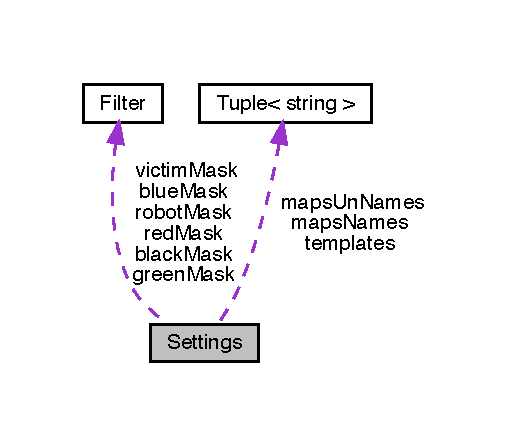
\includegraphics[width=244pt]{class_settings__coll__graph}
\end{center}
\end{figure}
\subsection*{Public Types}
\begin{DoxyCompactItemize}
\item 
enum \mbox{\hyperlink{class_settings_a30d85f2e06a54ae9bc8da2d01037658f}{C\+O\+L\+OR}} \{ \newline
\mbox{\hyperlink{class_settings_a30d85f2e06a54ae9bc8da2d01037658fad72cf235641afa26b82dc5bb8b0db4e1}{B\+L\+A\+CK}}, 
\mbox{\hyperlink{class_settings_a30d85f2e06a54ae9bc8da2d01037658fa164128164b54423f54968a67580a4ce3}{R\+ED}}, 
\mbox{\hyperlink{class_settings_a30d85f2e06a54ae9bc8da2d01037658fa79963b69fcbb589ae6f3f09ac6c5ae90}{G\+R\+E\+EN}}, 
\mbox{\hyperlink{class_settings_a30d85f2e06a54ae9bc8da2d01037658fab4951d8c5bc23e9dab4e9cb53ef3fb26}{V\+I\+C\+T\+I\+MS}}, 
\newline
\mbox{\hyperlink{class_settings_a30d85f2e06a54ae9bc8da2d01037658fa23f16922180d0f5fdc679584f75f83c3}{B\+L\+UE}}, 
\mbox{\hyperlink{class_settings_a30d85f2e06a54ae9bc8da2d01037658fa1cf089d6c6dda465fa704222461f0b28}{R\+O\+B\+OT}}
 \}
\end{DoxyCompactItemize}
\subsection*{Public Member Functions}
\begin{DoxyCompactItemize}
\item 
\mbox{\hyperlink{class_settings_a716069efb4808f2c395dfa218ec1c540}{Settings}} (string \+\_\+base\+Folder=\char`\"{}data/\char`\"{}, string \+\_\+maps\+Folder=\char`\"{}map\char`\"{}, string \+\_\+templates\+Folder=\char`\"{}num\+\_\+template/\char`\"{}, vector$<$ string $>$ \+\_\+maps\+Names=\{\}, vector$<$ string $>$ \+\_\+maps\+Un\+Names=\{\}, string \+\_\+intrinsic\+Calibration\+File=\char`\"{}intrinsic\+\_\+calibration.\+xml\char`\"{}, string \+\_\+calibration\+File=\char`\"{}calib\+\_\+config.\+xml\char`\"{}, Filter \+\_\+black\+Mask=\mbox{\hyperlink{class_filter}{Filter}}(0, 0, 0, 179, 255, 70), \mbox{\hyperlink{class_filter}{Filter}} \+\_\+red\+Mask=\mbox{\hyperlink{class_filter}{Filter}}(15, 100, 140, 160, 255, 255), \mbox{\hyperlink{class_filter}{Filter}} \+\_\+green\+Mask=\mbox{\hyperlink{class_filter}{Filter}}(54, 74, 25, 119, 255, 88), \mbox{\hyperlink{class_filter}{Filter}} \+\_\+victim\+Mask=\mbox{\hyperlink{class_filter}{Filter}}(0, 0, 0, 179, 255, 80), \mbox{\hyperlink{class_filter}{Filter}} \+\_\+blue\+Mask=\mbox{\hyperlink{class_filter}{Filter}}(100, 100, 40, 140, 200, 170), \mbox{\hyperlink{class_filter}{Filter}} \+\_\+robote\+Mask=\mbox{\hyperlink{class_filter}{Filter}}(100, 100, 40, 140, 200, 170), \mbox{\hyperlink{draw_8hh_aa620a13339ac3a1177c86edc549fda9b}{int}} \+\_\+kernel\+Side=9, string \+\_\+convex\+Hull\+File=\char`\"{}convex\+Hull.\+xml\char`\"{}, vector$<$ string $>$ \+\_\+templates=\{\})
\begin{DoxyCompactList}\small\item\em Constructor of class \mbox{\hyperlink{class_settings}{Settings}}. The value are all set by default. The constructor does N\+OT read from or write to file. \end{DoxyCompactList}\item 
\mbox{\hyperlink{class_settings_a4a65be5921dfc9fddc476e5320541d89}{$\sim$\+Settings}} ()
\begin{DoxyCompactList}\small\item\em Destructor. \end{DoxyCompactList}\item 
void \mbox{\hyperlink{class_settings_a14ebf63b888dd7ecf7a34de9eaba1ae8}{save}} (string \+\_\+base\+Folder=\char`\"{}data/\char`\"{}, string \+\_\+maps\+Folder=\char`\"{}map/\char`\"{}, string \+\_\+templates\+Folder=\char`\"{}num\+\_\+template/\char`\"{}, vector$<$ string $>$ \+\_\+maps\+Names=\{\}, vector$<$ string $>$ \+\_\+maps\+Un\+Names=\{\}, string \+\_\+intrinsic\+Calibration\+File=\char`\"{}intrinsic\+\_\+calibration.\+xml\char`\"{}, string \+\_\+calibration\+File=\char`\"{}calib\+\_\+config.\+xml\char`\"{}, Filter \+\_\+black\+Mask=\mbox{\hyperlink{class_filter}{Filter}}(0, 0, 0, 179, 255, 70), \mbox{\hyperlink{class_filter}{Filter}} \+\_\+red\+Mask=\mbox{\hyperlink{class_filter}{Filter}}(15, 100, 140, 160, 255, 255), \mbox{\hyperlink{class_filter}{Filter}} \+\_\+green\+Mask=\mbox{\hyperlink{class_filter}{Filter}}(54, 74, 25, 119, 255, 88), \mbox{\hyperlink{class_filter}{Filter}} \+\_\+victim\+Mask=\mbox{\hyperlink{class_filter}{Filter}}(0, 0, 0, 179, 255, 80), \mbox{\hyperlink{class_filter}{Filter}} \+\_\+blue\+Mask=\mbox{\hyperlink{class_filter}{Filter}}(100, 100, 40, 140, 200, 170), \mbox{\hyperlink{class_filter}{Filter}} \+\_\+robote\+Mask=\mbox{\hyperlink{class_filter}{Filter}}(100, 100, 40, 140, 200, 170), \mbox{\hyperlink{draw_8hh_aa620a13339ac3a1177c86edc549fda9b}{int}} \+\_\+kernel\+Side=9, string \+\_\+convex\+Hull\+File=\char`\"{}convex\+Hull.\+xml\char`\"{}, vector$<$ string $>$ \+\_\+templates=\{\})
\begin{DoxyCompactList}\small\item\em Function to change values. The value are all set by default. This function does N\+OT read from or write to file. \end{DoxyCompactList}\item 
void \mbox{\hyperlink{class_settings_a69b5dc81f8928efdcfc19e409f6015fb}{write\+To\+File}} (string \+\_\+path=\char`\"{}\char`\"{})
\begin{DoxyCompactList}\small\item\em Function to write settings to file. Default is data/settings.\+xml. \end{DoxyCompactList}\item 
void \mbox{\hyperlink{class_settings_a8491d82663ed43dadc540c4a402156fc}{read\+From\+File}} (string \+\_\+path=\char`\"{}\char`\"{})
\begin{DoxyCompactList}\small\item\em Function to read from file. The data found is going to be added to the settings. Default file is data/settings.\+xml. \end{DoxyCompactList}\item 
void \mbox{\hyperlink{class_settings_a8ad60105ab9848720d05ebd19c5063f2}{clean}} ()
\begin{DoxyCompactList}\small\item\em Function to clean all settings\+: number types are set to 0, string are set to \char`\"{}\char`\"{}, Tuples are set to Tuple$<$$>$() and \mbox{\hyperlink{class_filter}{Filter}} are set to all 0s. \end{DoxyCompactList}\item 
void \mbox{\hyperlink{class_settings_acd13c0d603d94c7c2da58cd92bc955c8}{clean\+And\+Read}} (string \+\_\+path=\char`\"{}\char`\"{})
\begin{DoxyCompactList}\small\item\em Function to clean all settings and then read from file. If no path is given the base\+Folder is used. \end{DoxyCompactList}\item 
\mbox{\hyperlink{class_tuple}{Tuple}}$<$ string $>$ \mbox{\hyperlink{class_settings_aa924e455cc6ac356ba6a4c59ab09591c}{maps}} (\mbox{\hyperlink{class_tuple}{Tuple}}$<$ \mbox{\hyperlink{draw_8hh_aa620a13339ac3a1177c86edc549fda9b}{int}} $>$ ids=\mbox{\hyperlink{class_tuple}{Tuple}}$<$ \mbox{\hyperlink{draw_8hh_aa620a13339ac3a1177c86edc549fda9b}{int}} $>$())
\begin{DoxyCompactList}\small\item\em Function to return the paths of maps. If ids are not specified all maps are returned. \end{DoxyCompactList}\item 
\mbox{\hyperlink{class_tuple}{Tuple}}$<$ string $>$ \mbox{\hyperlink{class_settings_adc050f187f4040f5e897b2ff41caedd0}{maps}} (\mbox{\hyperlink{draw_8hh_aa620a13339ac3a1177c86edc549fda9b}{int}} id=-\/1)
\begin{DoxyCompactList}\small\item\em Function to return the path of a map. If id is negative all maps are returned. \end{DoxyCompactList}\item 
string \mbox{\hyperlink{class_settings_aa34e6004beffad1bc5fd81f99353d3e1}{maps}} (string \+\_\+map\+Name)
\begin{DoxyCompactList}\small\item\em A function to return the path of a given map. \end{DoxyCompactList}\item 
\mbox{\hyperlink{class_tuple}{Tuple}}$<$ string $>$ \mbox{\hyperlink{class_settings_ab638c9895f57ed5e8ab64084752c660d}{maps}} (\mbox{\hyperlink{class_tuple}{Tuple}}$<$ string $>$ \+\_\+map\+Names)
\begin{DoxyCompactList}\small\item\em A function to return the paths of a given \mbox{\hyperlink{class_tuple}{Tuple}} of maps. \end{DoxyCompactList}\item 
bool \mbox{\hyperlink{class_settings_aeee4537bd39c18ca3a711a73c9c2277e}{add\+Un\+Map}} (string un\+Map)
\begin{DoxyCompactList}\small\item\em Adds the name of an undistorted map to the list. \end{DoxyCompactList}\item 
\mbox{\hyperlink{class_tuple}{Tuple}}$<$ string $>$ \mbox{\hyperlink{class_settings_a7cbf0234eaca6582ce982f0cf756d282}{un\+Maps}} (\mbox{\hyperlink{class_tuple}{Tuple}}$<$ \mbox{\hyperlink{draw_8hh_aa620a13339ac3a1177c86edc549fda9b}{int}} $>$ ids=\mbox{\hyperlink{class_tuple}{Tuple}}$<$ \mbox{\hyperlink{draw_8hh_aa620a13339ac3a1177c86edc549fda9b}{int}} $>$())
\begin{DoxyCompactList}\small\item\em Function to return the paths of undistorted maps. If ids are not specified all undistorted maps are returned. \end{DoxyCompactList}\item 
\mbox{\hyperlink{class_tuple}{Tuple}}$<$ string $>$ \mbox{\hyperlink{class_settings_a0619c378aff05b5762afe0280b40e07a}{un\+Maps}} (\mbox{\hyperlink{draw_8hh_aa620a13339ac3a1177c86edc549fda9b}{int}} id=-\/1)
\begin{DoxyCompactList}\small\item\em Function to return the path of an undistorted map. If id is negative all undistorted maps are returned. \end{DoxyCompactList}\item 
string \mbox{\hyperlink{class_settings_a6e62c5eb18f6abc4bcbcd11e018fda8b}{un\+Maps}} (string \+\_\+un\+Map\+Name)
\begin{DoxyCompactList}\small\item\em A function to return the path of a given undistorted map. \end{DoxyCompactList}\item 
\mbox{\hyperlink{class_tuple}{Tuple}}$<$ string $>$ \mbox{\hyperlink{class_settings_aa89550d142cb4101faf35af214f4edff}{un\+Maps}} (\mbox{\hyperlink{class_tuple}{Tuple}}$<$ string $>$ \+\_\+un\+Map\+Names)
\begin{DoxyCompactList}\small\item\em A function to return the paths of a given \mbox{\hyperlink{class_tuple}{Tuple}} of undistorted maps. \end{DoxyCompactList}\item 
\mbox{\hyperlink{class_tuple}{Tuple}}$<$ string $>$ \mbox{\hyperlink{class_settings_af68cb84ba3c8d21e004661fee7c0efe7}{get\+Templates}} (\mbox{\hyperlink{draw_8hh_aa620a13339ac3a1177c86edc549fda9b}{int}} id=-\/1)
\begin{DoxyCompactList}\small\item\em Function to return the path of a template. If id is negative all templates are returned. \end{DoxyCompactList}\item 
string \mbox{\hyperlink{class_settings_aa77f9d559fb0f14d551c4ee8a742e6b0}{get\+Templates}} (string \+\_\+template)
\begin{DoxyCompactList}\small\item\em A function to return the path of a given template. \end{DoxyCompactList}\item 
\mbox{\hyperlink{class_tuple}{Tuple}}$<$ string $>$ \mbox{\hyperlink{class_settings_a2fe58de6135c30ec02bccfc20cc15fe3}{get\+Templates}} (\mbox{\hyperlink{class_tuple}{Tuple}}$<$ string $>$ \+\_\+templates)
\begin{DoxyCompactList}\small\item\em A function to return the paths of a given \mbox{\hyperlink{class_tuple}{Tuple}} of templates. \end{DoxyCompactList}\item 
void \mbox{\hyperlink{class_settings_ad0d55c536a84990b048463b924c7d88e}{change\+Mask}} (\mbox{\hyperlink{class_tuple}{Tuple}}$<$ \mbox{\hyperlink{class_settings_a30d85f2e06a54ae9bc8da2d01037658f}{C\+O\+L\+OR}} $>$ color, \mbox{\hyperlink{class_tuple}{Tuple}}$<$ \mbox{\hyperlink{class_filter}{Filter}} $>$ fil)
\begin{DoxyCompactList}\small\item\em Change the values of \mbox{\hyperlink{class_tuple}{Tuple}} of filters. Mind that no write function is called. \end{DoxyCompactList}\item 
void \mbox{\hyperlink{class_settings_ad00eb6c82b7e6af5afbb8d881c50dea8}{change\+Mask}} (\mbox{\hyperlink{class_settings_a30d85f2e06a54ae9bc8da2d01037658f}{C\+O\+L\+OR}} color, \mbox{\hyperlink{class_filter}{Filter}} fil)
\begin{DoxyCompactList}\small\item\em Change the values of a filter. Mind that no write function is called. \end{DoxyCompactList}\item 
stringstream \mbox{\hyperlink{class_settings_a20696223267b07d77408e38e87388274}{to\+\_\+string}} () const
\begin{DoxyCompactList}\small\item\em A function that creates a stringstream to print the values stored in settings. \end{DoxyCompactList}\end{DoxyCompactItemize}
\subsection*{Public Attributes}
\begin{DoxyCompactItemize}
\item 
string \mbox{\hyperlink{class_settings_ae48d5bd7db6c75ba5c697e08e4b32cee}{base\+Folder}}
\begin{DoxyCompactList}\small\item\em A string containing the path for the base dir of data. \end{DoxyCompactList}\item 
string \mbox{\hyperlink{class_settings_aeddfd4457036a14cb0a48d50d9e6ccfe}{maps\+Folder}}
\begin{DoxyCompactList}\small\item\em A string containing the name for maps folder. No certainty is given about the form of this string. \end{DoxyCompactList}\item 
\mbox{\hyperlink{class_tuple}{Tuple}}$<$ string $>$ \mbox{\hyperlink{class_settings_a4a464c938e96639861dc2deb773a2fb8}{maps\+Names}}
\begin{DoxyCompactList}\small\item\em A \mbox{\hyperlink{class_tuple}{Tuple}} containing the names of the maps. These are not paths but just names. \end{DoxyCompactList}\item 
\mbox{\hyperlink{class_tuple}{Tuple}}$<$ string $>$ \mbox{\hyperlink{class_settings_a1866d578ad33e56429a88617a655f9c6}{maps\+Un\+Names}}
\begin{DoxyCompactList}\small\item\em A \mbox{\hyperlink{class_tuple}{Tuple}} containing the names of the undistorted maps. These are not paths but just names. \end{DoxyCompactList}\item 
string \mbox{\hyperlink{class_settings_a634e9900615e8d5b46b08e0fc86d67a5}{intrinsic\+Calibration\+File}}
\begin{DoxyCompactList}\small\item\em A string containing the name to the file containing the values of the matrix for the calibration. \end{DoxyCompactList}\item 
string \mbox{\hyperlink{class_settings_ac6ff9ca8d90b9e43e26c069c88b7c699}{calibration\+File}}
\begin{DoxyCompactList}\small\item\em A string containing the name to the file containing the data for the calibration. \end{DoxyCompactList}\item 
\mbox{\hyperlink{class_filter}{Filter}} \mbox{\hyperlink{class_settings_a78ac37593a52a83973e18deefb2cc96c}{black\+Mask}}
\begin{DoxyCompactList}\small\item\em \mbox{\hyperlink{class_filter}{Filter}} for black. \end{DoxyCompactList}\item 
\mbox{\hyperlink{class_filter}{Filter}} \mbox{\hyperlink{class_settings_a4ded995ae1c425f92ad712d2987dce71}{red\+Mask}}
\begin{DoxyCompactList}\small\item\em \mbox{\hyperlink{class_filter}{Filter}} for red. \end{DoxyCompactList}\item 
\mbox{\hyperlink{class_filter}{Filter}} \mbox{\hyperlink{class_settings_a05138be305e15677c8a84ddf27e4d9e8}{green\+Mask}}
\begin{DoxyCompactList}\small\item\em \mbox{\hyperlink{class_filter}{Filter}} for green. \end{DoxyCompactList}\item 
\mbox{\hyperlink{class_filter}{Filter}} \mbox{\hyperlink{class_settings_ad77dc9d3ebdc000309f1279bc0f9e1ea}{victim\+Mask}}
\begin{DoxyCompactList}\small\item\em \mbox{\hyperlink{class_filter}{Filter}} for the victims. \end{DoxyCompactList}\item 
\mbox{\hyperlink{class_filter}{Filter}} \mbox{\hyperlink{class_settings_a2b425f747b936e82dfe0b609538f06f1}{blue\+Mask}}
\begin{DoxyCompactList}\small\item\em \mbox{\hyperlink{class_filter}{Filter}} for blue. \end{DoxyCompactList}\item 
\mbox{\hyperlink{class_filter}{Filter}} \mbox{\hyperlink{class_settings_aa814fd0ce673e73de3442e5bf5a26fc6}{robot\+Mask}}
\begin{DoxyCompactList}\small\item\em \mbox{\hyperlink{class_filter}{Filter}} for the triangle above the robot. \end{DoxyCompactList}\item 
\mbox{\hyperlink{draw_8hh_aa620a13339ac3a1177c86edc549fda9b}{int}} \mbox{\hyperlink{class_settings_a376418be10e2c1067b2d03c08e7b6a92}{kernel\+Side}}
\item 
string \mbox{\hyperlink{class_settings_aae9ea78e634fee8a76c2eb2b6fd09eeb}{convex\+Hull\+File}}
\begin{DoxyCompactList}\small\item\em A\+String containing the name to file containing the points of the elements in the arena. \end{DoxyCompactList}\item 
string \mbox{\hyperlink{class_settings_a3c272482637bc9c3a534e08e75157830}{templates\+Folder}}
\begin{DoxyCompactList}\small\item\em A String containing the name of the folder containing the number templates. \end{DoxyCompactList}\item 
\mbox{\hyperlink{class_tuple}{Tuple}}$<$ string $>$ \mbox{\hyperlink{class_settings_add9f0e9a114013a3295ba056e19d991f}{templates}}
\begin{DoxyCompactList}\small\item\em A \mbox{\hyperlink{class_tuple}{Tuple}} containing the names of the templates. These are not paths but just names. \end{DoxyCompactList}\end{DoxyCompactItemize}
\subsection*{Friends}
\begin{DoxyCompactItemize}
\item 
ostream \& \mbox{\hyperlink{class_settings_ae9bfb3fa2d38f0ebe2e74b782790da98}{operator$<$$<$}} (ostream \&out, const \mbox{\hyperlink{class_settings}{Settings}} \&data)
\end{DoxyCompactItemize}


\subsection{Detailed Description}
Class that stores settings for the projects such as location of files, name of maps and filters to use. Mind that when created it does not read from file by default but the function must be invoked. 

\subsection{Member Enumeration Documentation}
\mbox{\Hypertarget{class_settings_a30d85f2e06a54ae9bc8da2d01037658f}\label{class_settings_a30d85f2e06a54ae9bc8da2d01037658f}} 
\index{Settings@{Settings}!COLOR@{COLOR}}
\index{COLOR@{COLOR}!Settings@{Settings}}
\subsubsection{\texorpdfstring{COLOR}{COLOR}}
{\footnotesize\ttfamily enum \mbox{\hyperlink{class_settings_a30d85f2e06a54ae9bc8da2d01037658f}{Settings\+::\+C\+O\+L\+OR}}}

\begin{DoxyEnumFields}{Enumerator}
\raisebox{\heightof{T}}[0pt][0pt]{\index{BLACK@{BLACK}!Settings@{Settings}}\index{Settings@{Settings}!BLACK@{BLACK}}}\mbox{\Hypertarget{class_settings_a30d85f2e06a54ae9bc8da2d01037658fad72cf235641afa26b82dc5bb8b0db4e1}\label{class_settings_a30d85f2e06a54ae9bc8da2d01037658fad72cf235641afa26b82dc5bb8b0db4e1}} 
B\+L\+A\+CK&\\
\hline

\raisebox{\heightof{T}}[0pt][0pt]{\index{RED@{RED}!Settings@{Settings}}\index{Settings@{Settings}!RED@{RED}}}\mbox{\Hypertarget{class_settings_a30d85f2e06a54ae9bc8da2d01037658fa164128164b54423f54968a67580a4ce3}\label{class_settings_a30d85f2e06a54ae9bc8da2d01037658fa164128164b54423f54968a67580a4ce3}} 
R\+ED&\\
\hline

\raisebox{\heightof{T}}[0pt][0pt]{\index{GREEN@{GREEN}!Settings@{Settings}}\index{Settings@{Settings}!GREEN@{GREEN}}}\mbox{\Hypertarget{class_settings_a30d85f2e06a54ae9bc8da2d01037658fa79963b69fcbb589ae6f3f09ac6c5ae90}\label{class_settings_a30d85f2e06a54ae9bc8da2d01037658fa79963b69fcbb589ae6f3f09ac6c5ae90}} 
G\+R\+E\+EN&\\
\hline

\raisebox{\heightof{T}}[0pt][0pt]{\index{VICTIMS@{VICTIMS}!Settings@{Settings}}\index{Settings@{Settings}!VICTIMS@{VICTIMS}}}\mbox{\Hypertarget{class_settings_a30d85f2e06a54ae9bc8da2d01037658fab4951d8c5bc23e9dab4e9cb53ef3fb26}\label{class_settings_a30d85f2e06a54ae9bc8da2d01037658fab4951d8c5bc23e9dab4e9cb53ef3fb26}} 
V\+I\+C\+T\+I\+MS&\\
\hline

\raisebox{\heightof{T}}[0pt][0pt]{\index{BLUE@{BLUE}!Settings@{Settings}}\index{Settings@{Settings}!BLUE@{BLUE}}}\mbox{\Hypertarget{class_settings_a30d85f2e06a54ae9bc8da2d01037658fa23f16922180d0f5fdc679584f75f83c3}\label{class_settings_a30d85f2e06a54ae9bc8da2d01037658fa23f16922180d0f5fdc679584f75f83c3}} 
B\+L\+UE&\\
\hline

\raisebox{\heightof{T}}[0pt][0pt]{\index{ROBOT@{ROBOT}!Settings@{Settings}}\index{Settings@{Settings}!ROBOT@{ROBOT}}}\mbox{\Hypertarget{class_settings_a30d85f2e06a54ae9bc8da2d01037658fa1cf089d6c6dda465fa704222461f0b28}\label{class_settings_a30d85f2e06a54ae9bc8da2d01037658fa1cf089d6c6dda465fa704222461f0b28}} 
R\+O\+B\+OT&\\
\hline

\end{DoxyEnumFields}


\subsection{Constructor \& Destructor Documentation}
\mbox{\Hypertarget{class_settings_a716069efb4808f2c395dfa218ec1c540}\label{class_settings_a716069efb4808f2c395dfa218ec1c540}} 
\index{Settings@{Settings}!Settings@{Settings}}
\index{Settings@{Settings}!Settings@{Settings}}
\subsubsection{\texorpdfstring{Settings()}{Settings()}}
{\footnotesize\ttfamily Settings\+::\+Settings (\begin{DoxyParamCaption}\item[{string}]{\+\_\+base\+Folder = {\ttfamily \char`\"{}data/\char`\"{}},  }\item[{string}]{\+\_\+maps\+Folder = {\ttfamily \char`\"{}map\char`\"{}},  }\item[{string}]{\+\_\+templates\+Folder = {\ttfamily \char`\"{}num\+\_\+template/\char`\"{}},  }\item[{vector$<$ string $>$}]{\+\_\+maps\+Names = {\ttfamily \{\}},  }\item[{vector$<$ string $>$}]{\+\_\+maps\+Un\+Names = {\ttfamily \{\}},  }\item[{string}]{\+\_\+intrinsic\+Calibration\+File = {\ttfamily \char`\"{}intrinsic\+\_\+calibration.xml\char`\"{}},  }\item[{string}]{\+\_\+calibration\+File = {\ttfamily \char`\"{}calib\+\_\+config.xml\char`\"{}},  }\item[{\mbox{\hyperlink{class_filter}{Filter}}}]{\+\_\+black\+Mask = {\ttfamily \mbox{\hyperlink{class_filter}{Filter}}(0,~0,~0,~179,~255,~70)},  }\item[{\mbox{\hyperlink{class_filter}{Filter}}}]{\+\_\+red\+Mask = {\ttfamily \mbox{\hyperlink{class_filter}{Filter}}(15,~100,~140,~160,~255,~255)},  }\item[{\mbox{\hyperlink{class_filter}{Filter}}}]{\+\_\+green\+Mask = {\ttfamily \mbox{\hyperlink{class_filter}{Filter}}(54,~74,~25,~119,~255,~88)},  }\item[{\mbox{\hyperlink{class_filter}{Filter}}}]{\+\_\+victim\+Mask = {\ttfamily \mbox{\hyperlink{class_filter}{Filter}}(0,~0,~0,~179,~255,~80)},  }\item[{\mbox{\hyperlink{class_filter}{Filter}}}]{\+\_\+blue\+Mask = {\ttfamily \mbox{\hyperlink{class_filter}{Filter}}(100,~100,~40,~140,~200,~170)},  }\item[{\mbox{\hyperlink{class_filter}{Filter}}}]{\+\_\+robot\+Mask = {\ttfamily \mbox{\hyperlink{class_filter}{Filter}}(100,~100,~40,~140,~200,~170)},  }\item[{\mbox{\hyperlink{draw_8hh_aa620a13339ac3a1177c86edc549fda9b}{int}}}]{\+\_\+kernel\+Side = {\ttfamily 9},  }\item[{string}]{\+\_\+convex\+Hull\+File = {\ttfamily \char`\"{}convexHull.xml\char`\"{}},  }\item[{vector$<$ string $>$}]{\+\_\+templates = {\ttfamily \{\}} }\end{DoxyParamCaption})}



Constructor of class \mbox{\hyperlink{class_settings}{Settings}}. The value are all set by default. The constructor does N\+OT read from or write to file. 


\begin{DoxyParams}[1]{Parameters}
\mbox{\texttt{ in}}  & {\em base\+Folder} & A string containing the path for the base dir of data. \\
\hline
\mbox{\texttt{ in}}  & {\em maps\+Folder} & A string containing the name for maps folder. No certainty is given about the form of this string. \\
\hline
\mbox{\texttt{ in}}  & {\em \+\_\+templates\+Folder} & A String containing the name of the folder containing the number templates. \\
\hline
\mbox{\texttt{ in}}  & {\em \+\_\+maps\+Names} & A \mbox{\hyperlink{class_tuple}{Tuple}} containing the names of the maps. These are not paths but just names. \\
\hline
\mbox{\texttt{ in}}  & {\em \+\_\+maps\+Un\+Names} & A \mbox{\hyperlink{class_tuple}{Tuple}} containing the names of the undistorted maps. These are not paths but just names. \\
\hline
\mbox{\texttt{ in}}  & {\em \+\_\+calibration\+File} & A string containing the name to the file containing the data for the calibration. \\
\hline
\mbox{\texttt{ in}}  & {\em \+\_\+intrinsic\+Calibration\+File} & A string containing the name to the file containing the values of the matrix for the calibration. \\
\hline
\mbox{\texttt{ in}}  & {\em \+\_\+black\+Mask} & \mbox{\hyperlink{class_filter}{Filter}} for black. \\
\hline
\mbox{\texttt{ in}}  & {\em \+\_\+red\+Mask} & \mbox{\hyperlink{class_filter}{Filter}} for red. \\
\hline
\mbox{\texttt{ in}}  & {\em \+\_\+green\+Mask} & \mbox{\hyperlink{class_filter}{Filter}} for green. \\
\hline
\mbox{\texttt{ in}}  & {\em \+\_\+victim\+Mask} & \mbox{\hyperlink{class_filter}{Filter}} for the victims. \\
\hline
\mbox{\texttt{ in}}  & {\em \+\_\+blue\+Mask} & \mbox{\hyperlink{class_filter}{Filter}} for blue. \\
\hline
\mbox{\texttt{ in}}  & {\em \+\_\+robot\+Mask} & \mbox{\hyperlink{class_filter}{Filter}} for the triangle above the robot. \\
\hline
\mbox{\texttt{ in}}  & {\em \+\_\+kernel\+Side} & \\
\hline
\mbox{\texttt{ in}}  & {\em \+\_\+convex\+Hull\+File} & A String containing the name to file containing the points of the elements in the arena. \\
\hline
\mbox{\texttt{ in}}  & {\em \+\_\+templates} & A \mbox{\hyperlink{class_tuple}{Tuple}} containing the names of the templates. These are not paths but just names.\\
\hline
 & {\em maps\+Folder} & A string containing the path for maps\+Folder. No certainty is given about the form of this string \\
\hline
 & {\em \+\_\+templates\+Folder} & A String containing the path of the folder containing the number templates. \\
\hline
 & {\em \+\_\+maps\+Names} & A \mbox{\hyperlink{class_tuple}{Tuple}} containing the names of the maps. These are not paths but just names. \\
\hline
 & {\em \+\_\+maps\+Un\+Names} & A \mbox{\hyperlink{class_tuple}{Tuple}} containing the names of the undistorted maps. These are not paths but just names. \\
\hline
 & {\em \+\_\+calibration\+File} & A string containing the path to the file containing the data for the calibration. \\
\hline
 & {\em \+\_\+intrinsic\+Calibration\+File} & A string containing the path to the file containing the values of the matrix for the calibration. \\
\hline
 & {\em \+\_\+black\+Mask} & \mbox{\hyperlink{class_filter}{Filter}} for black. \\
\hline
 & {\em \+\_\+red\+Mask} & \mbox{\hyperlink{class_filter}{Filter}} for red. \\
\hline
 & {\em \+\_\+green\+Mask} & \mbox{\hyperlink{class_filter}{Filter}} for green. \\
\hline
 & {\em \+\_\+victim\+Mask} & \mbox{\hyperlink{class_filter}{Filter}} for the victims. \\
\hline
 & {\em \+\_\+blue\+Mask} & \mbox{\hyperlink{class_filter}{Filter}} for blue. \\
\hline
 & {\em \+\_\+robot\+Mask} & \mbox{\hyperlink{class_filter}{Filter}} for the triangle above the robot. \\
\hline
 & {\em \+\_\+kernel\+Side} & \\
\hline
 & {\em \+\_\+convex\+Hull\+File} & A String containing the path to file containing the points of the elements in the arena. \\
\hline
 & {\em \+\_\+templates} & A \mbox{\hyperlink{class_tuple}{Tuple}} containing the names of the templates. These are not paths but just names. \\
\hline
\end{DoxyParams}
\mbox{\Hypertarget{class_settings_a4a65be5921dfc9fddc476e5320541d89}\label{class_settings_a4a65be5921dfc9fddc476e5320541d89}} 
\index{Settings@{Settings}!````~Settings@{$\sim$Settings}}
\index{````~Settings@{$\sim$Settings}!Settings@{Settings}}
\subsubsection{\texorpdfstring{$\sim$Settings()}{~Settings()}}
{\footnotesize\ttfamily Settings\+::$\sim$\+Settings (\begin{DoxyParamCaption}{ }\end{DoxyParamCaption})}



Destructor. 



\subsection{Member Function Documentation}
\mbox{\Hypertarget{class_settings_aeee4537bd39c18ca3a711a73c9c2277e}\label{class_settings_aeee4537bd39c18ca3a711a73c9c2277e}} 
\index{Settings@{Settings}!addUnMap@{addUnMap}}
\index{addUnMap@{addUnMap}!Settings@{Settings}}
\subsubsection{\texorpdfstring{addUnMap()}{addUnMap()}}
{\footnotesize\ttfamily bool Settings\+::add\+Un\+Map (\begin{DoxyParamCaption}\item[{string}]{\+\_\+un\+Map }\end{DoxyParamCaption})}



Adds the name of an undistorted map to the list. 

Adds the name of an undistorted map.


\begin{DoxyParams}[1]{Parameters}
\mbox{\texttt{ in}}  & {\em un\+Map} & The undistorted map\\
\hline
\end{DoxyParams}
\begin{DoxyReturn}{Returns}
{\ttfamily true} of the name of the map could be added, {\ttfamily false} otherwise.
\end{DoxyReturn}

\begin{DoxyParams}[1]{Parameters}
\mbox{\texttt{ in}}  & {\em \+\_\+un\+Map} & The name of the undistorted map \\
\hline
\end{DoxyParams}
\begin{DoxyReturn}{Returns}
{\ttfamily true} if it succeded, {\ttfamily false} otherwise. 
\end{DoxyReturn}
\mbox{\Hypertarget{class_settings_ad0d55c536a84990b048463b924c7d88e}\label{class_settings_ad0d55c536a84990b048463b924c7d88e}} 
\index{Settings@{Settings}!changeMask@{changeMask}}
\index{changeMask@{changeMask}!Settings@{Settings}}
\subsubsection{\texorpdfstring{changeMask()}{changeMask()}\hspace{0.1cm}{\footnotesize\ttfamily [1/2]}}
{\footnotesize\ttfamily void Settings\+::change\+Mask (\begin{DoxyParamCaption}\item[{\mbox{\hyperlink{class_tuple}{Tuple}}$<$ \mbox{\hyperlink{class_settings_a30d85f2e06a54ae9bc8da2d01037658f}{C\+O\+L\+OR}} $>$}]{color,  }\item[{\mbox{\hyperlink{class_tuple}{Tuple}}$<$ \mbox{\hyperlink{class_filter}{Filter}} $>$}]{fil }\end{DoxyParamCaption})}



Change the values of \mbox{\hyperlink{class_tuple}{Tuple}} of filters. Mind that no write function is called. 


\begin{DoxyParams}{Parameters}
{\em color} & A \mbox{\hyperlink{class_tuple}{Tuple}} containing the colors of the filters to change. \\
\hline
{\em fil} & The new filters to be stored. \\
\hline
\end{DoxyParams}
\mbox{\Hypertarget{class_settings_ad00eb6c82b7e6af5afbb8d881c50dea8}\label{class_settings_ad00eb6c82b7e6af5afbb8d881c50dea8}} 
\index{Settings@{Settings}!changeMask@{changeMask}}
\index{changeMask@{changeMask}!Settings@{Settings}}
\subsubsection{\texorpdfstring{changeMask()}{changeMask()}\hspace{0.1cm}{\footnotesize\ttfamily [2/2]}}
{\footnotesize\ttfamily void Settings\+::change\+Mask (\begin{DoxyParamCaption}\item[{\mbox{\hyperlink{class_settings_a30d85f2e06a54ae9bc8da2d01037658f}{C\+O\+L\+OR}}}]{color,  }\item[{\mbox{\hyperlink{class_filter}{Filter}}}]{fil }\end{DoxyParamCaption})}



Change the values of a filter. Mind that no write function is called. 


\begin{DoxyParams}{Parameters}
{\em color} & The filter to change. \\
\hline
{\em fil} & The new filter to be stored. \\
\hline
\end{DoxyParams}
\mbox{\Hypertarget{class_settings_a8ad60105ab9848720d05ebd19c5063f2}\label{class_settings_a8ad60105ab9848720d05ebd19c5063f2}} 
\index{Settings@{Settings}!clean@{clean}}
\index{clean@{clean}!Settings@{Settings}}
\subsubsection{\texorpdfstring{clean()}{clean()}}
{\footnotesize\ttfamily void Settings\+::clean (\begin{DoxyParamCaption}{ }\end{DoxyParamCaption})}



Function to clean all settings\+: number types are set to 0, string are set to \char`\"{}\char`\"{}, Tuples are set to Tuple$<$$>$() and \mbox{\hyperlink{class_filter}{Filter}} are set to all 0s. 

\mbox{\Hypertarget{class_settings_acd13c0d603d94c7c2da58cd92bc955c8}\label{class_settings_acd13c0d603d94c7c2da58cd92bc955c8}} 
\index{Settings@{Settings}!cleanAndRead@{cleanAndRead}}
\index{cleanAndRead@{cleanAndRead}!Settings@{Settings}}
\subsubsection{\texorpdfstring{cleanAndRead()}{cleanAndRead()}}
{\footnotesize\ttfamily void Settings\+::clean\+And\+Read (\begin{DoxyParamCaption}\item[{string}]{\+\_\+path = {\ttfamily \char`\"{}\char`\"{}} }\end{DoxyParamCaption})}



Function to clean all settings and then read from file. If no path is given the base\+Folder is used. 

Function to clean all settings and then read from file. Default is data/settings.\+xml.


\begin{DoxyParams}[1]{Parameters}
\mbox{\texttt{ in}}  & {\em \+\_\+path} & Path to the file. Mind that it doesn\textquotesingle{}t require the name of the file.\\
\hline
\end{DoxyParams}
\mbox{\Hypertarget{class_settings_af68cb84ba3c8d21e004661fee7c0efe7}\label{class_settings_af68cb84ba3c8d21e004661fee7c0efe7}} 
\index{Settings@{Settings}!getTemplates@{getTemplates}}
\index{getTemplates@{getTemplates}!Settings@{Settings}}
\subsubsection{\texorpdfstring{getTemplates()}{getTemplates()}\hspace{0.1cm}{\footnotesize\ttfamily [1/3]}}
{\footnotesize\ttfamily \mbox{\hyperlink{class_tuple}{Tuple}}$<$ string $>$ Settings\+::get\+Templates (\begin{DoxyParamCaption}\item[{\mbox{\hyperlink{draw_8hh_aa620a13339ac3a1177c86edc549fda9b}{int}}}]{id = {\ttfamily -\/1} }\end{DoxyParamCaption})}



Function to return the path of a template. If id is negative all templates are returned. 

Function to return the path of a template. If id is not specified all templates are returned.


\begin{DoxyParams}{Parameters}
{\em id} & The positions in this.\+templates of the template to be retrieved \\
\hline
\end{DoxyParams}
\begin{DoxyReturn}{Returns}
A \mbox{\hyperlink{class_tuple}{Tuple}} containing the paths of the templates. 
\end{DoxyReturn}
\mbox{\Hypertarget{class_settings_aa77f9d559fb0f14d551c4ee8a742e6b0}\label{class_settings_aa77f9d559fb0f14d551c4ee8a742e6b0}} 
\index{Settings@{Settings}!getTemplates@{getTemplates}}
\index{getTemplates@{getTemplates}!Settings@{Settings}}
\subsubsection{\texorpdfstring{getTemplates()}{getTemplates()}\hspace{0.1cm}{\footnotesize\ttfamily [2/3]}}
{\footnotesize\ttfamily string Settings\+::get\+Templates (\begin{DoxyParamCaption}\item[{string}]{\+\_\+template }\end{DoxyParamCaption})}



A function to return the path of a given template. 


\begin{DoxyParams}{Parameters}
{\em \+\_\+template\+Name} & The name of the template to check in the \mbox{\hyperlink{class_tuple}{Tuple}}. \\
\hline
\end{DoxyParams}
\begin{DoxyReturn}{Returns}
The path to the template if it is found, an empty string otherwise. 
\end{DoxyReturn}
\mbox{\Hypertarget{class_settings_a2fe58de6135c30ec02bccfc20cc15fe3}\label{class_settings_a2fe58de6135c30ec02bccfc20cc15fe3}} 
\index{Settings@{Settings}!getTemplates@{getTemplates}}
\index{getTemplates@{getTemplates}!Settings@{Settings}}
\subsubsection{\texorpdfstring{getTemplates()}{getTemplates()}\hspace{0.1cm}{\footnotesize\ttfamily [3/3]}}
{\footnotesize\ttfamily \mbox{\hyperlink{class_tuple}{Tuple}}$<$ string $>$ Settings\+::get\+Templates (\begin{DoxyParamCaption}\item[{\mbox{\hyperlink{class_tuple}{Tuple}}$<$ string $>$}]{\+\_\+templates }\end{DoxyParamCaption})}



A function to return the paths of a given \mbox{\hyperlink{class_tuple}{Tuple}} of templates. 


\begin{DoxyParams}{Parameters}
{\em \+\_\+template} & A \mbox{\hyperlink{class_tuple}{Tuple}} containing the names of the templates to check in the \mbox{\hyperlink{class_tuple}{Tuple}}. \\
\hline
\end{DoxyParams}
\begin{DoxyReturn}{Returns}
The paths to the templates if they are found, an empty \mbox{\hyperlink{class_tuple}{Tuple}} otherwise. 
\end{DoxyReturn}
\mbox{\Hypertarget{class_settings_aa924e455cc6ac356ba6a4c59ab09591c}\label{class_settings_aa924e455cc6ac356ba6a4c59ab09591c}} 
\index{Settings@{Settings}!maps@{maps}}
\index{maps@{maps}!Settings@{Settings}}
\subsubsection{\texorpdfstring{maps()}{maps()}\hspace{0.1cm}{\footnotesize\ttfamily [1/4]}}
{\footnotesize\ttfamily \mbox{\hyperlink{class_tuple}{Tuple}}$<$ string $>$ Settings\+::maps (\begin{DoxyParamCaption}\item[{\mbox{\hyperlink{class_tuple}{Tuple}}$<$ \mbox{\hyperlink{draw_8hh_aa620a13339ac3a1177c86edc549fda9b}{int}} $>$}]{ids = {\ttfamily \mbox{\hyperlink{class_tuple}{Tuple}}$<$\mbox{\hyperlink{draw_8hh_aa620a13339ac3a1177c86edc549fda9b}{int}}$>$()} }\end{DoxyParamCaption})}



Function to return the paths of maps. If ids are not specified all maps are returned. 


\begin{DoxyParams}{Parameters}
{\em ids} & A \mbox{\hyperlink{class_tuple}{Tuple}} containing the ids (that is the positions in this.\+maps\+Names) of the maps to be retrieved. \\
\hline
\end{DoxyParams}
\begin{DoxyReturn}{Returns}
A \mbox{\hyperlink{class_tuple}{Tuple}} containing the paths of the maps. 
\end{DoxyReturn}
\mbox{\Hypertarget{class_settings_adc050f187f4040f5e897b2ff41caedd0}\label{class_settings_adc050f187f4040f5e897b2ff41caedd0}} 
\index{Settings@{Settings}!maps@{maps}}
\index{maps@{maps}!Settings@{Settings}}
\subsubsection{\texorpdfstring{maps()}{maps()}\hspace{0.1cm}{\footnotesize\ttfamily [2/4]}}
{\footnotesize\ttfamily \mbox{\hyperlink{class_tuple}{Tuple}}$<$ string $>$ Settings\+::maps (\begin{DoxyParamCaption}\item[{\mbox{\hyperlink{draw_8hh_aa620a13339ac3a1177c86edc549fda9b}{int}}}]{id = {\ttfamily -\/1} }\end{DoxyParamCaption})}



Function to return the path of a map. If id is negative all maps are returned. 

Function to return the path of a map. If id is not specified all maps are returned.


\begin{DoxyParams}{Parameters}
{\em id} & The positions in this.\+maps\+Names of the map to be retrieved \\
\hline
\end{DoxyParams}
\begin{DoxyReturn}{Returns}
A \mbox{\hyperlink{class_tuple}{Tuple}} containing the paths of the maps.
\end{DoxyReturn}

\begin{DoxyParams}{Parameters}
{\em id} & A the positions in this.\+maps\+Names of the map to be retrieved \\
\hline
\end{DoxyParams}
\begin{DoxyReturn}{Returns}
A \mbox{\hyperlink{class_tuple}{Tuple}} containing the paths of the maps. 
\end{DoxyReturn}
\mbox{\Hypertarget{class_settings_aa34e6004beffad1bc5fd81f99353d3e1}\label{class_settings_aa34e6004beffad1bc5fd81f99353d3e1}} 
\index{Settings@{Settings}!maps@{maps}}
\index{maps@{maps}!Settings@{Settings}}
\subsubsection{\texorpdfstring{maps()}{maps()}\hspace{0.1cm}{\footnotesize\ttfamily [3/4]}}
{\footnotesize\ttfamily string Settings\+::maps (\begin{DoxyParamCaption}\item[{string}]{\+\_\+map\+Name }\end{DoxyParamCaption})}



A function to return the path of a given map. 


\begin{DoxyParams}{Parameters}
{\em \+\_\+map\+Name} & The name of the map to check in the \mbox{\hyperlink{class_tuple}{Tuple}}. \\
\hline
\end{DoxyParams}
\begin{DoxyReturn}{Returns}
The path to the map if the map is found, an empty string otherwise. 
\end{DoxyReturn}
\mbox{\Hypertarget{class_settings_ab638c9895f57ed5e8ab64084752c660d}\label{class_settings_ab638c9895f57ed5e8ab64084752c660d}} 
\index{Settings@{Settings}!maps@{maps}}
\index{maps@{maps}!Settings@{Settings}}
\subsubsection{\texorpdfstring{maps()}{maps()}\hspace{0.1cm}{\footnotesize\ttfamily [4/4]}}
{\footnotesize\ttfamily \mbox{\hyperlink{class_tuple}{Tuple}}$<$ string $>$ Settings\+::maps (\begin{DoxyParamCaption}\item[{\mbox{\hyperlink{class_tuple}{Tuple}}$<$ string $>$}]{\+\_\+map\+Names }\end{DoxyParamCaption})}



A function to return the paths of a given \mbox{\hyperlink{class_tuple}{Tuple}} of maps. 


\begin{DoxyParams}{Parameters}
{\em \+\_\+map\+Names} & A \mbox{\hyperlink{class_tuple}{Tuple}} containing the names of the maps to check in the \mbox{\hyperlink{class_tuple}{Tuple}}. \\
\hline
\end{DoxyParams}
\begin{DoxyReturn}{Returns}
The paths to the maps if they are found, an empty \mbox{\hyperlink{class_tuple}{Tuple}} otherwise. 
\end{DoxyReturn}
\mbox{\Hypertarget{class_settings_a8491d82663ed43dadc540c4a402156fc}\label{class_settings_a8491d82663ed43dadc540c4a402156fc}} 
\index{Settings@{Settings}!readFromFile@{readFromFile}}
\index{readFromFile@{readFromFile}!Settings@{Settings}}
\subsubsection{\texorpdfstring{readFromFile()}{readFromFile()}}
{\footnotesize\ttfamily void Settings\+::read\+From\+File (\begin{DoxyParamCaption}\item[{string}]{\+\_\+path = {\ttfamily \char`\"{}\char`\"{}} }\end{DoxyParamCaption})}



Function to read from file. The data found is going to be added to the settings. Default file is data/settings.\+xml. 


\begin{DoxyParams}[1]{Parameters}
\mbox{\texttt{ in}}  & {\em \+\_\+path} & Path to the file. Mind that it doesn\textquotesingle{}t require the name of the file.\\
\hline
 & {\em \+\_\+path} & The path of file to read from. \\
\hline
\end{DoxyParams}
\mbox{\Hypertarget{class_settings_a14ebf63b888dd7ecf7a34de9eaba1ae8}\label{class_settings_a14ebf63b888dd7ecf7a34de9eaba1ae8}} 
\index{Settings@{Settings}!save@{save}}
\index{save@{save}!Settings@{Settings}}
\subsubsection{\texorpdfstring{save()}{save()}}
{\footnotesize\ttfamily void Settings\+::save (\begin{DoxyParamCaption}\item[{string}]{\+\_\+base\+Folder = {\ttfamily \char`\"{}data/\char`\"{}},  }\item[{string}]{\+\_\+maps\+Folder = {\ttfamily \char`\"{}map/\char`\"{}},  }\item[{string}]{\+\_\+templates\+Folder = {\ttfamily \char`\"{}num\+\_\+template/\char`\"{}},  }\item[{vector$<$ string $>$}]{\+\_\+maps\+Names = {\ttfamily \{\}},  }\item[{vector$<$ string $>$}]{\+\_\+maps\+Un\+Names = {\ttfamily \{\}},  }\item[{string}]{\+\_\+intrinsic\+Calibration\+File = {\ttfamily \char`\"{}intrinsic\+\_\+calibration.xml\char`\"{}},  }\item[{string}]{\+\_\+calibration\+File = {\ttfamily \char`\"{}calib\+\_\+config.xml\char`\"{}},  }\item[{\mbox{\hyperlink{class_filter}{Filter}}}]{\+\_\+black\+Mask = {\ttfamily \mbox{\hyperlink{class_filter}{Filter}}(0,~0,~0,~179,~255,~70)},  }\item[{\mbox{\hyperlink{class_filter}{Filter}}}]{\+\_\+red\+Mask = {\ttfamily \mbox{\hyperlink{class_filter}{Filter}}(15,~100,~140,~160,~255,~255)},  }\item[{\mbox{\hyperlink{class_filter}{Filter}}}]{\+\_\+green\+Mask = {\ttfamily \mbox{\hyperlink{class_filter}{Filter}}(54,~74,~25,~119,~255,~88)},  }\item[{\mbox{\hyperlink{class_filter}{Filter}}}]{\+\_\+victim\+Mask = {\ttfamily \mbox{\hyperlink{class_filter}{Filter}}(0,~0,~0,~179,~255,~80)},  }\item[{\mbox{\hyperlink{class_filter}{Filter}}}]{\+\_\+blue\+Mask = {\ttfamily \mbox{\hyperlink{class_filter}{Filter}}(100,~100,~40,~140,~200,~170)},  }\item[{\mbox{\hyperlink{class_filter}{Filter}}}]{\+\_\+robot\+Mask = {\ttfamily \mbox{\hyperlink{class_filter}{Filter}}(100,~100,~40,~140,~200,~170)},  }\item[{\mbox{\hyperlink{draw_8hh_aa620a13339ac3a1177c86edc549fda9b}{int}}}]{\+\_\+kernel\+Side = {\ttfamily 9},  }\item[{string}]{\+\_\+convex\+Hull\+File = {\ttfamily \char`\"{}convexHull.xml\char`\"{}},  }\item[{vector$<$ string $>$}]{\+\_\+templates = {\ttfamily \{\}} }\end{DoxyParamCaption})}



Function to change values. The value are all set by default. This function does N\+OT read from or write to file. 


\begin{DoxyParams}[1]{Parameters}
\mbox{\texttt{ in}}  & {\em base\+Folder} & A string containing the path for the base dir of data. \\
\hline
\mbox{\texttt{ in}}  & {\em maps\+Folder} & A string containing the name for maps\+Folder. No certainty is given about the form of this string \\
\hline
\mbox{\texttt{ in}}  & {\em \+\_\+templates\+Folder} & A String containing the name of the folder containing the number templates. \\
\hline
\mbox{\texttt{ in}}  & {\em \+\_\+maps\+Names} & A \mbox{\hyperlink{class_tuple}{Tuple}} containing the names of the maps. These are not paths but just names. \\
\hline
\mbox{\texttt{ in}}  & {\em \+\_\+maps\+Un\+Names} & A \mbox{\hyperlink{class_tuple}{Tuple}} containing the names of the undistorted maps. These are not paths but just names. \\
\hline
\mbox{\texttt{ in}}  & {\em \+\_\+calibration\+File} & A string containing the name to the file containing the data for the calibration. \\
\hline
\mbox{\texttt{ in}}  & {\em \+\_\+intrinsic\+Calibration\+File} & A string containing the name to the file containing the values of the matrix for the calibration. \\
\hline
\mbox{\texttt{ in}}  & {\em \+\_\+black\+Mask} & \mbox{\hyperlink{class_filter}{Filter}} for black. \\
\hline
\mbox{\texttt{ in}}  & {\em \+\_\+red\+Mask} & \mbox{\hyperlink{class_filter}{Filter}} for red. \\
\hline
\mbox{\texttt{ in}}  & {\em \+\_\+green\+Mask} & \mbox{\hyperlink{class_filter}{Filter}} for green. \\
\hline
\mbox{\texttt{ in}}  & {\em \+\_\+victim\+Mask} & \mbox{\hyperlink{class_filter}{Filter}} for the victims. \\
\hline
\mbox{\texttt{ in}}  & {\em \+\_\+blue\+Mask} & \mbox{\hyperlink{class_filter}{Filter}} for blue. \\
\hline
\mbox{\texttt{ in}}  & {\em \+\_\+robot\+Mask} & \mbox{\hyperlink{class_filter}{Filter}} for the triangle above the robot. \\
\hline
\mbox{\texttt{ in}}  & {\em \+\_\+kernel\+Side} & \\
\hline
\mbox{\texttt{ in}}  & {\em \+\_\+convex\+Hull\+File} & A String containing the name to file containing the points of the elements in the arena. \\
\hline
\mbox{\texttt{ in}}  & {\em \+\_\+templates} & A \mbox{\hyperlink{class_tuple}{Tuple}} containing the names of the templates. These are not paths but just names.\\
\hline
 & {\em maps\+Folder} & A string containing the path for maps\+Folder. No certainty is given about the form of this string \\
\hline
 & {\em \+\_\+templates\+Folder} & A String containing the path of the folder containing the number templates. \\
\hline
 & {\em \+\_\+maps\+Names} & A \mbox{\hyperlink{class_tuple}{Tuple}} containing the names of the maps. These are not paths but just names. \\
\hline
 & {\em \+\_\+maps\+Un\+Names} & A \mbox{\hyperlink{class_tuple}{Tuple}} containing the names of the undistorted maps. These are not paths but just names. \\
\hline
 & {\em \+\_\+intrinsic\+Calibration\+File} & A string containing the path to the file containing the values of the matrix for the calibration. \\
\hline
 & {\em \+\_\+calibration\+File} & A string containing the path to the file containing the data for the calibration. \\
\hline
 & {\em \+\_\+black\+Mask} & \mbox{\hyperlink{class_filter}{Filter}} for black. \\
\hline
 & {\em \+\_\+red\+Mask} & \mbox{\hyperlink{class_filter}{Filter}} for red. \\
\hline
 & {\em \+\_\+green\+Mask} & \mbox{\hyperlink{class_filter}{Filter}} for green. \\
\hline
 & {\em \+\_\+victim\+Mask} & \mbox{\hyperlink{class_filter}{Filter}} for the victims. \\
\hline
 & {\em \+\_\+blue\+Mask} & \mbox{\hyperlink{class_filter}{Filter}} for blue. \\
\hline
 & {\em \+\_\+robot\+Mask} & \mbox{\hyperlink{class_filter}{Filter}} for the triangle above the robot. \\
\hline
 & {\em \+\_\+kernel\+Side} & \\
\hline
 & {\em \+\_\+convex\+Hull\+File} & A String containing the path to file containing the points of the elements in the arena. \\
\hline
 & {\em \+\_\+templates} & A \mbox{\hyperlink{class_tuple}{Tuple}} containing the names of the templates. These are not paths but just names. \\
\hline
\end{DoxyParams}
\mbox{\Hypertarget{class_settings_a20696223267b07d77408e38e87388274}\label{class_settings_a20696223267b07d77408e38e87388274}} 
\index{Settings@{Settings}!to\_string@{to\_string}}
\index{to\_string@{to\_string}!Settings@{Settings}}
\subsubsection{\texorpdfstring{to\_string()}{to\_string()}}
{\footnotesize\ttfamily stringstream Settings\+::to\+\_\+string (\begin{DoxyParamCaption}{ }\end{DoxyParamCaption}) const\hspace{0.3cm}{\ttfamily [inline]}}



A function that creates a stringstream to print the values stored in settings. 

\begin{DoxyReturn}{Returns}
A strinstream containing the settings values. 
\end{DoxyReturn}
\mbox{\Hypertarget{class_settings_a7cbf0234eaca6582ce982f0cf756d282}\label{class_settings_a7cbf0234eaca6582ce982f0cf756d282}} 
\index{Settings@{Settings}!unMaps@{unMaps}}
\index{unMaps@{unMaps}!Settings@{Settings}}
\subsubsection{\texorpdfstring{unMaps()}{unMaps()}\hspace{0.1cm}{\footnotesize\ttfamily [1/4]}}
{\footnotesize\ttfamily \mbox{\hyperlink{class_tuple}{Tuple}}$<$ string $>$ Settings\+::un\+Maps (\begin{DoxyParamCaption}\item[{\mbox{\hyperlink{class_tuple}{Tuple}}$<$ \mbox{\hyperlink{draw_8hh_aa620a13339ac3a1177c86edc549fda9b}{int}} $>$}]{ids = {\ttfamily \mbox{\hyperlink{class_tuple}{Tuple}}$<$\mbox{\hyperlink{draw_8hh_aa620a13339ac3a1177c86edc549fda9b}{int}}$>$()} }\end{DoxyParamCaption})}



Function to return the paths of undistorted maps. If ids are not specified all undistorted maps are returned. 


\begin{DoxyParams}{Parameters}
{\em ids} & A \mbox{\hyperlink{class_tuple}{Tuple}} containing the ids (that is the positions in this.\+maps\+Un\+Names) of the undistorted maps to be retrieved. \\
\hline
\end{DoxyParams}
\begin{DoxyReturn}{Returns}
A \mbox{\hyperlink{class_tuple}{Tuple}} containing the paths of the undistorted maps. 
\end{DoxyReturn}
\mbox{\Hypertarget{class_settings_a0619c378aff05b5762afe0280b40e07a}\label{class_settings_a0619c378aff05b5762afe0280b40e07a}} 
\index{Settings@{Settings}!unMaps@{unMaps}}
\index{unMaps@{unMaps}!Settings@{Settings}}
\subsubsection{\texorpdfstring{unMaps()}{unMaps()}\hspace{0.1cm}{\footnotesize\ttfamily [2/4]}}
{\footnotesize\ttfamily \mbox{\hyperlink{class_tuple}{Tuple}}$<$ string $>$ Settings\+::un\+Maps (\begin{DoxyParamCaption}\item[{\mbox{\hyperlink{draw_8hh_aa620a13339ac3a1177c86edc549fda9b}{int}}}]{id = {\ttfamily -\/1} }\end{DoxyParamCaption})}



Function to return the path of an undistorted map. If id is negative all undistorted maps are returned. 

Function to return the path of an undistorted map. If id is not specified all undistorted maps are returned.


\begin{DoxyParams}{Parameters}
{\em id} & The positions in this.\+maps\+Un\+Names of the undistorted map to be retrieved \\
\hline
\end{DoxyParams}
\begin{DoxyReturn}{Returns}
A \mbox{\hyperlink{class_tuple}{Tuple}} containing the paths of the undistorted maps.
\end{DoxyReturn}

\begin{DoxyParams}{Parameters}
{\em id} & A the positions in this.\+maps\+Un\+Names of the undistorted map to be retrieved \\
\hline
\end{DoxyParams}
\begin{DoxyReturn}{Returns}
A \mbox{\hyperlink{class_tuple}{Tuple}} containing the paths of the undistorted maps. 
\end{DoxyReturn}
\mbox{\Hypertarget{class_settings_a6e62c5eb18f6abc4bcbcd11e018fda8b}\label{class_settings_a6e62c5eb18f6abc4bcbcd11e018fda8b}} 
\index{Settings@{Settings}!unMaps@{unMaps}}
\index{unMaps@{unMaps}!Settings@{Settings}}
\subsubsection{\texorpdfstring{unMaps()}{unMaps()}\hspace{0.1cm}{\footnotesize\ttfamily [3/4]}}
{\footnotesize\ttfamily string Settings\+::un\+Maps (\begin{DoxyParamCaption}\item[{string}]{\+\_\+un\+Map\+Name }\end{DoxyParamCaption})}



A function to return the path of a given undistorted map. 


\begin{DoxyParams}{Parameters}
{\em \+\_\+un\+Map\+Name} & The name of the undistorted map to check in the \mbox{\hyperlink{class_tuple}{Tuple}}. \\
\hline
\end{DoxyParams}
\begin{DoxyReturn}{Returns}
The path to the undistorted map if it is found, an empty string otherwise. 
\end{DoxyReturn}
\mbox{\Hypertarget{class_settings_aa89550d142cb4101faf35af214f4edff}\label{class_settings_aa89550d142cb4101faf35af214f4edff}} 
\index{Settings@{Settings}!unMaps@{unMaps}}
\index{unMaps@{unMaps}!Settings@{Settings}}
\subsubsection{\texorpdfstring{unMaps()}{unMaps()}\hspace{0.1cm}{\footnotesize\ttfamily [4/4]}}
{\footnotesize\ttfamily \mbox{\hyperlink{class_tuple}{Tuple}}$<$ string $>$ Settings\+::un\+Maps (\begin{DoxyParamCaption}\item[{\mbox{\hyperlink{class_tuple}{Tuple}}$<$ string $>$}]{\+\_\+un\+Map\+Names }\end{DoxyParamCaption})}



A function to return the paths of a given \mbox{\hyperlink{class_tuple}{Tuple}} of undistorted maps. 


\begin{DoxyParams}{Parameters}
{\em \+\_\+un\+Map\+Names} & A \mbox{\hyperlink{class_tuple}{Tuple}} containing the names of the undistorted maps to check in the \mbox{\hyperlink{class_tuple}{Tuple}}. \\
\hline
\end{DoxyParams}
\begin{DoxyReturn}{Returns}
The paths to the undistorted maps if they are found, an empty \mbox{\hyperlink{class_tuple}{Tuple}} otherwise. 
\end{DoxyReturn}
\mbox{\Hypertarget{class_settings_a69b5dc81f8928efdcfc19e409f6015fb}\label{class_settings_a69b5dc81f8928efdcfc19e409f6015fb}} 
\index{Settings@{Settings}!writeToFile@{writeToFile}}
\index{writeToFile@{writeToFile}!Settings@{Settings}}
\subsubsection{\texorpdfstring{writeToFile()}{writeToFile()}}
{\footnotesize\ttfamily void Settings\+::write\+To\+File (\begin{DoxyParamCaption}\item[{string}]{\+\_\+path = {\ttfamily \char`\"{}\char`\"{}} }\end{DoxyParamCaption})}



Function to write settings to file. Default is data/settings.\+xml. 


\begin{DoxyParams}[1]{Parameters}
\mbox{\texttt{ in}}  & {\em \+\_\+path} & Path to the file. Mind that it doesn\textquotesingle{}t require the name of the file.\\
\hline
 & {\em \+\_\+path} & The path of the file to write to. \\
\hline
\end{DoxyParams}


\subsection{Friends And Related Function Documentation}
\mbox{\Hypertarget{class_settings_ae9bfb3fa2d38f0ebe2e74b782790da98}\label{class_settings_ae9bfb3fa2d38f0ebe2e74b782790da98}} 
\index{Settings@{Settings}!operator$<$$<$@{operator$<$$<$}}
\index{operator$<$$<$@{operator$<$$<$}!Settings@{Settings}}
\subsubsection{\texorpdfstring{operator$<$$<$}{operator<<}}
{\footnotesize\ttfamily ostream\& operator$<$$<$ (\begin{DoxyParamCaption}\item[{ostream \&}]{out,  }\item[{const \mbox{\hyperlink{class_settings}{Settings}} \&}]{data }\end{DoxyParamCaption})\hspace{0.3cm}{\ttfamily [friend]}}

This function overload the $<$$<$ operator so to print with {\ttfamily std\+::cout}. 
\begin{DoxyParams}[1]{Parameters}
\mbox{\texttt{ in}}  & {\em out} & The out stream. \\
\hline
\mbox{\texttt{ in}}  & {\em dat\+The} & settings to print. \\
\hline
\end{DoxyParams}
\begin{DoxyReturn}{Returns}
An output stream to be printed. 
\end{DoxyReturn}


\subsection{Member Data Documentation}
\mbox{\Hypertarget{class_settings_ae48d5bd7db6c75ba5c697e08e4b32cee}\label{class_settings_ae48d5bd7db6c75ba5c697e08e4b32cee}} 
\index{Settings@{Settings}!baseFolder@{baseFolder}}
\index{baseFolder@{baseFolder}!Settings@{Settings}}
\subsubsection{\texorpdfstring{baseFolder}{baseFolder}}
{\footnotesize\ttfamily string Settings\+::base\+Folder}



A string containing the path for the base dir of data. 

\mbox{\Hypertarget{class_settings_a78ac37593a52a83973e18deefb2cc96c}\label{class_settings_a78ac37593a52a83973e18deefb2cc96c}} 
\index{Settings@{Settings}!blackMask@{blackMask}}
\index{blackMask@{blackMask}!Settings@{Settings}}
\subsubsection{\texorpdfstring{blackMask}{blackMask}}
{\footnotesize\ttfamily \mbox{\hyperlink{class_filter}{Filter}} Settings\+::black\+Mask}



\mbox{\hyperlink{class_filter}{Filter}} for black. 

\mbox{\Hypertarget{class_settings_a2b425f747b936e82dfe0b609538f06f1}\label{class_settings_a2b425f747b936e82dfe0b609538f06f1}} 
\index{Settings@{Settings}!blueMask@{blueMask}}
\index{blueMask@{blueMask}!Settings@{Settings}}
\subsubsection{\texorpdfstring{blueMask}{blueMask}}
{\footnotesize\ttfamily \mbox{\hyperlink{class_filter}{Filter}} Settings\+::blue\+Mask}



\mbox{\hyperlink{class_filter}{Filter}} for blue. 

\mbox{\Hypertarget{class_settings_ac6ff9ca8d90b9e43e26c069c88b7c699}\label{class_settings_ac6ff9ca8d90b9e43e26c069c88b7c699}} 
\index{Settings@{Settings}!calibrationFile@{calibrationFile}}
\index{calibrationFile@{calibrationFile}!Settings@{Settings}}
\subsubsection{\texorpdfstring{calibrationFile}{calibrationFile}}
{\footnotesize\ttfamily string Settings\+::calibration\+File}



A string containing the name to the file containing the data for the calibration. 

\mbox{\Hypertarget{class_settings_aae9ea78e634fee8a76c2eb2b6fd09eeb}\label{class_settings_aae9ea78e634fee8a76c2eb2b6fd09eeb}} 
\index{Settings@{Settings}!convexHullFile@{convexHullFile}}
\index{convexHullFile@{convexHullFile}!Settings@{Settings}}
\subsubsection{\texorpdfstring{convexHullFile}{convexHullFile}}
{\footnotesize\ttfamily string Settings\+::convex\+Hull\+File}



A\+String containing the name to file containing the points of the elements in the arena. 

\mbox{\Hypertarget{class_settings_a05138be305e15677c8a84ddf27e4d9e8}\label{class_settings_a05138be305e15677c8a84ddf27e4d9e8}} 
\index{Settings@{Settings}!greenMask@{greenMask}}
\index{greenMask@{greenMask}!Settings@{Settings}}
\subsubsection{\texorpdfstring{greenMask}{greenMask}}
{\footnotesize\ttfamily \mbox{\hyperlink{class_filter}{Filter}} Settings\+::green\+Mask}



\mbox{\hyperlink{class_filter}{Filter}} for green. 

\mbox{\Hypertarget{class_settings_a634e9900615e8d5b46b08e0fc86d67a5}\label{class_settings_a634e9900615e8d5b46b08e0fc86d67a5}} 
\index{Settings@{Settings}!intrinsicCalibrationFile@{intrinsicCalibrationFile}}
\index{intrinsicCalibrationFile@{intrinsicCalibrationFile}!Settings@{Settings}}
\subsubsection{\texorpdfstring{intrinsicCalibrationFile}{intrinsicCalibrationFile}}
{\footnotesize\ttfamily string Settings\+::intrinsic\+Calibration\+File}



A string containing the name to the file containing the values of the matrix for the calibration. 

\mbox{\Hypertarget{class_settings_a376418be10e2c1067b2d03c08e7b6a92}\label{class_settings_a376418be10e2c1067b2d03c08e7b6a92}} 
\index{Settings@{Settings}!kernelSide@{kernelSide}}
\index{kernelSide@{kernelSide}!Settings@{Settings}}
\subsubsection{\texorpdfstring{kernelSide}{kernelSide}}
{\footnotesize\ttfamily \mbox{\hyperlink{draw_8hh_aa620a13339ac3a1177c86edc549fda9b}{int}} Settings\+::kernel\+Side}

\mbox{\Hypertarget{class_settings_aeddfd4457036a14cb0a48d50d9e6ccfe}\label{class_settings_aeddfd4457036a14cb0a48d50d9e6ccfe}} 
\index{Settings@{Settings}!mapsFolder@{mapsFolder}}
\index{mapsFolder@{mapsFolder}!Settings@{Settings}}
\subsubsection{\texorpdfstring{mapsFolder}{mapsFolder}}
{\footnotesize\ttfamily string Settings\+::maps\+Folder}



A string containing the name for maps folder. No certainty is given about the form of this string. 

\mbox{\Hypertarget{class_settings_a4a464c938e96639861dc2deb773a2fb8}\label{class_settings_a4a464c938e96639861dc2deb773a2fb8}} 
\index{Settings@{Settings}!mapsNames@{mapsNames}}
\index{mapsNames@{mapsNames}!Settings@{Settings}}
\subsubsection{\texorpdfstring{mapsNames}{mapsNames}}
{\footnotesize\ttfamily \mbox{\hyperlink{class_tuple}{Tuple}}$<$string$>$ Settings\+::maps\+Names}



A \mbox{\hyperlink{class_tuple}{Tuple}} containing the names of the maps. These are not paths but just names. 

\mbox{\Hypertarget{class_settings_a1866d578ad33e56429a88617a655f9c6}\label{class_settings_a1866d578ad33e56429a88617a655f9c6}} 
\index{Settings@{Settings}!mapsUnNames@{mapsUnNames}}
\index{mapsUnNames@{mapsUnNames}!Settings@{Settings}}
\subsubsection{\texorpdfstring{mapsUnNames}{mapsUnNames}}
{\footnotesize\ttfamily \mbox{\hyperlink{class_tuple}{Tuple}}$<$string$>$ Settings\+::maps\+Un\+Names}



A \mbox{\hyperlink{class_tuple}{Tuple}} containing the names of the undistorted maps. These are not paths but just names. 

\mbox{\Hypertarget{class_settings_a4ded995ae1c425f92ad712d2987dce71}\label{class_settings_a4ded995ae1c425f92ad712d2987dce71}} 
\index{Settings@{Settings}!redMask@{redMask}}
\index{redMask@{redMask}!Settings@{Settings}}
\subsubsection{\texorpdfstring{redMask}{redMask}}
{\footnotesize\ttfamily \mbox{\hyperlink{class_filter}{Filter}} Settings\+::red\+Mask}



\mbox{\hyperlink{class_filter}{Filter}} for red. 

\mbox{\Hypertarget{class_settings_aa814fd0ce673e73de3442e5bf5a26fc6}\label{class_settings_aa814fd0ce673e73de3442e5bf5a26fc6}} 
\index{Settings@{Settings}!robotMask@{robotMask}}
\index{robotMask@{robotMask}!Settings@{Settings}}
\subsubsection{\texorpdfstring{robotMask}{robotMask}}
{\footnotesize\ttfamily \mbox{\hyperlink{class_filter}{Filter}} Settings\+::robot\+Mask}



\mbox{\hyperlink{class_filter}{Filter}} for the triangle above the robot. 

\mbox{\Hypertarget{class_settings_add9f0e9a114013a3295ba056e19d991f}\label{class_settings_add9f0e9a114013a3295ba056e19d991f}} 
\index{Settings@{Settings}!templates@{templates}}
\index{templates@{templates}!Settings@{Settings}}
\subsubsection{\texorpdfstring{templates}{templates}}
{\footnotesize\ttfamily \mbox{\hyperlink{class_tuple}{Tuple}}$<$string$>$ Settings\+::templates}



A \mbox{\hyperlink{class_tuple}{Tuple}} containing the names of the templates. These are not paths but just names. 

\mbox{\Hypertarget{class_settings_a3c272482637bc9c3a534e08e75157830}\label{class_settings_a3c272482637bc9c3a534e08e75157830}} 
\index{Settings@{Settings}!templatesFolder@{templatesFolder}}
\index{templatesFolder@{templatesFolder}!Settings@{Settings}}
\subsubsection{\texorpdfstring{templatesFolder}{templatesFolder}}
{\footnotesize\ttfamily string Settings\+::templates\+Folder}



A String containing the name of the folder containing the number templates. 

\mbox{\Hypertarget{class_settings_ad77dc9d3ebdc000309f1279bc0f9e1ea}\label{class_settings_ad77dc9d3ebdc000309f1279bc0f9e1ea}} 
\index{Settings@{Settings}!victimMask@{victimMask}}
\index{victimMask@{victimMask}!Settings@{Settings}}
\subsubsection{\texorpdfstring{victimMask}{victimMask}}
{\footnotesize\ttfamily \mbox{\hyperlink{class_filter}{Filter}} Settings\+::victim\+Mask}



\mbox{\hyperlink{class_filter}{Filter}} for the victims. 



The documentation for this class was generated from the following files\+:\begin{DoxyCompactItemize}
\item 
src/include/\mbox{\hyperlink{settings_8hh}{settings.\+hh}}\item 
src/\mbox{\hyperlink{settings_8cc}{settings.\+cc}}\end{DoxyCompactItemize}

\hypertarget{class_tuple}{}\section{Tuple$<$ T $>$ Class Template Reference}
\label{class_tuple}\index{Tuple$<$ T $>$@{Tuple$<$ T $>$}}


{\ttfamily \#include $<$maths.\+hh$>$}

\subsection*{Public Member Functions}
\begin{DoxyCompactItemize}
\item 
\mbox{\hyperlink{class_tuple_ae8bde0e2215d6d5235a2a45195f7bfae}{Tuple}} ()
\begin{DoxyCompactList}\small\item\em Defualt constructor. \end{DoxyCompactList}\item 
\mbox{\hyperlink{class_tuple_af64f6017bf08af095addedf084863f22}{Tuple}} (\mbox{\hyperlink{draw_8hh_aa620a13339ac3a1177c86edc549fda9b}{int}} \+\_\+n,...)
\begin{DoxyCompactList}\small\item\em Constructors that takes the number of objectes to be stored, the objects and then stores them. For compatibility problem we strongly suggest to use this constructor only with standard types or types that can be promotted to one of the standard ones. For any other type we suggest to use an empty constructor and then use the {\ttfamily \mbox{\hyperlink{class_tuple_a5d3ee2809d790543195a6e2075aef7d0}{add()}}} function. \end{DoxyCompactList}\item 
\mbox{\hyperlink{class_tuple_adff6ec647c0f16a061adae02814ad45e}{Tuple}} (std\+::vector$<$ T $>$ v)
\item 
\mbox{\hyperlink{draw_8hh_aa620a13339ac3a1177c86edc549fda9b}{int}} \mbox{\hyperlink{class_tuple_a8fffdb4c6d86d10fcf4aee1b0261e4ba}{size}} () const
\item 
T \mbox{\hyperlink{class_tuple_aabf82c5d0f19c9a8f6a8f01d95801162}{get}} (const \mbox{\hyperlink{draw_8hh_aa620a13339ac3a1177c86edc549fda9b}{int}} \+\_\+n) const
\begin{DoxyCompactList}\small\item\em Gets the n-\/th element. \end{DoxyCompactList}\item 
\mbox{\hyperlink{class_tuple}{Tuple}}$<$ T $>$ \mbox{\hyperlink{class_tuple_a7cd0c2fb33a5861e3f171614881393ce}{get}} (const uint start, const uint \mbox{\hyperlink{class_tuple_a345d8a3efbf58fe4cc7295c3cf66e8ab}{end}})
\item 
T \mbox{\hyperlink{class_tuple_a3f97540a70c1e40e3a34c1b5dee9fa0e}{front}} ()
\item 
T \mbox{\hyperlink{class_tuple_ad885e206e13107c8f4c6005216f5da29}{back}} ()
\item 
\mbox{\hyperlink{draw_8hh_aa620a13339ac3a1177c86edc549fda9b}{int}} \mbox{\hyperlink{class_tuple_aab743167e9fd750f71add11b1aa48f6b}{find}} (T \+\_\+el)
\item 
void \mbox{\hyperlink{class_tuple_a5d3ee2809d790543195a6e2075aef7d0}{add}} (const T \+\_\+new)
\begin{DoxyCompactList}\small\item\em Adds a value at the end of the list. \end{DoxyCompactList}\item 
void \mbox{\hyperlink{class_tuple_ac7699d6813e11c18f436098e9f76ebf0}{add\+If\+Not}} (T \+\_\+el, bool \+\_\+throw=false)
\item 
bool \mbox{\hyperlink{class_tuple_ad7436ece54558c2940f79c539f83f611}{remove}} (const uint pos)
\begin{DoxyCompactList}\small\item\em Removes a value from the list. \end{DoxyCompactList}\item 
bool \mbox{\hyperlink{class_tuple_a60370cde243871dfafb0ac96404c6f90}{remove\+\_\+from}} (const uint pos)
\item 
void \mbox{\hyperlink{class_tuple_ae36c533bd6e97ac45a2ed69a0c4760e4}{erase\+All}} ()
\begin{DoxyCompactList}\small\item\em Removes all values from the {\ttfamily \mbox{\hyperlink{class_tuple}{Tuple}}}. \end{DoxyCompactList}\item 
\mbox{\hyperlink{draw_8hh_aa620a13339ac3a1177c86edc549fda9b}{int}} \mbox{\hyperlink{class_tuple_a6ecd34c0308891b7bec87b4736a6eaa5}{set}} (const \mbox{\hyperlink{draw_8hh_aa620a13339ac3a1177c86edc549fda9b}{int}} pos, const T \+\_\+new)
\begin{DoxyCompactList}\small\item\em Set a value in a certain position, or adds the element if the position equals the number of elements. \end{DoxyCompactList}\item 
void \mbox{\hyperlink{class_tuple_a1173bba1687b01721f9e4e4c73de0d2a}{ahead}} (const T \+\_\+new)
\item 
\mbox{\hyperlink{class_tuple}{Tuple}}$<$ T $>$ \mbox{\hyperlink{class_tuple_ac4b525e02b40a646ebd4f600fe78d00f}{copy}} (const \mbox{\hyperlink{class_tuple}{Tuple}}$<$ T $>$ \&A)
\begin{DoxyCompactList}\small\item\em Copy a \mbox{\hyperlink{class_tuple}{Tuple}} into another one. \end{DoxyCompactList}\item 
\mbox{\hyperlink{class_tuple}{Tuple}}$<$ T $>$ \mbox{\hyperlink{class_tuple_ab47559b59159610317779405337c2b44}{operator=}} (const \mbox{\hyperlink{class_tuple}{Tuple}}$<$ T $>$ \&A)
\begin{DoxyCompactList}\small\item\em Overload of the = operator. Just calls {\ttfamily copy}. \end{DoxyCompactList}\item 
bool \mbox{\hyperlink{class_tuple_a68d1d3aaecc187f8f78b46f4e1b48260}{equal}} (\mbox{\hyperlink{class_tuple}{Tuple}}$<$ T $>$ \+\_\+t)
\item 
bool \mbox{\hyperlink{class_tuple_ad8f90a7c0726fae5ac5651c4e16222cd}{operator==}} (\mbox{\hyperlink{class_tuple}{Tuple}}$<$ T $>$ \+\_\+t)
\item 
\mbox{\hyperlink{class_tuple}{Tuple}}$<$ T $>$ \mbox{\hyperlink{class_tuple_a2b595ce33576c6fcb36d74b46f0a7c55}{sum}} (\mbox{\hyperlink{class_tuple}{Tuple}}$<$ T $>$ t)
\item 
\mbox{\hyperlink{class_tuple}{Tuple}}$<$ T $>$ \mbox{\hyperlink{class_tuple_a20daa0804e2bac28949b5abe0cbcc589}{sum}} (T inc)
\item 
\mbox{\hyperlink{class_tuple}{Tuple}}$<$ T $>$ \mbox{\hyperlink{class_tuple_af41b573429ba5d8fc0b5576b7b41e818}{operator+}} (T inc)
\item 
\mbox{\hyperlink{class_tuple}{Tuple}}$<$ T $>$ \& \mbox{\hyperlink{class_tuple_aeace0f594f48529ddf3385cb2f023daf}{operator+=}} (T inc)
\item 
\mbox{\hyperlink{class_tuple}{Tuple}}$<$ T $>$ \mbox{\hyperlink{class_tuple_aa04cadf68dd3658943db047b6fd500fa}{mul}} (\mbox{\hyperlink{class_tuple}{Tuple}}$<$ T $>$ t)
\item 
\mbox{\hyperlink{class_tuple}{Tuple}}$<$ T $>$ \mbox{\hyperlink{class_tuple_ad1de2e1ba86734fb751897138707a603}{mul}} (T inc)
\item 
\mbox{\hyperlink{class_tuple}{Tuple}}$<$ T $>$ \mbox{\hyperlink{class_tuple_ab5bd095731feb7aa39bcf41778eb144f}{operator $\ast$}} (T inc)
\item 
\mbox{\hyperlink{class_tuple}{Tuple}}$<$ T $>$ \& \mbox{\hyperlink{class_tuple_a5dfd14ef6f956b608d6a99bdf0cf9c75}{operator $\ast$=}} (T inc)
\item 
{\footnotesize template$<$class T1 $>$ }\\double \mbox{\hyperlink{class_tuple_a973d6cae203bca0c1ce0d0b65279e433}{Eu\+Distance}} (const \mbox{\hyperlink{class_tuple}{Tuple}}$<$ T1 $>$ B)
\begin{DoxyCompactList}\small\item\em Function that compute the Euclidean Distance between two tuples. They must have the same number of elements. \textbackslash{}tparan T1 The type of the elements in the second \mbox{\hyperlink{class_tuple}{Tuple}}. \end{DoxyCompactList}\item 
{\footnotesize template$<$class T1 $>$ }\\double \mbox{\hyperlink{class_tuple_ac668269743d9be71769c9b4a424c785f}{Ma\+Distance}} (const \mbox{\hyperlink{class_tuple}{Tuple}}$<$ T1 $>$ B)
\begin{DoxyCompactList}\small\item\em Function that compute the Manhattan Distance between two tuples. They must have the same number of elements. \textbackslash{}tparan T1 The type of the elements in the second \mbox{\hyperlink{class_tuple}{Tuple}}. \end{DoxyCompactList}\item 
{\footnotesize template$<$class T1 $>$ }\\double \mbox{\hyperlink{class_tuple_af47521571361439c96392dee70a79cc7}{distance}} (const \mbox{\hyperlink{class_tuple}{Tuple}}$<$ T1 $>$ B, const \mbox{\hyperlink{maths_8hh_ac50d7263b1cae8691420b86282b27f90}{D\+I\+S\+T\+A\+N\+C\+E\+\_\+\+T\+Y\+PE}} dist=\mbox{\hyperlink{maths_8hh_ac50d7263b1cae8691420b86282b27f90a81bbbc4428c3ff3f1327e94957e2b5f1}{E\+U\+C\+L\+I\+D\+E\+AN}})
\begin{DoxyCompactList}\small\item\em Wrapper to compute different distances. They must have the same number of elements. \textbackslash{}tparan T1 The type of the elements in the second \mbox{\hyperlink{class_tuple}{Tuple}}. \end{DoxyCompactList}\item 
stringstream \mbox{\hyperlink{class_tuple_a029b06891c82353ae40c13199830e90a}{to\+\_\+string}} (string \+\_\+prefix=\char`\"{}\char`\"{}) const
\item 
string \mbox{\hyperlink{class_tuple_a2c8e5f6fb1abb2b11ab222b7ce772569}{to\+\_\+std\+\_\+string}} () const
\item 
\mbox{\hyperlink{class_tuple_a9a4516890830c7a8bf96c9325718c8c3}{operator std\+::string}} () const
\item 
\mbox{\hyperlink{class_tuple_a4189d6fe009e00fbc81061bcad9ee856}{operator vector$<$ T $>$}} () const
\begin{DoxyCompactList}\small\item\em Overload of cast to vector of same type. \end{DoxyCompactList}\item 
{\footnotesize template$<$class T1 $>$ }\\\mbox{\hyperlink{class_tuple_a924a25df1578ffab148c69a1a1000491}{operator vector$<$ T1 $>$}} () const
\begin{DoxyCompactList}\small\item\em Overload of cast to vector of different type. \end{DoxyCompactList}\item 
T \& \mbox{\hyperlink{class_tuple_ae18a93053af932997709798b3fd5d12d}{operator\mbox{[}$\,$\mbox{]}}} (\mbox{\hyperlink{draw_8hh_aa620a13339ac3a1177c86edc549fda9b}{int}} index)
\begin{DoxyCompactList}\small\item\em Overloading \mbox{[}\mbox{]} operator to access elements in array style. \end{DoxyCompactList}\item 
\mbox{\hyperlink{maths_8hh_ad22dcdeefda7d41523cc1604953eb6cc}{tuple\+Iter}} \mbox{\hyperlink{class_tuple_a205dfb3c3dcad03ced830b5c9687d225}{begin}} ()
\begin{DoxyCompactList}\small\item\em Iterator. \end{DoxyCompactList}\item 
\mbox{\hyperlink{maths_8hh_a2eba794860251c1b30e532df32ee4d1b}{tuple\+Const\+Iter}} \mbox{\hyperlink{class_tuple_ab5d618dac69995db6adb0e657cd73bb3}{begin}} () const
\begin{DoxyCompactList}\small\item\em Const iterator. \end{DoxyCompactList}\item 
\mbox{\hyperlink{maths_8hh_ad22dcdeefda7d41523cc1604953eb6cc}{tuple\+Iter}} \mbox{\hyperlink{class_tuple_a345d8a3efbf58fe4cc7295c3cf66e8ab}{end}} ()
\begin{DoxyCompactList}\small\item\em Iterator. \end{DoxyCompactList}\item 
\mbox{\hyperlink{maths_8hh_a2eba794860251c1b30e532df32ee4d1b}{tuple\+Const\+Iter}} \mbox{\hyperlink{class_tuple_ac55a72437773f17dd8fbccf866d7e7eb}{end}} () const
\begin{DoxyCompactList}\small\item\em Const iterator. \end{DoxyCompactList}\end{DoxyCompactItemize}
\subsection*{Friends}
\begin{DoxyCompactItemize}
\item 
ostream \& \mbox{\hyperlink{class_tuple_a2e6e2a2521038ab827ff2aa73023a53d}{operator$<$$<$}} (ostream \&out, const \mbox{\hyperlink{class_tuple}{Tuple}}$<$ T $>$ \&data)
\begin{DoxyCompactList}\small\item\em Overload of operator $<$$<$ to output the content of the tuple. \end{DoxyCompactList}\end{DoxyCompactItemize}


\subsection{Detailed Description}
\subsubsection*{template$<$class T$>$\newline
class Tuple$<$ T $>$}

\textbackslash{}bried This class allows the definition and storage of tuples of different dimensions. Functions to compute distance between tuples are also available. 
\begin{DoxyTemplParams}{Template Parameters}
{\em T} & The type of elements to be stored. \\
\hline
\end{DoxyTemplParams}


\subsection{Constructor \& Destructor Documentation}
\mbox{\Hypertarget{class_tuple_ae8bde0e2215d6d5235a2a45195f7bfae}\label{class_tuple_ae8bde0e2215d6d5235a2a45195f7bfae}} 
\index{Tuple$<$ T $>$@{Tuple$<$ T $>$}!Tuple@{Tuple}}
\index{Tuple@{Tuple}!Tuple$<$ T $>$@{Tuple$<$ T $>$}}
\subsubsection{\texorpdfstring{Tuple()}{Tuple()}\hspace{0.1cm}{\footnotesize\ttfamily [1/3]}}
{\footnotesize\ttfamily template$<$class T$>$ \\
\mbox{\hyperlink{class_tuple}{Tuple}}$<$ T $>$\+::\mbox{\hyperlink{class_tuple}{Tuple}} (\begin{DoxyParamCaption}{ }\end{DoxyParamCaption})\hspace{0.3cm}{\ttfamily [inline]}}



Defualt constructor. 

\mbox{\Hypertarget{class_tuple_af64f6017bf08af095addedf084863f22}\label{class_tuple_af64f6017bf08af095addedf084863f22}} 
\index{Tuple$<$ T $>$@{Tuple$<$ T $>$}!Tuple@{Tuple}}
\index{Tuple@{Tuple}!Tuple$<$ T $>$@{Tuple$<$ T $>$}}
\subsubsection{\texorpdfstring{Tuple()}{Tuple()}\hspace{0.1cm}{\footnotesize\ttfamily [2/3]}}
{\footnotesize\ttfamily template$<$class T$>$ \\
\mbox{\hyperlink{class_tuple}{Tuple}}$<$ T $>$\+::\mbox{\hyperlink{class_tuple}{Tuple}} (\begin{DoxyParamCaption}\item[{\mbox{\hyperlink{draw_8hh_aa620a13339ac3a1177c86edc549fda9b}{int}}}]{\+\_\+n,  }\item[{}]{... }\end{DoxyParamCaption})\hspace{0.3cm}{\ttfamily [inline]}}



Constructors that takes the number of objectes to be stored, the objects and then stores them. For compatibility problem we strongly suggest to use this constructor only with standard types or types that can be promotted to one of the standard ones. For any other type we suggest to use an empty constructor and then use the {\ttfamily \mbox{\hyperlink{class_tuple_a5d3ee2809d790543195a6e2075aef7d0}{add()}}} function. 


\begin{DoxyParams}[1]{Parameters}
\mbox{\texttt{ in}}  & {\em \+\_\+n} & Number of obejctes to store. \\
\hline
\mbox{\texttt{ in}}  & {\em ...} & Objects to store. \\
\hline
\end{DoxyParams}
\mbox{\Hypertarget{class_tuple_adff6ec647c0f16a061adae02814ad45e}\label{class_tuple_adff6ec647c0f16a061adae02814ad45e}} 
\index{Tuple$<$ T $>$@{Tuple$<$ T $>$}!Tuple@{Tuple}}
\index{Tuple@{Tuple}!Tuple$<$ T $>$@{Tuple$<$ T $>$}}
\subsubsection{\texorpdfstring{Tuple()}{Tuple()}\hspace{0.1cm}{\footnotesize\ttfamily [3/3]}}
{\footnotesize\ttfamily template$<$class T$>$ \\
\mbox{\hyperlink{class_tuple}{Tuple}}$<$ T $>$\+::\mbox{\hyperlink{class_tuple}{Tuple}} (\begin{DoxyParamCaption}\item[{std\+::vector$<$ T $>$}]{v }\end{DoxyParamCaption})\hspace{0.3cm}{\ttfamily [inline]}}



\subsection{Member Function Documentation}
\mbox{\Hypertarget{class_tuple_a5d3ee2809d790543195a6e2075aef7d0}\label{class_tuple_a5d3ee2809d790543195a6e2075aef7d0}} 
\index{Tuple$<$ T $>$@{Tuple$<$ T $>$}!add@{add}}
\index{add@{add}!Tuple$<$ T $>$@{Tuple$<$ T $>$}}
\subsubsection{\texorpdfstring{add()}{add()}}
{\footnotesize\ttfamily template$<$class T$>$ \\
void \mbox{\hyperlink{class_tuple}{Tuple}}$<$ T $>$\+::add (\begin{DoxyParamCaption}\item[{const T}]{\+\_\+new }\end{DoxyParamCaption})\hspace{0.3cm}{\ttfamily [inline]}}



Adds a value at the end of the list. 


\begin{DoxyParams}[1]{Parameters}
\mbox{\texttt{ in}}  & {\em \+\_\+new} & The new value to be added. \\
\hline
\end{DoxyParams}
\mbox{\Hypertarget{class_tuple_ac7699d6813e11c18f436098e9f76ebf0}\label{class_tuple_ac7699d6813e11c18f436098e9f76ebf0}} 
\index{Tuple$<$ T $>$@{Tuple$<$ T $>$}!addIfNot@{addIfNot}}
\index{addIfNot@{addIfNot}!Tuple$<$ T $>$@{Tuple$<$ T $>$}}
\subsubsection{\texorpdfstring{addIfNot()}{addIfNot()}}
{\footnotesize\ttfamily template$<$class T$>$ \\
void \mbox{\hyperlink{class_tuple}{Tuple}}$<$ T $>$\+::add\+If\+Not (\begin{DoxyParamCaption}\item[{T}]{\+\_\+el,  }\item[{bool}]{\+\_\+throw = {\ttfamily false} }\end{DoxyParamCaption})\hspace{0.3cm}{\ttfamily [inline]}}

\mbox{\Hypertarget{class_tuple_a1173bba1687b01721f9e4e4c73de0d2a}\label{class_tuple_a1173bba1687b01721f9e4e4c73de0d2a}} 
\index{Tuple$<$ T $>$@{Tuple$<$ T $>$}!ahead@{ahead}}
\index{ahead@{ahead}!Tuple$<$ T $>$@{Tuple$<$ T $>$}}
\subsubsection{\texorpdfstring{ahead()}{ahead()}}
{\footnotesize\ttfamily template$<$class T$>$ \\
void \mbox{\hyperlink{class_tuple}{Tuple}}$<$ T $>$\+::ahead (\begin{DoxyParamCaption}\item[{const T}]{\+\_\+new }\end{DoxyParamCaption})\hspace{0.3cm}{\ttfamily [inline]}}

\mbox{\Hypertarget{class_tuple_ad885e206e13107c8f4c6005216f5da29}\label{class_tuple_ad885e206e13107c8f4c6005216f5da29}} 
\index{Tuple$<$ T $>$@{Tuple$<$ T $>$}!back@{back}}
\index{back@{back}!Tuple$<$ T $>$@{Tuple$<$ T $>$}}
\subsubsection{\texorpdfstring{back()}{back()}}
{\footnotesize\ttfamily template$<$class T$>$ \\
T \mbox{\hyperlink{class_tuple}{Tuple}}$<$ T $>$\+::back (\begin{DoxyParamCaption}{ }\end{DoxyParamCaption})\hspace{0.3cm}{\ttfamily [inline]}}

\mbox{\Hypertarget{class_tuple_a205dfb3c3dcad03ced830b5c9687d225}\label{class_tuple_a205dfb3c3dcad03ced830b5c9687d225}} 
\index{Tuple$<$ T $>$@{Tuple$<$ T $>$}!begin@{begin}}
\index{begin@{begin}!Tuple$<$ T $>$@{Tuple$<$ T $>$}}
\subsubsection{\texorpdfstring{begin()}{begin()}\hspace{0.1cm}{\footnotesize\ttfamily [1/2]}}
{\footnotesize\ttfamily template$<$class T$>$ \\
\mbox{\hyperlink{maths_8hh_ad22dcdeefda7d41523cc1604953eb6cc}{tuple\+Iter}} \mbox{\hyperlink{class_tuple}{Tuple}}$<$ T $>$\+::begin (\begin{DoxyParamCaption}{ }\end{DoxyParamCaption})\hspace{0.3cm}{\ttfamily [inline]}}



Iterator. 

\begin{DoxyReturn}{Returns}
the elements.\+begin() iterator. 
\end{DoxyReturn}
\mbox{\Hypertarget{class_tuple_ab5d618dac69995db6adb0e657cd73bb3}\label{class_tuple_ab5d618dac69995db6adb0e657cd73bb3}} 
\index{Tuple$<$ T $>$@{Tuple$<$ T $>$}!begin@{begin}}
\index{begin@{begin}!Tuple$<$ T $>$@{Tuple$<$ T $>$}}
\subsubsection{\texorpdfstring{begin()}{begin()}\hspace{0.1cm}{\footnotesize\ttfamily [2/2]}}
{\footnotesize\ttfamily template$<$class T$>$ \\
\mbox{\hyperlink{maths_8hh_a2eba794860251c1b30e532df32ee4d1b}{tuple\+Const\+Iter}} \mbox{\hyperlink{class_tuple}{Tuple}}$<$ T $>$\+::begin (\begin{DoxyParamCaption}{ }\end{DoxyParamCaption}) const\hspace{0.3cm}{\ttfamily [inline]}}



Const iterator. 

\begin{DoxyReturn}{Returns}
the elements.\+begin() iterator. 
\end{DoxyReturn}
\mbox{\Hypertarget{class_tuple_ac4b525e02b40a646ebd4f600fe78d00f}\label{class_tuple_ac4b525e02b40a646ebd4f600fe78d00f}} 
\index{Tuple$<$ T $>$@{Tuple$<$ T $>$}!copy@{copy}}
\index{copy@{copy}!Tuple$<$ T $>$@{Tuple$<$ T $>$}}
\subsubsection{\texorpdfstring{copy()}{copy()}}
{\footnotesize\ttfamily template$<$class T$>$ \\
\mbox{\hyperlink{class_tuple}{Tuple}}$<$T$>$ \mbox{\hyperlink{class_tuple}{Tuple}}$<$ T $>$\+::copy (\begin{DoxyParamCaption}\item[{const \mbox{\hyperlink{class_tuple}{Tuple}}$<$ T $>$ \&}]{A }\end{DoxyParamCaption})\hspace{0.3cm}{\ttfamily [inline]}}



Copy a \mbox{\hyperlink{class_tuple}{Tuple}} into another one. 


\begin{DoxyParams}[1]{Parameters}
\mbox{\texttt{ in}}  & {\em A} & \mbox{\hyperlink{class_tuple}{Tuple}} to be coppied. \\
\hline
\end{DoxyParams}
\begin{DoxyReturn}{Returns}
this. 
\end{DoxyReturn}
\mbox{\Hypertarget{class_tuple_af47521571361439c96392dee70a79cc7}\label{class_tuple_af47521571361439c96392dee70a79cc7}} 
\index{Tuple$<$ T $>$@{Tuple$<$ T $>$}!distance@{distance}}
\index{distance@{distance}!Tuple$<$ T $>$@{Tuple$<$ T $>$}}
\subsubsection{\texorpdfstring{distance()}{distance()}}
{\footnotesize\ttfamily template$<$class T$>$ \\
template$<$class T1 $>$ \\
double \mbox{\hyperlink{class_tuple}{Tuple}}$<$ T $>$\+::distance (\begin{DoxyParamCaption}\item[{const \mbox{\hyperlink{class_tuple}{Tuple}}$<$ T1 $>$}]{B,  }\item[{const \mbox{\hyperlink{maths_8hh_ac50d7263b1cae8691420b86282b27f90}{D\+I\+S\+T\+A\+N\+C\+E\+\_\+\+T\+Y\+PE}}}]{dist = {\ttfamily \mbox{\hyperlink{maths_8hh_ac50d7263b1cae8691420b86282b27f90a81bbbc4428c3ff3f1327e94957e2b5f1}{E\+U\+C\+L\+I\+D\+E\+AN}}} }\end{DoxyParamCaption})\hspace{0.3cm}{\ttfamily [inline]}}



Wrapper to compute different distances. They must have the same number of elements. \textbackslash{}tparan T1 The type of the elements in the second \mbox{\hyperlink{class_tuple}{Tuple}}. 


\begin{DoxyParams}[1]{Parameters}
\mbox{\texttt{ in}}  & {\em B} & The second \mbox{\hyperlink{class_tuple}{Tuple}} to use for computing the distance. \\
\hline
\mbox{\texttt{ in}}  & {\em dist} & The type of distance to be computed. \\
\hline
\end{DoxyParams}
\begin{DoxyReturn}{Returns}
The distance between the two \mbox{\hyperlink{class_tuple}{Tuple}}. 
\end{DoxyReturn}
\mbox{\Hypertarget{class_tuple_a345d8a3efbf58fe4cc7295c3cf66e8ab}\label{class_tuple_a345d8a3efbf58fe4cc7295c3cf66e8ab}} 
\index{Tuple$<$ T $>$@{Tuple$<$ T $>$}!end@{end}}
\index{end@{end}!Tuple$<$ T $>$@{Tuple$<$ T $>$}}
\subsubsection{\texorpdfstring{end()}{end()}\hspace{0.1cm}{\footnotesize\ttfamily [1/2]}}
{\footnotesize\ttfamily template$<$class T$>$ \\
\mbox{\hyperlink{maths_8hh_ad22dcdeefda7d41523cc1604953eb6cc}{tuple\+Iter}} \mbox{\hyperlink{class_tuple}{Tuple}}$<$ T $>$\+::end (\begin{DoxyParamCaption}{ }\end{DoxyParamCaption})\hspace{0.3cm}{\ttfamily [inline]}}



Iterator. 

\begin{DoxyReturn}{Returns}
the elements.\+end() iterator. 
\end{DoxyReturn}
\mbox{\Hypertarget{class_tuple_ac55a72437773f17dd8fbccf866d7e7eb}\label{class_tuple_ac55a72437773f17dd8fbccf866d7e7eb}} 
\index{Tuple$<$ T $>$@{Tuple$<$ T $>$}!end@{end}}
\index{end@{end}!Tuple$<$ T $>$@{Tuple$<$ T $>$}}
\subsubsection{\texorpdfstring{end()}{end()}\hspace{0.1cm}{\footnotesize\ttfamily [2/2]}}
{\footnotesize\ttfamily template$<$class T$>$ \\
\mbox{\hyperlink{maths_8hh_a2eba794860251c1b30e532df32ee4d1b}{tuple\+Const\+Iter}} \mbox{\hyperlink{class_tuple}{Tuple}}$<$ T $>$\+::end (\begin{DoxyParamCaption}{ }\end{DoxyParamCaption}) const\hspace{0.3cm}{\ttfamily [inline]}}



Const iterator. 

\begin{DoxyReturn}{Returns}
the elements.\+begin() iterator. 
\end{DoxyReturn}
\mbox{\Hypertarget{class_tuple_a68d1d3aaecc187f8f78b46f4e1b48260}\label{class_tuple_a68d1d3aaecc187f8f78b46f4e1b48260}} 
\index{Tuple$<$ T $>$@{Tuple$<$ T $>$}!equal@{equal}}
\index{equal@{equal}!Tuple$<$ T $>$@{Tuple$<$ T $>$}}
\subsubsection{\texorpdfstring{equal()}{equal()}}
{\footnotesize\ttfamily template$<$class T$>$ \\
bool \mbox{\hyperlink{class_tuple}{Tuple}}$<$ T $>$\+::equal (\begin{DoxyParamCaption}\item[{\mbox{\hyperlink{class_tuple}{Tuple}}$<$ T $>$}]{\+\_\+t }\end{DoxyParamCaption})\hspace{0.3cm}{\ttfamily [inline]}}

\mbox{\Hypertarget{class_tuple_ae36c533bd6e97ac45a2ed69a0c4760e4}\label{class_tuple_ae36c533bd6e97ac45a2ed69a0c4760e4}} 
\index{Tuple$<$ T $>$@{Tuple$<$ T $>$}!eraseAll@{eraseAll}}
\index{eraseAll@{eraseAll}!Tuple$<$ T $>$@{Tuple$<$ T $>$}}
\subsubsection{\texorpdfstring{eraseAll()}{eraseAll()}}
{\footnotesize\ttfamily template$<$class T$>$ \\
void \mbox{\hyperlink{class_tuple}{Tuple}}$<$ T $>$\+::erase\+All (\begin{DoxyParamCaption}{ }\end{DoxyParamCaption})\hspace{0.3cm}{\ttfamily [inline]}}



Removes all values from the {\ttfamily \mbox{\hyperlink{class_tuple}{Tuple}}}. 

\mbox{\Hypertarget{class_tuple_a973d6cae203bca0c1ce0d0b65279e433}\label{class_tuple_a973d6cae203bca0c1ce0d0b65279e433}} 
\index{Tuple$<$ T $>$@{Tuple$<$ T $>$}!EuDistance@{EuDistance}}
\index{EuDistance@{EuDistance}!Tuple$<$ T $>$@{Tuple$<$ T $>$}}
\subsubsection{\texorpdfstring{EuDistance()}{EuDistance()}}
{\footnotesize\ttfamily template$<$class T$>$ \\
template$<$class T1 $>$ \\
double \mbox{\hyperlink{class_tuple}{Tuple}}$<$ T $>$\+::Eu\+Distance (\begin{DoxyParamCaption}\item[{const \mbox{\hyperlink{class_tuple}{Tuple}}$<$ T1 $>$}]{B }\end{DoxyParamCaption})\hspace{0.3cm}{\ttfamily [inline]}}



Function that compute the Euclidean Distance between two tuples. They must have the same number of elements. \textbackslash{}tparan T1 The type of the elements in the second \mbox{\hyperlink{class_tuple}{Tuple}}. 


\begin{DoxyParams}[1]{Parameters}
\mbox{\texttt{ in}}  & {\em B} & the second \mbox{\hyperlink{class_tuple}{Tuple}} to use for computing the distance. \\
\hline
\end{DoxyParams}
\begin{DoxyReturn}{Returns}
The Euclidean distance between the two \mbox{\hyperlink{class_tuple}{Tuple}}. 
\end{DoxyReturn}
\mbox{\Hypertarget{class_tuple_aab743167e9fd750f71add11b1aa48f6b}\label{class_tuple_aab743167e9fd750f71add11b1aa48f6b}} 
\index{Tuple$<$ T $>$@{Tuple$<$ T $>$}!find@{find}}
\index{find@{find}!Tuple$<$ T $>$@{Tuple$<$ T $>$}}
\subsubsection{\texorpdfstring{find()}{find()}}
{\footnotesize\ttfamily template$<$class T$>$ \\
\mbox{\hyperlink{draw_8hh_aa620a13339ac3a1177c86edc549fda9b}{int}} \mbox{\hyperlink{class_tuple}{Tuple}}$<$ T $>$\+::find (\begin{DoxyParamCaption}\item[{T}]{\+\_\+el }\end{DoxyParamCaption})\hspace{0.3cm}{\ttfamily [inline]}}

\mbox{\Hypertarget{class_tuple_a3f97540a70c1e40e3a34c1b5dee9fa0e}\label{class_tuple_a3f97540a70c1e40e3a34c1b5dee9fa0e}} 
\index{Tuple$<$ T $>$@{Tuple$<$ T $>$}!front@{front}}
\index{front@{front}!Tuple$<$ T $>$@{Tuple$<$ T $>$}}
\subsubsection{\texorpdfstring{front()}{front()}}
{\footnotesize\ttfamily template$<$class T$>$ \\
T \mbox{\hyperlink{class_tuple}{Tuple}}$<$ T $>$\+::front (\begin{DoxyParamCaption}{ }\end{DoxyParamCaption})\hspace{0.3cm}{\ttfamily [inline]}}

\mbox{\Hypertarget{class_tuple_aabf82c5d0f19c9a8f6a8f01d95801162}\label{class_tuple_aabf82c5d0f19c9a8f6a8f01d95801162}} 
\index{Tuple$<$ T $>$@{Tuple$<$ T $>$}!get@{get}}
\index{get@{get}!Tuple$<$ T $>$@{Tuple$<$ T $>$}}
\subsubsection{\texorpdfstring{get()}{get()}\hspace{0.1cm}{\footnotesize\ttfamily [1/2]}}
{\footnotesize\ttfamily template$<$class T$>$ \\
T \mbox{\hyperlink{class_tuple}{Tuple}}$<$ T $>$\+::get (\begin{DoxyParamCaption}\item[{const \mbox{\hyperlink{draw_8hh_aa620a13339ac3a1177c86edc549fda9b}{int}}}]{\+\_\+n }\end{DoxyParamCaption}) const\hspace{0.3cm}{\ttfamily [inline]}}



Gets the n-\/th element. 


\begin{DoxyParams}[1]{Parameters}
\mbox{\texttt{ in}}  & {\em \+\_\+n} & The position of the element to retrieve. \\
\hline
\end{DoxyParams}
\begin{DoxyReturn}{Returns}
The element in the n-\/th position or an empty costructor if \+\_\+n is greater then n or less than 0. 
\end{DoxyReturn}
\mbox{\Hypertarget{class_tuple_a7cd0c2fb33a5861e3f171614881393ce}\label{class_tuple_a7cd0c2fb33a5861e3f171614881393ce}} 
\index{Tuple$<$ T $>$@{Tuple$<$ T $>$}!get@{get}}
\index{get@{get}!Tuple$<$ T $>$@{Tuple$<$ T $>$}}
\subsubsection{\texorpdfstring{get()}{get()}\hspace{0.1cm}{\footnotesize\ttfamily [2/2]}}
{\footnotesize\ttfamily template$<$class T$>$ \\
\mbox{\hyperlink{class_tuple}{Tuple}}$<$T$>$ \mbox{\hyperlink{class_tuple}{Tuple}}$<$ T $>$\+::get (\begin{DoxyParamCaption}\item[{const uint}]{start,  }\item[{const uint}]{end }\end{DoxyParamCaption})\hspace{0.3cm}{\ttfamily [inline]}}

\mbox{\Hypertarget{class_tuple_ac668269743d9be71769c9b4a424c785f}\label{class_tuple_ac668269743d9be71769c9b4a424c785f}} 
\index{Tuple$<$ T $>$@{Tuple$<$ T $>$}!MaDistance@{MaDistance}}
\index{MaDistance@{MaDistance}!Tuple$<$ T $>$@{Tuple$<$ T $>$}}
\subsubsection{\texorpdfstring{MaDistance()}{MaDistance()}}
{\footnotesize\ttfamily template$<$class T$>$ \\
template$<$class T1 $>$ \\
double \mbox{\hyperlink{class_tuple}{Tuple}}$<$ T $>$\+::Ma\+Distance (\begin{DoxyParamCaption}\item[{const \mbox{\hyperlink{class_tuple}{Tuple}}$<$ T1 $>$}]{B }\end{DoxyParamCaption})\hspace{0.3cm}{\ttfamily [inline]}}



Function that compute the Manhattan Distance between two tuples. They must have the same number of elements. \textbackslash{}tparan T1 The type of the elements in the second \mbox{\hyperlink{class_tuple}{Tuple}}. 


\begin{DoxyParams}[1]{Parameters}
\mbox{\texttt{ in}}  & {\em B} & the second \mbox{\hyperlink{class_tuple}{Tuple}} to use for computing the distance. \\
\hline
\end{DoxyParams}
\begin{DoxyReturn}{Returns}
The Manhattan distance between the two \mbox{\hyperlink{class_tuple}{Tuple}}. 
\end{DoxyReturn}
\mbox{\Hypertarget{class_tuple_aa04cadf68dd3658943db047b6fd500fa}\label{class_tuple_aa04cadf68dd3658943db047b6fd500fa}} 
\index{Tuple$<$ T $>$@{Tuple$<$ T $>$}!mul@{mul}}
\index{mul@{mul}!Tuple$<$ T $>$@{Tuple$<$ T $>$}}
\subsubsection{\texorpdfstring{mul()}{mul()}\hspace{0.1cm}{\footnotesize\ttfamily [1/2]}}
{\footnotesize\ttfamily template$<$class T$>$ \\
\mbox{\hyperlink{class_tuple}{Tuple}}$<$T$>$ \mbox{\hyperlink{class_tuple}{Tuple}}$<$ T $>$\+::mul (\begin{DoxyParamCaption}\item[{\mbox{\hyperlink{class_tuple}{Tuple}}$<$ T $>$}]{t }\end{DoxyParamCaption})\hspace{0.3cm}{\ttfamily [inline]}}

\mbox{\Hypertarget{class_tuple_ad1de2e1ba86734fb751897138707a603}\label{class_tuple_ad1de2e1ba86734fb751897138707a603}} 
\index{Tuple$<$ T $>$@{Tuple$<$ T $>$}!mul@{mul}}
\index{mul@{mul}!Tuple$<$ T $>$@{Tuple$<$ T $>$}}
\subsubsection{\texorpdfstring{mul()}{mul()}\hspace{0.1cm}{\footnotesize\ttfamily [2/2]}}
{\footnotesize\ttfamily template$<$class T$>$ \\
\mbox{\hyperlink{class_tuple}{Tuple}}$<$T$>$ \mbox{\hyperlink{class_tuple}{Tuple}}$<$ T $>$\+::mul (\begin{DoxyParamCaption}\item[{T}]{inc }\end{DoxyParamCaption})\hspace{0.3cm}{\ttfamily [inline]}}

\mbox{\Hypertarget{class_tuple_ab5bd095731feb7aa39bcf41778eb144f}\label{class_tuple_ab5bd095731feb7aa39bcf41778eb144f}} 
\index{Tuple$<$ T $>$@{Tuple$<$ T $>$}!operator $\ast$@{operator $\ast$}}
\index{operator $\ast$@{operator $\ast$}!Tuple$<$ T $>$@{Tuple$<$ T $>$}}
\subsubsection{\texorpdfstring{operator $\ast$()}{operator *()}}
{\footnotesize\ttfamily template$<$class T$>$ \\
\mbox{\hyperlink{class_tuple}{Tuple}}$<$T$>$ \mbox{\hyperlink{class_tuple}{Tuple}}$<$ T $>$\+::operator $\ast$ (\begin{DoxyParamCaption}\item[{T}]{inc }\end{DoxyParamCaption})\hspace{0.3cm}{\ttfamily [inline]}}

\mbox{\Hypertarget{class_tuple_a5dfd14ef6f956b608d6a99bdf0cf9c75}\label{class_tuple_a5dfd14ef6f956b608d6a99bdf0cf9c75}} 
\index{Tuple$<$ T $>$@{Tuple$<$ T $>$}!operator $\ast$=@{operator $\ast$=}}
\index{operator $\ast$=@{operator $\ast$=}!Tuple$<$ T $>$@{Tuple$<$ T $>$}}
\subsubsection{\texorpdfstring{operator $\ast$=()}{operator *=()}}
{\footnotesize\ttfamily template$<$class T$>$ \\
\mbox{\hyperlink{class_tuple}{Tuple}}$<$T$>$\& \mbox{\hyperlink{class_tuple}{Tuple}}$<$ T $>$\+::operator $\ast$= (\begin{DoxyParamCaption}\item[{T}]{inc }\end{DoxyParamCaption})\hspace{0.3cm}{\ttfamily [inline]}}

\mbox{\Hypertarget{class_tuple_a9a4516890830c7a8bf96c9325718c8c3}\label{class_tuple_a9a4516890830c7a8bf96c9325718c8c3}} 
\index{Tuple$<$ T $>$@{Tuple$<$ T $>$}!operator std::string@{operator std::string}}
\index{operator std::string@{operator std::string}!Tuple$<$ T $>$@{Tuple$<$ T $>$}}
\subsubsection{\texorpdfstring{operator std::string()}{operator std::string()}}
{\footnotesize\ttfamily template$<$class T$>$ \\
\mbox{\hyperlink{class_tuple}{Tuple}}$<$ T $>$\+::operator std\+::string (\begin{DoxyParamCaption}{ }\end{DoxyParamCaption}) const\hspace{0.3cm}{\ttfamily [inline]}}

\mbox{\Hypertarget{class_tuple_a4189d6fe009e00fbc81061bcad9ee856}\label{class_tuple_a4189d6fe009e00fbc81061bcad9ee856}} 
\index{Tuple$<$ T $>$@{Tuple$<$ T $>$}!operator vector$<$ T $>$@{operator vector$<$ T $>$}}
\index{operator vector$<$ T $>$@{operator vector$<$ T $>$}!Tuple$<$ T $>$@{Tuple$<$ T $>$}}
\subsubsection{\texorpdfstring{operator vector$<$ T $>$()}{operator vector< T >()}}
{\footnotesize\ttfamily template$<$class T$>$ \\
\mbox{\hyperlink{class_tuple}{Tuple}}$<$ T $>$\+::operator vector$<$ T $>$ (\begin{DoxyParamCaption}{ }\end{DoxyParamCaption}) const\hspace{0.3cm}{\ttfamily [inline]}}



Overload of cast to vector of same type. 

\begin{DoxyReturn}{Returns}
A vector containing the values of elements. 
\end{DoxyReturn}
\mbox{\Hypertarget{class_tuple_a924a25df1578ffab148c69a1a1000491}\label{class_tuple_a924a25df1578ffab148c69a1a1000491}} 
\index{Tuple$<$ T $>$@{Tuple$<$ T $>$}!operator vector$<$ T1 $>$@{operator vector$<$ T1 $>$}}
\index{operator vector$<$ T1 $>$@{operator vector$<$ T1 $>$}!Tuple$<$ T $>$@{Tuple$<$ T $>$}}
\subsubsection{\texorpdfstring{operator vector$<$ T1 $>$()}{operator vector< T1 >()}}
{\footnotesize\ttfamily template$<$class T$>$ \\
template$<$class T1 $>$ \\
\mbox{\hyperlink{class_tuple}{Tuple}}$<$ T $>$\+::operator vector$<$ T1 $>$ (\begin{DoxyParamCaption}{ }\end{DoxyParamCaption}) const\hspace{0.3cm}{\ttfamily [inline]}}



Overload of cast to vector of different type. 


\begin{DoxyTemplParams}{Template Parameters}
{\em Type} & of vector to cast to. \\
\hline
\end{DoxyTemplParams}
\begin{DoxyReturn}{Returns}
A vector containing the values of elements. 
\end{DoxyReturn}
\mbox{\Hypertarget{class_tuple_af41b573429ba5d8fc0b5576b7b41e818}\label{class_tuple_af41b573429ba5d8fc0b5576b7b41e818}} 
\index{Tuple$<$ T $>$@{Tuple$<$ T $>$}!operator+@{operator+}}
\index{operator+@{operator+}!Tuple$<$ T $>$@{Tuple$<$ T $>$}}
\subsubsection{\texorpdfstring{operator+()}{operator+()}}
{\footnotesize\ttfamily template$<$class T$>$ \\
\mbox{\hyperlink{class_tuple}{Tuple}}$<$T$>$ \mbox{\hyperlink{class_tuple}{Tuple}}$<$ T $>$\+::operator+ (\begin{DoxyParamCaption}\item[{T}]{inc }\end{DoxyParamCaption})\hspace{0.3cm}{\ttfamily [inline]}}

\mbox{\Hypertarget{class_tuple_aeace0f594f48529ddf3385cb2f023daf}\label{class_tuple_aeace0f594f48529ddf3385cb2f023daf}} 
\index{Tuple$<$ T $>$@{Tuple$<$ T $>$}!operator+=@{operator+=}}
\index{operator+=@{operator+=}!Tuple$<$ T $>$@{Tuple$<$ T $>$}}
\subsubsection{\texorpdfstring{operator+=()}{operator+=()}}
{\footnotesize\ttfamily template$<$class T$>$ \\
\mbox{\hyperlink{class_tuple}{Tuple}}$<$T$>$\& \mbox{\hyperlink{class_tuple}{Tuple}}$<$ T $>$\+::operator+= (\begin{DoxyParamCaption}\item[{T}]{inc }\end{DoxyParamCaption})\hspace{0.3cm}{\ttfamily [inline]}}

\mbox{\Hypertarget{class_tuple_ab47559b59159610317779405337c2b44}\label{class_tuple_ab47559b59159610317779405337c2b44}} 
\index{Tuple$<$ T $>$@{Tuple$<$ T $>$}!operator=@{operator=}}
\index{operator=@{operator=}!Tuple$<$ T $>$@{Tuple$<$ T $>$}}
\subsubsection{\texorpdfstring{operator=()}{operator=()}}
{\footnotesize\ttfamily template$<$class T$>$ \\
\mbox{\hyperlink{class_tuple}{Tuple}}$<$T$>$ \mbox{\hyperlink{class_tuple}{Tuple}}$<$ T $>$\+::operator= (\begin{DoxyParamCaption}\item[{const \mbox{\hyperlink{class_tuple}{Tuple}}$<$ T $>$ \&}]{A }\end{DoxyParamCaption})\hspace{0.3cm}{\ttfamily [inline]}}



Overload of the = operator. Just calls {\ttfamily copy}. 


\begin{DoxyParams}[1]{Parameters}
\mbox{\texttt{ in}}  & {\em A} & \mbox{\hyperlink{class_tuple}{Tuple}} to be coppied. \\
\hline
\end{DoxyParams}
\begin{DoxyReturn}{Returns}
this. 
\end{DoxyReturn}
\mbox{\Hypertarget{class_tuple_ad8f90a7c0726fae5ac5651c4e16222cd}\label{class_tuple_ad8f90a7c0726fae5ac5651c4e16222cd}} 
\index{Tuple$<$ T $>$@{Tuple$<$ T $>$}!operator==@{operator==}}
\index{operator==@{operator==}!Tuple$<$ T $>$@{Tuple$<$ T $>$}}
\subsubsection{\texorpdfstring{operator==()}{operator==()}}
{\footnotesize\ttfamily template$<$class T$>$ \\
bool \mbox{\hyperlink{class_tuple}{Tuple}}$<$ T $>$\+::operator== (\begin{DoxyParamCaption}\item[{\mbox{\hyperlink{class_tuple}{Tuple}}$<$ T $>$}]{\+\_\+t }\end{DoxyParamCaption})\hspace{0.3cm}{\ttfamily [inline]}}

\mbox{\Hypertarget{class_tuple_ae18a93053af932997709798b3fd5d12d}\label{class_tuple_ae18a93053af932997709798b3fd5d12d}} 
\index{Tuple$<$ T $>$@{Tuple$<$ T $>$}!operator\mbox{[}\mbox{]}@{operator[]}}
\index{operator\mbox{[}\mbox{]}@{operator[]}!Tuple$<$ T $>$@{Tuple$<$ T $>$}}
\subsubsection{\texorpdfstring{operator[]()}{operator[]()}}
{\footnotesize\ttfamily template$<$class T$>$ \\
T\& \mbox{\hyperlink{class_tuple}{Tuple}}$<$ T $>$\+::operator\mbox{[}$\,$\mbox{]} (\begin{DoxyParamCaption}\item[{\mbox{\hyperlink{draw_8hh_aa620a13339ac3a1177c86edc549fda9b}{int}}}]{index }\end{DoxyParamCaption})\hspace{0.3cm}{\ttfamily [inline]}}



Overloading \mbox{[}\mbox{]} operator to access elements in array style. 


\begin{DoxyParams}[1]{Parameters}
\mbox{\texttt{ in}}  & {\em index} & Id of value to get. \\
\hline
\end{DoxyParams}
\begin{DoxyReturn}{Returns}
Value at id position. 
\end{DoxyReturn}
\mbox{\Hypertarget{class_tuple_ad7436ece54558c2940f79c539f83f611}\label{class_tuple_ad7436ece54558c2940f79c539f83f611}} 
\index{Tuple$<$ T $>$@{Tuple$<$ T $>$}!remove@{remove}}
\index{remove@{remove}!Tuple$<$ T $>$@{Tuple$<$ T $>$}}
\subsubsection{\texorpdfstring{remove()}{remove()}}
{\footnotesize\ttfamily template$<$class T$>$ \\
bool \mbox{\hyperlink{class_tuple}{Tuple}}$<$ T $>$\+::remove (\begin{DoxyParamCaption}\item[{const uint}]{pos }\end{DoxyParamCaption})\hspace{0.3cm}{\ttfamily [inline]}}



Removes a value from the list. 


\begin{DoxyParams}[1]{Parameters}
\mbox{\texttt{ in}}  & {\em pos} & The position of the value to be removed. \\
\hline
\end{DoxyParams}
\begin{DoxyReturn}{Returns}
{\ttfamily true} if verything went fine, {\ttfamily false} otherwise. 
\end{DoxyReturn}
\mbox{\Hypertarget{class_tuple_a60370cde243871dfafb0ac96404c6f90}\label{class_tuple_a60370cde243871dfafb0ac96404c6f90}} 
\index{Tuple$<$ T $>$@{Tuple$<$ T $>$}!remove\_from@{remove\_from}}
\index{remove\_from@{remove\_from}!Tuple$<$ T $>$@{Tuple$<$ T $>$}}
\subsubsection{\texorpdfstring{remove\_from()}{remove\_from()}}
{\footnotesize\ttfamily template$<$class T$>$ \\
bool \mbox{\hyperlink{class_tuple}{Tuple}}$<$ T $>$\+::remove\+\_\+from (\begin{DoxyParamCaption}\item[{const uint}]{pos }\end{DoxyParamCaption})\hspace{0.3cm}{\ttfamily [inline]}}

\mbox{\Hypertarget{class_tuple_a6ecd34c0308891b7bec87b4736a6eaa5}\label{class_tuple_a6ecd34c0308891b7bec87b4736a6eaa5}} 
\index{Tuple$<$ T $>$@{Tuple$<$ T $>$}!set@{set}}
\index{set@{set}!Tuple$<$ T $>$@{Tuple$<$ T $>$}}
\subsubsection{\texorpdfstring{set()}{set()}}
{\footnotesize\ttfamily template$<$class T$>$ \\
\mbox{\hyperlink{draw_8hh_aa620a13339ac3a1177c86edc549fda9b}{int}} \mbox{\hyperlink{class_tuple}{Tuple}}$<$ T $>$\+::set (\begin{DoxyParamCaption}\item[{const \mbox{\hyperlink{draw_8hh_aa620a13339ac3a1177c86edc549fda9b}{int}}}]{pos,  }\item[{const T}]{\+\_\+new }\end{DoxyParamCaption})\hspace{0.3cm}{\ttfamily [inline]}}



Set a value in a certain position, or adds the element if the position equals the number of elements. 


\begin{DoxyParams}[1]{Parameters}
\mbox{\texttt{ in}}  & {\em pos} & Must be in $[0, n-1] $. If pos $=n$ then the element is added at the end of the vector. \\
\hline
\mbox{\texttt{ in}}  & {\em \+\_\+new} & The new element to be set. \\
\hline
\end{DoxyParams}
\begin{DoxyReturn}{Returns}
1 if everything went right, 0 if the position was greater than $n$ or less the 0. 
\end{DoxyReturn}
\mbox{\Hypertarget{class_tuple_a8fffdb4c6d86d10fcf4aee1b0261e4ba}\label{class_tuple_a8fffdb4c6d86d10fcf4aee1b0261e4ba}} 
\index{Tuple$<$ T $>$@{Tuple$<$ T $>$}!size@{size}}
\index{size@{size}!Tuple$<$ T $>$@{Tuple$<$ T $>$}}
\subsubsection{\texorpdfstring{size()}{size()}}
{\footnotesize\ttfamily template$<$class T$>$ \\
\mbox{\hyperlink{draw_8hh_aa620a13339ac3a1177c86edc549fda9b}{int}} \mbox{\hyperlink{class_tuple}{Tuple}}$<$ T $>$\+::size (\begin{DoxyParamCaption}{ }\end{DoxyParamCaption}) const\hspace{0.3cm}{\ttfamily [inline]}}

\begin{DoxyReturn}{Returns}
The number of stored elements. -\/1 if the \mbox{\hyperlink{class_tuple}{Tuple}} has a different number of elements. 
\end{DoxyReturn}
\mbox{\Hypertarget{class_tuple_a2b595ce33576c6fcb36d74b46f0a7c55}\label{class_tuple_a2b595ce33576c6fcb36d74b46f0a7c55}} 
\index{Tuple$<$ T $>$@{Tuple$<$ T $>$}!sum@{sum}}
\index{sum@{sum}!Tuple$<$ T $>$@{Tuple$<$ T $>$}}
\subsubsection{\texorpdfstring{sum()}{sum()}\hspace{0.1cm}{\footnotesize\ttfamily [1/2]}}
{\footnotesize\ttfamily template$<$class T$>$ \\
\mbox{\hyperlink{class_tuple}{Tuple}}$<$T$>$ \mbox{\hyperlink{class_tuple}{Tuple}}$<$ T $>$\+::sum (\begin{DoxyParamCaption}\item[{\mbox{\hyperlink{class_tuple}{Tuple}}$<$ T $>$}]{t }\end{DoxyParamCaption})\hspace{0.3cm}{\ttfamily [inline]}}

\mbox{\Hypertarget{class_tuple_a20daa0804e2bac28949b5abe0cbcc589}\label{class_tuple_a20daa0804e2bac28949b5abe0cbcc589}} 
\index{Tuple$<$ T $>$@{Tuple$<$ T $>$}!sum@{sum}}
\index{sum@{sum}!Tuple$<$ T $>$@{Tuple$<$ T $>$}}
\subsubsection{\texorpdfstring{sum()}{sum()}\hspace{0.1cm}{\footnotesize\ttfamily [2/2]}}
{\footnotesize\ttfamily template$<$class T$>$ \\
\mbox{\hyperlink{class_tuple}{Tuple}}$<$T$>$ \mbox{\hyperlink{class_tuple}{Tuple}}$<$ T $>$\+::sum (\begin{DoxyParamCaption}\item[{T}]{inc }\end{DoxyParamCaption})\hspace{0.3cm}{\ttfamily [inline]}}

\mbox{\Hypertarget{class_tuple_a2c8e5f6fb1abb2b11ab222b7ce772569}\label{class_tuple_a2c8e5f6fb1abb2b11ab222b7ce772569}} 
\index{Tuple$<$ T $>$@{Tuple$<$ T $>$}!to\_std\_string@{to\_std\_string}}
\index{to\_std\_string@{to\_std\_string}!Tuple$<$ T $>$@{Tuple$<$ T $>$}}
\subsubsection{\texorpdfstring{to\_std\_string()}{to\_std\_string()}}
{\footnotesize\ttfamily template$<$class T$>$ \\
string \mbox{\hyperlink{class_tuple}{Tuple}}$<$ T $>$\+::to\+\_\+std\+\_\+string (\begin{DoxyParamCaption}{ }\end{DoxyParamCaption}) const\hspace{0.3cm}{\ttfamily [inline]}}

\mbox{\Hypertarget{class_tuple_a029b06891c82353ae40c13199830e90a}\label{class_tuple_a029b06891c82353ae40c13199830e90a}} 
\index{Tuple$<$ T $>$@{Tuple$<$ T $>$}!to\_string@{to\_string}}
\index{to\_string@{to\_string}!Tuple$<$ T $>$@{Tuple$<$ T $>$}}
\subsubsection{\texorpdfstring{to\_string()}{to\_string()}}
{\footnotesize\ttfamily template$<$class T$>$ \\
stringstream \mbox{\hyperlink{class_tuple}{Tuple}}$<$ T $>$\+::to\+\_\+string (\begin{DoxyParamCaption}\item[{string}]{\+\_\+prefix = {\ttfamily \char`\"{}\char`\"{}} }\end{DoxyParamCaption}) const\hspace{0.3cm}{\ttfamily [inline]}}

This function create a strinstream object containing the values of the \mbox{\hyperlink{class_tuple}{Tuple}}. \begin{DoxyReturn}{Returns}
A string stream. 
\end{DoxyReturn}


\subsection{Friends And Related Function Documentation}
\mbox{\Hypertarget{class_tuple_a2e6e2a2521038ab827ff2aa73023a53d}\label{class_tuple_a2e6e2a2521038ab827ff2aa73023a53d}} 
\index{Tuple$<$ T $>$@{Tuple$<$ T $>$}!operator$<$$<$@{operator$<$$<$}}
\index{operator$<$$<$@{operator$<$$<$}!Tuple$<$ T $>$@{Tuple$<$ T $>$}}
\subsubsection{\texorpdfstring{operator$<$$<$}{operator<<}}
{\footnotesize\ttfamily template$<$class T$>$ \\
ostream\& operator$<$$<$ (\begin{DoxyParamCaption}\item[{ostream \&}]{out,  }\item[{const \mbox{\hyperlink{class_tuple}{Tuple}}$<$ T $>$ \&}]{data }\end{DoxyParamCaption})\hspace{0.3cm}{\ttfamily [friend]}}



Overload of operator $<$$<$ to output the content of the tuple. 


\begin{DoxyParams}[1]{Parameters}
\mbox{\texttt{ in}}  & {\em out} & The output stream. \\
\hline
\mbox{\texttt{ in}}  & {\em data} & The \mbox{\hyperlink{class_tuple}{Tuple}} to print. \\
\hline
\end{DoxyParams}
\begin{DoxyReturn}{Returns}
An output stream to be printed. 
\end{DoxyReturn}


The documentation for this class was generated from the following file\+:\begin{DoxyCompactItemize}
\item 
src/include/\mbox{\hyperlink{maths_8hh}{maths.\+hh}}\end{DoxyCompactItemize}

\chapter{File Documentation}
\hypertarget{calibration_8cc}{}\section{src/calibration.cc File Reference}
\label{calibration_8cc}\index{src/calibration.cc@{src/calibration.cc}}
{\ttfamily \#include \char`\"{}calibration.\+hh\char`\"{}}\newline
Include dependency graph for calibration.\+cc\+:
\nopagebreak
\begin{figure}[H]
\begin{center}
\leavevmode
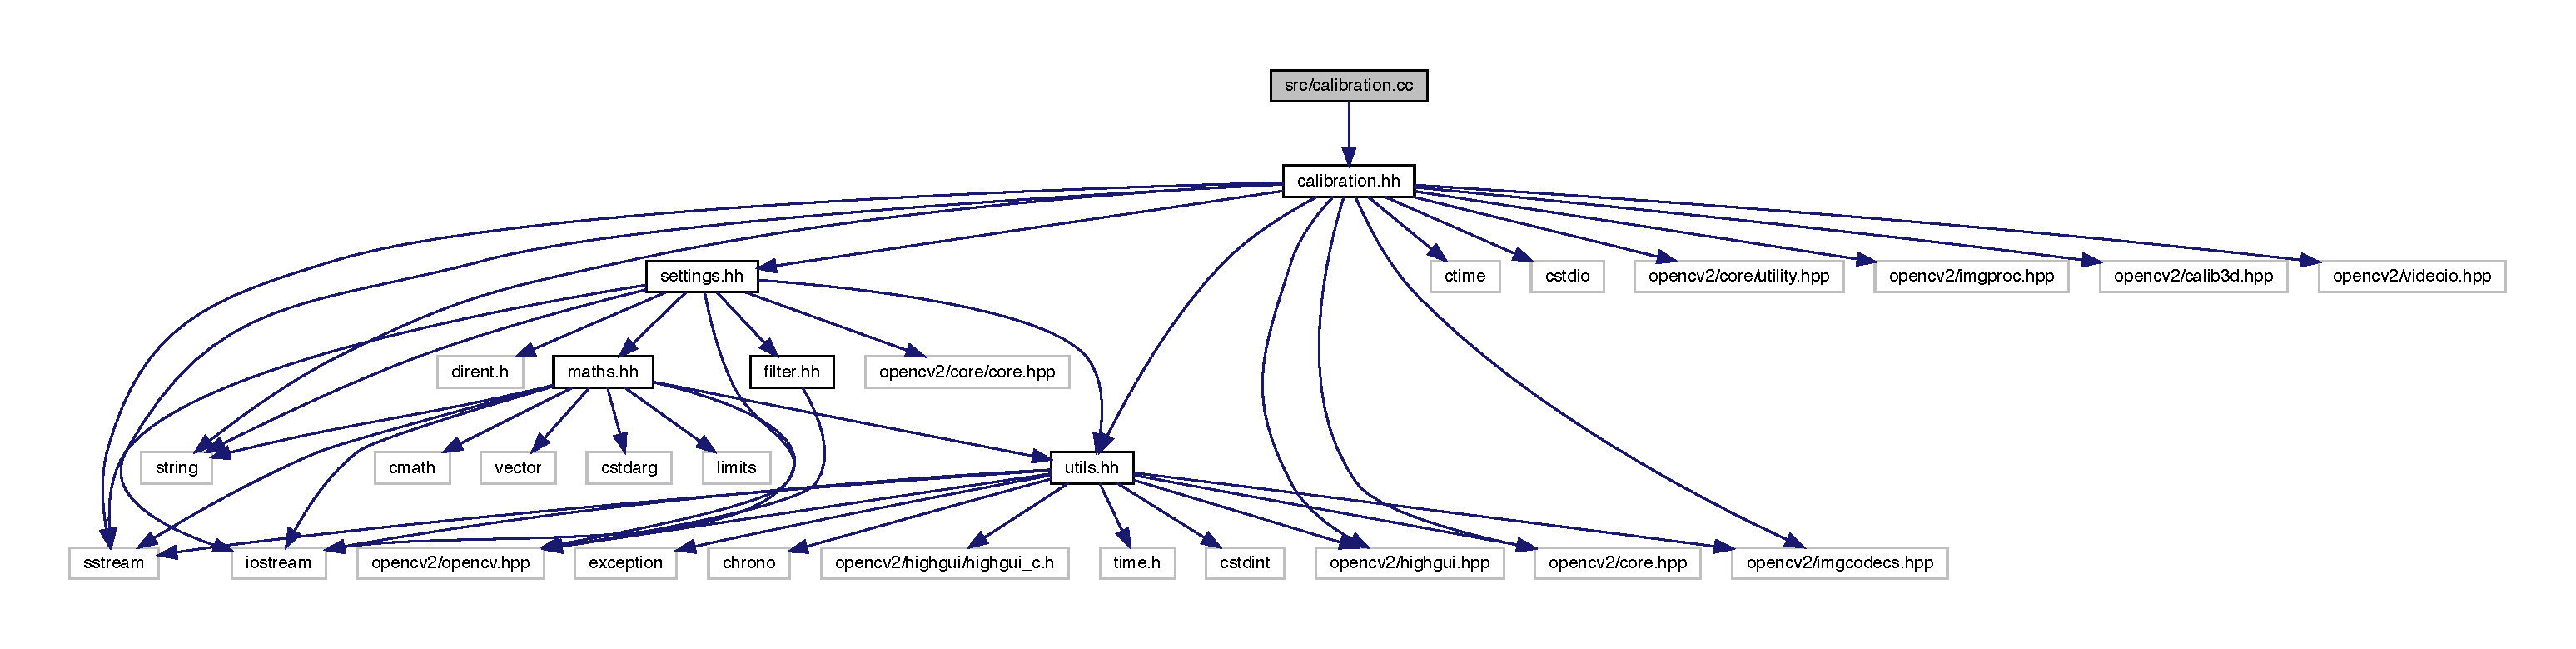
\includegraphics[width=350pt]{calibration_8cc__incl}
\end{center}
\end{figure}
\subsection*{Functions}
\begin{DoxyCompactItemize}
\item 
\mbox{\hyperlink{draw_8hh_aa620a13339ac3a1177c86edc549fda9b}{int}} \mbox{\hyperlink{calibration_8cc_a869b0c5c377f65da8596646d7340d135}{calibration}} (string input\+File)
\begin{DoxyCompactList}\small\item\em Function to run the complete calibration. \end{DoxyCompactList}\item 
static void \mbox{\hyperlink{calibration_8cc_a732d46a8a94e5cc33f89d52dd8395714}{read}} (const File\+Node \&node, \mbox{\hyperlink{class_cal_settings}{Cal\+Settings}} \&x, const \mbox{\hyperlink{class_cal_settings}{Cal\+Settings}} \&default\+\_\+value)
\begin{DoxyCompactList}\small\item\em Reads \mbox{\hyperlink{class_cal_settings}{Cal\+Settings}} from file. If there is none then initiate a new {\ttfamily \mbox{\hyperlink{class_cal_settings}{Cal\+Settings}}}. \end{DoxyCompactList}\item 
static double \mbox{\hyperlink{calibration_8cc_a595849a1b81e38ffd3e1f7f70f88085e}{compute\+Reprojection\+Errors}} (const vector$<$ vector$<$ Point3f $>$ $>$ \&object\+Points, const vector$<$ vector$<$ Point2f $>$ $>$ \&image\+Points, const vector$<$ Mat $>$ \&rvecs, const vector$<$ Mat $>$ \&tvecs, const Mat \&camera\+Matrix, const Mat \&dist\+Coeffs, vector$<$ float $>$ \&per\+View\+Errors, bool fisheye)
\begin{DoxyCompactList}\small\item\em Compute the errors of the projection. \end{DoxyCompactList}\item 
void \mbox{\hyperlink{calibration_8cc_a9deaf00ea7081c5e9ce50a64c9946fa9}{calc\+Board\+Corner\+Positions}} (Size board\+Size, float square\+Size, vector$<$ Point3f $>$ \&corners)
\begin{DoxyCompactList}\small\item\em This function compute the position of the upper corners of every cell. \end{DoxyCompactList}\item 
static bool \mbox{\hyperlink{calibration_8cc_ad985a15627e02f358b321f4d7d47eca1}{run\+Calibration}} (\mbox{\hyperlink{class_cal_settings}{Cal\+Settings}} \&\mbox{\hyperlink{detection_8cc_a9090f9756293390c57567a0bf7630abf}{s}}, Size \&image\+Size, Mat \&camera\+Matrix, Mat \&dist\+Coeffs, vector$<$ vector$<$ Point2f $>$ $>$ image\+Points, vector$<$ Mat $>$ \&rvecs, vector$<$ Mat $>$ \&tvecs, vector$<$ float $>$ \&reproj\+Errs, double \&total\+Avg\+Err)
\begin{DoxyCompactList}\small\item\em This function run the calibration creating the matrixed for the camera and the distorsion coefficients. \end{DoxyCompactList}\item 
static void \mbox{\hyperlink{calibration_8cc_a9a94e87ed45e2dd9c2c5a49b7d01e42f}{save\+Camera\+Params}} (const \mbox{\hyperlink{class_cal_settings}{Cal\+Settings}} \&\mbox{\hyperlink{detection_8cc_a9090f9756293390c57567a0bf7630abf}{s}}, const Size \&image\+Size, const Mat \&camera\+Matrix, const Mat \&dist\+Coeffs, const vector$<$ Mat $>$ \&rvecs, const vector$<$ Mat $>$ \&tvecs, const vector$<$ float $>$ \&reproj\+Errs, const vector$<$ vector$<$ Point2f $>$ $>$ \&image\+Points, const double total\+Avg\+Err)
\begin{DoxyCompactList}\small\item\em Function to save the computed parameters to a file. \end{DoxyCompactList}\item 
bool \mbox{\hyperlink{calibration_8cc_a4195037da024926ac4f645bd09700052}{run\+Calibration\+And\+Save}} (\mbox{\hyperlink{class_cal_settings}{Cal\+Settings}} \&\mbox{\hyperlink{detection_8cc_a9090f9756293390c57567a0bf7630abf}{s}}, Size image\+Size, Mat \&camera\+Matrix, Mat \&dist\+Coeffs, vector$<$ vector$<$ Point2f $>$ $>$ image\+Points)
\begin{DoxyCompactList}\small\item\em Reads \mbox{\hyperlink{class_cal_settings}{Cal\+Settings}} from file. If there is none then initiate a new {\ttfamily \mbox{\hyperlink{class_cal_settings}{Cal\+Settings}}}. \end{DoxyCompactList}\end{DoxyCompactItemize}


\subsection{Function Documentation}
\mbox{\Hypertarget{calibration_8cc_a9deaf00ea7081c5e9ce50a64c9946fa9}\label{calibration_8cc_a9deaf00ea7081c5e9ce50a64c9946fa9}} 
\index{calibration.cc@{calibration.cc}!calcBoardCornerPositions@{calcBoardCornerPositions}}
\index{calcBoardCornerPositions@{calcBoardCornerPositions}!calibration.cc@{calibration.cc}}
\subsubsection{\texorpdfstring{calcBoardCornerPositions()}{calcBoardCornerPositions()}}
{\footnotesize\ttfamily void calc\+Board\+Corner\+Positions (\begin{DoxyParamCaption}\item[{Size}]{board\+Size,  }\item[{float}]{square\+Size,  }\item[{vector$<$ Point3f $>$ \&}]{corners }\end{DoxyParamCaption})}



This function compute the position of the upper corners of every cell. 


\begin{DoxyParams}[1]{Parameters}
\mbox{\texttt{ in}}  & {\em board\+Siz} & The dimension of the chess board. \\
\hline
\mbox{\texttt{ in}}  & {\em square\+Size} & The dimension of the edge of a cell. \\
\hline
\mbox{\texttt{ out}}  & {\em corners} & A vector of Point3fs which equals to the corners of the cells. \\
\hline
\end{DoxyParams}
\mbox{\Hypertarget{calibration_8cc_a869b0c5c377f65da8596646d7340d135}\label{calibration_8cc_a869b0c5c377f65da8596646d7340d135}} 
\index{calibration.cc@{calibration.cc}!calibration@{calibration}}
\index{calibration@{calibration}!calibration.cc@{calibration.cc}}
\subsubsection{\texorpdfstring{calibration()}{calibration()}}
{\footnotesize\ttfamily \mbox{\hyperlink{draw_8hh_aa620a13339ac3a1177c86edc549fda9b}{int}} calibration (\begin{DoxyParamCaption}\item[{string}]{input\+File }\end{DoxyParamCaption})}



Function to run the complete calibration. 


\begin{DoxyParams}[1]{Parameters}
\mbox{\texttt{ in}}  & {\em input\+File} & Name of the setting.\+xml file. It\textquotesingle{}s set to default to default.\+xml\\
\hline
\end{DoxyParams}
\begin{DoxyReturn}{Returns}
-\/2 if the \mbox{\hyperlink{class_cal_settings}{Cal\+Settings}} file could be load but the input was not well-\/formed~\newline
 -\/1 if the \mbox{\hyperlink{class_cal_settings}{Cal\+Settings}} file could not be opened.~\newline
 0 if everything went fine. 
\end{DoxyReturn}
\mbox{\Hypertarget{calibration_8cc_a595849a1b81e38ffd3e1f7f70f88085e}\label{calibration_8cc_a595849a1b81e38ffd3e1f7f70f88085e}} 
\index{calibration.cc@{calibration.cc}!computeReprojectionErrors@{computeReprojectionErrors}}
\index{computeReprojectionErrors@{computeReprojectionErrors}!calibration.cc@{calibration.cc}}
\subsubsection{\texorpdfstring{computeReprojectionErrors()}{computeReprojectionErrors()}}
{\footnotesize\ttfamily static double compute\+Reprojection\+Errors (\begin{DoxyParamCaption}\item[{const vector$<$ vector$<$ Point3f $>$ $>$ \&}]{object\+Points,  }\item[{const vector$<$ vector$<$ Point2f $>$ $>$ \&}]{image\+Points,  }\item[{const vector$<$ Mat $>$ \&}]{rvecs,  }\item[{const vector$<$ Mat $>$ \&}]{tvecs,  }\item[{const Mat \&}]{camera\+Matrix,  }\item[{const Mat \&}]{dist\+Coeffs,  }\item[{vector$<$ float $>$ \&}]{per\+View\+Errors,  }\item[{bool}]{fisheye }\end{DoxyParamCaption})\hspace{0.3cm}{\ttfamily [static]}}



Compute the errors of the projection. 


\begin{DoxyParams}[1]{Parameters}
\mbox{\texttt{ in}}  & {\em object\+Points} & The real image points which will be projected \\
\hline
\mbox{\texttt{ in}}  & {\em rvecs} & Input vector of rotation vectors estimated for each pattern view. \\
\hline
\mbox{\texttt{ in}}  & {\em tvecs} & Input vector of translation vectors estimated for each pattern view. \\
\hline
\mbox{\texttt{ in}}  & {\em camera\+Matrix} & The matrix containing the parameters for the camera \\
\hline
\mbox{\texttt{ in}}  & {\em dist\+Coeffs} & The matrix containing the distortion coefficients. \\
\hline
\mbox{\texttt{ in}}  & {\em fisheye} & A variable which says if a fish eye correction should be applied or no. \\
\hline
\mbox{\texttt{ out}}  & {\em per\+View\+Errors} & A vector containing the error for each image. \\
\hline
\mbox{\texttt{ out}}  & {\em image\+Points} & The projected points for each image.\\
\hline
\end{DoxyParams}
\begin{DoxyReturn}{Returns}
The total error. 
\end{DoxyReturn}
\mbox{\Hypertarget{calibration_8cc_a732d46a8a94e5cc33f89d52dd8395714}\label{calibration_8cc_a732d46a8a94e5cc33f89d52dd8395714}} 
\index{calibration.cc@{calibration.cc}!read@{read}}
\index{read@{read}!calibration.cc@{calibration.cc}}
\subsubsection{\texorpdfstring{read()}{read()}}
{\footnotesize\ttfamily static void read (\begin{DoxyParamCaption}\item[{const File\+Node \&}]{node,  }\item[{\mbox{\hyperlink{class_cal_settings}{Cal\+Settings}} \&}]{x,  }\item[{const \mbox{\hyperlink{class_cal_settings}{Cal\+Settings}} \&}]{default\+\_\+value }\end{DoxyParamCaption})\hspace{0.3cm}{\ttfamily [inline]}, {\ttfamily [static]}}



Reads \mbox{\hyperlink{class_cal_settings}{Cal\+Settings}} from file. If there is none then initiate a new {\ttfamily \mbox{\hyperlink{class_cal_settings}{Cal\+Settings}}}. 


\begin{DoxyParams}[1]{Parameters}
\mbox{\texttt{ in}}  & {\em node} & node to consider for getting \mbox{\hyperlink{class_cal_settings}{Cal\+Settings}}; \\
\hline
\mbox{\texttt{ in}}  & {\em x} & {\ttfamily \mbox{\hyperlink{class_cal_settings}{Cal\+Settings}}} to configure; \\
\hline
\mbox{\texttt{ in}}  & {\em default\+\_\+value} & {\ttfamily \mbox{\hyperlink{class_cal_settings}{Cal\+Settings}}} default value. Setted to {\ttfamily \mbox{\hyperlink{class_cal_settings}{Cal\+Settings()}}}. \\
\hline
\end{DoxyParams}
\mbox{\Hypertarget{calibration_8cc_ad985a15627e02f358b321f4d7d47eca1}\label{calibration_8cc_ad985a15627e02f358b321f4d7d47eca1}} 
\index{calibration.cc@{calibration.cc}!runCalibration@{runCalibration}}
\index{runCalibration@{runCalibration}!calibration.cc@{calibration.cc}}
\subsubsection{\texorpdfstring{runCalibration()}{runCalibration()}}
{\footnotesize\ttfamily static bool run\+Calibration (\begin{DoxyParamCaption}\item[{\mbox{\hyperlink{class_cal_settings}{Cal\+Settings}} \&}]{s,  }\item[{Size \&}]{image\+Size,  }\item[{Mat \&}]{camera\+Matrix,  }\item[{Mat \&}]{dist\+Coeffs,  }\item[{vector$<$ vector$<$ Point2f $>$ $>$}]{image\+Points,  }\item[{vector$<$ Mat $>$ \&}]{rvecs,  }\item[{vector$<$ Mat $>$ \&}]{tvecs,  }\item[{vector$<$ float $>$ \&}]{reproj\+Errs,  }\item[{double \&}]{total\+Avg\+Err }\end{DoxyParamCaption})\hspace{0.3cm}{\ttfamily [static]}}



This function run the calibration creating the matrixed for the camera and the distorsion coefficients. 


\begin{DoxyParams}[1]{Parameters}
\mbox{\texttt{ in}}  & {\em s} & The {\ttfamily \mbox{\hyperlink{class_cal_settings}{Cal\+Settings}}} read from the file and memorized. \\
\hline
\mbox{\texttt{ in}}  & {\em image\+Size} & The size of the image used in {\ttfamily calibrate\+Camera()} to initialize the camera matrix. \\
\hline
\mbox{\texttt{ in}}  & {\em image\+Points} & The projected points for each image. \\
\hline
\mbox{\texttt{ in}}  & {\em reproj\+Errs} & The re-\/projection error, that is a geometric error corresponding to the image distance between a projected point and a measured one. \\
\hline
\mbox{\texttt{ out}}  & {\em camera\+Matrix} & The matrix of the camera parameters \\
\hline
\mbox{\texttt{ out}}  & {\em dist\+Coeffs} & The matrix of the distorsion coefficients. \\
\hline
\mbox{\texttt{ out}}  & {\em rvecs} & Output vector of rotation vectors estimated for each pattern view. \\
\hline
\mbox{\texttt{ out}}  & {\em tvecs} & Output vector of translation vectors estimated for each pattern view. \\
\hline
\mbox{\texttt{ out}}  & {\em total\+Avg\+Err} & The total avarage error given from distorsion.\\
\hline
\end{DoxyParams}
\begin{DoxyReturn}{Returns}
{\ttfamily false} if one or more elements in the {\ttfamily camera\+Matrix} and {\ttfamily dist\+Coeffs} are invalid.~\newline
 {\ttfamily true} if all the elements are valid. 
\end{DoxyReturn}
\mbox{\Hypertarget{calibration_8cc_a4195037da024926ac4f645bd09700052}\label{calibration_8cc_a4195037da024926ac4f645bd09700052}} 
\index{calibration.cc@{calibration.cc}!runCalibrationAndSave@{runCalibrationAndSave}}
\index{runCalibrationAndSave@{runCalibrationAndSave}!calibration.cc@{calibration.cc}}
\subsubsection{\texorpdfstring{runCalibrationAndSave()}{runCalibrationAndSave()}}
{\footnotesize\ttfamily bool run\+Calibration\+And\+Save (\begin{DoxyParamCaption}\item[{\mbox{\hyperlink{class_cal_settings}{Cal\+Settings}} \&}]{s,  }\item[{Size}]{image\+Size,  }\item[{Mat \&}]{camera\+Matrix,  }\item[{Mat \&}]{dist\+Coeffs,  }\item[{vector$<$ vector$<$ Point2f $>$ $>$}]{image\+Points }\end{DoxyParamCaption})}



Reads \mbox{\hyperlink{class_cal_settings}{Cal\+Settings}} from file. If there is none then initiate a new {\ttfamily \mbox{\hyperlink{class_cal_settings}{Cal\+Settings}}}. 


\begin{DoxyParams}[1]{Parameters}
\mbox{\texttt{ in}}  & {\em s} & The {\ttfamily \mbox{\hyperlink{class_cal_settings}{Cal\+Settings}}} being used during the execution. \\
\hline
\mbox{\texttt{ in}}  & {\em image\+Size} & The dimensions of the images. \\
\hline
\mbox{\texttt{ in}}  & {\em image\+Points} & The projected points for each image. \\
\hline
\mbox{\texttt{ out}}  & {\em camera\+Matrix} & The matrix which is used to store the values for the camera parameters. \\
\hline
\mbox{\texttt{ out}}  & {\em dist\+Coeffs} & The matrix which is used to store the distortion coefficients.\\
\hline
\end{DoxyParams}
\begin{DoxyReturn}{Returns}
{\ttfamily true} if the calibration succeded.~\newline
 {\ttfamily false} otherwise. 
\end{DoxyReturn}
\mbox{\Hypertarget{calibration_8cc_a9a94e87ed45e2dd9c2c5a49b7d01e42f}\label{calibration_8cc_a9a94e87ed45e2dd9c2c5a49b7d01e42f}} 
\index{calibration.cc@{calibration.cc}!saveCameraParams@{saveCameraParams}}
\index{saveCameraParams@{saveCameraParams}!calibration.cc@{calibration.cc}}
\subsubsection{\texorpdfstring{saveCameraParams()}{saveCameraParams()}}
{\footnotesize\ttfamily static void save\+Camera\+Params (\begin{DoxyParamCaption}\item[{const \mbox{\hyperlink{class_cal_settings}{Cal\+Settings}} \&}]{s,  }\item[{const Size \&}]{image\+Size,  }\item[{const Mat \&}]{camera\+Matrix,  }\item[{const Mat \&}]{dist\+Coeffs,  }\item[{const vector$<$ Mat $>$ \&}]{rvecs,  }\item[{const vector$<$ Mat $>$ \&}]{tvecs,  }\item[{const vector$<$ float $>$ \&}]{reproj\+Errs,  }\item[{const vector$<$ vector$<$ Point2f $>$ $>$ \&}]{image\+Points,  }\item[{const double}]{total\+Avg\+Err }\end{DoxyParamCaption})\hspace{0.3cm}{\ttfamily [static]}}



Function to save the computed parameters to a file. 


\begin{DoxyParams}[1]{Parameters}
\mbox{\texttt{ in}}  & {\em s} & Use the {\ttfamily \mbox{\hyperlink{class_cal_settings}{Cal\+Settings}}} got at the beginning for information as the output file name, image and board size. \\
\hline
\mbox{\texttt{ in}}  & {\em image\+Size} & The size of the imgage. \\
\hline
\mbox{\texttt{ in}}  & {\em camera\+Matrix} & The camera matrix. \\
\hline
\mbox{\texttt{ in}}  & {\em dist\+Coeffs} & The distorsion coefficient matrix. \\
\hline
 & {\em \mbox{[}int\mbox{]}} & rvecs Vector of rotation vectors estimated for each pattern view. \\
\hline
\mbox{\texttt{ in}}  & {\em tvecs} & Vector of translation vectors estimated for each pattern view. \\
\hline
\mbox{\texttt{ in}}  & {\em reproj\+Errs} & The re-\/projection error, that is a geometric error corresponding to the image distance between a projected point and a measured one. \\
\hline
\mbox{\texttt{ in}}  & {\em image\+Points} & The projected points for each image. \\
\hline
\mbox{\texttt{ in}}  & {\em total\+Avg\+Err} & The total avarage error given from distorsion. \\
\hline
\end{DoxyParams}
Open file for writing

Stores time of calibration

Store infos about the images 
\hypertarget{calibration_8hh}{}\section{src/calibration.hh File Reference}
\label{calibration_8hh}\index{src/calibration.\+hh@{src/calibration.\+hh}}


Library for calibration.  


{\ttfamily \#include \char`\"{}utils.\+hh\char`\"{}}\newline
{\ttfamily \#include $<$iostream$>$}\newline
{\ttfamily \#include $<$sstream$>$}\newline
{\ttfamily \#include $<$string$>$}\newline
{\ttfamily \#include $<$ctime$>$}\newline
{\ttfamily \#include $<$cstdio$>$}\newline
{\ttfamily \#include $<$opencv2/core.\+hpp$>$}\newline
{\ttfamily \#include $<$opencv2/core/utility.\+hpp$>$}\newline
{\ttfamily \#include $<$opencv2/imgproc.\+hpp$>$}\newline
{\ttfamily \#include $<$opencv2/calib3d.\+hpp$>$}\newline
{\ttfamily \#include $<$opencv2/imgcodecs.\+hpp$>$}\newline
{\ttfamily \#include $<$opencv2/videoio.\+hpp$>$}\newline
{\ttfamily \#include $<$opencv2/highgui.\+hpp$>$}\newline
Include dependency graph for calibration.\+hh\+:
\nopagebreak
\begin{figure}[H]
\begin{center}
\leavevmode
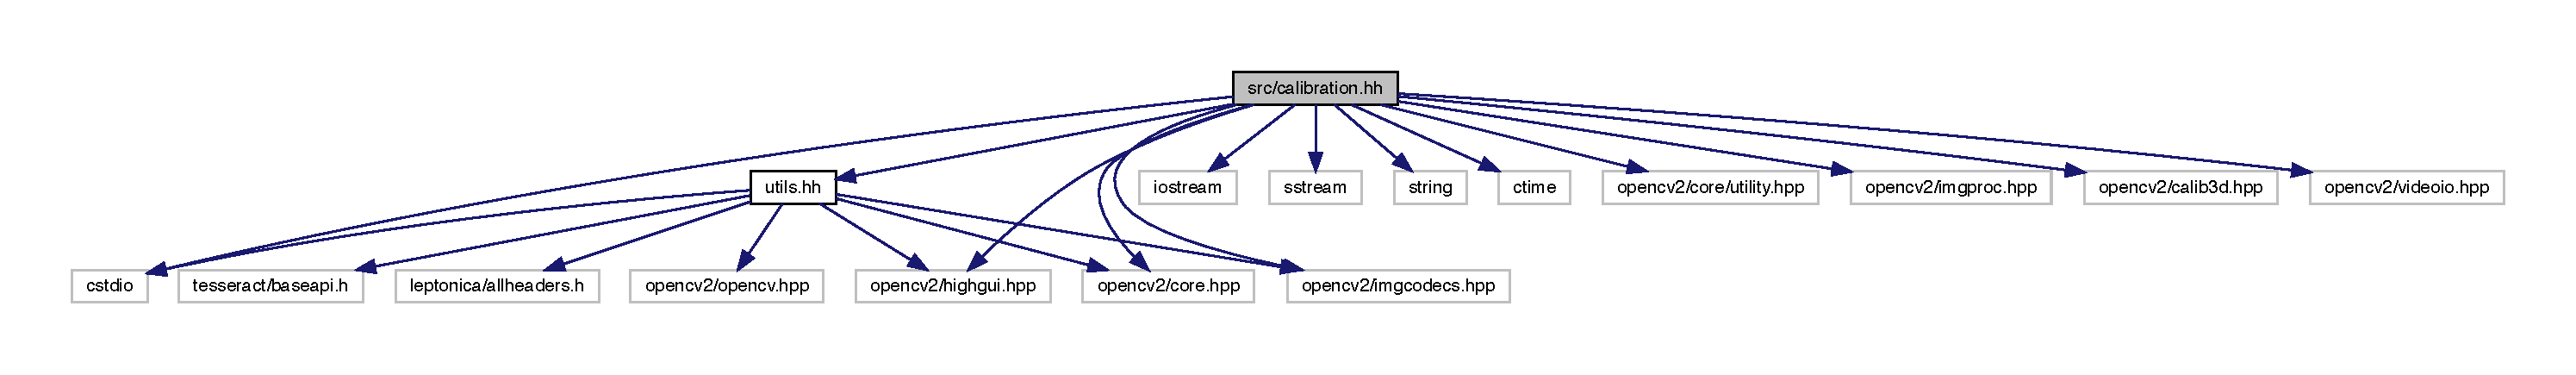
\includegraphics[width=350pt]{calibration_8hh__incl}
\end{center}
\end{figure}
This graph shows which files directly or indirectly include this file\+:
\nopagebreak
\begin{figure}[H]
\begin{center}
\leavevmode
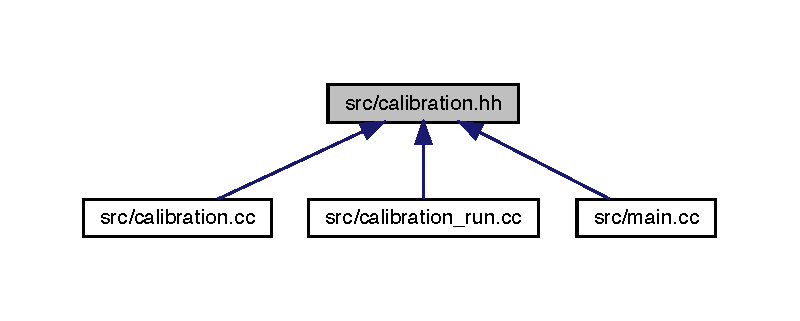
\includegraphics[width=350pt]{calibration_8hh__dep__incl}
\end{center}
\end{figure}
\subsection*{Classes}
\begin{DoxyCompactItemize}
\item 
class \mbox{\hyperlink{class_settings}{Settings}}
\end{DoxyCompactItemize}
\subsection*{Enumerations}
\begin{DoxyCompactItemize}
\item 
enum \{ \mbox{\hyperlink{calibration_8hh_a06fc87d81c62e9abb8790b6e5713c55ba167a7ee1aabe9f27e010fff93c0ba971}{D\+E\+T\+E\+C\+T\+I\+ON}} = 0, 
\mbox{\hyperlink{calibration_8hh_a06fc87d81c62e9abb8790b6e5713c55ba53f5d985011ab26db21516188f46a94f}{C\+A\+P\+T\+U\+R\+I\+NG}} = 1, 
\mbox{\hyperlink{calibration_8hh_a06fc87d81c62e9abb8790b6e5713c55baf7834eaf5a327e180e039aa05dd3ebd1}{C\+A\+L\+I\+B\+R\+A\+T\+ED}} = 2
 \}
\end{DoxyCompactItemize}
\subsection*{Functions}
\begin{DoxyCompactItemize}
\item 
int \mbox{\hyperlink{calibration_8hh_a9deafd96b6adbc102c47af08cde6610c}{calibration}} (const string input\+File=\char`\"{}data/calib\+\_\+config.\+xml\char`\"{})
\begin{DoxyCompactList}\small\item\em Function to run the complete calibration. \end{DoxyCompactList}\item 
bool \mbox{\hyperlink{calibration_8hh_ac7558c8da6af683fc1c86c2ede7bb31c}{run\+Calibration\+And\+Save}} (\mbox{\hyperlink{class_settings}{Settings}} \&s, Size image\+Size, Mat \&camera\+Matrix, Mat \&dist\+Coeffs, vector$<$ vector$<$ Point2f $>$ $>$ image\+Points)
\begin{DoxyCompactList}\small\item\em Reads settings from file. If there is none then initiate a new {\ttfamily \mbox{\hyperlink{class_settings}{Settings}}}. \end{DoxyCompactList}\end{DoxyCompactItemize}


\subsection{Detailed Description}
Library for calibration. 



\subsection{Enumeration Type Documentation}
\mbox{\Hypertarget{calibration_8hh_a06fc87d81c62e9abb8790b6e5713c55b}\label{calibration_8hh_a06fc87d81c62e9abb8790b6e5713c55b}} 
\subsubsection{\texorpdfstring{anonymous enum}{anonymous enum}}
{\footnotesize\ttfamily anonymous enum}

\begin{DoxyEnumFields}{Enumerator}
\raisebox{\heightof{T}}[0pt][0pt]{\index{D\+E\+T\+E\+C\+T\+I\+ON@{D\+E\+T\+E\+C\+T\+I\+ON}!calibration.\+hh@{calibration.\+hh}}\index{calibration.\+hh@{calibration.\+hh}!D\+E\+T\+E\+C\+T\+I\+ON@{D\+E\+T\+E\+C\+T\+I\+ON}}}\mbox{\Hypertarget{calibration_8hh_a06fc87d81c62e9abb8790b6e5713c55ba167a7ee1aabe9f27e010fff93c0ba971}\label{calibration_8hh_a06fc87d81c62e9abb8790b6e5713c55ba167a7ee1aabe9f27e010fff93c0ba971}} 
D\+E\+T\+E\+C\+T\+I\+ON&\\
\hline

\raisebox{\heightof{T}}[0pt][0pt]{\index{C\+A\+P\+T\+U\+R\+I\+NG@{C\+A\+P\+T\+U\+R\+I\+NG}!calibration.\+hh@{calibration.\+hh}}\index{calibration.\+hh@{calibration.\+hh}!C\+A\+P\+T\+U\+R\+I\+NG@{C\+A\+P\+T\+U\+R\+I\+NG}}}\mbox{\Hypertarget{calibration_8hh_a06fc87d81c62e9abb8790b6e5713c55ba53f5d985011ab26db21516188f46a94f}\label{calibration_8hh_a06fc87d81c62e9abb8790b6e5713c55ba53f5d985011ab26db21516188f46a94f}} 
C\+A\+P\+T\+U\+R\+I\+NG&\\
\hline

\raisebox{\heightof{T}}[0pt][0pt]{\index{C\+A\+L\+I\+B\+R\+A\+T\+ED@{C\+A\+L\+I\+B\+R\+A\+T\+ED}!calibration.\+hh@{calibration.\+hh}}\index{calibration.\+hh@{calibration.\+hh}!C\+A\+L\+I\+B\+R\+A\+T\+ED@{C\+A\+L\+I\+B\+R\+A\+T\+ED}}}\mbox{\Hypertarget{calibration_8hh_a06fc87d81c62e9abb8790b6e5713c55baf7834eaf5a327e180e039aa05dd3ebd1}\label{calibration_8hh_a06fc87d81c62e9abb8790b6e5713c55baf7834eaf5a327e180e039aa05dd3ebd1}} 
C\+A\+L\+I\+B\+R\+A\+T\+ED&\\
\hline

\end{DoxyEnumFields}


\subsection{Function Documentation}
\mbox{\Hypertarget{calibration_8hh_a9deafd96b6adbc102c47af08cde6610c}\label{calibration_8hh_a9deafd96b6adbc102c47af08cde6610c}} 
\index{calibration.\+hh@{calibration.\+hh}!calibration@{calibration}}
\index{calibration@{calibration}!calibration.\+hh@{calibration.\+hh}}
\subsubsection{\texorpdfstring{calibration()}{calibration()}}
{\footnotesize\ttfamily int calibration (\begin{DoxyParamCaption}\item[{const string}]{input\+File }\end{DoxyParamCaption})}



Function to run the complete calibration. 


\begin{DoxyParams}[1]{Parameters}
\mbox{\tt in}  & {\em input\+File} & Name of the setting.\+xml file. It\textquotesingle{}s set to default to default.\+xml\\
\hline
\end{DoxyParams}
\begin{DoxyReturn}{Returns}
-\/2 if the settings file could be load but the input was not well-\/formed~\newline
 -\/1 if the settings file could not be opened.~\newline
 0 if everything went fine. 
\end{DoxyReturn}
\mbox{\Hypertarget{calibration_8hh_ac7558c8da6af683fc1c86c2ede7bb31c}\label{calibration_8hh_ac7558c8da6af683fc1c86c2ede7bb31c}} 
\index{calibration.\+hh@{calibration.\+hh}!run\+Calibration\+And\+Save@{run\+Calibration\+And\+Save}}
\index{run\+Calibration\+And\+Save@{run\+Calibration\+And\+Save}!calibration.\+hh@{calibration.\+hh}}
\subsubsection{\texorpdfstring{run\+Calibration\+And\+Save()}{runCalibrationAndSave()}}
{\footnotesize\ttfamily bool run\+Calibration\+And\+Save (\begin{DoxyParamCaption}\item[{\mbox{\hyperlink{class_settings}{Settings}} \&}]{s,  }\item[{Size}]{image\+Size,  }\item[{Mat \&}]{camera\+Matrix,  }\item[{Mat \&}]{dist\+Coeffs,  }\item[{vector$<$ vector$<$ Point2f $>$ $>$}]{image\+Points }\end{DoxyParamCaption})}



Reads settings from file. If there is none then initiate a new {\ttfamily \mbox{\hyperlink{class_settings}{Settings}}}. 


\begin{DoxyParams}[1]{Parameters}
\mbox{\tt in}  & {\em s} & The {\ttfamily \mbox{\hyperlink{class_settings}{Settings}}} being used during the execution. \\
\hline
\mbox{\tt in}  & {\em image\+Size} & The dimensions of the images. \\
\hline
\mbox{\tt in}  & {\em image\+Points} & The projected points for each image. \\
\hline
\mbox{\tt out}  & {\em camera\+Matrix} & The matrix which is used to store the values for the camera parameters. \\
\hline
\mbox{\tt out}  & {\em dist\+Coeffs} & The matrix which is used to store the distortion coefficients.\\
\hline
\end{DoxyParams}
\begin{DoxyReturn}{Returns}
{\ttfamily true} if the calibration succeded.~\newline
 {\ttfamily false} otherwise. 
\end{DoxyReturn}

\hypertarget{calibration__run_8cc}{}\section{src/calibration\+\_\+run.cc File Reference}
\label{calibration__run_8cc}\index{src/calibration\+\_\+run.\+cc@{src/calibration\+\_\+run.\+cc}}
{\ttfamily \#include \char`\"{}calibration.\+hh\char`\"{}}\newline
Include dependency graph for calibration\+\_\+run.\+cc\+:
\nopagebreak
\begin{figure}[H]
\begin{center}
\leavevmode
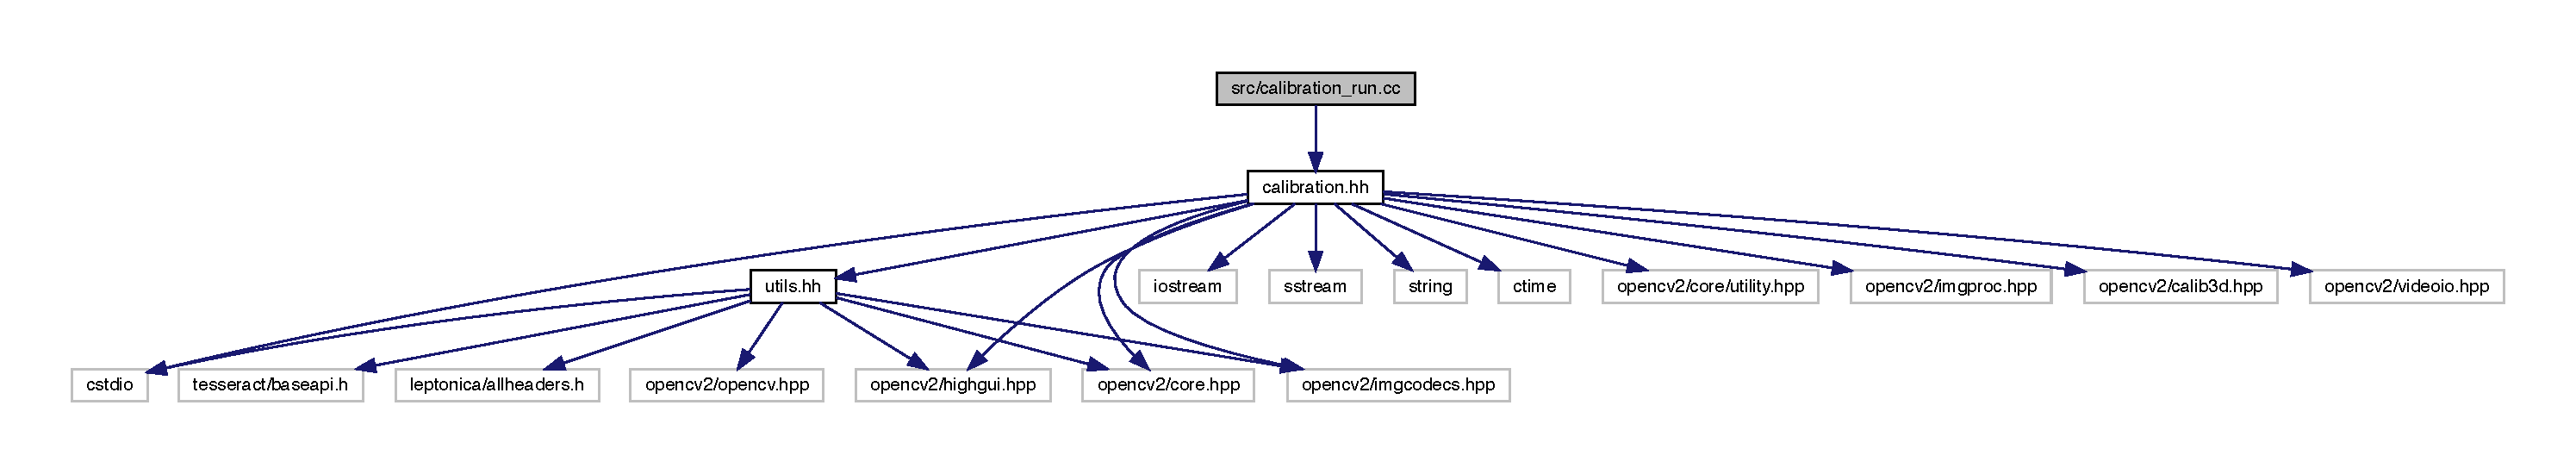
\includegraphics[width=350pt]{calibration__run_8cc__incl}
\end{center}
\end{figure}
\subsection*{Functions}
\begin{DoxyCompactItemize}
\item 
int \mbox{\hyperlink{calibration__run_8cc_ae66f6b31b5ad750f1fe042a706a4e3d4}{main}} ()
\end{DoxyCompactItemize}


\subsection{Function Documentation}
\mbox{\Hypertarget{calibration__run_8cc_ae66f6b31b5ad750f1fe042a706a4e3d4}\label{calibration__run_8cc_ae66f6b31b5ad750f1fe042a706a4e3d4}} 
\index{calibration\+\_\+run.\+cc@{calibration\+\_\+run.\+cc}!main@{main}}
\index{main@{main}!calibration\+\_\+run.\+cc@{calibration\+\_\+run.\+cc}}
\subsubsection{\texorpdfstring{main()}{main()}}
{\footnotesize\ttfamily int main (\begin{DoxyParamCaption}{ }\end{DoxyParamCaption})}


\hypertarget{create__xml_8cc}{}\section{src/create\+\_\+xml.cc File Reference}
\label{create__xml_8cc}\index{src/create\+\_\+xml.\+cc@{src/create\+\_\+xml.\+cc}}
{\ttfamily \#include $<$opencv2/core/core.\+hpp$>$}\newline
{\ttfamily \#include $<$iostream$>$}\newline
{\ttfamily \#include $<$string$>$}\newline
Include dependency graph for create\+\_\+xml.\+cc\+:
\nopagebreak
\begin{figure}[H]
\begin{center}
\leavevmode
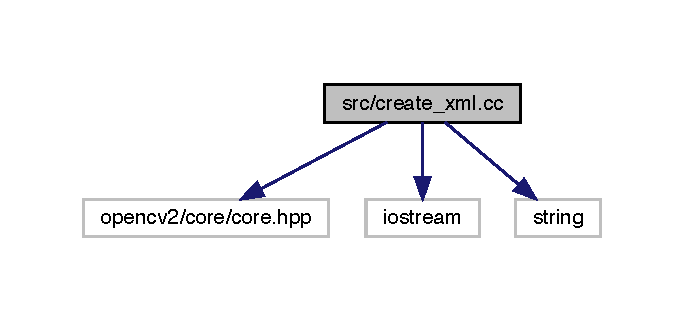
\includegraphics[width=328pt]{create__xml_8cc__incl}
\end{center}
\end{figure}
\subsection*{Functions}
\begin{DoxyCompactItemize}
\item 
int \mbox{\hyperlink{create__xml_8cc_ae66f6b31b5ad750f1fe042a706a4e3d4}{main}} ()
\end{DoxyCompactItemize}


\subsection{Function Documentation}
\mbox{\Hypertarget{create__xml_8cc_ae66f6b31b5ad750f1fe042a706a4e3d4}\label{create__xml_8cc_ae66f6b31b5ad750f1fe042a706a4e3d4}} 
\index{create\+\_\+xml.\+cc@{create\+\_\+xml.\+cc}!main@{main}}
\index{main@{main}!create\+\_\+xml.\+cc@{create\+\_\+xml.\+cc}}
\subsubsection{\texorpdfstring{main()}{main()}}
{\footnotesize\ttfamily int main (\begin{DoxyParamCaption}{ }\end{DoxyParamCaption})}


\hypertarget{detection_8cc}{}\section{src/detection.cc File Reference}
\label{detection_8cc}\index{src/detection.cc@{src/detection.cc}}
{\ttfamily \#include \char`\"{}detection.\+hh\char`\"{}}\newline
Include dependency graph for detection.\+cc\+:
\nopagebreak
\begin{figure}[H]
\begin{center}
\leavevmode
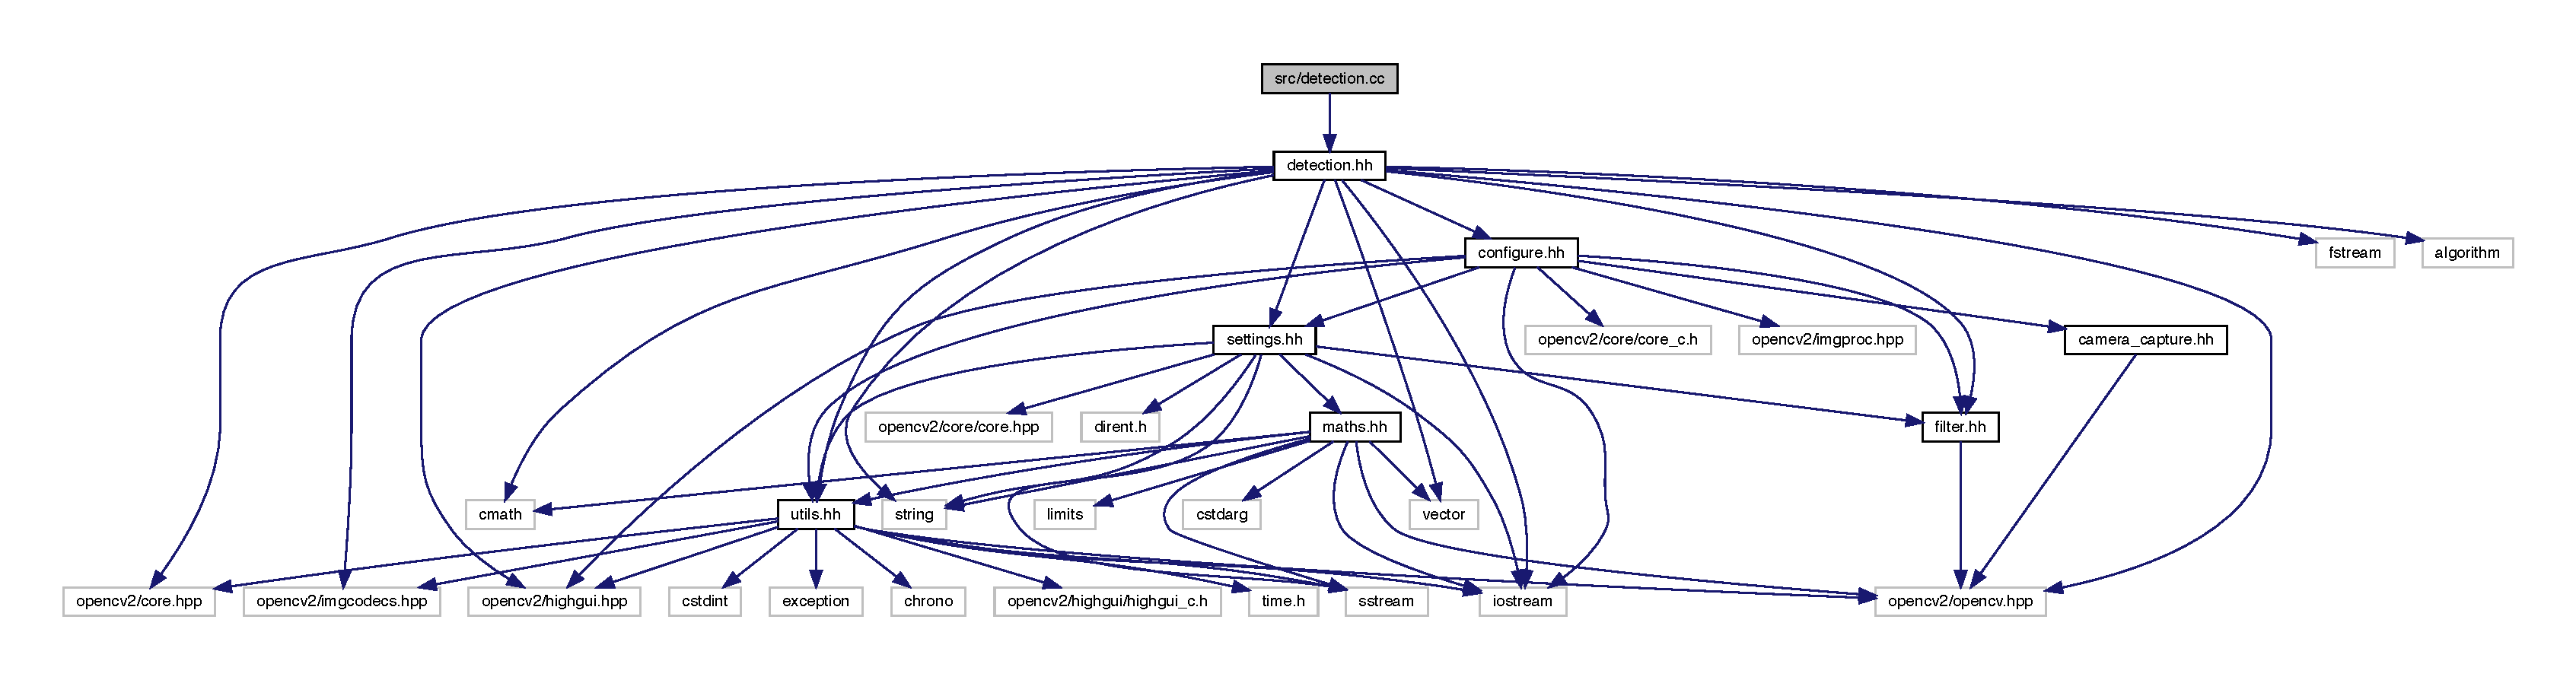
\includegraphics[width=350pt]{detection_8cc__incl}
\end{center}
\end{figure}
\subsection*{Macros}
\begin{DoxyCompactItemize}
\item 
\#define \mbox{\hyperlink{detection_8cc_a0cfe53ea953c48d0949ffb63574ccd3b}{E\+P\+S\+\_\+\+C\+U\+R\+VE}}~3
\begin{DoxyCompactList}\small\item\em Given an image, in black/white format, identify all the borders that delimit the shapes. \end{DoxyCompactList}\end{DoxyCompactItemize}
\subsection*{Functions}
\begin{DoxyCompactItemize}
\item 
\mbox{\hyperlink{draw_8hh_aa620a13339ac3a1177c86edc549fda9b}{int}} \mbox{\hyperlink{detection_8cc_a17e13c447692201697b084a1906cf6fb}{detection}} ()
\begin{DoxyCompactList}\small\item\em Loads some images and detects shapes according to different colors. \end{DoxyCompactList}\item 
void \mbox{\hyperlink{detection_8cc_a50993b0aa4f01d89a4e5d0aef4e1e5f4}{load\+\_\+number\+\_\+template}} ()
\begin{DoxyCompactList}\small\item\em Load some templates and save them in the global variable \textquotesingle{}templates\textquotesingle{}. \end{DoxyCompactList}\item 
void \mbox{\hyperlink{detection_8cc_ac47563337453ac7d1314fe83218c87fc}{shape\+\_\+detection}} (const Mat \&img, const \mbox{\hyperlink{draw_8hh_aa620a13339ac3a1177c86edc549fda9b}{int}} color, const Mat \&un\+\_\+img)
\begin{DoxyCompactList}\small\item\em Detect shapes inside the image according to the variable \textquotesingle{}color\textquotesingle{}. \end{DoxyCompactList}\item 
void \mbox{\hyperlink{detection_8cc_a28d0cdb56cfb2164f939dc2f83d1d9d0}{erode\+\_\+dilation}} (Mat \&img, const \mbox{\hyperlink{draw_8hh_aa620a13339ac3a1177c86edc549fda9b}{int}} color)
\begin{DoxyCompactList}\small\item\em It apply some filtering function for isolate the subject and remove the noise. \end{DoxyCompactList}\item 
void \mbox{\hyperlink{detection_8cc_a93844a9ac3d8be0bd871bb41f8260330}{find\+\_\+contours}} (const Mat \&img, Mat original, const \mbox{\hyperlink{draw_8hh_aa620a13339ac3a1177c86edc549fda9b}{int}} color)
\begin{DoxyCompactList}\small\item\em Given an image, in black/white format, identify all the borders that delimit the shapes. \end{DoxyCompactList}\item 
void \mbox{\hyperlink{detection_8cc_a923b178671e2272c6b082335d118716a}{save\+\_\+convex\+\_\+hull}} (const vector$<$ vector$<$ Point $>$$>$ \&contours, const \mbox{\hyperlink{draw_8hh_aa620a13339ac3a1177c86edc549fda9b}{int}} color, const vector$<$ \mbox{\hyperlink{draw_8hh_aa620a13339ac3a1177c86edc549fda9b}{int}} $>$ \&victims)
\begin{DoxyCompactList}\small\item\em Given some vector save it in a xml file. \end{DoxyCompactList}\item 
\mbox{\hyperlink{draw_8hh_aa620a13339ac3a1177c86edc549fda9b}{int}} \mbox{\hyperlink{detection_8cc_a785fcf35ca81d113a1ea3d831fbdbc22}{number\+\_\+recognition}} (Rect blob, const Mat \&base)
\begin{DoxyCompactList}\small\item\em Detect a number on an image inside a region of interest. \end{DoxyCompactList}\item 
void \mbox{\hyperlink{detection_8cc_a2a7fdd973151b59a6b324eaf4f70fdfe}{crop\+\_\+number\+\_\+section}} (Mat \&R\+OI)
\begin{DoxyCompactList}\small\item\em Given an image identify the region of interest(\+R\+O\+I) and crop it out. \end{DoxyCompactList}\end{DoxyCompactItemize}
\subsection*{Variables}
\begin{DoxyCompactItemize}
\item 
vector$<$ Mat $>$ \mbox{\hyperlink{detection_8cc_ad6ec2d6b7fce088fa5e9f335f9a6ed38}{templates}}
\item 
\mbox{\hyperlink{class_settings}{Settings}} $\ast$ \mbox{\hyperlink{detection_8cc_a9090f9756293390c57567a0bf7630abf}{s}} =new \mbox{\hyperlink{class_settings}{Settings}}
\end{DoxyCompactItemize}


\subsection{Macro Definition Documentation}
\mbox{\Hypertarget{detection_8cc_a0cfe53ea953c48d0949ffb63574ccd3b}\label{detection_8cc_a0cfe53ea953c48d0949ffb63574ccd3b}} 
\index{detection.cc@{detection.cc}!EPS\_CURVE@{EPS\_CURVE}}
\index{EPS\_CURVE@{EPS\_CURVE}!detection.cc@{detection.cc}}
\subsubsection{\texorpdfstring{EPS\_CURVE}{EPS\_CURVE}}
{\footnotesize\ttfamily \#define E\+P\+S\+\_\+\+C\+U\+R\+VE~3}



Given an image, in black/white format, identify all the borders that delimit the shapes. 


\begin{DoxyParams}[1]{Parameters}
\mbox{\texttt{ in}}  & {\em img} & Is an image in H\+SV format at the base of the elaboration process. \\
\hline
\mbox{\texttt{ out}}  & {\em original} & Is the original source of \textquotesingle{}img\textquotesingle{}, it is used for showing the detected contours. \\
\hline
\mbox{\texttt{ in}}  & {\em color} & Can has 3 value\+:~\newline
0 -\/$>$ Red~\newline
1 -\/$>$ Green~\newline
2 -\/$>$ Blue~\newline
Is used for decid which procedure apply to the image. \\
\hline
\end{DoxyParams}


\subsection{Function Documentation}
\mbox{\Hypertarget{detection_8cc_a2a7fdd973151b59a6b324eaf4f70fdfe}\label{detection_8cc_a2a7fdd973151b59a6b324eaf4f70fdfe}} 
\index{detection.cc@{detection.cc}!crop\_number\_section@{crop\_number\_section}}
\index{crop\_number\_section@{crop\_number\_section}!detection.cc@{detection.cc}}
\subsubsection{\texorpdfstring{crop\_number\_section()}{crop\_number\_section()}}
{\footnotesize\ttfamily void crop\+\_\+number\+\_\+section (\begin{DoxyParamCaption}\item[{Mat \&}]{R\+OI }\end{DoxyParamCaption})}



Given an image identify the region of interest(\+R\+O\+I) and crop it out. 


\begin{DoxyParams}[1]{Parameters}
\mbox{\texttt{ in,out}}  & {\em R\+OI} & Is the image that the function will going to elaborate. \\
\hline
\end{DoxyParams}
\mbox{\Hypertarget{detection_8cc_a17e13c447692201697b084a1906cf6fb}\label{detection_8cc_a17e13c447692201697b084a1906cf6fb}} 
\index{detection.cc@{detection.cc}!detection@{detection}}
\index{detection@{detection}!detection.cc@{detection.cc}}
\subsubsection{\texorpdfstring{detection()}{detection()}}
{\footnotesize\ttfamily \mbox{\hyperlink{draw_8hh_aa620a13339ac3a1177c86edc549fda9b}{int}} detection (\begin{DoxyParamCaption}{ }\end{DoxyParamCaption})}



Loads some images and detects shapes according to different colors. 

\begin{DoxyReturn}{Returns}
Return 0 if the function reach the end. 
\end{DoxyReturn}
\mbox{\Hypertarget{detection_8cc_a28d0cdb56cfb2164f939dc2f83d1d9d0}\label{detection_8cc_a28d0cdb56cfb2164f939dc2f83d1d9d0}} 
\index{detection.cc@{detection.cc}!erode\_dilation@{erode\_dilation}}
\index{erode\_dilation@{erode\_dilation}!detection.cc@{detection.cc}}
\subsubsection{\texorpdfstring{erode\_dilation()}{erode\_dilation()}}
{\footnotesize\ttfamily void erode\+\_\+dilation (\begin{DoxyParamCaption}\item[{Mat \&}]{img,  }\item[{const \mbox{\hyperlink{draw_8hh_aa620a13339ac3a1177c86edc549fda9b}{int}}}]{color }\end{DoxyParamCaption})}



It apply some filtering function for isolate the subject and remove the noise. 

An example of the sub functions called are\+: Gaussian\+Blur, Erosion, Dilation and Threshold.


\begin{DoxyParams}[1]{Parameters}
\mbox{\texttt{ in,out}}  & {\em img} & Is the image on which the function apply the filtering. \\
\hline
\mbox{\texttt{ in}}  & {\em color} & Can has 4 value\+:~\newline
0 -\/$>$ Red~\newline
1 -\/$>$ Green~\newline
2 -\/$>$ Blue~\newline
3 -\/$>$ Black~\newline
According to the color the filtering functions apply can change in the type and in the order. \\
\hline
\end{DoxyParams}
\mbox{\Hypertarget{detection_8cc_a93844a9ac3d8be0bd871bb41f8260330}\label{detection_8cc_a93844a9ac3d8be0bd871bb41f8260330}} 
\index{detection.cc@{detection.cc}!find\_contours@{find\_contours}}
\index{find\_contours@{find\_contours}!detection.cc@{detection.cc}}
\subsubsection{\texorpdfstring{find\_contours()}{find\_contours()}}
{\footnotesize\ttfamily void find\+\_\+contours (\begin{DoxyParamCaption}\item[{const Mat \&}]{img,  }\item[{Mat}]{original,  }\item[{const \mbox{\hyperlink{draw_8hh_aa620a13339ac3a1177c86edc549fda9b}{int}}}]{color }\end{DoxyParamCaption})}



Given an image, in black/white format, identify all the borders that delimit the shapes. 


\begin{DoxyParams}[1]{Parameters}
\mbox{\texttt{ in}}  & {\em img} & Is an image in H\+SV format at the base of the elaboration process. \\
\hline
\mbox{\texttt{ out}}  & {\em original} & Is the original source of \textquotesingle{}img\textquotesingle{}, it is used for showing the detected contours. \\
\hline
\mbox{\texttt{ in}}  & {\em color} & Can has 3 value\+:~\newline
0 -\/$>$ Red~\newline
1 -\/$>$ Green~\newline
2 -\/$>$ Blue~\newline
Is used for decid which procedure apply to the image. \\
\hline
\end{DoxyParams}
\mbox{\Hypertarget{detection_8cc_a50993b0aa4f01d89a4e5d0aef4e1e5f4}\label{detection_8cc_a50993b0aa4f01d89a4e5d0aef4e1e5f4}} 
\index{detection.cc@{detection.cc}!load\_number\_template@{load\_number\_template}}
\index{load\_number\_template@{load\_number\_template}!detection.cc@{detection.cc}}
\subsubsection{\texorpdfstring{load\_number\_template()}{load\_number\_template()}}
{\footnotesize\ttfamily void load\+\_\+number\+\_\+template (\begin{DoxyParamCaption}{ }\end{DoxyParamCaption})}



Load some templates and save them in the global variable \textquotesingle{}templates\textquotesingle{}. 

\mbox{\Hypertarget{detection_8cc_a785fcf35ca81d113a1ea3d831fbdbc22}\label{detection_8cc_a785fcf35ca81d113a1ea3d831fbdbc22}} 
\index{detection.cc@{detection.cc}!number\_recognition@{number\_recognition}}
\index{number\_recognition@{number\_recognition}!detection.cc@{detection.cc}}
\subsubsection{\texorpdfstring{number\_recognition()}{number\_recognition()}}
{\footnotesize\ttfamily \mbox{\hyperlink{draw_8hh_aa620a13339ac3a1177c86edc549fda9b}{int}} number\+\_\+recognition (\begin{DoxyParamCaption}\item[{Rect}]{blob,  }\item[{const Mat \&}]{base }\end{DoxyParamCaption})}



Detect a number on an image inside a region of interest. 


\begin{DoxyParams}[1]{Parameters}
\mbox{\texttt{ in}}  & {\em blob} & Identify the region of interest inside the image \textquotesingle{}base\textquotesingle{}. \\
\hline
\mbox{\texttt{ in}}  & {\em base} & Is the image where the function will going to search the number.\\
\hline
\end{DoxyParams}
\begin{DoxyReturn}{Returns}
The number recognise, \textquotesingle{}-\/1\textquotesingle{} otherwise. 
\end{DoxyReturn}
\mbox{\Hypertarget{detection_8cc_a923b178671e2272c6b082335d118716a}\label{detection_8cc_a923b178671e2272c6b082335d118716a}} 
\index{detection.cc@{detection.cc}!save\_convex\_hull@{save\_convex\_hull}}
\index{save\_convex\_hull@{save\_convex\_hull}!detection.cc@{detection.cc}}
\subsubsection{\texorpdfstring{save\_convex\_hull()}{save\_convex\_hull()}}
{\footnotesize\ttfamily void save\+\_\+convex\+\_\+hull (\begin{DoxyParamCaption}\item[{const vector$<$ vector$<$ Point $>$$>$ \&}]{contours,  }\item[{const \mbox{\hyperlink{draw_8hh_aa620a13339ac3a1177c86edc549fda9b}{int}}}]{color,  }\item[{const vector$<$ \mbox{\hyperlink{draw_8hh_aa620a13339ac3a1177c86edc549fda9b}{int}} $>$ \&}]{victims }\end{DoxyParamCaption})}



Given some vector save it in a xml file. 


\begin{DoxyParams}[1]{Parameters}
\mbox{\texttt{ in}}  & {\em contours} & Is a vector that is saved in a xml file. \\
\hline
\mbox{\texttt{ in}}  & {\em color} & Is the parameter according to which the function decide if saved (\textquotesingle{}color==1\textquotesingle{}) or not (\textquotesingle{}otherwise\textquotesingle{}) the vector \textquotesingle{}victims\textquotesingle{}. \\
\hline
\mbox{\texttt{ in}}  & {\em victims} & Is a vector that is saved in a xml file. \\
\hline
\end{DoxyParams}
\mbox{\Hypertarget{detection_8cc_ac47563337453ac7d1314fe83218c87fc}\label{detection_8cc_ac47563337453ac7d1314fe83218c87fc}} 
\index{detection.cc@{detection.cc}!shape\_detection@{shape\_detection}}
\index{shape\_detection@{shape\_detection}!detection.cc@{detection.cc}}
\subsubsection{\texorpdfstring{shape\_detection()}{shape\_detection()}}
{\footnotesize\ttfamily void shape\+\_\+detection (\begin{DoxyParamCaption}\item[{const Mat \&}]{img,  }\item[{const \mbox{\hyperlink{draw_8hh_aa620a13339ac3a1177c86edc549fda9b}{int}}}]{color,  }\item[{const Mat \&}]{un\+\_\+img }\end{DoxyParamCaption})}



Detect shapes inside the image according to the variable \textquotesingle{}color\textquotesingle{}. 


\begin{DoxyParams}[1]{Parameters}
\mbox{\texttt{ in}}  & {\em img} & Image on which the research will done. \\
\hline
\mbox{\texttt{ in}}  & {\em color} & Can has 3 value\+:~\newline
0 -\/$>$ Red~\newline
1 -\/$>$ Green~\newline
2 -\/$>$ Blue~\newline
These color identify the possible spectrum that the function search on the image. \\
\hline
\end{DoxyParams}


\subsection{Variable Documentation}
\mbox{\Hypertarget{detection_8cc_a9090f9756293390c57567a0bf7630abf}\label{detection_8cc_a9090f9756293390c57567a0bf7630abf}} 
\index{detection.cc@{detection.cc}!s@{s}}
\index{s@{s}!detection.cc@{detection.cc}}
\subsubsection{\texorpdfstring{s}{s}}
{\footnotesize\ttfamily \mbox{\hyperlink{class_settings}{Settings}}$\ast$ s =new \mbox{\hyperlink{class_settings}{Settings}}}

\mbox{\Hypertarget{detection_8cc_ad6ec2d6b7fce088fa5e9f335f9a6ed38}\label{detection_8cc_ad6ec2d6b7fce088fa5e9f335f9a6ed38}} 
\index{detection.cc@{detection.cc}!templates@{templates}}
\index{templates@{templates}!detection.cc@{detection.cc}}
\subsubsection{\texorpdfstring{templates}{templates}}
{\footnotesize\ttfamily vector$<$Mat$>$ templates}


\hypertarget{detection_8hh}{}\section{src/include/detection.hh File Reference}
\label{detection_8hh}\index{src/include/detection.hh@{src/include/detection.hh}}
{\ttfamily \#include $<$tesseract/baseapi.\+h$>$}\newline
{\ttfamily \#include $<$leptonica/allheaders.\+h$>$}\newline
{\ttfamily \#include $<$utils.\+hh$>$}\newline
{\ttfamily \#include $<$iostream$>$}\newline
{\ttfamily \#include $<$fstream$>$}\newline
{\ttfamily \#include $<$string$>$}\newline
{\ttfamily \#include $<$cmath$>$}\newline
{\ttfamily \#include $<$opencv2/highgui.\+hpp$>$}\newline
{\ttfamily \#include $<$opencv2/core.\+hpp$>$}\newline
{\ttfamily \#include $<$opencv2/opencv.\+hpp$>$}\newline
{\ttfamily \#include $<$opencv2/imgcodecs.\+hpp$>$}\newline
Include dependency graph for detection.\+hh\+:
\nopagebreak
\begin{figure}[H]
\begin{center}
\leavevmode
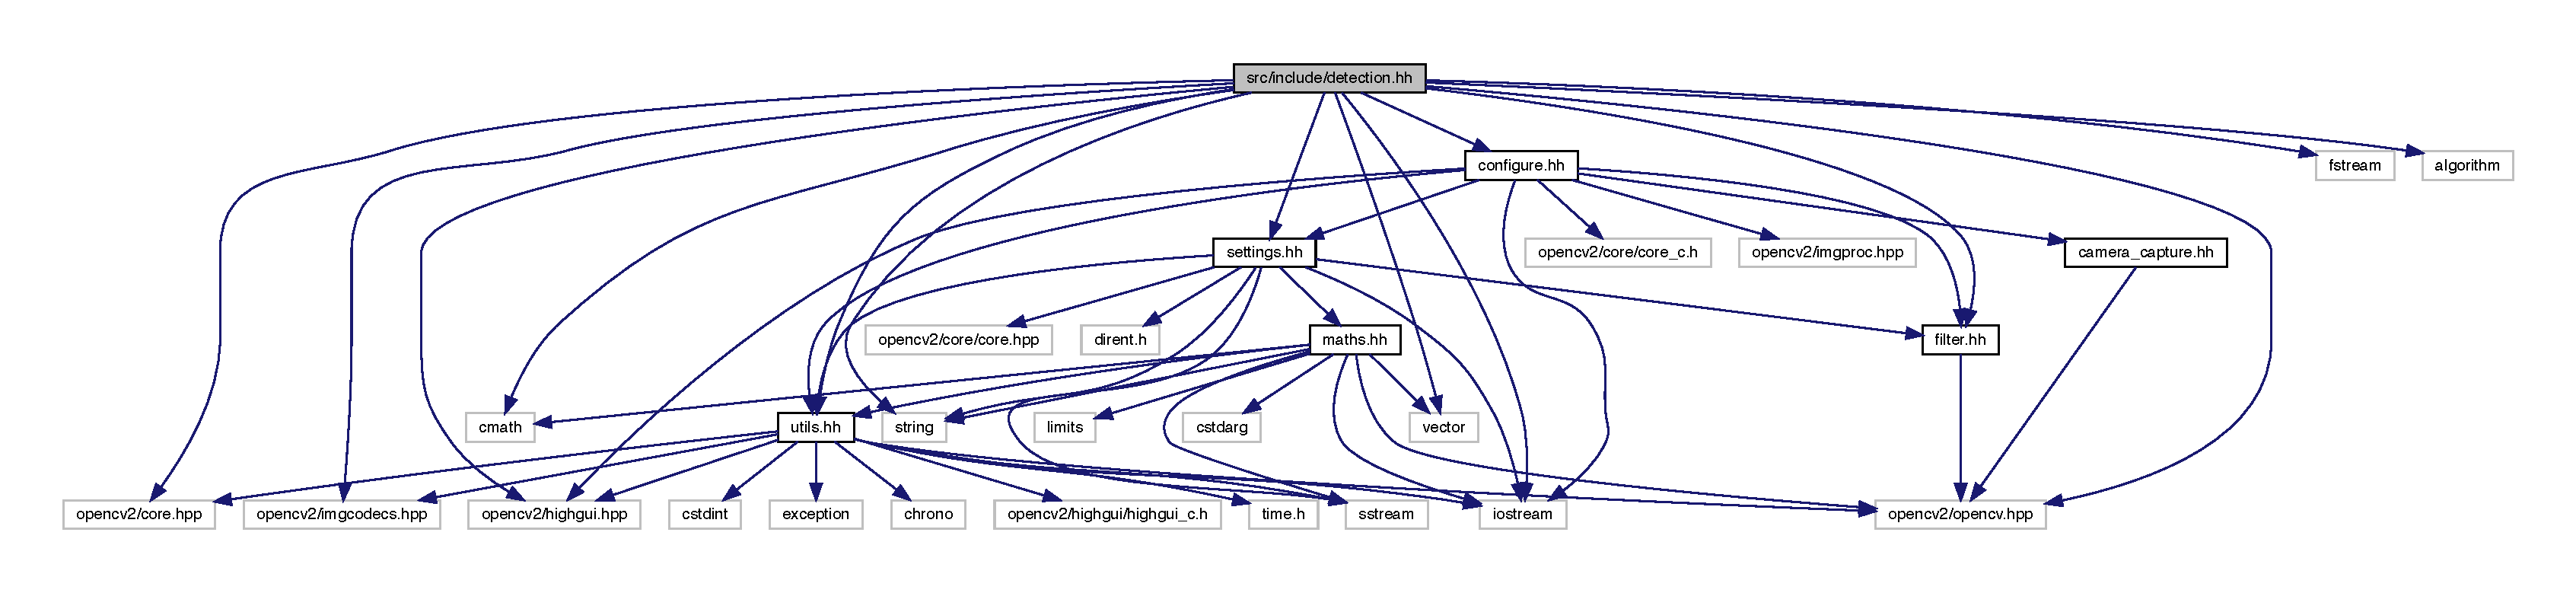
\includegraphics[width=350pt]{detection_8hh__incl}
\end{center}
\end{figure}
This graph shows which files directly or indirectly include this file\+:
\nopagebreak
\begin{figure}[H]
\begin{center}
\leavevmode
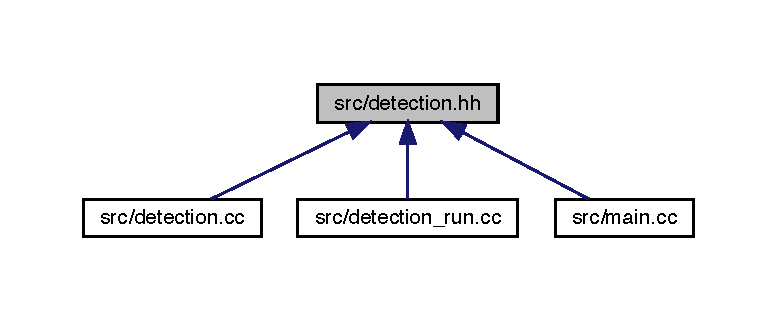
\includegraphics[width=350pt]{detection_8hh__dep__incl}
\end{center}
\end{figure}
\subsection*{Functions}
\begin{DoxyCompactItemize}
\item 
\mbox{\hyperlink{draw_8hh_aa620a13339ac3a1177c86edc549fda9b}{int}} \mbox{\hyperlink{detection_8hh_a17e13c447692201697b084a1906cf6fb}{detection}} ()
\begin{DoxyCompactList}\small\item\em Loads some images and detects shapes according to different colors. \end{DoxyCompactList}\item 
void \mbox{\hyperlink{detection_8hh_ac47563337453ac7d1314fe83218c87fc}{shape\+\_\+detection}} (const Mat \&img, const \mbox{\hyperlink{draw_8hh_aa620a13339ac3a1177c86edc549fda9b}{int}} color, const Mat \&un\+\_\+img)
\begin{DoxyCompactList}\small\item\em Detect shapes inside the image according to the variable \textquotesingle{}color\textquotesingle{}. \end{DoxyCompactList}\item 
void \mbox{\hyperlink{detection_8hh_a28d0cdb56cfb2164f939dc2f83d1d9d0}{erode\+\_\+dilation}} (Mat \&img, const \mbox{\hyperlink{draw_8hh_aa620a13339ac3a1177c86edc549fda9b}{int}} color)
\begin{DoxyCompactList}\small\item\em It apply some filtering function for isolate the subject and remove the noise. \end{DoxyCompactList}\item 
void \mbox{\hyperlink{detection_8hh_a93844a9ac3d8be0bd871bb41f8260330}{find\+\_\+contours}} (const Mat \&img, Mat original, const \mbox{\hyperlink{draw_8hh_aa620a13339ac3a1177c86edc549fda9b}{int}} color)
\begin{DoxyCompactList}\small\item\em Given an image, in black/white format, identify all the borders that delimit the shapes. \end{DoxyCompactList}\item 
\mbox{\hyperlink{draw_8hh_aa620a13339ac3a1177c86edc549fda9b}{int}} \mbox{\hyperlink{detection_8hh_a785fcf35ca81d113a1ea3d831fbdbc22}{number\+\_\+recognition}} (Rect blob, const Mat \&base)
\begin{DoxyCompactList}\small\item\em Detect a number on an image inside a region of interest. \end{DoxyCompactList}\item 
void \mbox{\hyperlink{detection_8hh_a923b178671e2272c6b082335d118716a}{save\+\_\+convex\+\_\+hull}} (const vector$<$ vector$<$ Point $>$$>$ \&contours, const \mbox{\hyperlink{draw_8hh_aa620a13339ac3a1177c86edc549fda9b}{int}} color, const vector$<$ \mbox{\hyperlink{draw_8hh_aa620a13339ac3a1177c86edc549fda9b}{int}} $>$ \&victims)
\begin{DoxyCompactList}\small\item\em Given some vector save it in a xml file. \end{DoxyCompactList}\item 
void \mbox{\hyperlink{detection_8hh_a50993b0aa4f01d89a4e5d0aef4e1e5f4}{load\+\_\+number\+\_\+template}} ()
\begin{DoxyCompactList}\small\item\em Load some templates and save them in the global variable \textquotesingle{}templates\textquotesingle{}. \end{DoxyCompactList}\item 
void \mbox{\hyperlink{detection_8hh_a8edaf0da54add7cd1461bafecef26b56}{crop\+\_\+number\+\_\+section}} (Mat \&process\+R\+OI)
\begin{DoxyCompactList}\small\item\em Given an image identify the region of interest(\+R\+O\+I) and crop it out. \end{DoxyCompactList}\end{DoxyCompactItemize}


\subsection{Function Documentation}
\mbox{\Hypertarget{detection_8hh_a8edaf0da54add7cd1461bafecef26b56}\label{detection_8hh_a8edaf0da54add7cd1461bafecef26b56}} 
\index{detection.hh@{detection.hh}!crop\_number\_section@{crop\_number\_section}}
\index{crop\_number\_section@{crop\_number\_section}!detection.hh@{detection.hh}}
\subsubsection{\texorpdfstring{crop\_number\_section()}{crop\_number\_section()}}
{\footnotesize\ttfamily void crop\+\_\+number\+\_\+section (\begin{DoxyParamCaption}\item[{Mat \&}]{R\+OI }\end{DoxyParamCaption})}



Given an image identify the region of interest(\+R\+O\+I) and crop it out. 


\begin{DoxyParams}[1]{Parameters}
\mbox{\texttt{ in,out}}  & {\em R\+OI} & Is the image that the function will going to elaborate. \\
\hline
\end{DoxyParams}
\mbox{\Hypertarget{detection_8hh_a17e13c447692201697b084a1906cf6fb}\label{detection_8hh_a17e13c447692201697b084a1906cf6fb}} 
\index{detection.hh@{detection.hh}!detection@{detection}}
\index{detection@{detection}!detection.hh@{detection.hh}}
\subsubsection{\texorpdfstring{detection()}{detection()}}
{\footnotesize\ttfamily \mbox{\hyperlink{draw_8hh_aa620a13339ac3a1177c86edc549fda9b}{int}} detection (\begin{DoxyParamCaption}{ }\end{DoxyParamCaption})}



Loads some images and detects shapes according to different colors. 

\begin{DoxyReturn}{Returns}
Return 0 if the function reach the end. 
\end{DoxyReturn}
\mbox{\Hypertarget{detection_8hh_a28d0cdb56cfb2164f939dc2f83d1d9d0}\label{detection_8hh_a28d0cdb56cfb2164f939dc2f83d1d9d0}} 
\index{detection.hh@{detection.hh}!erode\_dilation@{erode\_dilation}}
\index{erode\_dilation@{erode\_dilation}!detection.hh@{detection.hh}}
\subsubsection{\texorpdfstring{erode\_dilation()}{erode\_dilation()}}
{\footnotesize\ttfamily void erode\+\_\+dilation (\begin{DoxyParamCaption}\item[{Mat \&}]{img,  }\item[{const \mbox{\hyperlink{draw_8hh_aa620a13339ac3a1177c86edc549fda9b}{int}}}]{color }\end{DoxyParamCaption})}



It apply some filtering function for isolate the subject and remove the noise. 

An example of the sub functions called are\+: Gaussian\+Blur, Erosion, Dilation and Threshold.


\begin{DoxyParams}[1]{Parameters}
\mbox{\texttt{ in,out}}  & {\em img} & Is the image on which the function apply the filtering. \\
\hline
\mbox{\texttt{ in}}  & {\em color} & Can has 4 value\+:~\newline
0 -\/$>$ Red~\newline
1 -\/$>$ Green~\newline
2 -\/$>$ Blue~\newline
3 -\/$>$ Black~\newline
According to the color the filtering functions apply can change in the type and in the order. \\
\hline
\end{DoxyParams}
\mbox{\Hypertarget{detection_8hh_a93844a9ac3d8be0bd871bb41f8260330}\label{detection_8hh_a93844a9ac3d8be0bd871bb41f8260330}} 
\index{detection.hh@{detection.hh}!find\_contours@{find\_contours}}
\index{find\_contours@{find\_contours}!detection.hh@{detection.hh}}
\subsubsection{\texorpdfstring{find\_contours()}{find\_contours()}}
{\footnotesize\ttfamily void find\+\_\+contours (\begin{DoxyParamCaption}\item[{const Mat \&}]{img,  }\item[{Mat}]{original,  }\item[{const \mbox{\hyperlink{draw_8hh_aa620a13339ac3a1177c86edc549fda9b}{int}}}]{color }\end{DoxyParamCaption})}



Given an image, in black/white format, identify all the borders that delimit the shapes. 


\begin{DoxyParams}[1]{Parameters}
\mbox{\texttt{ in}}  & {\em img} & Is an image in H\+SV format at the base of the elaboration process. \\
\hline
\mbox{\texttt{ out}}  & {\em original} & Is the original source of \textquotesingle{}img\textquotesingle{}, it is used for showing the detected contours. \\
\hline
\mbox{\texttt{ in}}  & {\em color} & Can has 3 value\+:~\newline
0 -\/$>$ Red~\newline
1 -\/$>$ Green~\newline
2 -\/$>$ Blue~\newline
Is used for decid which procedure apply to the image. \\
\hline
\end{DoxyParams}
\mbox{\Hypertarget{detection_8hh_a50993b0aa4f01d89a4e5d0aef4e1e5f4}\label{detection_8hh_a50993b0aa4f01d89a4e5d0aef4e1e5f4}} 
\index{detection.hh@{detection.hh}!load\_number\_template@{load\_number\_template}}
\index{load\_number\_template@{load\_number\_template}!detection.hh@{detection.hh}}
\subsubsection{\texorpdfstring{load\_number\_template()}{load\_number\_template()}}
{\footnotesize\ttfamily void load\+\_\+number\+\_\+template (\begin{DoxyParamCaption}{ }\end{DoxyParamCaption})}



Load some templates and save them in the global variable \textquotesingle{}templates\textquotesingle{}. 

\mbox{\Hypertarget{detection_8hh_a785fcf35ca81d113a1ea3d831fbdbc22}\label{detection_8hh_a785fcf35ca81d113a1ea3d831fbdbc22}} 
\index{detection.hh@{detection.hh}!number\_recognition@{number\_recognition}}
\index{number\_recognition@{number\_recognition}!detection.hh@{detection.hh}}
\subsubsection{\texorpdfstring{number\_recognition()}{number\_recognition()}}
{\footnotesize\ttfamily \mbox{\hyperlink{draw_8hh_aa620a13339ac3a1177c86edc549fda9b}{int}} number\+\_\+recognition (\begin{DoxyParamCaption}\item[{Rect}]{blob,  }\item[{const Mat \&}]{base }\end{DoxyParamCaption})}



Detect a number on an image inside a region of interest. 


\begin{DoxyParams}[1]{Parameters}
\mbox{\texttt{ in}}  & {\em blob} & Identify the region of interest inside the image \textquotesingle{}base\textquotesingle{}. \\
\hline
\mbox{\texttt{ in}}  & {\em base} & Is the image where the function will going to search the number.\\
\hline
\end{DoxyParams}
\begin{DoxyReturn}{Returns}
The number recognise, \textquotesingle{}-\/1\textquotesingle{} otherwise. 
\end{DoxyReturn}
\mbox{\Hypertarget{detection_8hh_a923b178671e2272c6b082335d118716a}\label{detection_8hh_a923b178671e2272c6b082335d118716a}} 
\index{detection.hh@{detection.hh}!save\_convex\_hull@{save\_convex\_hull}}
\index{save\_convex\_hull@{save\_convex\_hull}!detection.hh@{detection.hh}}
\subsubsection{\texorpdfstring{save\_convex\_hull()}{save\_convex\_hull()}}
{\footnotesize\ttfamily void save\+\_\+convex\+\_\+hull (\begin{DoxyParamCaption}\item[{const vector$<$ vector$<$ Point $>$$>$ \&}]{contours,  }\item[{const \mbox{\hyperlink{draw_8hh_aa620a13339ac3a1177c86edc549fda9b}{int}}}]{color,  }\item[{const vector$<$ \mbox{\hyperlink{draw_8hh_aa620a13339ac3a1177c86edc549fda9b}{int}} $>$ \&}]{victims }\end{DoxyParamCaption})}



Given some vector save it in a xml file. 


\begin{DoxyParams}[1]{Parameters}
\mbox{\texttt{ in}}  & {\em contours} & Is a vector that is saved in a xml file. \\
\hline
\mbox{\texttt{ in}}  & {\em color} & Is the parameter according to which the function decide if saved (\textquotesingle{}color==1\textquotesingle{}) or not (\textquotesingle{}otherwise\textquotesingle{}) the vector \textquotesingle{}victims\textquotesingle{}. \\
\hline
\mbox{\texttt{ in}}  & {\em victims} & Is a vector that is saved in a xml file. \\
\hline
\end{DoxyParams}
\mbox{\Hypertarget{detection_8hh_ac47563337453ac7d1314fe83218c87fc}\label{detection_8hh_ac47563337453ac7d1314fe83218c87fc}} 
\index{detection.hh@{detection.hh}!shape\_detection@{shape\_detection}}
\index{shape\_detection@{shape\_detection}!detection.hh@{detection.hh}}
\subsubsection{\texorpdfstring{shape\_detection()}{shape\_detection()}}
{\footnotesize\ttfamily void shape\+\_\+detection (\begin{DoxyParamCaption}\item[{const Mat \&}]{img,  }\item[{const \mbox{\hyperlink{draw_8hh_aa620a13339ac3a1177c86edc549fda9b}{int}}}]{color,  }\item[{const Mat \&}]{un\+\_\+img }\end{DoxyParamCaption})}



Detect shapes inside the image according to the variable \textquotesingle{}color\textquotesingle{}. 


\begin{DoxyParams}[1]{Parameters}
\mbox{\texttt{ in}}  & {\em img} & Image on which the research will done. \\
\hline
\mbox{\texttt{ in}}  & {\em color} & Can has 3 value\+:~\newline
0 -\/$>$ Red~\newline
1 -\/$>$ Green~\newline
2 -\/$>$ Blue~\newline
These color identify the possible spectrum that the function search on the image. \\
\hline
\end{DoxyParams}

\hypertarget{detection__run_8cc}{}\section{src/run/detection\+\_\+run.cc File Reference}
\label{detection__run_8cc}\index{src/run/detection\_run.cc@{src/run/detection\_run.cc}}
{\ttfamily \#include $<$detection.\+hh$>$}\newline
Include dependency graph for detection\+\_\+run.\+cc\+:
\nopagebreak
\begin{figure}[H]
\begin{center}
\leavevmode
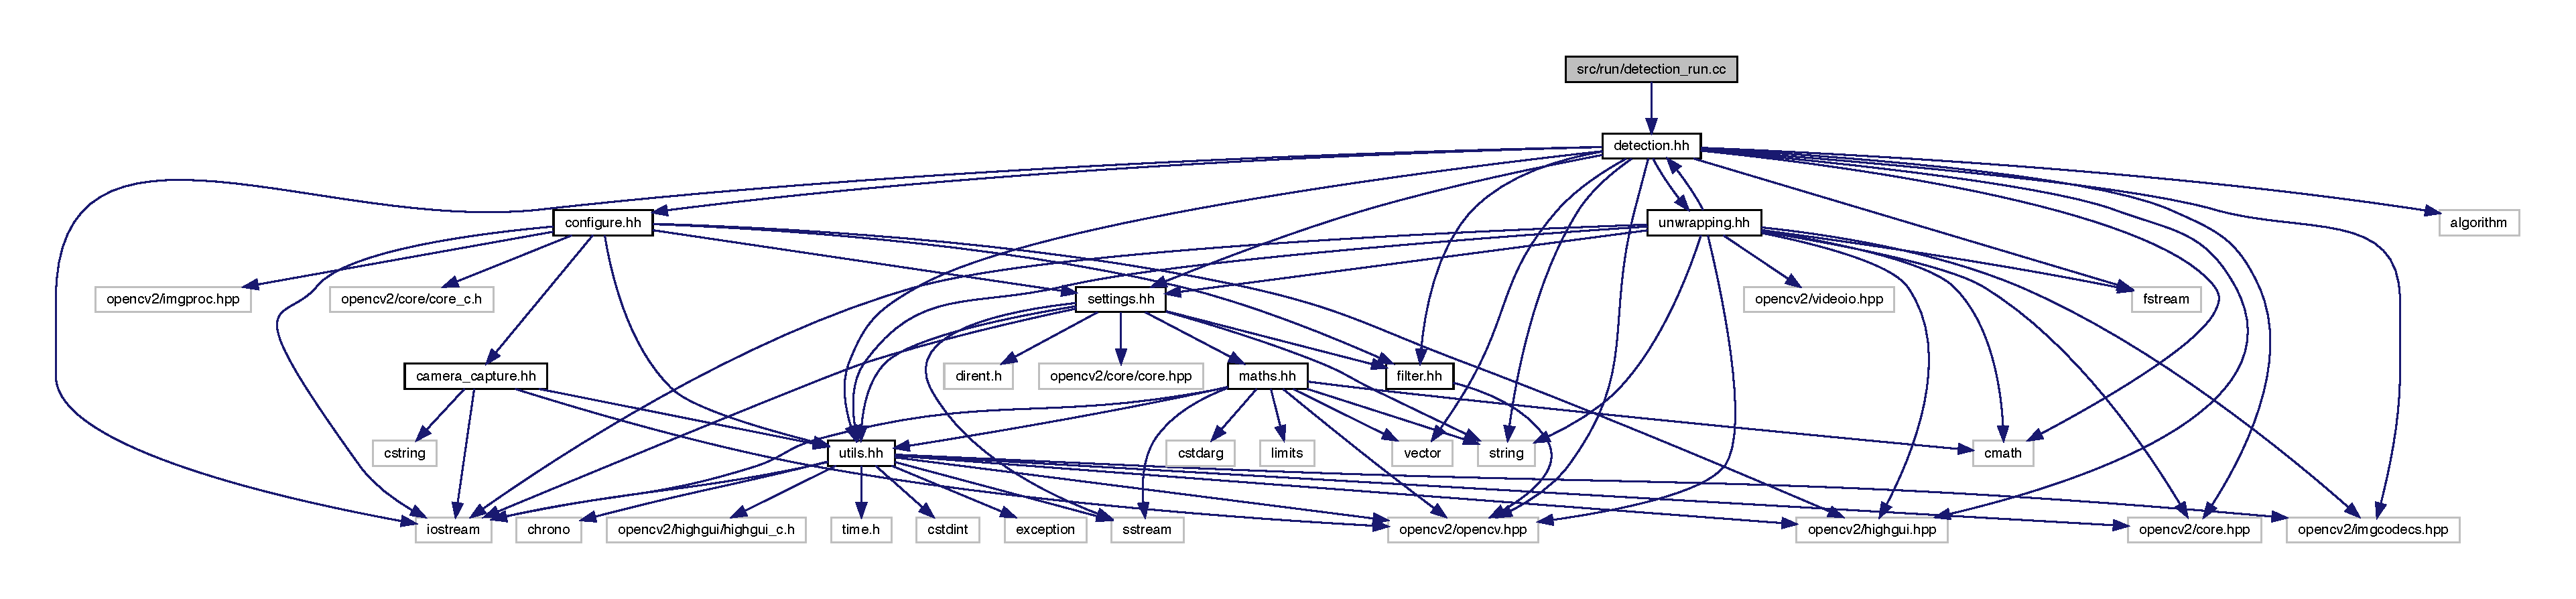
\includegraphics[width=350pt]{detection__run_8cc__incl}
\end{center}
\end{figure}
\subsection*{Functions}
\begin{DoxyCompactItemize}
\item 
\mbox{\hyperlink{draw_8hh_aa620a13339ac3a1177c86edc549fda9b}{int}} \mbox{\hyperlink{detection__run_8cc_ae66f6b31b5ad750f1fe042a706a4e3d4}{main}} ()
\end{DoxyCompactItemize}


\subsection{Function Documentation}
\mbox{\Hypertarget{detection__run_8cc_ae66f6b31b5ad750f1fe042a706a4e3d4}\label{detection__run_8cc_ae66f6b31b5ad750f1fe042a706a4e3d4}} 
\index{detection\_run.cc@{detection\_run.cc}!main@{main}}
\index{main@{main}!detection\_run.cc@{detection\_run.cc}}
\subsubsection{\texorpdfstring{main()}{main()}}
{\footnotesize\ttfamily \mbox{\hyperlink{draw_8hh_aa620a13339ac3a1177c86edc549fda9b}{int}} main (\begin{DoxyParamCaption}{ }\end{DoxyParamCaption})}


\hypertarget{dubins_8cc}{}\section{src/dubins.cc File Reference}
\label{dubins_8cc}\index{src/dubins.cc@{src/dubins.cc}}
{\ttfamily \#include \char`\"{}dubins.\+hh\char`\"{}}\newline
Include dependency graph for dubins.\+cc\+:
\nopagebreak
\begin{figure}[H]
\begin{center}
\leavevmode
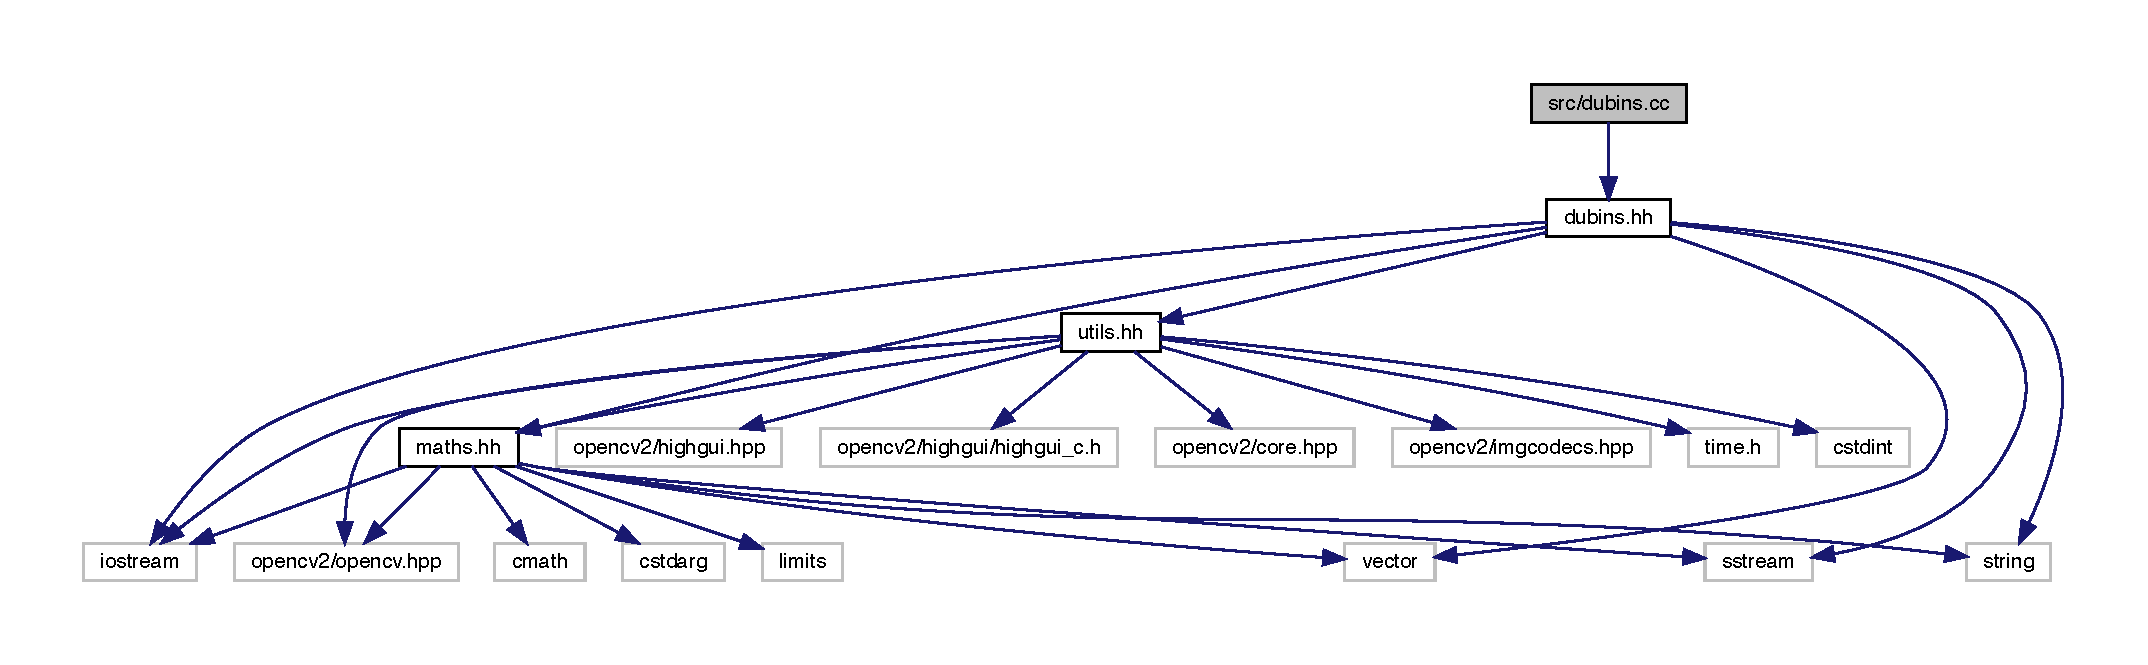
\includegraphics[width=350pt]{dubins_8cc__incl}
\end{center}
\end{figure}
\subsection*{Functions}
\begin{DoxyCompactItemize}
\item 
\mbox{\hyperlink{class_configuration2}{Configuration2}}$<$ double $>$ \mbox{\hyperlink{dubins_8cc_adef8b363044d7fed558e5b47d8d6a3a0}{circline}} (double \+\_\+L, \mbox{\hyperlink{class_configuration2}{Configuration2}}$<$ double $>$ \+\_\+\+P0, double \+\_\+K)
\item 
\mbox{\hyperlink{class_tuple}{Tuple}}$<$ \mbox{\hyperlink{class_angle}{Angle}} $>$ \mbox{\hyperlink{dubins_8cc_a24a357b93081a0180dfec16136bc8ff7}{to\+Base}} (\mbox{\hyperlink{class_tuple}{Tuple}}$<$ \mbox{\hyperlink{class_angle}{Angle}} $>$ z, \mbox{\hyperlink{draw_8hh_aa620a13339ac3a1177c86edc549fda9b}{int}} n, \mbox{\hyperlink{draw_8hh_aa620a13339ac3a1177c86edc549fda9b}{int}} base, const \mbox{\hyperlink{class_angle}{Angle}} \&inc, \mbox{\hyperlink{draw_8hh_aa620a13339ac3a1177c86edc549fda9b}{int}} start\+Pos, \mbox{\hyperlink{draw_8hh_aa620a13339ac3a1177c86edc549fda9b}{int}} end\+Pos)
\begin{DoxyCompactList}\small\item\em Convert a value in base 10 to base {\ttfamily base} in a {\ttfamily \mbox{\hyperlink{class_tuple}{Tuple}}}. To each value an inc is muiltiplied and the initial {\ttfamily \mbox{\hyperlink{class_angle}{Angle}}} is added. \end{DoxyCompactList}\item 
void \mbox{\hyperlink{dubins_8cc_ab93f9d42e66345d6252debb196f0f012}{disp}} (\mbox{\hyperlink{class_tuple}{Tuple}}$<$ \mbox{\hyperlink{class_tuple}{Tuple}}$<$ \mbox{\hyperlink{class_angle}{Angle}} $>$ $>$ \&t, \mbox{\hyperlink{class_tuple}{Tuple}}$<$ \mbox{\hyperlink{class_angle}{Angle}} $>$ \&z, \mbox{\hyperlink{draw_8hh_aa620a13339ac3a1177c86edc549fda9b}{int}} N, const \mbox{\hyperlink{class_angle}{Angle}} \&inc, \mbox{\hyperlink{draw_8hh_aa620a13339ac3a1177c86edc549fda9b}{int}} start\+Pos, \mbox{\hyperlink{draw_8hh_aa620a13339ac3a1177c86edc549fda9b}{int}} end\+Pos)
\begin{DoxyCompactList}\small\item\em Compute the arrangements. Since each arrangement can be computed as $n_{parts}$, where each values is then multiplied for the increment and is added to the initial values. \end{DoxyCompactList}\end{DoxyCompactItemize}


\subsection{Function Documentation}
\mbox{\Hypertarget{dubins_8cc_adef8b363044d7fed558e5b47d8d6a3a0}\label{dubins_8cc_adef8b363044d7fed558e5b47d8d6a3a0}} 
\index{dubins.cc@{dubins.cc}!circline@{circline}}
\index{circline@{circline}!dubins.cc@{dubins.cc}}
\subsubsection{\texorpdfstring{circline()}{circline()}}
{\footnotesize\ttfamily \mbox{\hyperlink{class_configuration2}{Configuration2}}$<$double$>$ circline (\begin{DoxyParamCaption}\item[{double}]{\+\_\+L,  }\item[{\mbox{\hyperlink{class_configuration2}{Configuration2}}$<$ double $>$}]{\+\_\+\+P0,  }\item[{double}]{\+\_\+K }\end{DoxyParamCaption})}

Computes an arrival point from an initial configuration through an arc of length \+\_\+L and curvature \+\_\+K. 
\begin{DoxyParams}[1]{Parameters}
\mbox{\texttt{ in}}  & {\em \+\_\+L} & The length of the arch. \\
\hline
\mbox{\texttt{ in}}  & {\em \+\_\+\+P0} & The starting {\ttfamily \mbox{\hyperlink{class_configuration2}{Configuration2}}} of the arc. \\
\hline
\mbox{\texttt{ in}}  & {\em \+\_\+K} & The curvature of the arc. \\
\hline
\end{DoxyParams}
\begin{DoxyReturn}{Returns}
The ending {\ttfamily \mbox{\hyperlink{class_configuration2}{Configuration2}}} of the arc. 
\end{DoxyReturn}
\mbox{\Hypertarget{dubins_8cc_ab93f9d42e66345d6252debb196f0f012}\label{dubins_8cc_ab93f9d42e66345d6252debb196f0f012}} 
\index{dubins.cc@{dubins.cc}!disp@{disp}}
\index{disp@{disp}!dubins.cc@{dubins.cc}}
\subsubsection{\texorpdfstring{disp()}{disp()}}
{\footnotesize\ttfamily void disp (\begin{DoxyParamCaption}\item[{\mbox{\hyperlink{class_tuple}{Tuple}}$<$ \mbox{\hyperlink{class_tuple}{Tuple}}$<$ \mbox{\hyperlink{class_angle}{Angle}} $>$ $>$ \&}]{t,  }\item[{\mbox{\hyperlink{class_tuple}{Tuple}}$<$ \mbox{\hyperlink{class_angle}{Angle}} $>$ \&}]{z,  }\item[{\mbox{\hyperlink{draw_8hh_aa620a13339ac3a1177c86edc549fda9b}{int}}}]{N,  }\item[{const \mbox{\hyperlink{class_angle}{Angle}} \&}]{inc,  }\item[{\mbox{\hyperlink{draw_8hh_aa620a13339ac3a1177c86edc549fda9b}{int}}}]{start\+Pos = {\ttfamily 0},  }\item[{\mbox{\hyperlink{draw_8hh_aa620a13339ac3a1177c86edc549fda9b}{int}}}]{end\+Pos = {\ttfamily 0} }\end{DoxyParamCaption})}



Compute the arrangements. Since each arrangement can be computed as $n_{parts}$, where each values is then multiplied for the increment and is added to the initial values. 


\begin{DoxyParams}[1]{Parameters}
\mbox{\texttt{ out}}  & {\em t} & A {\ttfamily \mbox{\hyperlink{class_tuple}{Tuple}}} containing all the {\ttfamily \mbox{\hyperlink{class_tuple}{Tuple}}}s containing the {\ttfamily \mbox{\hyperlink{class_angle}{Angle}}}s. \\
\hline
\mbox{\texttt{ in}}  & {\em z} & A {\ttfamily \mbox{\hyperlink{class_tuple}{Tuple}}} containing all the initial {\ttfamily \mbox{\hyperlink{class_angle}{Angle}}}s. \\
\hline
\mbox{\texttt{ in}}  & {\em N} & The number of iterations. Each iteration is going to be converted in base parts. \\
\hline
\mbox{\texttt{ in}}  & {\em inc} & The increment to give each initial {\ttfamily \mbox{\hyperlink{class_angle}{Angle}}}. \\
\hline
\mbox{\texttt{ in}}  & {\em start\+Pos} & The initial position to consider in {\ttfamily \mbox{\hyperlink{class_tuple}{Tuple}}}. \\
\hline
\mbox{\texttt{ in}}  & {\em end\+Pos} & The final position to consider in {\ttfamily \mbox{\hyperlink{class_tuple}{Tuple}}}. \\
\hline
\end{DoxyParams}
\mbox{\Hypertarget{dubins_8cc_a24a357b93081a0180dfec16136bc8ff7}\label{dubins_8cc_a24a357b93081a0180dfec16136bc8ff7}} 
\index{dubins.cc@{dubins.cc}!toBase@{toBase}}
\index{toBase@{toBase}!dubins.cc@{dubins.cc}}
\subsubsection{\texorpdfstring{toBase()}{toBase()}}
{\footnotesize\ttfamily \mbox{\hyperlink{class_tuple}{Tuple}}$<$\mbox{\hyperlink{class_angle}{Angle}}$>$ to\+Base (\begin{DoxyParamCaption}\item[{\mbox{\hyperlink{class_tuple}{Tuple}}$<$ \mbox{\hyperlink{class_angle}{Angle}} $>$}]{z,  }\item[{\mbox{\hyperlink{draw_8hh_aa620a13339ac3a1177c86edc549fda9b}{int}}}]{n,  }\item[{\mbox{\hyperlink{draw_8hh_aa620a13339ac3a1177c86edc549fda9b}{int}}}]{base,  }\item[{const \mbox{\hyperlink{class_angle}{Angle}} \&}]{inc,  }\item[{\mbox{\hyperlink{draw_8hh_aa620a13339ac3a1177c86edc549fda9b}{int}}}]{start\+Pos,  }\item[{\mbox{\hyperlink{draw_8hh_aa620a13339ac3a1177c86edc549fda9b}{int}}}]{end\+Pos }\end{DoxyParamCaption})}



Convert a value in base 10 to base {\ttfamily base} in a {\ttfamily \mbox{\hyperlink{class_tuple}{Tuple}}}. To each value an inc is muiltiplied and the initial {\ttfamily \mbox{\hyperlink{class_angle}{Angle}}} is added. 


\begin{DoxyParams}[1]{Parameters}
\mbox{\texttt{ in}}  & {\em z} & A {\ttfamily \mbox{\hyperlink{class_tuple}{Tuple}}} containing all the initial {\ttfamily \mbox{\hyperlink{class_angle}{Angle}}}s. \\
\hline
\mbox{\texttt{ in}}  & {\em n} & The value to be converted. \\
\hline
\mbox{\texttt{ in}}  & {\em base} & The base. \\
\hline
\mbox{\texttt{ in}}  & {\em inc} & The increment. \\
\hline
\mbox{\texttt{ in}}  & {\em start\+Pos} & The starting position of the {\ttfamily \mbox{\hyperlink{class_tuple}{Tuple}}} of {\ttfamily \mbox{\hyperlink{class_angle}{Angle}}}s. \\
\hline
\mbox{\texttt{ in}}  & {\em end\+Pos} & The ending position of the {\ttfamily \mbox{\hyperlink{class_tuple}{Tuple}}} of {\ttfamily \mbox{\hyperlink{class_angle}{Angle}}}s. \\
\hline
\end{DoxyParams}
\begin{DoxyReturn}{Returns}
A vector containing the digits of the number converted to the specified base. 
\end{DoxyReturn}

\hypertarget{dubins_8hh}{}\section{src/include/dubins.hh File Reference}
\label{dubins_8hh}\index{src/include/dubins.hh@{src/include/dubins.hh}}
{\ttfamily \#include $<$maths.\+hh$>$}\newline
{\ttfamily \#include $<$iostream$>$}\newline
{\ttfamily \#include $<$sstream$>$}\newline
{\ttfamily \#include $<$vector$>$}\newline
{\ttfamily \#include $<$string$>$}\newline
{\ttfamily \#include $<$utility$>$}\newline
Include dependency graph for dubins.\+hh\+:
\nopagebreak
\begin{figure}[H]
\begin{center}
\leavevmode
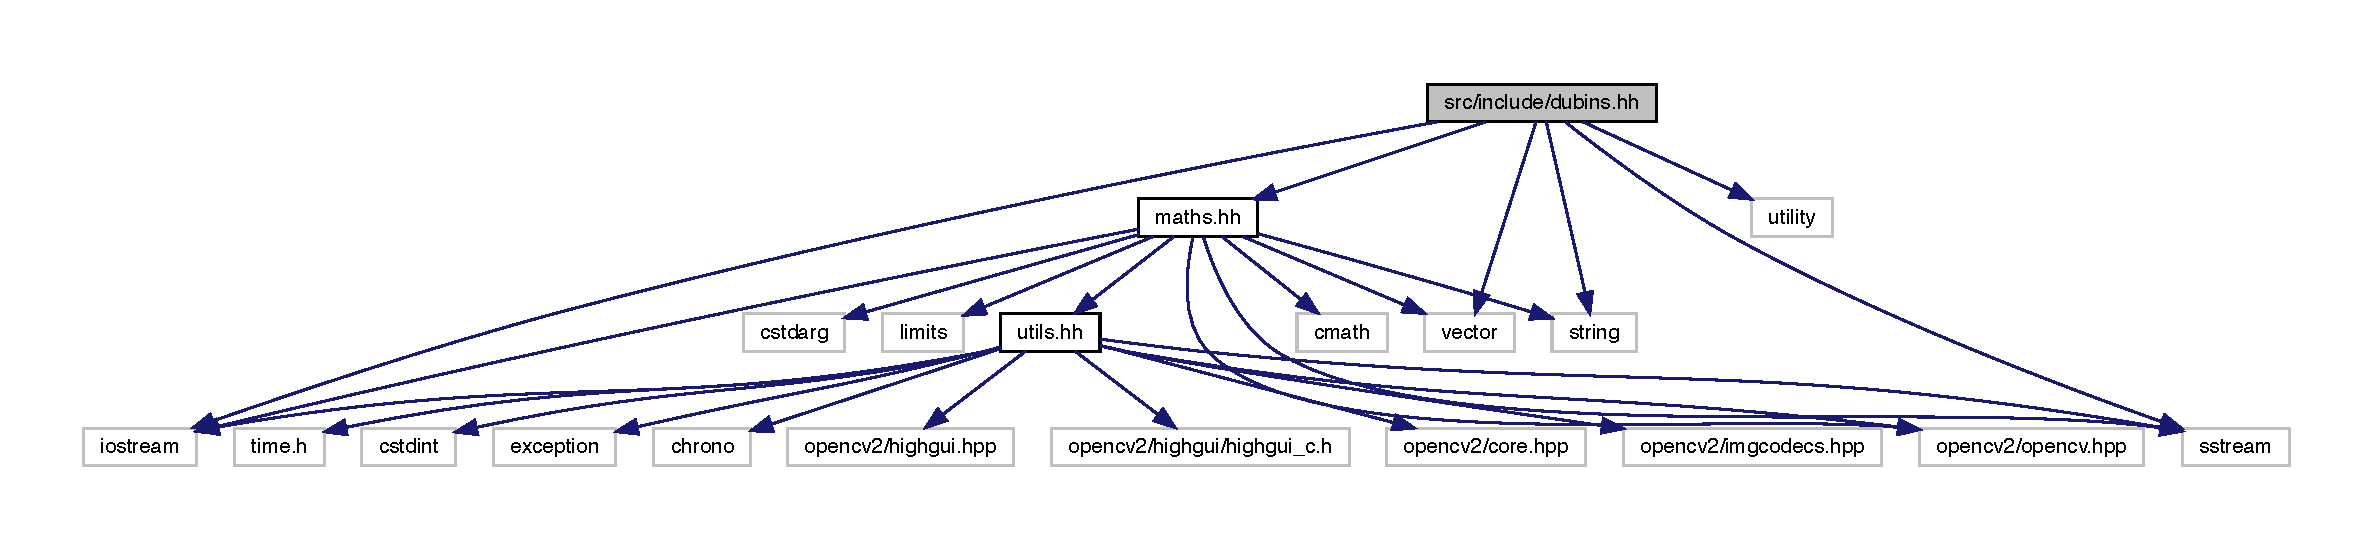
\includegraphics[width=350pt]{dubins_8hh__incl}
\end{center}
\end{figure}
This graph shows which files directly or indirectly include this file\+:
\nopagebreak
\begin{figure}[H]
\begin{center}
\leavevmode
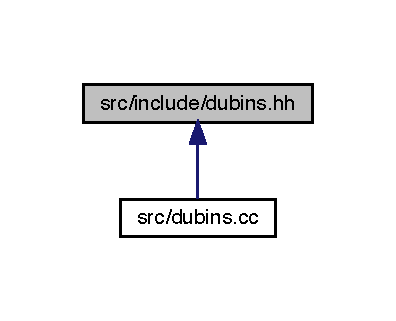
\includegraphics[width=190pt]{dubins_8hh__dep__incl}
\end{center}
\end{figure}
\subsection*{Classes}
\begin{DoxyCompactItemize}
\item 
class \mbox{\hyperlink{class_curve}{Curve$<$ T $>$}}
\item 
class \mbox{\hyperlink{class_dubins_arc}{Dubins\+Arc$<$ T1, T2 $>$}}
\begin{DoxyCompactList}\small\item\em Class to store a maneuver of \mbox{\hyperlink{class_dubins}{Dubins}}. It inherits from {\ttfamily \mbox{\hyperlink{class_curve}{Curve}}}. Since each \mbox{\hyperlink{class_dubins}{Dubins}} is formed of atmost 3 maneuvers, this class is meant to store one of this maneuver, which can be L, R or S respectively Left, Right, Straight. \end{DoxyCompactList}\item 
class \mbox{\hyperlink{class_dubins}{Dubins$<$ T $>$}}
\begin{DoxyCompactList}\small\item\em Class to store a \mbox{\hyperlink{class_dubins}{Dubins}} curve. This class inherits from {\ttfamily \mbox{\hyperlink{class_curve}{Curve}}} and is composed of three {\ttfamily \mbox{\hyperlink{class_dubins_arc}{Dubins\+Arc}}}. \end{DoxyCompactList}\item 
class \mbox{\hyperlink{class_dubins_set}{Dubins\+Set$<$ T $>$}}
\begin{DoxyCompactList}\small\item\em Given a set of point, compute the shortest set of \mbox{\hyperlink{class_dubins}{Dubins}} that allows to go from start to end through all points. \end{DoxyCompactList}\end{DoxyCompactItemize}
\subsection*{Macros}
\begin{DoxyCompactItemize}
\item 
\#define \mbox{\hyperlink{dubins_8hh_a5b2500ca93a5100f73dc442d3cfea7d4}{P\+I\+E\+C\+E\+\_\+\+L\+E\+N\+G\+TH}}~2
\item 
\#define \mbox{\hyperlink{dubins_8hh_a2bda1a81ce3474772a8a1f165e54516e}{P\+R\+EC}}~100000
\item 
\#define \mbox{\hyperlink{dubins_8hh_a940b85a83458e94519f2685b33ddd276}{K\+M\+AX}}~0.\+5
\end{DoxyCompactItemize}
\subsection*{Functions}
\begin{DoxyCompactItemize}
\item 
static double \mbox{\hyperlink{dubins_8hh_a5c88710b236a514392351a4d13d2e767}{sinc}} (double t)
\item 
\mbox{\hyperlink{class_configuration2}{Configuration2}}$<$ double $>$ \mbox{\hyperlink{dubins_8hh_adef8b363044d7fed558e5b47d8d6a3a0}{circline}} (double \+\_\+L, \mbox{\hyperlink{class_configuration2}{Configuration2}}$<$ double $>$ \+\_\+\+P0, double \+\_\+K)
\item 
\mbox{\hyperlink{class_tuple}{Tuple}}$<$ \mbox{\hyperlink{class_angle}{Angle}} $>$ \mbox{\hyperlink{dubins_8hh_a24a357b93081a0180dfec16136bc8ff7}{to\+Base}} (\mbox{\hyperlink{class_tuple}{Tuple}}$<$ \mbox{\hyperlink{class_angle}{Angle}} $>$ z, \mbox{\hyperlink{draw_8hh_aa620a13339ac3a1177c86edc549fda9b}{int}} n, \mbox{\hyperlink{draw_8hh_aa620a13339ac3a1177c86edc549fda9b}{int}} base, const \mbox{\hyperlink{class_angle}{Angle}} \&inc, \mbox{\hyperlink{draw_8hh_aa620a13339ac3a1177c86edc549fda9b}{int}} start\+Pos, \mbox{\hyperlink{draw_8hh_aa620a13339ac3a1177c86edc549fda9b}{int}} end\+Pos)
\begin{DoxyCompactList}\small\item\em Convert a value in base 10 to base {\ttfamily base} in a {\ttfamily \mbox{\hyperlink{class_tuple}{Tuple}}}. To each value an inc is muiltiplied and the initial {\ttfamily \mbox{\hyperlink{class_angle}{Angle}}} is added. \end{DoxyCompactList}\item 
void \mbox{\hyperlink{dubins_8hh_a16cf89e561eae9ea10a39e40432af238}{disp}} (\mbox{\hyperlink{class_tuple}{Tuple}}$<$ \mbox{\hyperlink{class_tuple}{Tuple}}$<$ \mbox{\hyperlink{class_angle}{Angle}} $>$ $>$ \&t, \mbox{\hyperlink{class_tuple}{Tuple}}$<$ \mbox{\hyperlink{class_angle}{Angle}} $>$ \&z, \mbox{\hyperlink{draw_8hh_aa620a13339ac3a1177c86edc549fda9b}{int}} N, const \mbox{\hyperlink{class_angle}{Angle}} \&inc, \mbox{\hyperlink{draw_8hh_aa620a13339ac3a1177c86edc549fda9b}{int}} start\+Pos=0, \mbox{\hyperlink{draw_8hh_aa620a13339ac3a1177c86edc549fda9b}{int}} end\+Pos=0)
\begin{DoxyCompactList}\small\item\em Compute the arrangements. Since each arrangement can be computed as $n_{parts}$, where each values is then multiplied for the increment and is added to the initial values. \end{DoxyCompactList}\item 
{\footnotesize template$<$class T $>$ }\\vector$<$ \mbox{\hyperlink{class_point2}{Point2}}$<$ T $>$ $>$ \mbox{\hyperlink{dubins_8hh_ae0b0aa229802950d33214a8a9e63ce5e}{plan\+\_\+best}} (vector$<$ \mbox{\hyperlink{class_point2}{Point2}}$<$ T $>$ $>$ v\+Points)
\end{DoxyCompactItemize}
\subsection*{Variables}
\begin{DoxyCompactItemize}
\item 
double \mbox{\hyperlink{dubins_8hh_a5880c4830bf2ab16bad216015448eacb}{elapsed\+Scale}}
\item 
double \mbox{\hyperlink{dubins_8hh_aa36733aa8c8ca5849070a465409dbe81}{elapsed\+Primitives}}
\item 
double \mbox{\hyperlink{dubins_8hh_a0031b22718178ccc76a4d8178e582b25}{elapsed\+Best}}
\item 
double \mbox{\hyperlink{dubins_8hh_a2ea7ce6fc7223d1e06dc71644336d66f}{elapsed\+Arcs}}
\item 
double \mbox{\hyperlink{dubins_8hh_a06fc38271c4ca7f7799fa903d94cae5a}{elapsed\+Check}}
\item 
unsigned long \mbox{\hyperlink{dubins_8hh_abcfdf634840cd6f14ae6d0762ecd1f95}{count\+Tries}}
\item 
double \mbox{\hyperlink{dubins_8hh_addc0762dc6f907d08093d87133317157}{elapsed\+Var}}
\item 
double \mbox{\hyperlink{dubins_8hh_ad0abfff7e943d5425fde32277365912b}{elapsed\+Circ}}
\item 
double \mbox{\hyperlink{dubins_8hh_abb6d93608c94bd3bd63217dc721ea2bf}{elapsed\+Set}}
\item 
double \mbox{\hyperlink{dubins_8hh_af7f52b98e604497e1df6126251edffcf}{elapsed\+L\+SL}}
\item 
double \mbox{\hyperlink{dubins_8hh_a5381897b84c903a717eda9680319f40a}{elapsed\+R\+SR}}
\item 
double \mbox{\hyperlink{dubins_8hh_ada1c98b34a456476f08c5cafbfe893ad}{elapsed\+L\+SR}}
\item 
double \mbox{\hyperlink{dubins_8hh_acb44475744bcbfbdf6609efd02c6c6fb}{elapsed\+R\+SL}}
\item 
double \mbox{\hyperlink{dubins_8hh_a3972b672793842e7de439255254d3085}{elapsed\+R\+LR}}
\item 
double \mbox{\hyperlink{dubins_8hh_a715f7de2f92786df84a14e5a013b94e9}{elapsed\+L\+RL}}
\end{DoxyCompactItemize}


\subsection{Macro Definition Documentation}
\mbox{\Hypertarget{dubins_8hh_a940b85a83458e94519f2685b33ddd276}\label{dubins_8hh_a940b85a83458e94519f2685b33ddd276}} 
\index{dubins.hh@{dubins.hh}!KMAX@{KMAX}}
\index{KMAX@{KMAX}!dubins.hh@{dubins.hh}}
\subsubsection{\texorpdfstring{KMAX}{KMAX}}
{\footnotesize\ttfamily \#define K\+M\+AX~0.\+5}

\mbox{\Hypertarget{dubins_8hh_a5b2500ca93a5100f73dc442d3cfea7d4}\label{dubins_8hh_a5b2500ca93a5100f73dc442d3cfea7d4}} 
\index{dubins.hh@{dubins.hh}!PIECE\_LENGTH@{PIECE\_LENGTH}}
\index{PIECE\_LENGTH@{PIECE\_LENGTH}!dubins.hh@{dubins.hh}}
\subsubsection{\texorpdfstring{PIECE\_LENGTH}{PIECE\_LENGTH}}
{\footnotesize\ttfamily \#define P\+I\+E\+C\+E\+\_\+\+L\+E\+N\+G\+TH~2}

\mbox{\Hypertarget{dubins_8hh_a2bda1a81ce3474772a8a1f165e54516e}\label{dubins_8hh_a2bda1a81ce3474772a8a1f165e54516e}} 
\index{dubins.hh@{dubins.hh}!PREC@{PREC}}
\index{PREC@{PREC}!dubins.hh@{dubins.hh}}
\subsubsection{\texorpdfstring{PREC}{PREC}}
{\footnotesize\ttfamily \#define P\+R\+EC~100000}



\subsection{Function Documentation}
\mbox{\Hypertarget{dubins_8hh_adef8b363044d7fed558e5b47d8d6a3a0}\label{dubins_8hh_adef8b363044d7fed558e5b47d8d6a3a0}} 
\index{dubins.hh@{dubins.hh}!circline@{circline}}
\index{circline@{circline}!dubins.hh@{dubins.hh}}
\subsubsection{\texorpdfstring{circline()}{circline()}}
{\footnotesize\ttfamily \mbox{\hyperlink{class_configuration2}{Configuration2}}$<$double$>$ circline (\begin{DoxyParamCaption}\item[{double}]{\+\_\+L,  }\item[{\mbox{\hyperlink{class_configuration2}{Configuration2}}$<$ double $>$}]{\+\_\+\+P0,  }\item[{double}]{\+\_\+K }\end{DoxyParamCaption})}

Computes an arrival point from an initial configuration through an arc of length \+\_\+L and curvature \+\_\+K. 
\begin{DoxyParams}[1]{Parameters}
\mbox{\texttt{ in}}  & {\em \+\_\+L} & The length of the arch. \\
\hline
\mbox{\texttt{ in}}  & {\em \+\_\+\+P0} & The starting {\ttfamily \mbox{\hyperlink{class_configuration2}{Configuration2}}} of the arc. \\
\hline
\mbox{\texttt{ in}}  & {\em \+\_\+K} & The curvature of the arc. \\
\hline
\end{DoxyParams}
\begin{DoxyReturn}{Returns}
The ending {\ttfamily \mbox{\hyperlink{class_configuration2}{Configuration2}}} of the arc. 
\end{DoxyReturn}
\mbox{\Hypertarget{dubins_8hh_a16cf89e561eae9ea10a39e40432af238}\label{dubins_8hh_a16cf89e561eae9ea10a39e40432af238}} 
\index{dubins.hh@{dubins.hh}!disp@{disp}}
\index{disp@{disp}!dubins.hh@{dubins.hh}}
\subsubsection{\texorpdfstring{disp()}{disp()}}
{\footnotesize\ttfamily void disp (\begin{DoxyParamCaption}\item[{\mbox{\hyperlink{class_tuple}{Tuple}}$<$ \mbox{\hyperlink{class_tuple}{Tuple}}$<$ \mbox{\hyperlink{class_angle}{Angle}} $>$ $>$ \&}]{t,  }\item[{\mbox{\hyperlink{class_tuple}{Tuple}}$<$ \mbox{\hyperlink{class_angle}{Angle}} $>$ \&}]{z,  }\item[{\mbox{\hyperlink{draw_8hh_aa620a13339ac3a1177c86edc549fda9b}{int}}}]{N,  }\item[{const \mbox{\hyperlink{class_angle}{Angle}} \&}]{inc,  }\item[{\mbox{\hyperlink{draw_8hh_aa620a13339ac3a1177c86edc549fda9b}{int}}}]{start\+Pos = {\ttfamily 0},  }\item[{\mbox{\hyperlink{draw_8hh_aa620a13339ac3a1177c86edc549fda9b}{int}}}]{end\+Pos = {\ttfamily 0} }\end{DoxyParamCaption})}



Compute the arrangements. Since each arrangement can be computed as $n_{parts}$, where each values is then multiplied for the increment and is added to the initial values. 


\begin{DoxyParams}[1]{Parameters}
\mbox{\texttt{ out}}  & {\em t} & A {\ttfamily \mbox{\hyperlink{class_tuple}{Tuple}}} containing all the {\ttfamily \mbox{\hyperlink{class_tuple}{Tuple}}}s containing the {\ttfamily \mbox{\hyperlink{class_angle}{Angle}}}s. \\
\hline
\mbox{\texttt{ in}}  & {\em z} & A {\ttfamily \mbox{\hyperlink{class_tuple}{Tuple}}} containing all the initial {\ttfamily \mbox{\hyperlink{class_angle}{Angle}}}s. \\
\hline
\mbox{\texttt{ in}}  & {\em N} & The number of iterations. Each iteration is going to be converted in base parts. \\
\hline
\mbox{\texttt{ in}}  & {\em inc} & The increment to give each initial {\ttfamily \mbox{\hyperlink{class_angle}{Angle}}}. \\
\hline
\mbox{\texttt{ in}}  & {\em start\+Pos} & The initial position to consider in {\ttfamily \mbox{\hyperlink{class_tuple}{Tuple}}}. \\
\hline
\mbox{\texttt{ in}}  & {\em end\+Pos} & The final position to consider in {\ttfamily \mbox{\hyperlink{class_tuple}{Tuple}}}. \\
\hline
\end{DoxyParams}
\mbox{\Hypertarget{dubins_8hh_ae0b0aa229802950d33214a8a9e63ce5e}\label{dubins_8hh_ae0b0aa229802950d33214a8a9e63ce5e}} 
\index{dubins.hh@{dubins.hh}!plan\_best@{plan\_best}}
\index{plan\_best@{plan\_best}!dubins.hh@{dubins.hh}}
\subsubsection{\texorpdfstring{plan\_best()}{plan\_best()}}
{\footnotesize\ttfamily template$<$class T $>$ \\
vector$<$\mbox{\hyperlink{class_point2}{Point2}}$<$T$>$ $>$ plan\+\_\+best (\begin{DoxyParamCaption}\item[{vector$<$ \mbox{\hyperlink{class_point2}{Point2}}$<$ T $>$ $>$}]{v\+Points }\end{DoxyParamCaption})}

\mbox{\Hypertarget{dubins_8hh_a5c88710b236a514392351a4d13d2e767}\label{dubins_8hh_a5c88710b236a514392351a4d13d2e767}} 
\index{dubins.hh@{dubins.hh}!sinc@{sinc}}
\index{sinc@{sinc}!dubins.hh@{dubins.hh}}
\subsubsection{\texorpdfstring{sinc()}{sinc()}}
{\footnotesize\ttfamily static double sinc (\begin{DoxyParamCaption}\item[{double}]{t }\end{DoxyParamCaption})\hspace{0.3cm}{\ttfamily [static]}}

Compute the sinc of the function defined as\+: \[ sinc(t)=\frac{sin(t)}{t}\quad t\neq 0 1\quad t=0 \] 
\begin{DoxyParams}[1]{Parameters}
\mbox{\texttt{ in}}  & {\em t} & The value of the angle to be used. \\
\hline
\end{DoxyParams}
\begin{DoxyReturn}{Returns}
The result of the previous formula. 
\end{DoxyReturn}
\mbox{\Hypertarget{dubins_8hh_a24a357b93081a0180dfec16136bc8ff7}\label{dubins_8hh_a24a357b93081a0180dfec16136bc8ff7}} 
\index{dubins.hh@{dubins.hh}!toBase@{toBase}}
\index{toBase@{toBase}!dubins.hh@{dubins.hh}}
\subsubsection{\texorpdfstring{toBase()}{toBase()}}
{\footnotesize\ttfamily \mbox{\hyperlink{class_tuple}{Tuple}}$<$\mbox{\hyperlink{class_angle}{Angle}}$>$ to\+Base (\begin{DoxyParamCaption}\item[{\mbox{\hyperlink{class_tuple}{Tuple}}$<$ \mbox{\hyperlink{class_angle}{Angle}} $>$}]{z,  }\item[{\mbox{\hyperlink{draw_8hh_aa620a13339ac3a1177c86edc549fda9b}{int}}}]{n,  }\item[{\mbox{\hyperlink{draw_8hh_aa620a13339ac3a1177c86edc549fda9b}{int}}}]{base,  }\item[{const \mbox{\hyperlink{class_angle}{Angle}} \&}]{inc,  }\item[{\mbox{\hyperlink{draw_8hh_aa620a13339ac3a1177c86edc549fda9b}{int}}}]{start\+Pos,  }\item[{\mbox{\hyperlink{draw_8hh_aa620a13339ac3a1177c86edc549fda9b}{int}}}]{end\+Pos }\end{DoxyParamCaption})}



Convert a value in base 10 to base {\ttfamily base} in a {\ttfamily \mbox{\hyperlink{class_tuple}{Tuple}}}. To each value an inc is muiltiplied and the initial {\ttfamily \mbox{\hyperlink{class_angle}{Angle}}} is added. 


\begin{DoxyParams}[1]{Parameters}
\mbox{\texttt{ in}}  & {\em z} & A {\ttfamily \mbox{\hyperlink{class_tuple}{Tuple}}} containing all the initial {\ttfamily \mbox{\hyperlink{class_angle}{Angle}}}s. \\
\hline
\mbox{\texttt{ in}}  & {\em n} & The value to be converted. \\
\hline
\mbox{\texttt{ in}}  & {\em base} & The base. \\
\hline
\mbox{\texttt{ in}}  & {\em inc} & The increment. \\
\hline
\mbox{\texttt{ in}}  & {\em start\+Pos} & The starting position of the {\ttfamily \mbox{\hyperlink{class_tuple}{Tuple}}} of {\ttfamily \mbox{\hyperlink{class_angle}{Angle}}}s. \\
\hline
\mbox{\texttt{ in}}  & {\em end\+Pos} & The ending position of the {\ttfamily \mbox{\hyperlink{class_tuple}{Tuple}}} of {\ttfamily \mbox{\hyperlink{class_angle}{Angle}}}s. \\
\hline
\end{DoxyParams}
\begin{DoxyReturn}{Returns}
A vector containing the digits of the number converted to the specified base. 
\end{DoxyReturn}


\subsection{Variable Documentation}
\mbox{\Hypertarget{dubins_8hh_abcfdf634840cd6f14ae6d0762ecd1f95}\label{dubins_8hh_abcfdf634840cd6f14ae6d0762ecd1f95}} 
\index{dubins.hh@{dubins.hh}!countTries@{countTries}}
\index{countTries@{countTries}!dubins.hh@{dubins.hh}}
\subsubsection{\texorpdfstring{countTries}{countTries}}
{\footnotesize\ttfamily unsigned long count\+Tries}

\mbox{\Hypertarget{dubins_8hh_a2ea7ce6fc7223d1e06dc71644336d66f}\label{dubins_8hh_a2ea7ce6fc7223d1e06dc71644336d66f}} 
\index{dubins.hh@{dubins.hh}!elapsedArcs@{elapsedArcs}}
\index{elapsedArcs@{elapsedArcs}!dubins.hh@{dubins.hh}}
\subsubsection{\texorpdfstring{elapsedArcs}{elapsedArcs}}
{\footnotesize\ttfamily double elapsed\+Arcs}

\mbox{\Hypertarget{dubins_8hh_a0031b22718178ccc76a4d8178e582b25}\label{dubins_8hh_a0031b22718178ccc76a4d8178e582b25}} 
\index{dubins.hh@{dubins.hh}!elapsedBest@{elapsedBest}}
\index{elapsedBest@{elapsedBest}!dubins.hh@{dubins.hh}}
\subsubsection{\texorpdfstring{elapsedBest}{elapsedBest}}
{\footnotesize\ttfamily double elapsed\+Best}

\mbox{\Hypertarget{dubins_8hh_a06fc38271c4ca7f7799fa903d94cae5a}\label{dubins_8hh_a06fc38271c4ca7f7799fa903d94cae5a}} 
\index{dubins.hh@{dubins.hh}!elapsedCheck@{elapsedCheck}}
\index{elapsedCheck@{elapsedCheck}!dubins.hh@{dubins.hh}}
\subsubsection{\texorpdfstring{elapsedCheck}{elapsedCheck}}
{\footnotesize\ttfamily double elapsed\+Check}

\mbox{\Hypertarget{dubins_8hh_ad0abfff7e943d5425fde32277365912b}\label{dubins_8hh_ad0abfff7e943d5425fde32277365912b}} 
\index{dubins.hh@{dubins.hh}!elapsedCirc@{elapsedCirc}}
\index{elapsedCirc@{elapsedCirc}!dubins.hh@{dubins.hh}}
\subsubsection{\texorpdfstring{elapsedCirc}{elapsedCirc}}
{\footnotesize\ttfamily double elapsed\+Circ}

\mbox{\Hypertarget{dubins_8hh_a715f7de2f92786df84a14e5a013b94e9}\label{dubins_8hh_a715f7de2f92786df84a14e5a013b94e9}} 
\index{dubins.hh@{dubins.hh}!elapsedLRL@{elapsedLRL}}
\index{elapsedLRL@{elapsedLRL}!dubins.hh@{dubins.hh}}
\subsubsection{\texorpdfstring{elapsedLRL}{elapsedLRL}}
{\footnotesize\ttfamily double elapsed\+L\+RL}

\mbox{\Hypertarget{dubins_8hh_af7f52b98e604497e1df6126251edffcf}\label{dubins_8hh_af7f52b98e604497e1df6126251edffcf}} 
\index{dubins.hh@{dubins.hh}!elapsedLSL@{elapsedLSL}}
\index{elapsedLSL@{elapsedLSL}!dubins.hh@{dubins.hh}}
\subsubsection{\texorpdfstring{elapsedLSL}{elapsedLSL}}
{\footnotesize\ttfamily double elapsed\+L\+SL}

\mbox{\Hypertarget{dubins_8hh_ada1c98b34a456476f08c5cafbfe893ad}\label{dubins_8hh_ada1c98b34a456476f08c5cafbfe893ad}} 
\index{dubins.hh@{dubins.hh}!elapsedLSR@{elapsedLSR}}
\index{elapsedLSR@{elapsedLSR}!dubins.hh@{dubins.hh}}
\subsubsection{\texorpdfstring{elapsedLSR}{elapsedLSR}}
{\footnotesize\ttfamily double elapsed\+L\+SR}

\mbox{\Hypertarget{dubins_8hh_aa36733aa8c8ca5849070a465409dbe81}\label{dubins_8hh_aa36733aa8c8ca5849070a465409dbe81}} 
\index{dubins.hh@{dubins.hh}!elapsedPrimitives@{elapsedPrimitives}}
\index{elapsedPrimitives@{elapsedPrimitives}!dubins.hh@{dubins.hh}}
\subsubsection{\texorpdfstring{elapsedPrimitives}{elapsedPrimitives}}
{\footnotesize\ttfamily double elapsed\+Primitives}

\mbox{\Hypertarget{dubins_8hh_a3972b672793842e7de439255254d3085}\label{dubins_8hh_a3972b672793842e7de439255254d3085}} 
\index{dubins.hh@{dubins.hh}!elapsedRLR@{elapsedRLR}}
\index{elapsedRLR@{elapsedRLR}!dubins.hh@{dubins.hh}}
\subsubsection{\texorpdfstring{elapsedRLR}{elapsedRLR}}
{\footnotesize\ttfamily double elapsed\+R\+LR}

\mbox{\Hypertarget{dubins_8hh_acb44475744bcbfbdf6609efd02c6c6fb}\label{dubins_8hh_acb44475744bcbfbdf6609efd02c6c6fb}} 
\index{dubins.hh@{dubins.hh}!elapsedRSL@{elapsedRSL}}
\index{elapsedRSL@{elapsedRSL}!dubins.hh@{dubins.hh}}
\subsubsection{\texorpdfstring{elapsedRSL}{elapsedRSL}}
{\footnotesize\ttfamily double elapsed\+R\+SL}

\mbox{\Hypertarget{dubins_8hh_a5381897b84c903a717eda9680319f40a}\label{dubins_8hh_a5381897b84c903a717eda9680319f40a}} 
\index{dubins.hh@{dubins.hh}!elapsedRSR@{elapsedRSR}}
\index{elapsedRSR@{elapsedRSR}!dubins.hh@{dubins.hh}}
\subsubsection{\texorpdfstring{elapsedRSR}{elapsedRSR}}
{\footnotesize\ttfamily double elapsed\+R\+SR}

\mbox{\Hypertarget{dubins_8hh_a5880c4830bf2ab16bad216015448eacb}\label{dubins_8hh_a5880c4830bf2ab16bad216015448eacb}} 
\index{dubins.hh@{dubins.hh}!elapsedScale@{elapsedScale}}
\index{elapsedScale@{elapsedScale}!dubins.hh@{dubins.hh}}
\subsubsection{\texorpdfstring{elapsedScale}{elapsedScale}}
{\footnotesize\ttfamily double elapsed\+Scale}

\mbox{\Hypertarget{dubins_8hh_abb6d93608c94bd3bd63217dc721ea2bf}\label{dubins_8hh_abb6d93608c94bd3bd63217dc721ea2bf}} 
\index{dubins.hh@{dubins.hh}!elapsedSet@{elapsedSet}}
\index{elapsedSet@{elapsedSet}!dubins.hh@{dubins.hh}}
\subsubsection{\texorpdfstring{elapsedSet}{elapsedSet}}
{\footnotesize\ttfamily double elapsed\+Set}

\mbox{\Hypertarget{dubins_8hh_addc0762dc6f907d08093d87133317157}\label{dubins_8hh_addc0762dc6f907d08093d87133317157}} 
\index{dubins.hh@{dubins.hh}!elapsedVar@{elapsedVar}}
\index{elapsedVar@{elapsedVar}!dubins.hh@{dubins.hh}}
\subsubsection{\texorpdfstring{elapsedVar}{elapsedVar}}
{\footnotesize\ttfamily double elapsed\+Var}


\hypertarget{main_8cc}{}\section{src/run/main.cc File Reference}
\label{main_8cc}\index{src/run/main.cc@{src/run/main.cc}}
{\ttfamily \#include $<$detection.\+hh$>$}\newline
{\ttfamily \#include $<$unwrapping.\+hh$>$}\newline
{\ttfamily \#include $<$configure.\+hh$>$}\newline
{\ttfamily \#include $<$iostream$>$}\newline
Include dependency graph for main.\+cc\+:
\nopagebreak
\begin{figure}[H]
\begin{center}
\leavevmode
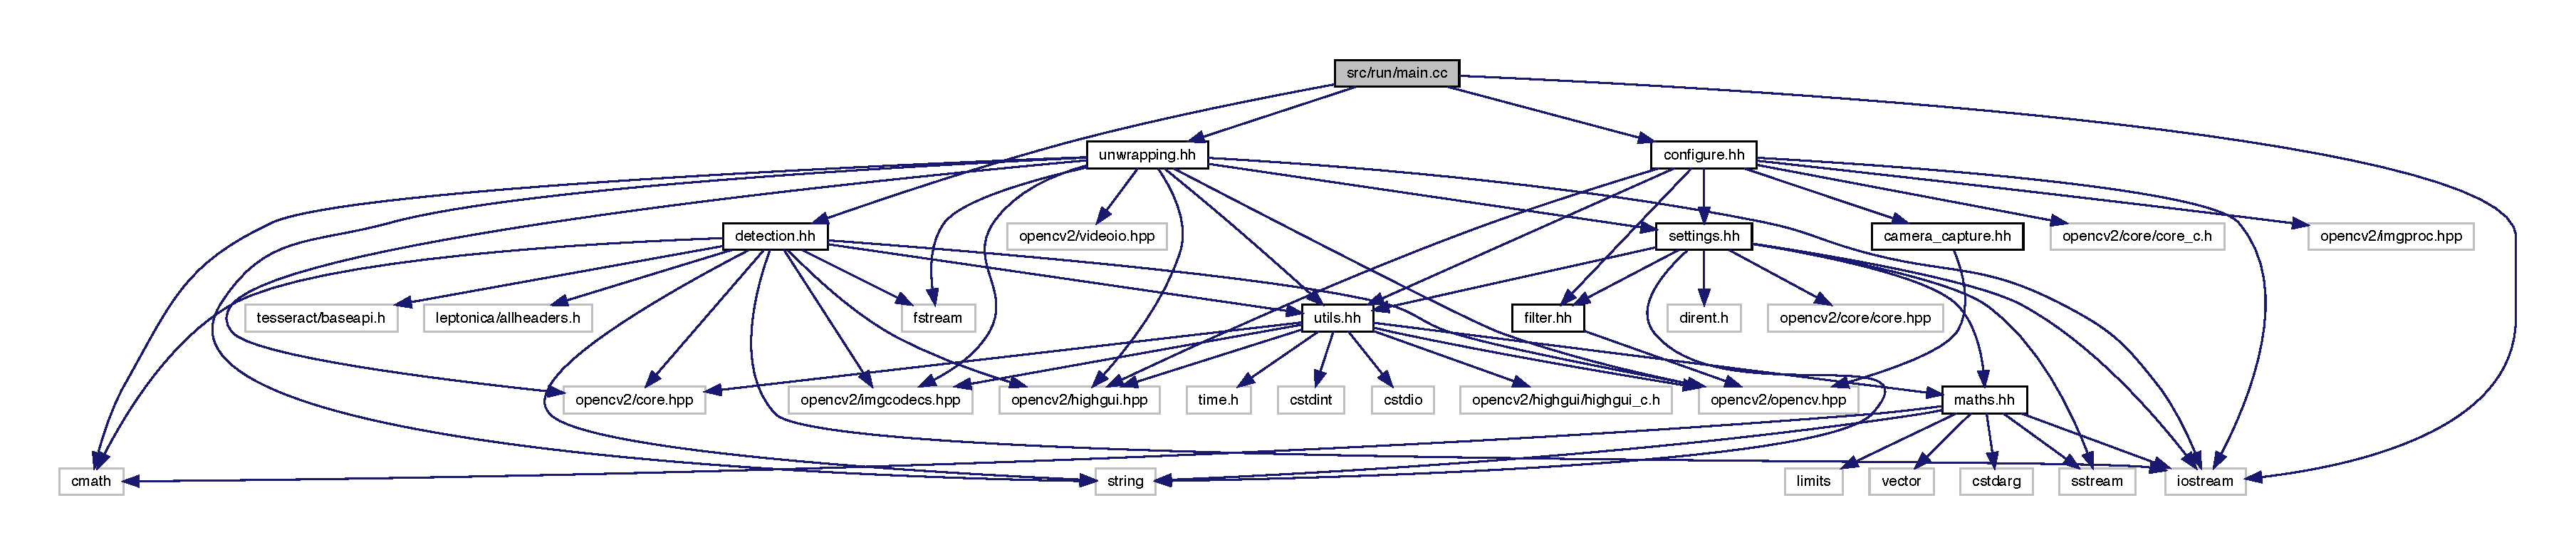
\includegraphics[width=350pt]{main_8cc__incl}
\end{center}
\end{figure}
\subsection*{Functions}
\begin{DoxyCompactItemize}
\item 
\mbox{\hyperlink{draw_8hh_aa620a13339ac3a1177c86edc549fda9b}{int}} \mbox{\hyperlink{main_8cc_ae66f6b31b5ad750f1fe042a706a4e3d4}{main}} ()
\end{DoxyCompactItemize}


\subsection{Function Documentation}
\mbox{\Hypertarget{main_8cc_ae66f6b31b5ad750f1fe042a706a4e3d4}\label{main_8cc_ae66f6b31b5ad750f1fe042a706a4e3d4}} 
\index{main.cc@{main.cc}!main@{main}}
\index{main@{main}!main.cc@{main.cc}}
\subsubsection{\texorpdfstring{main()}{main()}}
{\footnotesize\ttfamily \mbox{\hyperlink{draw_8hh_aa620a13339ac3a1177c86edc549fda9b}{int}} main (\begin{DoxyParamCaption}{ }\end{DoxyParamCaption})}


\hypertarget{maths_8cc}{}\section{src/maths.cc File Reference}
\label{maths_8cc}\index{src/maths.cc@{src/maths.cc}}
{\ttfamily \#include \char`\"{}maths.\+hh\char`\"{}}\newline
Include dependency graph for maths.\+cc\+:
\nopagebreak
\begin{figure}[H]
\begin{center}
\leavevmode
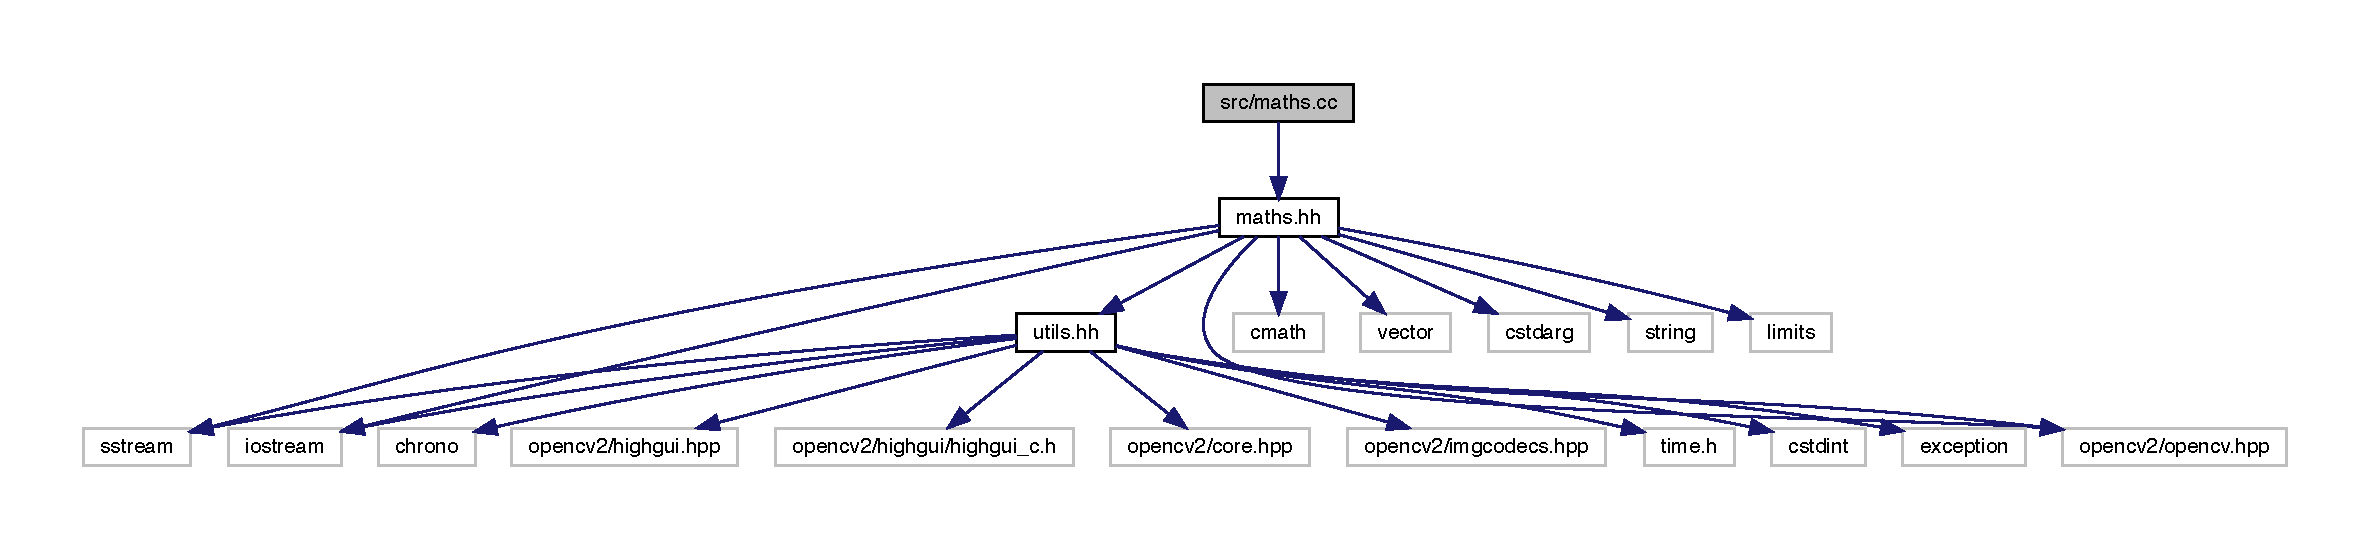
\includegraphics[width=350pt]{maths_8cc__incl}
\end{center}
\end{figure}
\subsection*{Functions}
\begin{DoxyCompactItemize}
\item 
void \mbox{\hyperlink{maths_8cc_a3af8b8654f1cdb8e8e4b8f72dcc5edd5}{invert\+Angle}} (\mbox{\hyperlink{class_angle}{Angle}} \&a)
\begin{DoxyCompactList}\small\item\em Transform the angle given i the new reference system where x and y will be swapped. \end{DoxyCompactList}\end{DoxyCompactItemize}


\subsection{Function Documentation}
\mbox{\Hypertarget{maths_8cc_a3af8b8654f1cdb8e8e4b8f72dcc5edd5}\label{maths_8cc_a3af8b8654f1cdb8e8e4b8f72dcc5edd5}} 
\index{maths.cc@{maths.cc}!invertAngle@{invertAngle}}
\index{invertAngle@{invertAngle}!maths.cc@{maths.cc}}
\subsubsection{\texorpdfstring{invertAngle()}{invertAngle()}}
{\footnotesize\ttfamily void invert\+Angle (\begin{DoxyParamCaption}\item[{\mbox{\hyperlink{class_angle}{Angle}} \&}]{a }\end{DoxyParamCaption})}



Transform the angle given i the new reference system where x and y will be swapped. 


\begin{DoxyParams}{Parameters}
{\em \mbox{[}in/out\mbox{]}} & a The angle that need to be inverted. \\
\hline
\end{DoxyParams}

\hypertarget{maths_8hh}{}\section{src/include/maths.hh File Reference}
\label{maths_8hh}\index{src/include/maths.hh@{src/include/maths.hh}}
{\ttfamily \#include $<$utils.\+hh$>$}\newline
{\ttfamily \#include $<$iostream$>$}\newline
{\ttfamily \#include $<$cmath$>$}\newline
{\ttfamily \#include $<$vector$>$}\newline
{\ttfamily \#include $<$cstdarg$>$}\newline
{\ttfamily \#include $<$sstream$>$}\newline
{\ttfamily \#include $<$string$>$}\newline
{\ttfamily \#include $<$opencv2/opencv.\+hpp$>$}\newline
{\ttfamily \#include $<$limits$>$}\newline
Include dependency graph for maths.\+hh\+:
\nopagebreak
\begin{figure}[H]
\begin{center}
\leavevmode
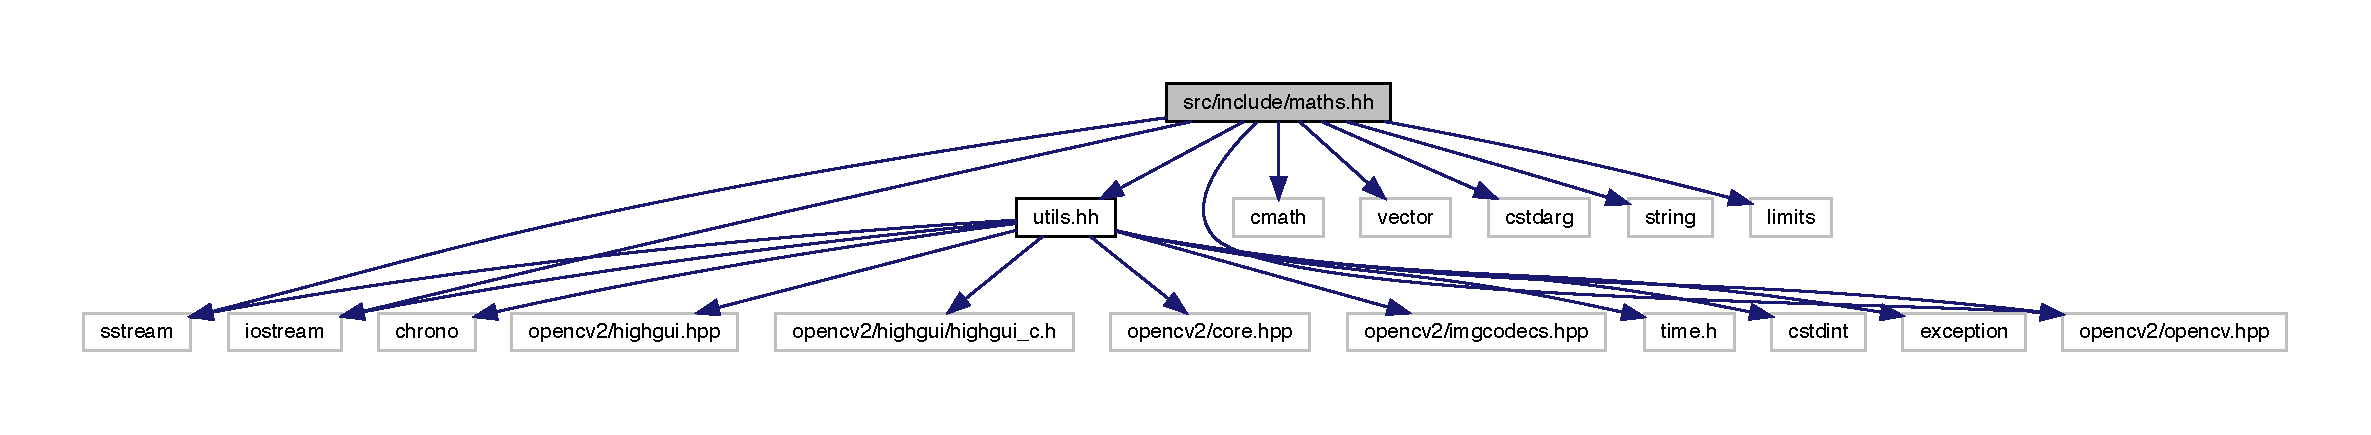
\includegraphics[width=350pt]{maths_8hh__incl}
\end{center}
\end{figure}
This graph shows which files directly or indirectly include this file\+:
\nopagebreak
\begin{figure}[H]
\begin{center}
\leavevmode
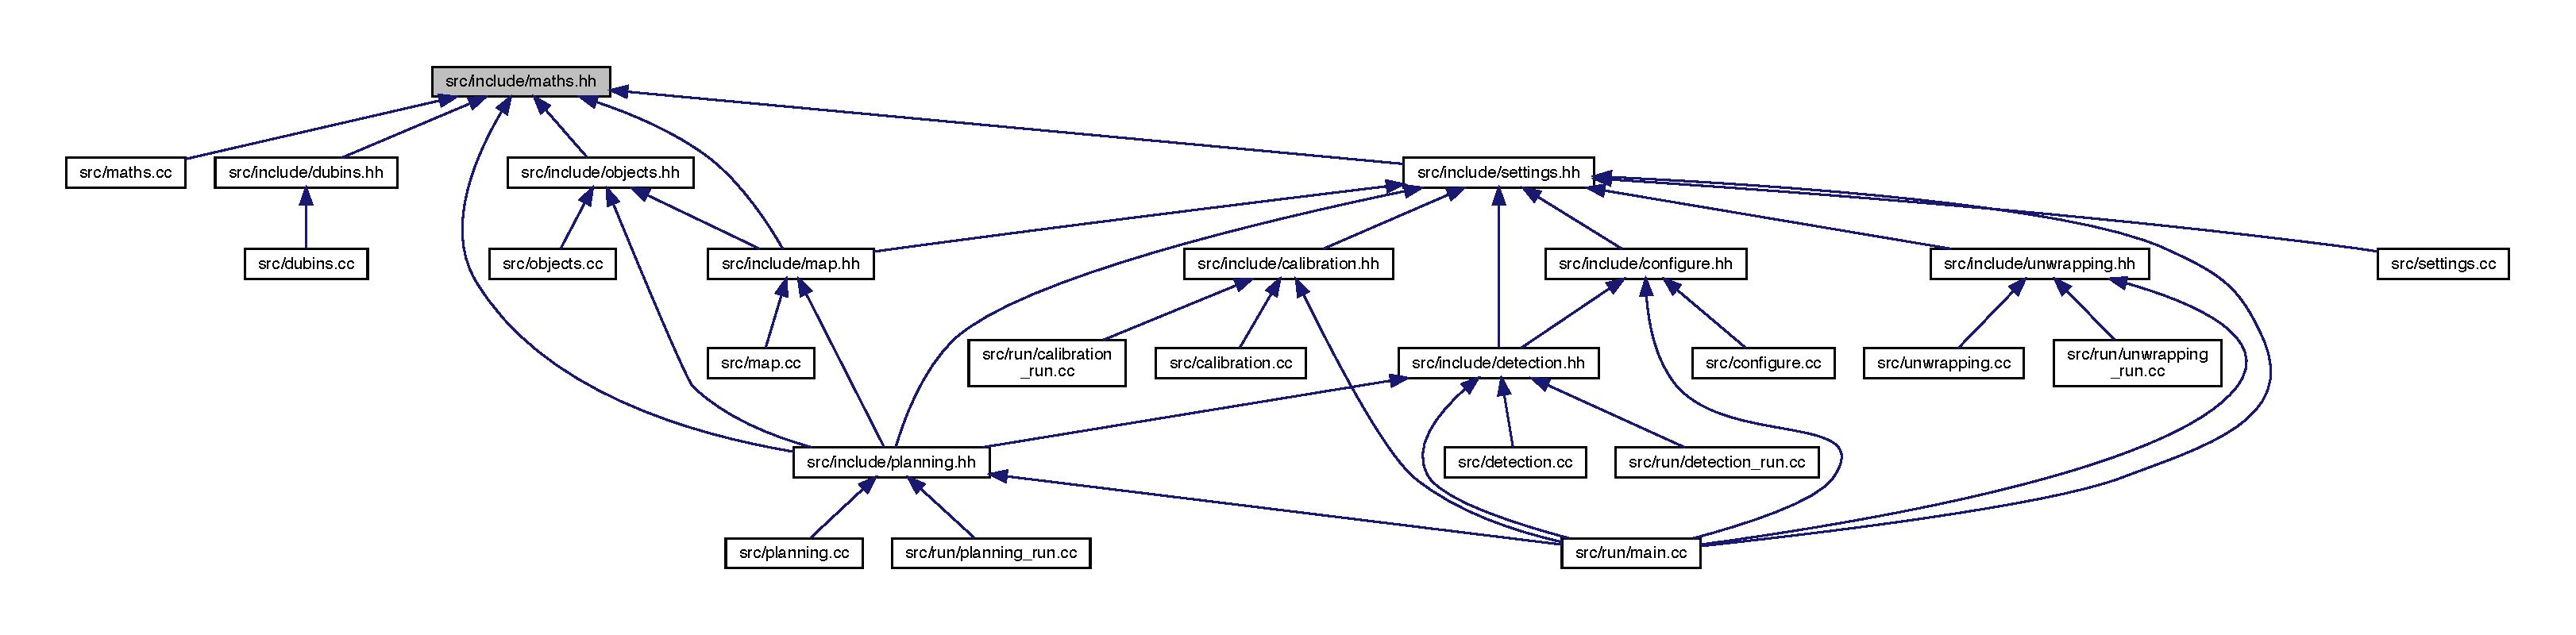
\includegraphics[width=350pt]{maths_8hh__dep__incl}
\end{center}
\end{figure}
\subsection*{Classes}
\begin{DoxyCompactItemize}
\item 
class \mbox{\hyperlink{class_angle}{Angle}}
\begin{DoxyCompactList}\small\item\em This class allows to save and handle angles. It supports D\+EG and R\+AD, operations such as addition and subtraction with operators overloading, conversion from R\+AD to D\+EG and viceversa and normalization of the angle. \end{DoxyCompactList}\item 
class \mbox{\hyperlink{class_tuple}{Tuple$<$ T $>$}}
\item 
class \mbox{\hyperlink{class_point2}{Point2$<$ T $>$}}
\begin{DoxyCompactList}\small\item\em Class that stores two value to construct a point in 2D. The value is saved in a \mbox{\hyperlink{class_tuple}{Tuple}}. \end{DoxyCompactList}\item 
class \mbox{\hyperlink{class_configuration2}{Configuration2$<$ T1 $>$}}
\begin{DoxyCompactList}\small\item\em This class stores a configuration, that is a point and an angle. \end{DoxyCompactList}\end{DoxyCompactItemize}
\subsection*{Macros}
\begin{DoxyCompactItemize}
\item 
\#define \mbox{\hyperlink{maths_8hh_a995779faef78614d4f074b7d444de767}{D\+Inf}}~numeric\+\_\+limits$<$double$>$\+::infinity()
\item 
\#define \mbox{\hyperlink{maths_8hh_a78802b279ab85021d7f6bffe51621703}{Epsi}}~numeric\+\_\+limits$<$double$>$\+::epsilon()
\item 
\#define \mbox{\hyperlink{maths_8hh_ad7760000c41920a1ae5cf0f6bf0e4c77}{A\+\_\+2\+PI}}~\mbox{\hyperlink{class_angle}{Angle}}(6.\+2831853071-\/\mbox{\hyperlink{maths_8hh_a78802b279ab85021d7f6bffe51621703}{Epsi}}, \mbox{\hyperlink{class_angle_a4f7b9849ce8780bcba95ca3ee45cff77a93ab6b68075fd7a6fe724fbde5b13c1f}{Angle\+::\+R\+AD}})
\begin{DoxyCompactList}\small\item\em Default \mbox{\hyperlink{class_angle}{Angle}} for 2pi rad. \end{DoxyCompactList}\item 
\#define \mbox{\hyperlink{maths_8hh_ae46eba4b5423f51b80f3446e128c6476}{A\+\_\+360}}~\mbox{\hyperlink{class_angle}{Angle}}(360.\+0-\/\mbox{\hyperlink{maths_8hh_a78802b279ab85021d7f6bffe51621703}{Epsi}}, \mbox{\hyperlink{class_angle_a4f7b9849ce8780bcba95ca3ee45cff77a65e2aa4bc05730c9c2e8fdaf73612282}{Angle\+::\+D\+EG}})
\begin{DoxyCompactList}\small\item\em Default \mbox{\hyperlink{class_angle}{Angle}} for 360 degree. \end{DoxyCompactList}\item 
\#define \mbox{\hyperlink{maths_8hh_ad37649758ce967343cee82772583fd9c}{A\+\_\+\+PI}}~\mbox{\hyperlink{class_angle}{Angle}}(M\+\_\+\+PI, \mbox{\hyperlink{class_angle_a4f7b9849ce8780bcba95ca3ee45cff77a93ab6b68075fd7a6fe724fbde5b13c1f}{Angle\+::\+R\+AD}})
\begin{DoxyCompactList}\small\item\em Default \mbox{\hyperlink{class_angle}{Angle}} for pi rad. \end{DoxyCompactList}\item 
\#define \mbox{\hyperlink{maths_8hh_ac37f3aecadc99641dd1c8b4c81d96f7e}{A\+\_\+180}}~\mbox{\hyperlink{class_angle}{Angle}}(180, \mbox{\hyperlink{class_angle_a4f7b9849ce8780bcba95ca3ee45cff77a65e2aa4bc05730c9c2e8fdaf73612282}{Angle\+::\+D\+EG}})
\begin{DoxyCompactList}\small\item\em Defualt \mbox{\hyperlink{class_angle}{Angle}} for 180 degree. \end{DoxyCompactList}\item 
\#define \mbox{\hyperlink{maths_8hh_a73d408ce54489e86b860679af5d24059}{A\+\_\+\+P\+I2}}~\mbox{\hyperlink{class_angle}{Angle}}(M\+\_\+\+PI/2.\+0, \mbox{\hyperlink{class_angle_a4f7b9849ce8780bcba95ca3ee45cff77a93ab6b68075fd7a6fe724fbde5b13c1f}{Angle\+::\+R\+AD}})
\begin{DoxyCompactList}\small\item\em Default \mbox{\hyperlink{class_angle}{Angle}} for pi/2 rad. \end{DoxyCompactList}\item 
\#define \mbox{\hyperlink{maths_8hh_ae49ec00d228075202319f793f89e39b5}{A\+\_\+90}}~\mbox{\hyperlink{class_angle}{Angle}}(90, \mbox{\hyperlink{class_angle_a4f7b9849ce8780bcba95ca3ee45cff77a65e2aa4bc05730c9c2e8fdaf73612282}{Angle\+::\+D\+EG}})
\begin{DoxyCompactList}\small\item\em Defualt \mbox{\hyperlink{class_angle}{Angle}} for 90 degree. \end{DoxyCompactList}\item 
\#define \mbox{\hyperlink{maths_8hh_abc6a1d62385f5e3f01509c97666fbbbb}{A\+\_\+\+D\+E\+G\+\_\+\+N\+U\+LL}}~\mbox{\hyperlink{class_angle}{Angle}}(0, \mbox{\hyperlink{class_angle_a4f7b9849ce8780bcba95ca3ee45cff77a65e2aa4bc05730c9c2e8fdaf73612282}{Angle\+::\+D\+EG}})
\begin{DoxyCompactList}\small\item\em Default \mbox{\hyperlink{class_angle}{Angle}} for 0 rad. \end{DoxyCompactList}\item 
\#define \mbox{\hyperlink{maths_8hh_a0da7d22251afe9ccf02289e0bceca28f}{A\+\_\+\+R\+A\+D\+\_\+\+N\+U\+LL}}~\mbox{\hyperlink{class_angle}{Angle}}(0, \mbox{\hyperlink{class_angle_a4f7b9849ce8780bcba95ca3ee45cff77a93ab6b68075fd7a6fe724fbde5b13c1f}{Angle\+::\+R\+AD}})
\begin{DoxyCompactList}\small\item\em Defualt \mbox{\hyperlink{class_angle}{Angle}} for 0 degree. \end{DoxyCompactList}\item 
\#define \mbox{\hyperlink{maths_8hh_ad22dcdeefda7d41523cc1604953eb6cc}{tuple\+Iter}}~typename vector$<$T$>$\+::iterator
\item 
\#define \mbox{\hyperlink{maths_8hh_a2eba794860251c1b30e532df32ee4d1b}{tuple\+Const\+Iter}}~const typename vector$<$T$>$\+::iterator
\end{DoxyCompactItemize}
\subsection*{Enumerations}
\begin{DoxyCompactItemize}
\item 
enum \mbox{\hyperlink{maths_8hh_ac50d7263b1cae8691420b86282b27f90}{D\+I\+S\+T\+A\+N\+C\+E\+\_\+\+T\+Y\+PE}} \{ \mbox{\hyperlink{maths_8hh_ac50d7263b1cae8691420b86282b27f90a81bbbc4428c3ff3f1327e94957e2b5f1}{E\+U\+C\+L\+I\+D\+E\+AN}}, 
\mbox{\hyperlink{maths_8hh_ac50d7263b1cae8691420b86282b27f90a9ae95b5995796e7e5f32fa482a5bff98}{M\+A\+N\+H\+A\+T\+T\+AN}}
 \}
\end{DoxyCompactItemize}
\subsection*{Functions}
\begin{DoxyCompactItemize}
\item 
bool \mbox{\hyperlink{maths_8hh_a24e66125d5c9aea6608f537bdf77841e}{equal}} (const double \&A, const double \&B, const double E=\mbox{\hyperlink{maths_8hh_a78802b279ab85021d7f6bffe51621703}{Epsi}})
\begin{DoxyCompactList}\small\item\em Function to compare two dubles as $\vert A-B\vert < \varepsilon$. \end{DoxyCompactList}\item 
{\footnotesize template$<$class T $>$ }\\T \mbox{\hyperlink{maths_8hh_a054f7427a96b10baa550060a0376584c}{pow2}} (const T x)
\item 
void \mbox{\hyperlink{maths_8hh_a3af8b8654f1cdb8e8e4b8f72dcc5edd5}{invert\+Angle}} (\mbox{\hyperlink{class_angle}{Angle}} \&a)
\begin{DoxyCompactList}\small\item\em Transform the angle given i the new reference system where x and y will be swapped. \end{DoxyCompactList}\end{DoxyCompactItemize}
\subsection*{Variables}
\begin{DoxyCompactItemize}
\item 
const double \mbox{\hyperlink{maths_8hh_abe8c019db43eb490b67df53e48a69d28}{D\+E\+G\+T\+O\+R\+AD}} =(M\+\_\+\+PI/180.\+0)
\item 
const double \mbox{\hyperlink{maths_8hh_abbe9061bc2ecde6e056b25705a50a829}{R\+A\+D\+T\+O\+D\+EG}} =(180.\+0/M\+\_\+\+PI)
\end{DoxyCompactItemize}


\subsection{Macro Definition Documentation}
\mbox{\Hypertarget{maths_8hh_ac37f3aecadc99641dd1c8b4c81d96f7e}\label{maths_8hh_ac37f3aecadc99641dd1c8b4c81d96f7e}} 
\index{maths.hh@{maths.hh}!A\_180@{A\_180}}
\index{A\_180@{A\_180}!maths.hh@{maths.hh}}
\subsubsection{\texorpdfstring{A\_180}{A\_180}}
{\footnotesize\ttfamily \#define A\+\_\+180~\mbox{\hyperlink{class_angle}{Angle}}(180, \mbox{\hyperlink{class_angle_a4f7b9849ce8780bcba95ca3ee45cff77a65e2aa4bc05730c9c2e8fdaf73612282}{Angle\+::\+D\+EG}})}



Defualt \mbox{\hyperlink{class_angle}{Angle}} for 180 degree. 

\mbox{\Hypertarget{maths_8hh_ad7760000c41920a1ae5cf0f6bf0e4c77}\label{maths_8hh_ad7760000c41920a1ae5cf0f6bf0e4c77}} 
\index{maths.hh@{maths.hh}!A\_2PI@{A\_2PI}}
\index{A\_2PI@{A\_2PI}!maths.hh@{maths.hh}}
\subsubsection{\texorpdfstring{A\_2PI}{A\_2PI}}
{\footnotesize\ttfamily \#define A\+\_\+2\+PI~\mbox{\hyperlink{class_angle}{Angle}}(6.\+2831853071-\/\mbox{\hyperlink{maths_8hh_a78802b279ab85021d7f6bffe51621703}{Epsi}}, \mbox{\hyperlink{class_angle_a4f7b9849ce8780bcba95ca3ee45cff77a93ab6b68075fd7a6fe724fbde5b13c1f}{Angle\+::\+R\+AD}})}



Default \mbox{\hyperlink{class_angle}{Angle}} for 2pi rad. 

\mbox{\Hypertarget{maths_8hh_ae46eba4b5423f51b80f3446e128c6476}\label{maths_8hh_ae46eba4b5423f51b80f3446e128c6476}} 
\index{maths.hh@{maths.hh}!A\_360@{A\_360}}
\index{A\_360@{A\_360}!maths.hh@{maths.hh}}
\subsubsection{\texorpdfstring{A\_360}{A\_360}}
{\footnotesize\ttfamily \#define A\+\_\+360~\mbox{\hyperlink{class_angle}{Angle}}(360.\+0-\/\mbox{\hyperlink{maths_8hh_a78802b279ab85021d7f6bffe51621703}{Epsi}}, \mbox{\hyperlink{class_angle_a4f7b9849ce8780bcba95ca3ee45cff77a65e2aa4bc05730c9c2e8fdaf73612282}{Angle\+::\+D\+EG}})}



Default \mbox{\hyperlink{class_angle}{Angle}} for 360 degree. 

\mbox{\Hypertarget{maths_8hh_ae49ec00d228075202319f793f89e39b5}\label{maths_8hh_ae49ec00d228075202319f793f89e39b5}} 
\index{maths.hh@{maths.hh}!A\_90@{A\_90}}
\index{A\_90@{A\_90}!maths.hh@{maths.hh}}
\subsubsection{\texorpdfstring{A\_90}{A\_90}}
{\footnotesize\ttfamily \#define A\+\_\+90~\mbox{\hyperlink{class_angle}{Angle}}(90, \mbox{\hyperlink{class_angle_a4f7b9849ce8780bcba95ca3ee45cff77a65e2aa4bc05730c9c2e8fdaf73612282}{Angle\+::\+D\+EG}})}



Defualt \mbox{\hyperlink{class_angle}{Angle}} for 90 degree. 

\mbox{\Hypertarget{maths_8hh_abc6a1d62385f5e3f01509c97666fbbbb}\label{maths_8hh_abc6a1d62385f5e3f01509c97666fbbbb}} 
\index{maths.hh@{maths.hh}!A\_DEG\_NULL@{A\_DEG\_NULL}}
\index{A\_DEG\_NULL@{A\_DEG\_NULL}!maths.hh@{maths.hh}}
\subsubsection{\texorpdfstring{A\_DEG\_NULL}{A\_DEG\_NULL}}
{\footnotesize\ttfamily \#define A\+\_\+\+D\+E\+G\+\_\+\+N\+U\+LL~\mbox{\hyperlink{class_angle}{Angle}}(0, \mbox{\hyperlink{class_angle_a4f7b9849ce8780bcba95ca3ee45cff77a65e2aa4bc05730c9c2e8fdaf73612282}{Angle\+::\+D\+EG}})}



Default \mbox{\hyperlink{class_angle}{Angle}} for 0 rad. 

\mbox{\Hypertarget{maths_8hh_ad37649758ce967343cee82772583fd9c}\label{maths_8hh_ad37649758ce967343cee82772583fd9c}} 
\index{maths.hh@{maths.hh}!A\_PI@{A\_PI}}
\index{A\_PI@{A\_PI}!maths.hh@{maths.hh}}
\subsubsection{\texorpdfstring{A\_PI}{A\_PI}}
{\footnotesize\ttfamily \#define A\+\_\+\+PI~\mbox{\hyperlink{class_angle}{Angle}}(M\+\_\+\+PI, \mbox{\hyperlink{class_angle_a4f7b9849ce8780bcba95ca3ee45cff77a93ab6b68075fd7a6fe724fbde5b13c1f}{Angle\+::\+R\+AD}})}



Default \mbox{\hyperlink{class_angle}{Angle}} for pi rad. 

\mbox{\Hypertarget{maths_8hh_a73d408ce54489e86b860679af5d24059}\label{maths_8hh_a73d408ce54489e86b860679af5d24059}} 
\index{maths.hh@{maths.hh}!A\_PI2@{A\_PI2}}
\index{A\_PI2@{A\_PI2}!maths.hh@{maths.hh}}
\subsubsection{\texorpdfstring{A\_PI2}{A\_PI2}}
{\footnotesize\ttfamily \#define A\+\_\+\+P\+I2~\mbox{\hyperlink{class_angle}{Angle}}(M\+\_\+\+PI/2.\+0, \mbox{\hyperlink{class_angle_a4f7b9849ce8780bcba95ca3ee45cff77a93ab6b68075fd7a6fe724fbde5b13c1f}{Angle\+::\+R\+AD}})}



Default \mbox{\hyperlink{class_angle}{Angle}} for pi/2 rad. 

\mbox{\Hypertarget{maths_8hh_a0da7d22251afe9ccf02289e0bceca28f}\label{maths_8hh_a0da7d22251afe9ccf02289e0bceca28f}} 
\index{maths.hh@{maths.hh}!A\_RAD\_NULL@{A\_RAD\_NULL}}
\index{A\_RAD\_NULL@{A\_RAD\_NULL}!maths.hh@{maths.hh}}
\subsubsection{\texorpdfstring{A\_RAD\_NULL}{A\_RAD\_NULL}}
{\footnotesize\ttfamily \#define A\+\_\+\+R\+A\+D\+\_\+\+N\+U\+LL~\mbox{\hyperlink{class_angle}{Angle}}(0, \mbox{\hyperlink{class_angle_a4f7b9849ce8780bcba95ca3ee45cff77a93ab6b68075fd7a6fe724fbde5b13c1f}{Angle\+::\+R\+AD}})}



Defualt \mbox{\hyperlink{class_angle}{Angle}} for 0 degree. 

\mbox{\Hypertarget{maths_8hh_a995779faef78614d4f074b7d444de767}\label{maths_8hh_a995779faef78614d4f074b7d444de767}} 
\index{maths.hh@{maths.hh}!DInf@{DInf}}
\index{DInf@{DInf}!maths.hh@{maths.hh}}
\subsubsection{\texorpdfstring{DInf}{DInf}}
{\footnotesize\ttfamily \#define D\+Inf~numeric\+\_\+limits$<$double$>$\+::infinity()}

\mbox{\Hypertarget{maths_8hh_a78802b279ab85021d7f6bffe51621703}\label{maths_8hh_a78802b279ab85021d7f6bffe51621703}} 
\index{maths.hh@{maths.hh}!Epsi@{Epsi}}
\index{Epsi@{Epsi}!maths.hh@{maths.hh}}
\subsubsection{\texorpdfstring{Epsi}{Epsi}}
{\footnotesize\ttfamily \#define Epsi~numeric\+\_\+limits$<$double$>$\+::epsilon()}

\mbox{\Hypertarget{maths_8hh_a2eba794860251c1b30e532df32ee4d1b}\label{maths_8hh_a2eba794860251c1b30e532df32ee4d1b}} 
\index{maths.hh@{maths.hh}!tupleConstIter@{tupleConstIter}}
\index{tupleConstIter@{tupleConstIter}!maths.hh@{maths.hh}}
\subsubsection{\texorpdfstring{tupleConstIter}{tupleConstIter}}
{\footnotesize\ttfamily \#define tuple\+Const\+Iter~const typename vector$<$T$>$\+::iterator}

\mbox{\Hypertarget{maths_8hh_ad22dcdeefda7d41523cc1604953eb6cc}\label{maths_8hh_ad22dcdeefda7d41523cc1604953eb6cc}} 
\index{maths.hh@{maths.hh}!tupleIter@{tupleIter}}
\index{tupleIter@{tupleIter}!maths.hh@{maths.hh}}
\subsubsection{\texorpdfstring{tupleIter}{tupleIter}}
{\footnotesize\ttfamily \#define tuple\+Iter~typename vector$<$T$>$\+::iterator}



\subsection{Enumeration Type Documentation}
\mbox{\Hypertarget{maths_8hh_ac50d7263b1cae8691420b86282b27f90}\label{maths_8hh_ac50d7263b1cae8691420b86282b27f90}} 
\index{maths.hh@{maths.hh}!DISTANCE\_TYPE@{DISTANCE\_TYPE}}
\index{DISTANCE\_TYPE@{DISTANCE\_TYPE}!maths.hh@{maths.hh}}
\subsubsection{\texorpdfstring{DISTANCE\_TYPE}{DISTANCE\_TYPE}}
{\footnotesize\ttfamily enum \mbox{\hyperlink{maths_8hh_ac50d7263b1cae8691420b86282b27f90}{D\+I\+S\+T\+A\+N\+C\+E\+\_\+\+T\+Y\+PE}}}

\begin{DoxyEnumFields}{Enumerator}
\raisebox{\heightof{T}}[0pt][0pt]{\index{EUCLIDEAN@{EUCLIDEAN}!maths.hh@{maths.hh}}\index{maths.hh@{maths.hh}!EUCLIDEAN@{EUCLIDEAN}}}\mbox{\Hypertarget{maths_8hh_ac50d7263b1cae8691420b86282b27f90a81bbbc4428c3ff3f1327e94957e2b5f1}\label{maths_8hh_ac50d7263b1cae8691420b86282b27f90a81bbbc4428c3ff3f1327e94957e2b5f1}} 
E\+U\+C\+L\+I\+D\+E\+AN&\\
\hline

\raisebox{\heightof{T}}[0pt][0pt]{\index{MANHATTAN@{MANHATTAN}!maths.hh@{maths.hh}}\index{maths.hh@{maths.hh}!MANHATTAN@{MANHATTAN}}}\mbox{\Hypertarget{maths_8hh_ac50d7263b1cae8691420b86282b27f90a9ae95b5995796e7e5f32fa482a5bff98}\label{maths_8hh_ac50d7263b1cae8691420b86282b27f90a9ae95b5995796e7e5f32fa482a5bff98}} 
M\+A\+N\+H\+A\+T\+T\+AN&\\
\hline

\end{DoxyEnumFields}


\subsection{Function Documentation}
\mbox{\Hypertarget{maths_8hh_a24e66125d5c9aea6608f537bdf77841e}\label{maths_8hh_a24e66125d5c9aea6608f537bdf77841e}} 
\index{maths.hh@{maths.hh}!equal@{equal}}
\index{equal@{equal}!maths.hh@{maths.hh}}
\subsubsection{\texorpdfstring{equal()}{equal()}}
{\footnotesize\ttfamily bool equal (\begin{DoxyParamCaption}\item[{const double \&}]{A,  }\item[{const double \&}]{B,  }\item[{const double}]{E = {\ttfamily \mbox{\hyperlink{maths_8hh_a78802b279ab85021d7f6bffe51621703}{Epsi}}} }\end{DoxyParamCaption})\hspace{0.3cm}{\ttfamily [inline]}}



Function to compare two dubles as $\vert A-B\vert < \varepsilon$. 


\begin{DoxyParams}[1]{Parameters}
\mbox{\texttt{ in}}  & {\em A} & First number. \\
\hline
\mbox{\texttt{ in}}  & {\em B} & Second number. \\
\hline
\mbox{\texttt{ in}}  & {\em E} & $\varepsilon$, set at {\ttfamily std\+::numeric\+\_\+limits$<$double$>$\+::epsilon()} as default. \\
\hline
\end{DoxyParams}
\begin{DoxyReturn}{Returns}
{\ttfamily true} if $\vert A-B\vert < \varepsilon$, {\ttfamily false} otherwise. 
\end{DoxyReturn}
\mbox{\Hypertarget{maths_8hh_a3af8b8654f1cdb8e8e4b8f72dcc5edd5}\label{maths_8hh_a3af8b8654f1cdb8e8e4b8f72dcc5edd5}} 
\index{maths.hh@{maths.hh}!invertAngle@{invertAngle}}
\index{invertAngle@{invertAngle}!maths.hh@{maths.hh}}
\subsubsection{\texorpdfstring{invertAngle()}{invertAngle()}}
{\footnotesize\ttfamily void invert\+Angle (\begin{DoxyParamCaption}\item[{\mbox{\hyperlink{class_angle}{Angle}} \&}]{a }\end{DoxyParamCaption})}



Transform the angle given i the new reference system where x and y will be swapped. 


\begin{DoxyParams}{Parameters}
{\em \mbox{[}in/out\mbox{]}} & a The angle that need to be inverted. \\
\hline
\end{DoxyParams}
\mbox{\Hypertarget{maths_8hh_a054f7427a96b10baa550060a0376584c}\label{maths_8hh_a054f7427a96b10baa550060a0376584c}} 
\index{maths.hh@{maths.hh}!pow2@{pow2}}
\index{pow2@{pow2}!maths.hh@{maths.hh}}
\subsubsection{\texorpdfstring{pow2()}{pow2()}}
{\footnotesize\ttfamily template$<$class T $>$ \\
T pow2 (\begin{DoxyParamCaption}\item[{const T}]{x }\end{DoxyParamCaption})\hspace{0.3cm}{\ttfamily [inline]}}



\subsection{Variable Documentation}
\mbox{\Hypertarget{maths_8hh_abe8c019db43eb490b67df53e48a69d28}\label{maths_8hh_abe8c019db43eb490b67df53e48a69d28}} 
\index{maths.hh@{maths.hh}!DEGTORAD@{DEGTORAD}}
\index{DEGTORAD@{DEGTORAD}!maths.hh@{maths.hh}}
\subsubsection{\texorpdfstring{DEGTORAD}{DEGTORAD}}
{\footnotesize\ttfamily const double D\+E\+G\+T\+O\+R\+AD =(M\+\_\+\+PI/180.\+0)}

\mbox{\Hypertarget{maths_8hh_abbe9061bc2ecde6e056b25705a50a829}\label{maths_8hh_abbe9061bc2ecde6e056b25705a50a829}} 
\index{maths.hh@{maths.hh}!RADTODEG@{RADTODEG}}
\index{RADTODEG@{RADTODEG}!maths.hh@{maths.hh}}
\subsubsection{\texorpdfstring{RADTODEG}{RADTODEG}}
{\footnotesize\ttfamily const double R\+A\+D\+T\+O\+D\+EG =(180.\+0/M\+\_\+\+PI)}


\hypertarget{unwrapping_8cc}{}\section{src/unwrapping.cc File Reference}
\label{unwrapping_8cc}\index{src/unwrapping.cc@{src/unwrapping.cc}}
{\ttfamily \#include \char`\"{}unwrapping.\+hh\char`\"{}}\newline
Include dependency graph for unwrapping.\+cc\+:
\nopagebreak
\begin{figure}[H]
\begin{center}
\leavevmode
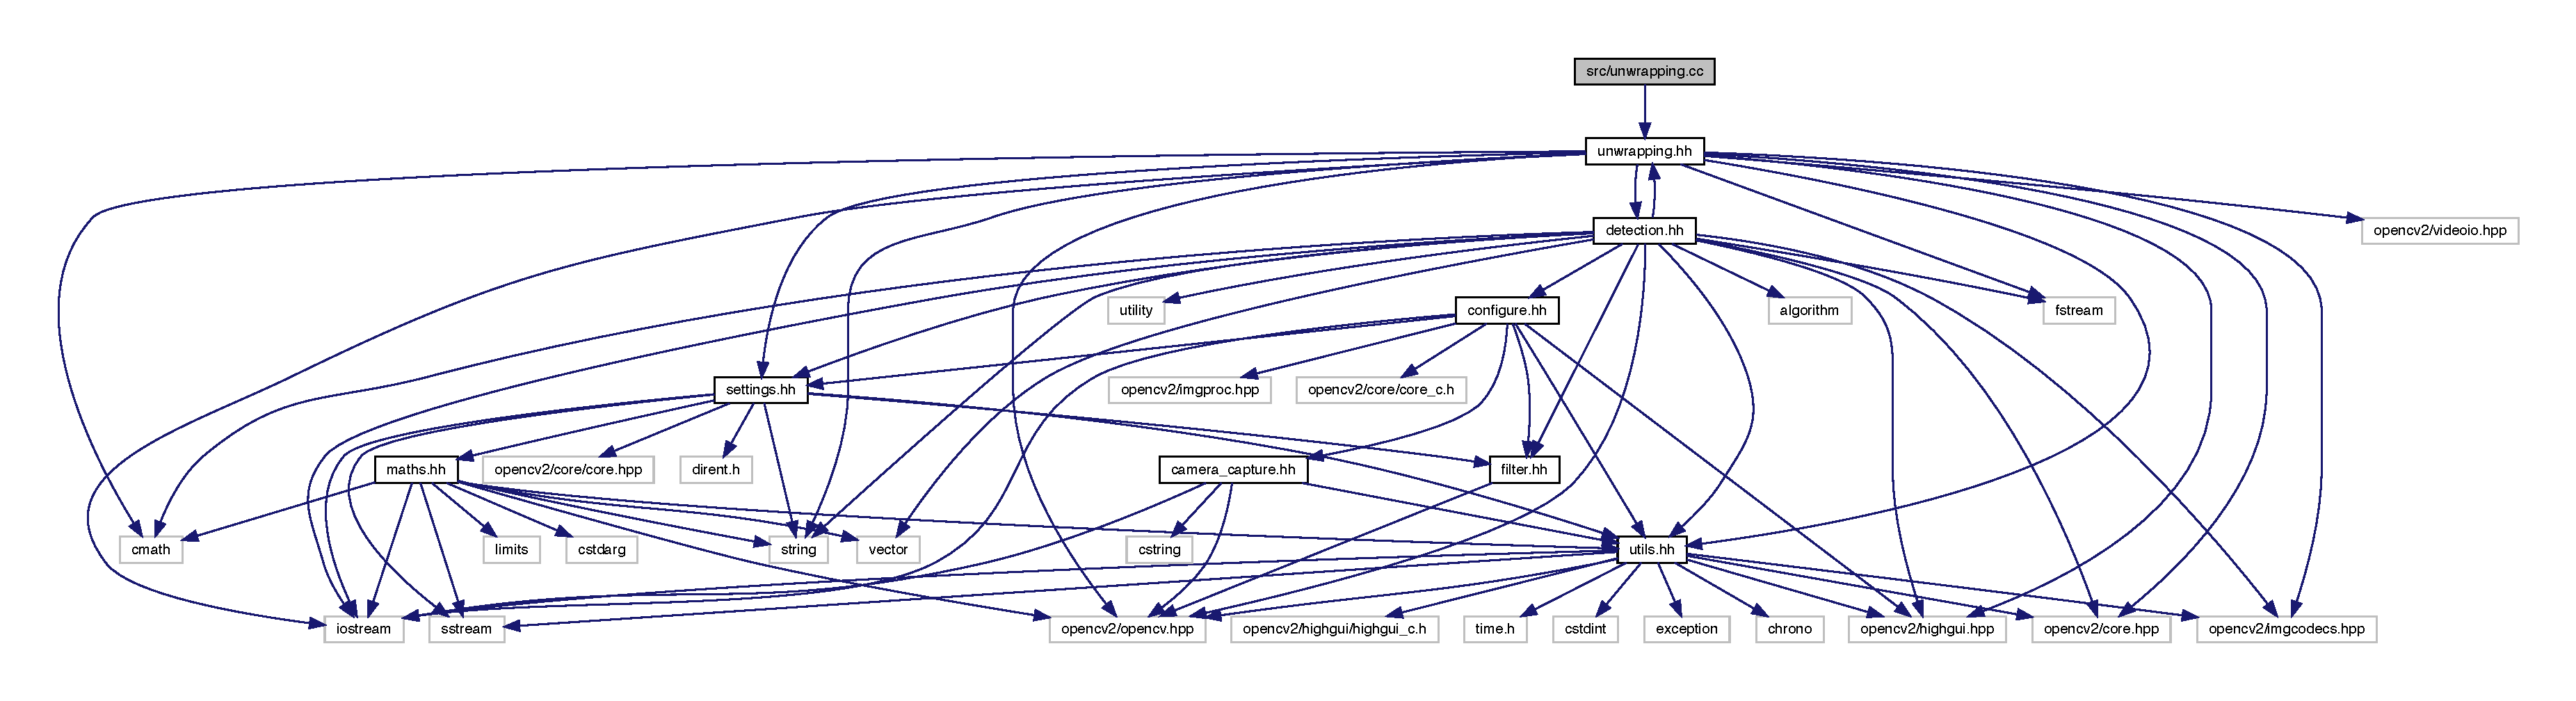
\includegraphics[width=350pt]{unwrapping_8cc__incl}
\end{center}
\end{figure}
\subsection*{Macros}
\begin{DoxyCompactItemize}
\item 
\#define \mbox{\hyperlink{unwrapping_8cc_a3c7ffff21a9a31fea3e9777b02d09291}{A\+R\+E\+A\+\_\+\+R\+A\+T\+IO}}~0.\+7
\item 
\#define \mbox{\hyperlink{unwrapping_8cc_ac2f75959ffa14bc8fd8d0491e890c122}{A\+R\+E\+A\+\_\+\+M\+IN}}~500
\end{DoxyCompactItemize}
\subsection*{Functions}
\begin{DoxyCompactItemize}
\item 
static float \mbox{\hyperlink{unwrapping_8cc_ac6bcc6db62057bda0b6195a11578fdfa}{distance}} (Point c1, Point c2)
\begin{DoxyCompactList}\small\item\em Compute the euclidean distance. \end{DoxyCompactList}\item 
\mbox{\hyperlink{draw_8hh_aa620a13339ac3a1177c86edc549fda9b}{int}} \mbox{\hyperlink{unwrapping_8cc_ae232c3264987d57a223a39226929da29}{unwrapping}} ()
\begin{DoxyCompactList}\small\item\em Take some images according to a xml and unwrap the black rectangle inside the image after appling undistortion trasformation. \end{DoxyCompactList}\item 
void \mbox{\hyperlink{unwrapping_8cc_ac30b4dbae9022e84e10ef97ba156c581}{find\+\_\+rect}} (vector$<$ Point $>$ \&\+\_\+rect, const \mbox{\hyperlink{draw_8hh_aa620a13339ac3a1177c86edc549fda9b}{int}} \&width, const \mbox{\hyperlink{draw_8hh_aa620a13339ac3a1177c86edc549fda9b}{int}} \&height)
\begin{DoxyCompactList}\small\item\em Since the border of the arena might not always be clean but might have some imperfection, this functions computes the four vertixes taking all the points and computing the four that are the clostest to the corner of the image. \end{DoxyCompactList}\item 
void \mbox{\hyperlink{unwrapping_8cc_a3cf7df08897ed4d1a7ddcf055b18cca8}{load\+Coefficients}} (const string filename, Mat \&camera\+\_\+matrix, Mat \&dist\+\_\+coeffs)
\begin{DoxyCompactList}\small\item\em Load coefficients from a file. \end{DoxyCompactList}\end{DoxyCompactItemize}


\subsection{Macro Definition Documentation}
\mbox{\Hypertarget{unwrapping_8cc_ac2f75959ffa14bc8fd8d0491e890c122}\label{unwrapping_8cc_ac2f75959ffa14bc8fd8d0491e890c122}} 
\index{unwrapping.cc@{unwrapping.cc}!AREA\_MIN@{AREA\_MIN}}
\index{AREA\_MIN@{AREA\_MIN}!unwrapping.cc@{unwrapping.cc}}
\subsubsection{\texorpdfstring{AREA\_MIN}{AREA\_MIN}}
{\footnotesize\ttfamily \#define A\+R\+E\+A\+\_\+\+M\+IN~500}

\mbox{\Hypertarget{unwrapping_8cc_a3c7ffff21a9a31fea3e9777b02d09291}\label{unwrapping_8cc_a3c7ffff21a9a31fea3e9777b02d09291}} 
\index{unwrapping.cc@{unwrapping.cc}!AREA\_RATIO@{AREA\_RATIO}}
\index{AREA\_RATIO@{AREA\_RATIO}!unwrapping.cc@{unwrapping.cc}}
\subsubsection{\texorpdfstring{AREA\_RATIO}{AREA\_RATIO}}
{\footnotesize\ttfamily \#define A\+R\+E\+A\+\_\+\+R\+A\+T\+IO~0.\+7}



\subsection{Function Documentation}
\mbox{\Hypertarget{unwrapping_8cc_ac6bcc6db62057bda0b6195a11578fdfa}\label{unwrapping_8cc_ac6bcc6db62057bda0b6195a11578fdfa}} 
\index{unwrapping.cc@{unwrapping.cc}!distance@{distance}}
\index{distance@{distance}!unwrapping.cc@{unwrapping.cc}}
\subsubsection{\texorpdfstring{distance()}{distance()}}
{\footnotesize\ttfamily static float distance (\begin{DoxyParamCaption}\item[{Point}]{c1,  }\item[{Point}]{c2 }\end{DoxyParamCaption})\hspace{0.3cm}{\ttfamily [static]}}



Compute the euclidean distance. 


\begin{DoxyParams}[1]{Parameters}
\mbox{\texttt{ in,out}}  & {\em c1} & The first point. \\
\hline
\mbox{\texttt{ in,out}}  & {\em c2} & The second point.\\
\hline
\end{DoxyParams}
\begin{DoxyReturn}{Returns}
The euclidean distance. 
\end{DoxyReturn}
\mbox{\Hypertarget{unwrapping_8cc_ac30b4dbae9022e84e10ef97ba156c581}\label{unwrapping_8cc_ac30b4dbae9022e84e10ef97ba156c581}} 
\index{unwrapping.cc@{unwrapping.cc}!find\_rect@{find\_rect}}
\index{find\_rect@{find\_rect}!unwrapping.cc@{unwrapping.cc}}
\subsubsection{\texorpdfstring{find\_rect()}{find\_rect()}}
{\footnotesize\ttfamily void find\+\_\+rect (\begin{DoxyParamCaption}\item[{vector$<$ Point $>$ \&}]{\+\_\+rect,  }\item[{const \mbox{\hyperlink{draw_8hh_aa620a13339ac3a1177c86edc549fda9b}{int}} \&}]{width,  }\item[{const \mbox{\hyperlink{draw_8hh_aa620a13339ac3a1177c86edc549fda9b}{int}} \&}]{height }\end{DoxyParamCaption})}



Since the border of the arena might not always be clean but might have some imperfection, this functions computes the four vertixes taking all the points and computing the four that are the clostest to the corner of the image. 


\begin{DoxyParams}[1]{Parameters}
\mbox{\texttt{ in}}  & {\em \+\_\+rect} & The vector of cv\+::\+Point to work on. \\
\hline
\mbox{\texttt{ in}}  & {\em width} & The width of the image. \\
\hline
\mbox{\texttt{ in}}  & {\em height} & The height of the image. \\
\hline
\end{DoxyParams}
\mbox{\Hypertarget{unwrapping_8cc_a3cf7df08897ed4d1a7ddcf055b18cca8}\label{unwrapping_8cc_a3cf7df08897ed4d1a7ddcf055b18cca8}} 
\index{unwrapping.cc@{unwrapping.cc}!loadCoefficients@{loadCoefficients}}
\index{loadCoefficients@{loadCoefficients}!unwrapping.cc@{unwrapping.cc}}
\subsubsection{\texorpdfstring{loadCoefficients()}{loadCoefficients()}}
{\footnotesize\ttfamily void load\+Coefficients (\begin{DoxyParamCaption}\item[{const string}]{filename,  }\item[{Mat \&}]{camera\+\_\+matrix,  }\item[{Mat \&}]{dist\+\_\+coeffs }\end{DoxyParamCaption})}



Load coefficients from a file. 

Load two matrix \textquotesingle{}camera\+\_\+matrix\textquotesingle{} and \textquotesingle{}distortion\+\_\+coefficients\textquotesingle{} from the xml file passed. 
\begin{DoxyParams}[1]{Parameters}
\mbox{\texttt{ in}}  & {\em filename} & The string that identify the location of the xml file. \\
\hline
\mbox{\texttt{ out}}  & {\em camera\+\_\+matrix} & Where the \textquotesingle{}camera\+\_\+matrix\textquotesingle{} matrix is saved. \\
\hline
\mbox{\texttt{ out}}  & {\em dist\+\_\+coeffs} & Where the \textquotesingle{}distortion\+\_\+coefficients\textquotesingle{} matrix is saved. \\
\hline
\end{DoxyParams}
\mbox{\Hypertarget{unwrapping_8cc_ae232c3264987d57a223a39226929da29}\label{unwrapping_8cc_ae232c3264987d57a223a39226929da29}} 
\index{unwrapping.cc@{unwrapping.cc}!unwrapping@{unwrapping}}
\index{unwrapping@{unwrapping}!unwrapping.cc@{unwrapping.cc}}
\subsubsection{\texorpdfstring{unwrapping()}{unwrapping()}}
{\footnotesize\ttfamily \mbox{\hyperlink{draw_8hh_aa620a13339ac3a1177c86edc549fda9b}{int}} unwrapping (\begin{DoxyParamCaption}{ }\end{DoxyParamCaption})}



Take some images according to a xml and unwrap the black rectangle inside the image after appling undistortion trasformation. 

Load from the xml file \textquotesingle{}data/settings.\+xml\textquotesingle{} the name of some images, load the images from the file,~\newline
apply the calibration (undistortion trasformation) thanks to the matrices load with the \textquotesingle{}load\+Coefficients\textquotesingle{} function.~\newline
Then, with the use of a filter for the black the region of interest (a rectangle) is identified and all the perspective is rotated for reach a top view of the rectangle.~\newline
Finally, the images are saved on some files.

\begin{DoxyReturn}{Returns}
A 0 is return if the function reach the end. 
\end{DoxyReturn}

\hypertarget{unwrapping_8hh}{}\section{src/include/unwrapping.hh File Reference}
\label{unwrapping_8hh}\index{src/include/unwrapping.hh@{src/include/unwrapping.hh}}
{\ttfamily \#include $<$utils.\+hh$>$}\newline
{\ttfamily \#include $<$settings.\+hh$>$}\newline
{\ttfamily \#include $<$iostream$>$}\newline
{\ttfamily \#include $<$fstream$>$}\newline
{\ttfamily \#include $<$string$>$}\newline
{\ttfamily \#include $<$cmath$>$}\newline
{\ttfamily \#include $<$opencv2/videoio.\+hpp$>$}\newline
{\ttfamily \#include $<$opencv2/highgui.\+hpp$>$}\newline
{\ttfamily \#include $<$opencv2/core.\+hpp$>$}\newline
{\ttfamily \#include $<$opencv2/opencv.\+hpp$>$}\newline
{\ttfamily \#include $<$opencv2/imgcodecs.\+hpp$>$}\newline
Include dependency graph for unwrapping.\+hh\+:
\nopagebreak
\begin{figure}[H]
\begin{center}
\leavevmode
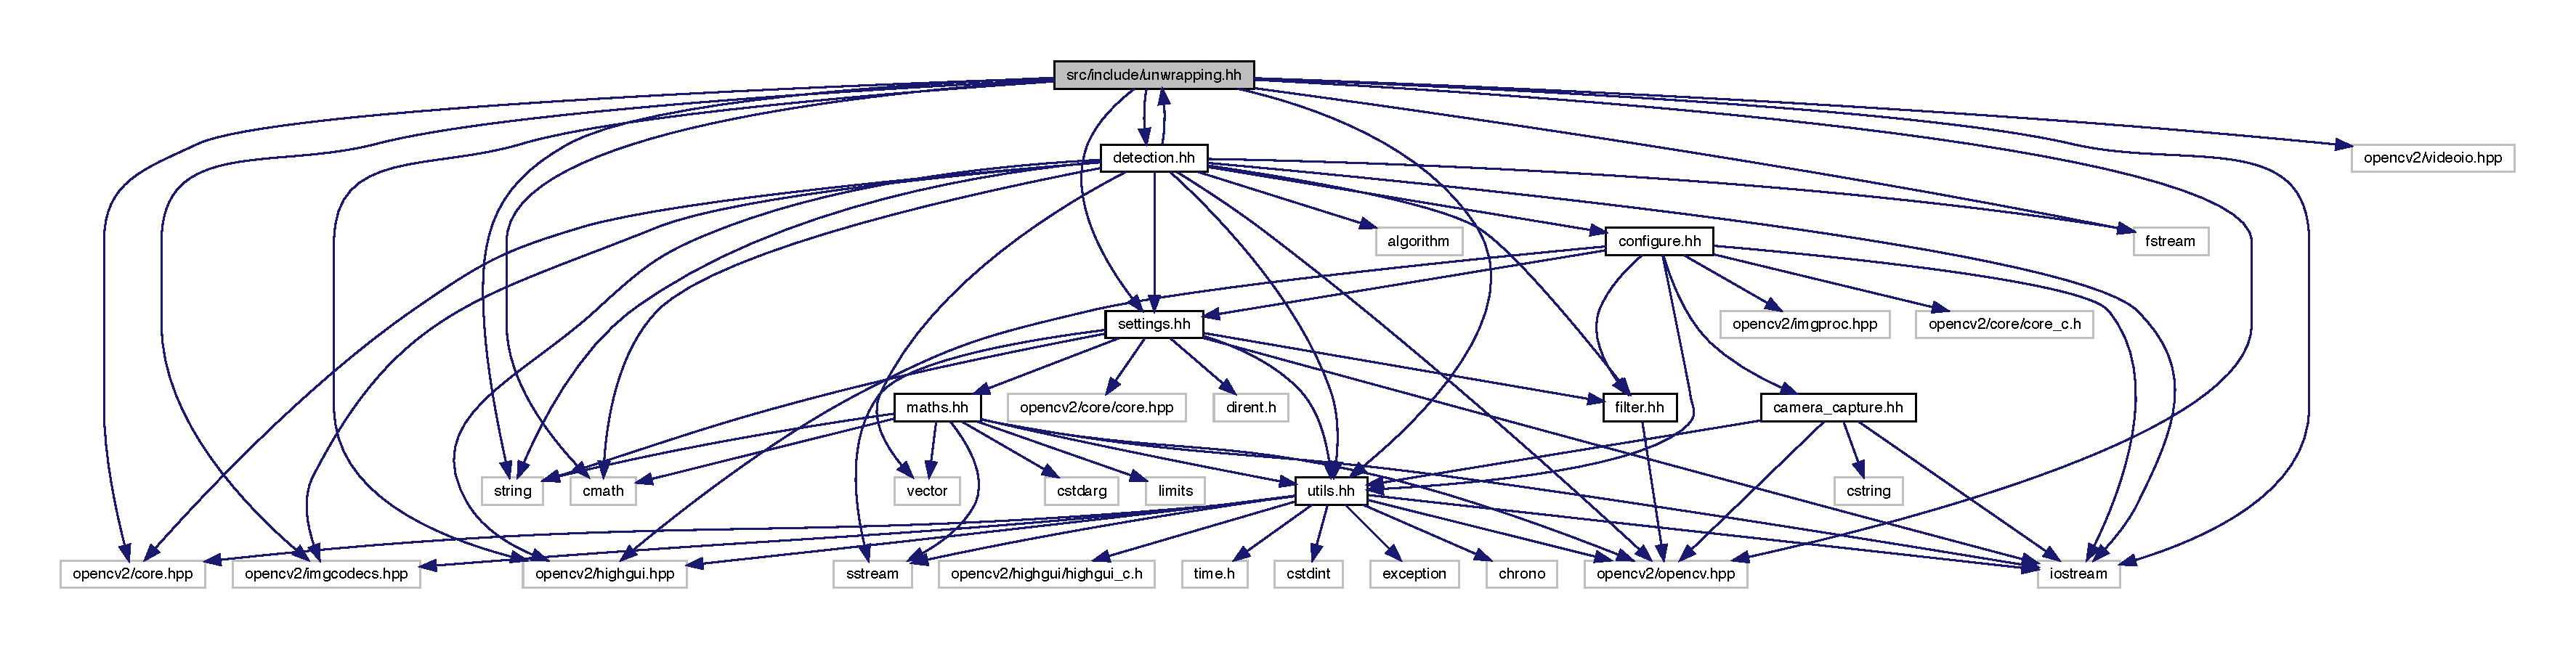
\includegraphics[width=350pt]{unwrapping_8hh__incl}
\end{center}
\end{figure}
This graph shows which files directly or indirectly include this file\+:
\nopagebreak
\begin{figure}[H]
\begin{center}
\leavevmode
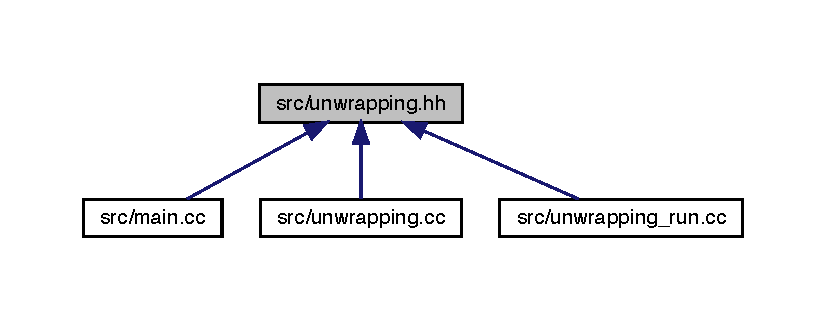
\includegraphics[width=350pt]{unwrapping_8hh__dep__incl}
\end{center}
\end{figure}
\subsection*{Functions}
\begin{DoxyCompactItemize}
\item 
\mbox{\hyperlink{draw_8hh_aa620a13339ac3a1177c86edc549fda9b}{int}} \mbox{\hyperlink{unwrapping_8hh_ae232c3264987d57a223a39226929da29}{unwrapping}} ()
\begin{DoxyCompactList}\small\item\em Take some images according to a xml and unwrap the black rectangle inside the image after appling undistortion trasformation. \end{DoxyCompactList}\item 
void \mbox{\hyperlink{unwrapping_8hh_a3cf7df08897ed4d1a7ddcf055b18cca8}{load\+Coefficients}} (const string filename, Mat \&camera\+\_\+matrix, Mat \&dist\+\_\+coeffs)
\begin{DoxyCompactList}\small\item\em Load coefficients from a file. \end{DoxyCompactList}\end{DoxyCompactItemize}


\subsection{Function Documentation}
\mbox{\Hypertarget{unwrapping_8hh_a3cf7df08897ed4d1a7ddcf055b18cca8}\label{unwrapping_8hh_a3cf7df08897ed4d1a7ddcf055b18cca8}} 
\index{unwrapping.hh@{unwrapping.hh}!loadCoefficients@{loadCoefficients}}
\index{loadCoefficients@{loadCoefficients}!unwrapping.hh@{unwrapping.hh}}
\subsubsection{\texorpdfstring{loadCoefficients()}{loadCoefficients()}}
{\footnotesize\ttfamily void load\+Coefficients (\begin{DoxyParamCaption}\item[{const string}]{filename,  }\item[{Mat \&}]{camera\+\_\+matrix,  }\item[{Mat \&}]{dist\+\_\+coeffs }\end{DoxyParamCaption})}



Load coefficients from a file. 

Load two matrix \textquotesingle{}camera\+\_\+matrix\textquotesingle{} and \textquotesingle{}distortion\+\_\+coefficients\textquotesingle{} from the xml file passed. 
\begin{DoxyParams}[1]{Parameters}
\mbox{\texttt{ in}}  & {\em filename} & The string that identify the location of the xml file. \\
\hline
\mbox{\texttt{ out}}  & {\em camera\+\_\+matrix} & Where the \textquotesingle{}camera\+\_\+matrix\textquotesingle{} matrix is saved. \\
\hline
\mbox{\texttt{ out}}  & {\em dist\+\_\+coeffs} & Where the \textquotesingle{}distortion\+\_\+coefficients\textquotesingle{} matrix is saved. \\
\hline
\end{DoxyParams}
\mbox{\Hypertarget{unwrapping_8hh_ae232c3264987d57a223a39226929da29}\label{unwrapping_8hh_ae232c3264987d57a223a39226929da29}} 
\index{unwrapping.hh@{unwrapping.hh}!unwrapping@{unwrapping}}
\index{unwrapping@{unwrapping}!unwrapping.hh@{unwrapping.hh}}
\subsubsection{\texorpdfstring{unwrapping()}{unwrapping()}}
{\footnotesize\ttfamily \mbox{\hyperlink{draw_8hh_aa620a13339ac3a1177c86edc549fda9b}{int}} unwrapping (\begin{DoxyParamCaption}{ }\end{DoxyParamCaption})}



Take some images according to a xml and unwrap the black rectangle inside the image after appling undistortion trasformation. 

Load from the xml file \textquotesingle{}data/settings.\+xml\textquotesingle{} the name of some images, load the images from the file,~\newline
apply the calibration (undistortion trasformation) thanks to the matrices load with the \textquotesingle{}load\+Coefficients\textquotesingle{} function.~\newline
Then, with the use of a filter for the black the region of interest (a rectangle) is identified and all the perspective is rotated for reach a top view of the rectangle.~\newline
Finally, the images are saved on some files.

\begin{DoxyReturn}{Returns}
A 0 is return if the function reach the end. 
\end{DoxyReturn}
File\+Storage fs\+\_\+xml(xml\+\_\+settings, File\+Storage\+::\+R\+E\+A\+D);

File\+Node Bm = s-\/$>$black\+Mask; 
\hypertarget{unwrapping__run_8cc}{}\section{src/run/unwrapping\+\_\+run.cc File Reference}
\label{unwrapping__run_8cc}\index{src/run/unwrapping\_run.cc@{src/run/unwrapping\_run.cc}}
{\ttfamily \#include $<$unwrapping.\+hh$>$}\newline
Include dependency graph for unwrapping\+\_\+run.\+cc\+:
\nopagebreak
\begin{figure}[H]
\begin{center}
\leavevmode
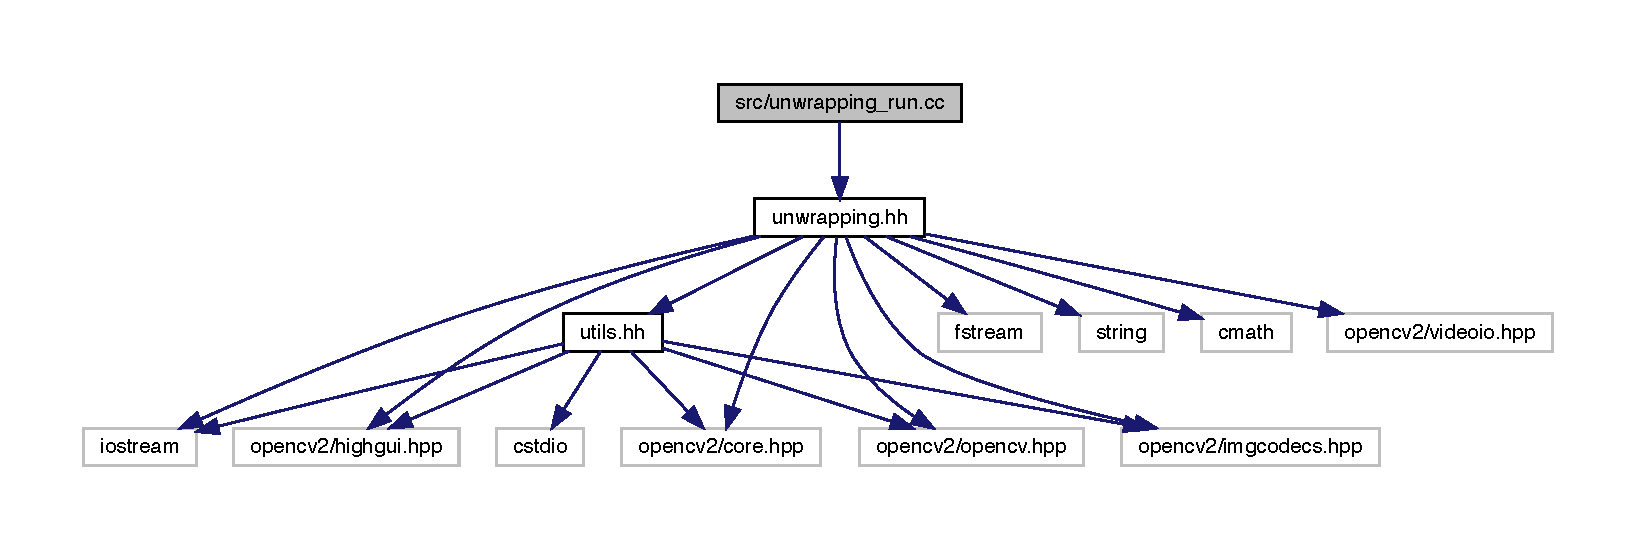
\includegraphics[width=350pt]{unwrapping__run_8cc__incl}
\end{center}
\end{figure}
\subsection*{Functions}
\begin{DoxyCompactItemize}
\item 
\mbox{\hyperlink{draw_8hh_aa620a13339ac3a1177c86edc549fda9b}{int}} \mbox{\hyperlink{unwrapping__run_8cc_ae66f6b31b5ad750f1fe042a706a4e3d4}{main}} ()
\end{DoxyCompactItemize}


\subsection{Function Documentation}
\mbox{\Hypertarget{unwrapping__run_8cc_ae66f6b31b5ad750f1fe042a706a4e3d4}\label{unwrapping__run_8cc_ae66f6b31b5ad750f1fe042a706a4e3d4}} 
\index{unwrapping\_run.cc@{unwrapping\_run.cc}!main@{main}}
\index{main@{main}!unwrapping\_run.cc@{unwrapping\_run.cc}}
\subsubsection{\texorpdfstring{main()}{main()}}
{\footnotesize\ttfamily \mbox{\hyperlink{draw_8hh_aa620a13339ac3a1177c86edc549fda9b}{int}} main (\begin{DoxyParamCaption}{ }\end{DoxyParamCaption})}


\hypertarget{utils_8cc}{}\section{src/utils.cc File Reference}
\label{utils_8cc}\index{src/utils.\+cc@{src/utils.\+cc}}
{\ttfamily \#include \char`\"{}utils.\+hh\char`\"{}}\newline
Include dependency graph for utils.\+cc\+:
\nopagebreak
\begin{figure}[H]
\begin{center}
\leavevmode
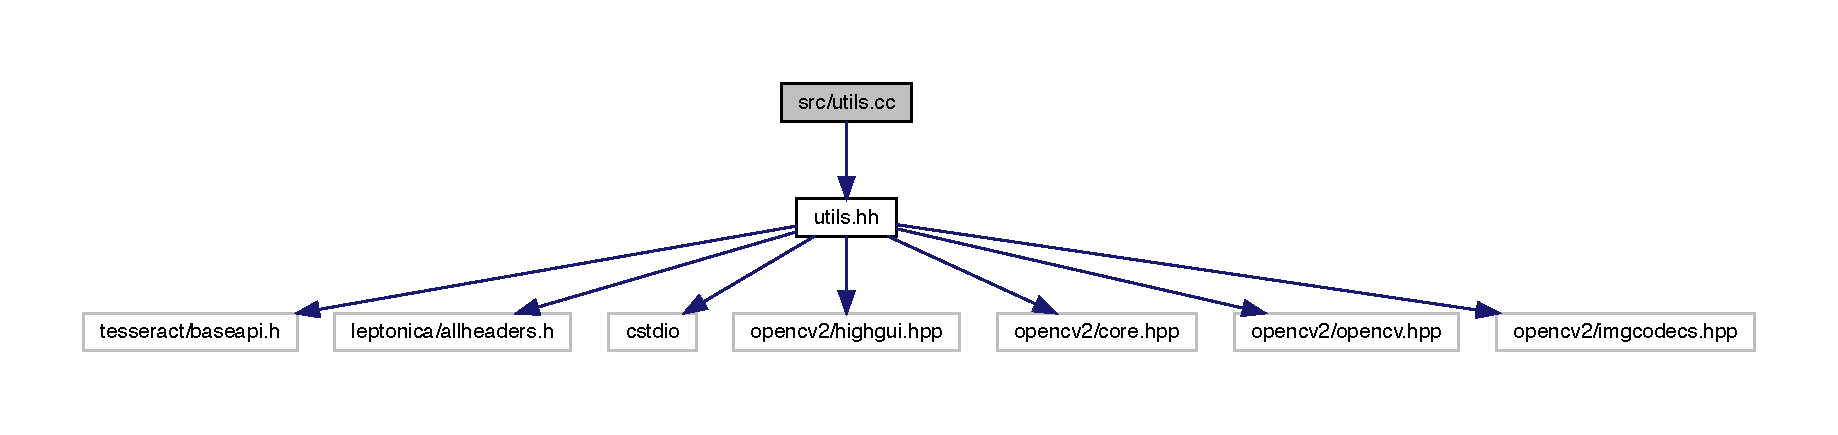
\includegraphics[width=350pt]{utils_8cc__incl}
\end{center}
\end{figure}
\subsection*{Functions}
\begin{DoxyCompactItemize}
\item 
void \mbox{\hyperlink{utils_8cc_a9a82362cf25a772ae278a98a68464c1f}{my\+\_\+imshow}} (const char $\ast$win\+\_\+name, Mat img, bool reset)
\end{DoxyCompactItemize}


\subsection{Function Documentation}
\mbox{\Hypertarget{utils_8cc_a9a82362cf25a772ae278a98a68464c1f}\label{utils_8cc_a9a82362cf25a772ae278a98a68464c1f}} 
\index{utils.\+cc@{utils.\+cc}!my\+\_\+imshow@{my\+\_\+imshow}}
\index{my\+\_\+imshow@{my\+\_\+imshow}!utils.\+cc@{utils.\+cc}}
\subsubsection{\texorpdfstring{my\+\_\+imshow()}{my\_imshow()}}
{\footnotesize\ttfamily void my\+\_\+imshow (\begin{DoxyParamCaption}\item[{const char $\ast$}]{win\+\_\+name,  }\item[{Mat}]{img,  }\item[{bool}]{reset }\end{DoxyParamCaption})}


\hypertarget{utils_8hh}{}\section{src/include/utils.hh File Reference}
\label{utils_8hh}\index{src/include/utils.hh@{src/include/utils.hh}}
{\ttfamily \#include $<$sstream$>$}\newline
{\ttfamily \#include $<$iostream$>$}\newline
{\ttfamily \#include $<$exception$>$}\newline
{\ttfamily \#include $<$chrono$>$}\newline
{\ttfamily \#include $<$opencv2/highgui.\+hpp$>$}\newline
{\ttfamily \#include $<$opencv2/highgui/highgui\+\_\+c.\+h$>$}\newline
{\ttfamily \#include $<$opencv2/core.\+hpp$>$}\newline
{\ttfamily \#include $<$opencv2/opencv.\+hpp$>$}\newline
{\ttfamily \#include $<$opencv2/imgcodecs.\+hpp$>$}\newline
{\ttfamily \#include $<$time.\+h$>$}\newline
{\ttfamily \#include $<$cstdint$>$}\newline
Include dependency graph for utils.\+hh\+:
\nopagebreak
\begin{figure}[H]
\begin{center}
\leavevmode
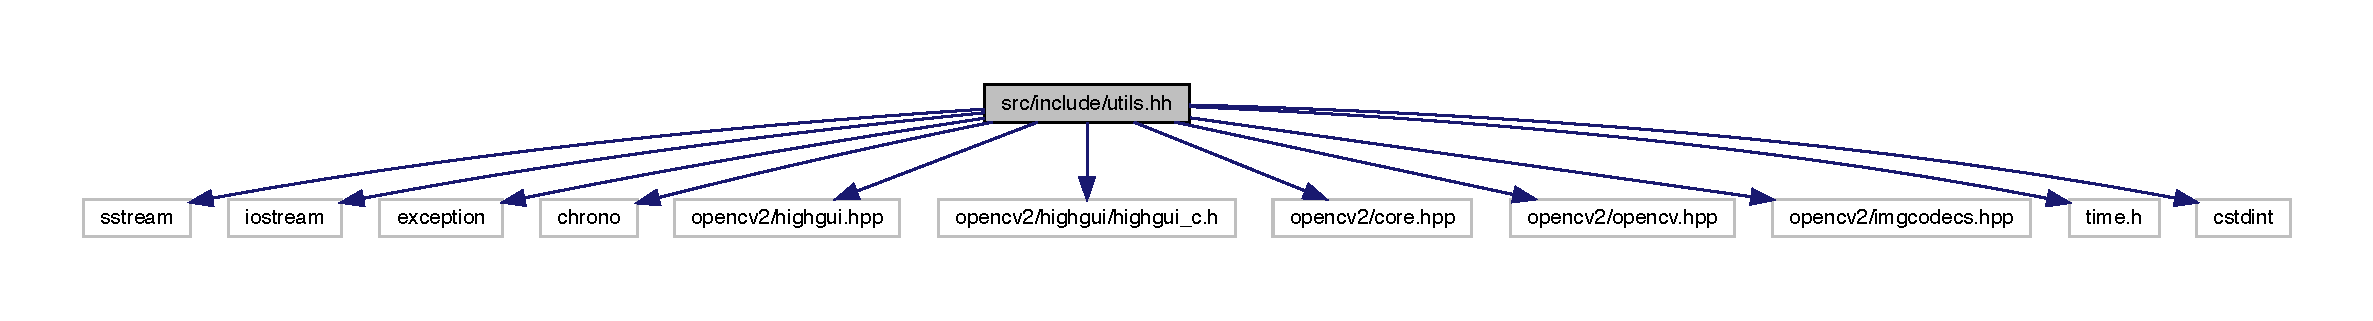
\includegraphics[width=350pt]{utils_8hh__incl}
\end{center}
\end{figure}
This graph shows which files directly or indirectly include this file\+:
\nopagebreak
\begin{figure}[H]
\begin{center}
\leavevmode
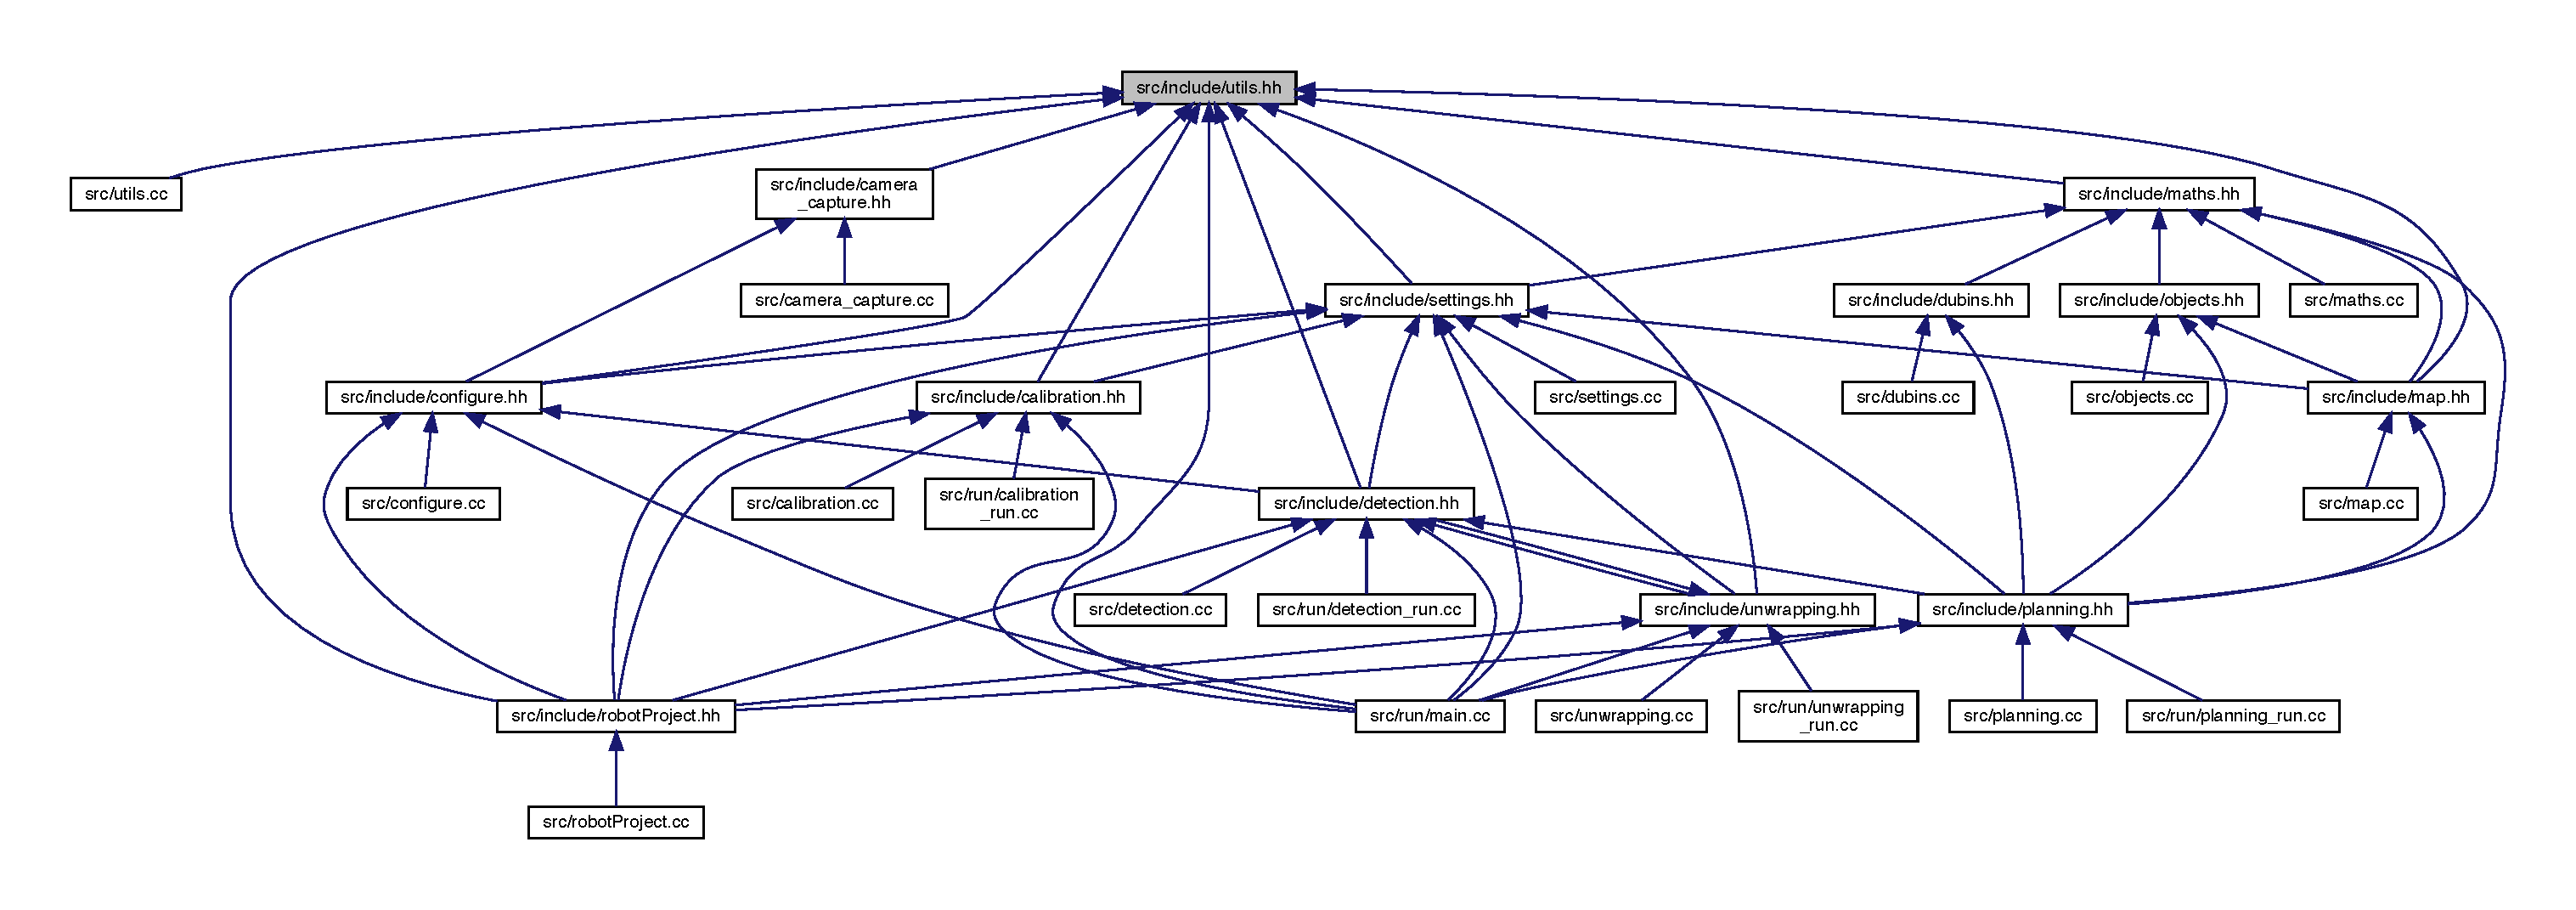
\includegraphics[width=350pt]{utils_8hh__dep__incl}
\end{center}
\end{figure}
\subsection*{Classes}
\begin{DoxyCompactItemize}
\item 
class \mbox{\hyperlink{class_my_exception}{My\+Exception$<$ T $>$}}
\end{DoxyCompactItemize}
\subsection*{Namespaces}
\begin{DoxyCompactItemize}
\item 
 \mbox{\hyperlink{namespace_c_h_r_o_n_o}{C\+H\+R\+O\+NO}}
\item 
 \mbox{\hyperlink{namespacetimeutils}{timeutils}}
\end{DoxyCompactItemize}
\subsection*{Macros}
\begin{DoxyCompactItemize}
\item 
\#define \mbox{\hyperlink{utils_8hh_a14111ac8f43949172b152e50dc720aba}{N\+A\+ME}}(x)~\#x
\begin{DoxyCompactList}\small\item\em Returns the name of the variable. \end{DoxyCompactList}\item 
\#define \mbox{\hyperlink{utils_8hh_a051dcff3fa35db18fbabb4fde1bd1167}{C\+O\+UT}}(x)
\begin{DoxyCompactList}\small\item\em Print a messag to stderr. \end{DoxyCompactList}\item 
\#define \mbox{\hyperlink{utils_8hh_a3ae64706314066fdc8b6c8029a915aa7}{I\+N\+FO}}(msg)
\begin{DoxyCompactList}\small\item\em Print the name of a variable and its content. Only if D\+E\+B\+UG is defined. \end{DoxyCompactList}\end{DoxyCompactItemize}
\subsection*{Typedefs}
\begin{DoxyCompactItemize}
\item 
typedef chrono\+::high\+\_\+resolution\+\_\+clock \mbox{\hyperlink{utils_8hh_af5fd44b7ee78ceeb4a0e869179f422f7}{Clock}}
\end{DoxyCompactItemize}
\subsection*{Enumerations}
\begin{DoxyCompactItemize}
\item 
enum \mbox{\hyperlink{namespace_c_h_r_o_n_o_a246e471488a6e6b17ddb86e3b817c7d9}{C\+H\+R\+O\+N\+O\+::\+T\+I\+M\+E\+\_\+\+T\+Y\+PE}} \{ \mbox{\hyperlink{namespace_c_h_r_o_n_o_a246e471488a6e6b17ddb86e3b817c7d9ac09415dca4fa7975506ab664d88b403a}{C\+H\+R\+O\+N\+O\+::\+S\+EC}}, 
\mbox{\hyperlink{namespace_c_h_r_o_n_o_a246e471488a6e6b17ddb86e3b817c7d9a2060724ab75592144c0b930e3394d845}{C\+H\+R\+O\+N\+O\+::\+M\+S\+EC}}, 
\mbox{\hyperlink{namespace_c_h_r_o_n_o_a246e471488a6e6b17ddb86e3b817c7d9aba8c3a9d281e3b934b74d5ff97a3a093}{C\+H\+R\+O\+N\+O\+::\+M\+U\+S\+EC}}, 
\mbox{\hyperlink{namespace_c_h_r_o_n_o_a246e471488a6e6b17ddb86e3b817c7d9a06ab3311d8f423104c3beae640896013}{C\+H\+R\+O\+N\+O\+::\+N\+S\+EC}}
 \}
\item 
enum \mbox{\hyperlink{utils_8hh_af26a5d951fd6ab4b44e6cd8425aa0383}{E\+X\+C\+E\+P\+T\+I\+O\+N\+\_\+\+T\+Y\+PE}} \{ \mbox{\hyperlink{utils_8hh_af26a5d951fd6ab4b44e6cd8425aa0383aa965658e6a84d5502df1c1987b0a8466}{G\+E\+N\+E\+R\+AL}}, 
\mbox{\hyperlink{utils_8hh_af26a5d951fd6ab4b44e6cd8425aa0383a3197625a1bb2264943f5a95f236d9973}{E\+X\+I\+S\+TS}}, 
\mbox{\hyperlink{utils_8hh_af26a5d951fd6ab4b44e6cd8425aa0383a4aa71180778b711338785695df5d7c52}{S\+I\+ZE}}
 \}
\end{DoxyCompactItemize}
\subsection*{Functions}
\begin{DoxyCompactItemize}
\item 
string \mbox{\hyperlink{namespace_c_h_r_o_n_o_ae2a3e41f8bf5f83ba84d3f4d2eed3836}{C\+H\+R\+O\+N\+O\+::get\+Type}} (T\+I\+M\+E\+\_\+\+T\+Y\+PE type, string ret=\char`\"{}\char`\"{})
\item 
double \mbox{\hyperlink{namespace_c_h_r_o_n_o_aebe2329c142a6f06b6fede41c3abf1b3}{C\+H\+R\+O\+N\+O\+::get\+Elapsed}} (Clock\+::time\+\_\+point start, Clock\+::time\+\_\+point stop, T\+I\+M\+E\+\_\+\+T\+Y\+PE type=M\+U\+S\+EC)
\item 
string \mbox{\hyperlink{namespace_c_h_r_o_n_o_ad8da7180c420d59f4c0077b60579c0ae}{C\+H\+R\+O\+N\+O\+::get\+Elapsed}} (Clock\+::time\+\_\+point start, Clock\+::time\+\_\+point stop, string ret, T\+I\+M\+E\+\_\+\+T\+Y\+PE type=M\+U\+S\+EC)
\item 
void \mbox{\hyperlink{utils_8hh_aabfea83501dfccfa4c420b8c19ceefd7}{my\+\_\+imshow}} (const char $\ast$win\+\_\+name, Mat img, bool reset=false)
\begin{DoxyCompactList}\small\item\em Function to show images in an order grill. \end{DoxyCompactList}\item 
void \mbox{\hyperlink{utils_8hh_af046ae860c3e4985ab0968caffb4c772}{mywaitkey}} (const char c=\textquotesingle{}q\textquotesingle{})
\begin{DoxyCompactList}\small\item\em Function to use after \mbox{\hyperlink{utils_8hh_aabfea83501dfccfa4c420b8c19ceefd7}{my\+\_\+imshow()}} for keeping the image opened until a key is pressed. \end{DoxyCompactList}\item 
void \mbox{\hyperlink{utils_8hh_a31ae190fba03c3a422a13a4271e0e424}{mywaitkey}} (string window\+Name)
\begin{DoxyCompactList}\small\item\em Function to use after \mbox{\hyperlink{utils_8hh_aabfea83501dfccfa4c420b8c19ceefd7}{my\+\_\+imshow()}} for keeping the image opened until a key is pressed. When a key is pressed a specific window is closed. \end{DoxyCompactList}\item 
int64\+\_\+t \mbox{\hyperlink{namespacetimeutils_a3d9d509a7028cffae8aef9c70f6c2c52}{timeutils\+::timespec\+Diff}} (struct timespec $\ast$time\+A\+\_\+p, struct timespec $\ast$time\+B\+\_\+p)
\item 
double \mbox{\hyperlink{namespacetimeutils_aa732b7f41462ff727daef77bd5030b9c}{timeutils\+::get\+TimeS}} ()
\end{DoxyCompactItemize}


\subsection{Macro Definition Documentation}
\mbox{\Hypertarget{utils_8hh_a051dcff3fa35db18fbabb4fde1bd1167}\label{utils_8hh_a051dcff3fa35db18fbabb4fde1bd1167}} 
\index{utils.hh@{utils.hh}!COUT@{COUT}}
\index{COUT@{COUT}!utils.hh@{utils.hh}}
\subsubsection{\texorpdfstring{COUT}{COUT}}
{\footnotesize\ttfamily \#define C\+O\+UT(\begin{DoxyParamCaption}\item[{}]{x }\end{DoxyParamCaption})}



Print a messag to stderr. 

\mbox{\Hypertarget{utils_8hh_a3ae64706314066fdc8b6c8029a915aa7}\label{utils_8hh_a3ae64706314066fdc8b6c8029a915aa7}} 
\index{utils.hh@{utils.hh}!INFO@{INFO}}
\index{INFO@{INFO}!utils.hh@{utils.hh}}
\subsubsection{\texorpdfstring{INFO}{INFO}}
{\footnotesize\ttfamily \#define I\+N\+FO(\begin{DoxyParamCaption}\item[{}]{msg }\end{DoxyParamCaption})}



Print the name of a variable and its content. Only if D\+E\+B\+UG is defined. 

\mbox{\Hypertarget{utils_8hh_a14111ac8f43949172b152e50dc720aba}\label{utils_8hh_a14111ac8f43949172b152e50dc720aba}} 
\index{utils.hh@{utils.hh}!NAME@{NAME}}
\index{NAME@{NAME}!utils.hh@{utils.hh}}
\subsubsection{\texorpdfstring{NAME}{NAME}}
{\footnotesize\ttfamily \#define N\+A\+ME(\begin{DoxyParamCaption}\item[{}]{x }\end{DoxyParamCaption})~\#x}



Returns the name of the variable. 



\subsection{Typedef Documentation}
\mbox{\Hypertarget{utils_8hh_af5fd44b7ee78ceeb4a0e869179f422f7}\label{utils_8hh_af5fd44b7ee78ceeb4a0e869179f422f7}} 
\index{utils.hh@{utils.hh}!Clock@{Clock}}
\index{Clock@{Clock}!utils.hh@{utils.hh}}
\subsubsection{\texorpdfstring{Clock}{Clock}}
{\footnotesize\ttfamily typedef chrono\+::high\+\_\+resolution\+\_\+clock \mbox{\hyperlink{utils_8hh_af5fd44b7ee78ceeb4a0e869179f422f7}{Clock}}}



\subsection{Enumeration Type Documentation}
\mbox{\Hypertarget{utils_8hh_af26a5d951fd6ab4b44e6cd8425aa0383}\label{utils_8hh_af26a5d951fd6ab4b44e6cd8425aa0383}} 
\index{utils.hh@{utils.hh}!EXCEPTION\_TYPE@{EXCEPTION\_TYPE}}
\index{EXCEPTION\_TYPE@{EXCEPTION\_TYPE}!utils.hh@{utils.hh}}
\subsubsection{\texorpdfstring{EXCEPTION\_TYPE}{EXCEPTION\_TYPE}}
{\footnotesize\ttfamily enum \mbox{\hyperlink{utils_8hh_af26a5d951fd6ab4b44e6cd8425aa0383}{E\+X\+C\+E\+P\+T\+I\+O\+N\+\_\+\+T\+Y\+PE}}}

\begin{DoxyEnumFields}{Enumerator}
\raisebox{\heightof{T}}[0pt][0pt]{\index{GENERAL@{GENERAL}!utils.hh@{utils.hh}}\index{utils.hh@{utils.hh}!GENERAL@{GENERAL}}}\mbox{\Hypertarget{utils_8hh_af26a5d951fd6ab4b44e6cd8425aa0383aa965658e6a84d5502df1c1987b0a8466}\label{utils_8hh_af26a5d951fd6ab4b44e6cd8425aa0383aa965658e6a84d5502df1c1987b0a8466}} 
G\+E\+N\+E\+R\+AL&\\
\hline

\raisebox{\heightof{T}}[0pt][0pt]{\index{EXISTS@{EXISTS}!utils.hh@{utils.hh}}\index{utils.hh@{utils.hh}!EXISTS@{EXISTS}}}\mbox{\Hypertarget{utils_8hh_af26a5d951fd6ab4b44e6cd8425aa0383a3197625a1bb2264943f5a95f236d9973}\label{utils_8hh_af26a5d951fd6ab4b44e6cd8425aa0383a3197625a1bb2264943f5a95f236d9973}} 
E\+X\+I\+S\+TS&\\
\hline

\raisebox{\heightof{T}}[0pt][0pt]{\index{SIZE@{SIZE}!utils.hh@{utils.hh}}\index{utils.hh@{utils.hh}!SIZE@{SIZE}}}\mbox{\Hypertarget{utils_8hh_af26a5d951fd6ab4b44e6cd8425aa0383a4aa71180778b711338785695df5d7c52}\label{utils_8hh_af26a5d951fd6ab4b44e6cd8425aa0383a4aa71180778b711338785695df5d7c52}} 
S\+I\+ZE&\\
\hline

\end{DoxyEnumFields}


\subsection{Function Documentation}
\mbox{\Hypertarget{utils_8hh_aabfea83501dfccfa4c420b8c19ceefd7}\label{utils_8hh_aabfea83501dfccfa4c420b8c19ceefd7}} 
\index{utils.hh@{utils.hh}!my\_imshow@{my\_imshow}}
\index{my\_imshow@{my\_imshow}!utils.hh@{utils.hh}}
\subsubsection{\texorpdfstring{my\_imshow()}{my\_imshow()}}
{\footnotesize\ttfamily void my\+\_\+imshow (\begin{DoxyParamCaption}\item[{const char $\ast$}]{win\+\_\+name,  }\item[{Mat}]{img,  }\item[{bool}]{reset = {\ttfamily false} }\end{DoxyParamCaption})}



Function to show images in an order grill. 


\begin{DoxyParams}{Parameters}
{\em win\+\_\+name} & The name of the window to use. \\
\hline
{\em img} & The Mat containing the image. \\
\hline
{\em reset} & If true the image is going to be placed in 0,0 i.\+e. the top left corner of the screen. \\
\hline
\end{DoxyParams}
\mbox{\Hypertarget{utils_8hh_af046ae860c3e4985ab0968caffb4c772}\label{utils_8hh_af046ae860c3e4985ab0968caffb4c772}} 
\index{utils.hh@{utils.hh}!mywaitkey@{mywaitkey}}
\index{mywaitkey@{mywaitkey}!utils.hh@{utils.hh}}
\subsubsection{\texorpdfstring{mywaitkey()}{mywaitkey()}\hspace{0.1cm}{\footnotesize\ttfamily [1/2]}}
{\footnotesize\ttfamily void mywaitkey (\begin{DoxyParamCaption}\item[{const char}]{c }\end{DoxyParamCaption})}



Function to use after \mbox{\hyperlink{utils_8hh_aabfea83501dfccfa4c420b8c19ceefd7}{my\+\_\+imshow()}} for keeping the image opened until a key is pressed. 

\mbox{\Hypertarget{utils_8hh_a31ae190fba03c3a422a13a4271e0e424}\label{utils_8hh_a31ae190fba03c3a422a13a4271e0e424}} 
\index{utils.hh@{utils.hh}!mywaitkey@{mywaitkey}}
\index{mywaitkey@{mywaitkey}!utils.hh@{utils.hh}}
\subsubsection{\texorpdfstring{mywaitkey()}{mywaitkey()}\hspace{0.1cm}{\footnotesize\ttfamily [2/2]}}
{\footnotesize\ttfamily void mywaitkey (\begin{DoxyParamCaption}\item[{string}]{window\+Name }\end{DoxyParamCaption})}



Function to use after \mbox{\hyperlink{utils_8hh_aabfea83501dfccfa4c420b8c19ceefd7}{my\+\_\+imshow()}} for keeping the image opened until a key is pressed. When a key is pressed a specific window is closed. 


\begin{DoxyParams}{Parameters}
{\em window\+Name} & The window to close after pressing a key. \\
\hline
\end{DoxyParams}

%--- End generated contents ---

% Index
\backmatter
\newpage
\phantomsection
\clearemptydoublepage
\addcontentsline{toc}{chapter}{Index}
\printindex

\end{document}
